% !TeX spellcheck = en_US
% !TeX encoding = UTF-8
\documentclass[aps, 11pt, a4paper]{article}
\usepackage{graphics, graphicx}
\usepackage{fancyvrb, enumerate}
\usepackage{amsmath, amssymb, amscd, amsfonts}
\usepackage{geometry}
\usepackage{multirow}
\usepackage{url}
\usepackage{tikz}
\usepackage{listings, listing}
\usepackage{color}
\usepackage{mathptmx}

\usetikzlibrary{shapes, arrows, calc, positioning}
\definecolor{codegreen}{rgb}{0, 0.6, 0}
\definecolor{codegray}{rgb}{0.5, 0.5, 0.5}
\definecolor{codepurple}{rgb}{0.58, 0, 0.82}
\definecolor{backcolour}{rgb}{0.95, 0.95, 0.92}
\lstdefinestyle{mystyle}
{
    backgroundcolor=\color{backcolour},   
    commentstyle=\color{codegreen},
    keywordstyle=\color{magenta},
    numberstyle=\tiny\color{codegray},
    stringstyle=\color{codepurple},
    basicstyle=\footnotesize,
    breakatwhitespace=false,         
    breaklines=true,                 
    captionpos=b,                    
    keepspaces=true,                 
    numbers=left,                    
    numbersep=5pt,                  
    showspaces=false,                
    showstringspaces=false,
    showtabs=false,                  
    tabsize=2,
    frame=single
}
\lstset{style=mystyle}
\tikzstyle{decision} = [diamond, draw, fill=blue!20, text width=4.5em, text badly centered, node distance=3cm, inner sep=0pt]
\tikzstyle{block} = [rectangle, draw, fill=blue!20, text width=5em, text centered, rounded corners, minimum height=2em]
\tikzstyle{line} = [draw, -latex']
\tikzstyle{cloud} = [draw, ellipse, fill=red!20, node distance=5em, minimum height=2em]
\tikzset
{
    -|-/.style=
    {
        to path=
        {
            (\tikztostart) -| ($(\tikztostart)!#1!(\tikztotarget)$) |- (\tikztotarget)
            \tikztonodes
        }
    },
    -|-/.default=0.5,
    |-|/.style=
    {
        to path=
        {
            (\tikztostart) |- ($(\tikztostart)!#1!(\tikztotarget)$) -| (\tikztotarget)
            \tikztonodes
        }
    },
    |-|/.default=0.5,
}
\geometry
{
    top = 20mm,
    bottom = 20mm,
    left = 20mm,
    right = 20mm
}

\title{Prediction for Periodontists by Oral Bacteria in Korean\\ \large 2020 1st Semester Interdisciplinary Project}
\author{20161206 JaewoongLee}
\date{\today}

\begin{document}
    \maketitle
    \begin{table}[h]
    	\centering
		\begin{tabular}{c|c}
			Student ID & 20161206 \\ \hline
			Name & Jaewoong Lee \\ \hline
			School & School of Electrical \& Computer Engineering \\ \hline
			1 Track & Computer Science \& Engineering \\ \hline
			2 Track & Bio-medical Engineering \\ \hline
			Advisor 1 & Prof. Sungahn Ko \\ \hline
			Advisor 2 & Prof. Semin Lee \\
		\end{tabular}
    \end{table}
    \newpage
    
    \tableofcontents
    \listoftables
    \listoffigures
    \newpage
    
    \section{Introduction}
    	\subsection{Periodontitis}
    		Periodontitis is an inflammatory disease of the periodontium which is characterized by a progressive destruction of the tissues supporting the tooth \cite{ref:perio2}. In histopathologically, periodontitis may result periodontal pocketing, location of junctional epithelium apical to the cemento-enamal junction, loss of collagen fibers subjacent to the pocket epithelium, numerous poly-morphonuclear leukocytes in epithelium and a dense inflammatory cell infiltrate with plasma cells, lymphocytes, and macrophages \cite{ref:perio1}. Periodontits is currently assumed to progress as periodic, relatively short episodes of rapid tissue destruction followed by some prolonged intervening periods of disease remission \cite{ref:perio2}. 
    		
    		\begin{figure}[htbp]
    			\centering
    			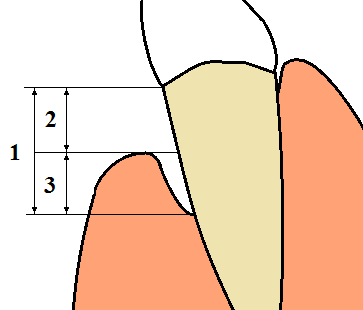
\includegraphics[width=0.3 \linewidth]{figures/recession.png}
    			\caption{Diagram of Gingival Recession \protect \cite{ref:depth1}}
    			\label{fig:depth}
    		\end{figure}
    	
    		Periodontitis is diagnosed by measuring clinical attachment loss (CAL). Note that the CAL is the length of the figure \ref{fig:depth}-1, which is sum of gingival recession (GR) in figure \ref{fig:depth}-2, and probing depth (PD) in figure \ref{fig:depth}-3.
    		
    		Periodontitis is generally believed to be a result of a host-parasite interaction in which bacteria are the determinants of periodontitis \cite{ref:cause1}. In etiology, the primary cause of periodontitis is presumed as a bacterial infection as the primary cause of periodontitis \cite{ref:perio1}. Thus, the treatment of periodontitis includes antibiotics and dental surgery.
    		
    		In this manner, some medicines have been introduced for treatment. However, the success in the prevention and treatment of periodontitis has been limited. Many \textit{in vitro} studies shows that Asian have the different bacteria from non-Asian, due to their groceries \cite{ref:asian1}. Thus, the developments of plaque and calculus in Asian differ, and may lead to distant reactions between Asian and non-Asian.
    		
    	\subsection{Machine Learning}
    		Machine learning is the study of algorithms which advance spontaneously through experience. Machine learning is conjugated where is infeasible with conventional algorithms such as computer vision.  Many papers show that machine learning brings out better result than human recognition. 
    	
    		If the feedback provides the correct answer for specific inputs, then learning problem is called supervised learning \cite{ref:ai1}. Classification is a kind of supervised learning for discrete values; regression is for continuous values.
    		
    	\subsection{Purpose of Research}
    		There are many studies which have tried to find bacteria as bio-markers \cite{ref:biomarker1, ref:biomarker2}. Most of these papers, though, researched in Western people \cite{ref:west1, ref:west2}. As I mentioned herein-above, oral bacteria population may differ between Western and non-Western. In this approach, therefore, prediction periodontitis from machine learning which based on oral bacteria population of Korean is required. 
    		
			I aimed to probe the performance of machine learning which predict the severity of periodontitis. Specifically, the purpose of this research is herein-after:
    		\begin{enumerate}
				\item Classify the stage of periodontitis by oral bacteria.
				\item Regress the CAL, the GR, or the PD by oral bacteria. 
    		\end{enumerate}
    
    \section{Materials}
    	\subsection{Clinical Examinations}
	    	This study included 784 samples from who visited the Department of Periodontics, Pusan National University Dental Hospital, between August 2016 and March 2019. The study protocol was approved by the Institutional Review Board of Pusan National University Dental Hospital (PNUDH-2016-019). All samples are provided written informed consent upon complete information regarding the objectives and procedures of this study.
	    	
	    	The diagnosis of samples was completed as \cite{ref:diagnosis1}. Also, the stage of periodontitis was categorized on the basis of the CAL as following:
	    	\begin{itemize}
	    		\item Healthy: $\leq$ 1mm
				\item Slight: 1-2 mm
				\item Moderate: 3-4 mm
				\item Severe: $\geq$ 5 mm
	    	\end{itemize}
	    
	    	Moreover, the following patients were excluded:
	    	\begin{itemize}
				\item who received periodontal treatment with past six months
				\item who were pregnant or breastfeeding
				\item who refused to approve the informed consent form
	    	\end{itemize}
	    
	    	The CAL was measured with a periodontal probe (PGF-W, Osung, Kwangmyung, Republic of Korea) during the clinical evaluation. All measurement were performed by two fully-experienced periodontitsts.
	    
	    \subsection{Analysis of Bacterial Copy}
	    	Collection of mouthwash sample and DAN extraction were performed as \cite{ref:DNA1}. Also, the nine pathogens were chosen as herein-after:
	    	\begin{enumerate}
				\item \textit{Porphyromonas gingivalis (Pg)}
				\item \textit{Tannerella forsysthia (Tf)}
				\item \textit{Treponema denticola (Td)}
				\item \textit{Prevotella intermedia (Pi)}
				\item \textit{Fusobacterium nucleatum (Fn)}
				\item \textit{Campylobacter rectus (Cr)}
				\item \textit{Aggregatibacter actinomycetemcomitans (Aa)}
				\item \textit{Peptostreptococcus anaerobius (Pa)}
				\item \textit{Eikenella corrodens (Ec)}
	    	\end{enumerate}
    	
    		Multiplex qPCR system was optimized for the nine pathogens after the building of standard curves for each pathogen. 
    
    \section{Methods}
    	The entire program is disclosed by GitHub in \url{https://github.com/Fumire/Periodontist_Fall2019}. 
    
    	\subsection{Python Packages}
    		Python programming language had been used to analyze data. Also, many Python modules had been adopted as hereinafter.
    		
    		\subsubsection{Pandas}
    		\textit{Pandas} is a Python library of rich data structures and tools for working with structured data sets common to statistics, finances, social sciences, and many other fields \cite{ref:pandas1}.
    		
    		\subsubsection{Scikit-learn: Machine Learning in Python}
    			\textit{Scikit-learn} is a Python module integrating a wide range of state-of-the-art machine learning algorithms for medium-scale supervised and unsupervised problems \cite{ref:sklearn1}.``
    			    			
    		\subsubsection{Seaborn}
		   		\textit{Seaborn} is a Python data visualization library based on \textit{matplotlib}. It provides a high-level interface for drawing attractive and informative statistics graphics \cite{ref:seaborn1}.
		
			\subsection{Classification}
				In classification, every combination of the nine pathogens, $2^9 = 512$ combinations, will be used. Also, in classification, some classes are merged into new class. For instance, healthy class and slight class could be merged, then the algorithm will be performed with four classes. As the pathogen combination, every combination of merging classes will be finished. 
				
				\subsubsection{Confusion Matrix and Its Derivations}
					A confusion matrix is a table which displays the performance of classification algorithm. Typically, the confusion matrix is like as table \ref{tb:confusion}.
					
					\begin{table}[htbp]
						\centering
						\caption{Abstract Form of Confusion Matrix}
						\label{tb:confusion}
						\begin{tabular}{cc|cc}
							\multicolumn{2}{c}{\multirow{2}{*}{}} & \multicolumn{2}{|c}{Actual Class} \\ \cline{3-4} 
							\multicolumn{2}{c|}{} & Positive & Negative \\ \hline
							\multicolumn{1}{c|}{\multirow{2}{*}{Predicted Class}} & Positive & True Positive & False Positive \\
							\multicolumn{1}{c|}{} & Negative & False Negative & True Negative
						\end{tabular}
					\end{table}
					
					Many derivations, such as sensitivity and specificity, come from the confusion matrix. The equation of derivations are followings:
					\begin{itemize}
						\item Sensitivity = $\frac{TP}{P}$
						\item Specificity = $\frac{TN}{N}$
						\item Precision = $\frac{TP}{TP + FP}$
						\item Negative predictive value = $\frac{TN}{TN + FN}$
						\item Miss rate = $\frac{FN}{P}$ = $\frac{FN}{FN + TP}$
						\item False positive rate = $\frac{FP}{N}$ = $\frac{FP}{FP + TN}$
						\item False discovery rate = $\frac{FP}{FP + TP}$
						\item False omission rate = $\frac{FN}{FN + TN}$
						\item Threat score = $\frac{TP}{TP + FN + FP}$
						\item Accuracy = $\frac{TP+TN}{P + N}$
						\item F1 score = $\frac{2TP}{2TP + FP + FN}$
					\end{itemize}
					
					Note that followed abbreviations are used:
					\begin{itemize}
						\item P: Positive
						\item N: Negative
						\item TP: True Positive
						\item TN: True Negative
						\item FP: False Positive
						\item FN: False Negative
					\end{itemize}
				
			\subsubsection{Classification Algorithm}
				For classification, the followed algorithms has been used:
				\begin{itemize}
					\item K-Neighbors
					\item Linear Support Vector Classification (SVC)
					\item Poly SVC
					\item RBF SVC
					\item Sigmoid SVC
					\item Decision Tree
					\item Random Forest
					\item Adam Neural Network (NN)
					\item lbfgs NN
					\item Ada-Boost
				\end{itemize}
				These are almost every algorithm which are supported by \textit{Scikit-learn}.
				
		\subsection{Regression}
			In regression, every combination of the nine pathogens, $2^9 = 512$ combinations, will be used. 
			\subsubsection{Coefficient of Determination}
				Coefficient of determination, also known as $R^2$ or R-square, is common to use as an index of the size of the relation \cite{ref:rsquare1}. 
				
			\subsubsection{Regression Algorithm}
				For regression, the followed algorithm has been used:
				\begin{itemize}
					\item Linear Regression
					\item Ridge
					\item Support Vector Regression (SVR)
					\item Nu SVR
					\item Linear SVR
					\item Elastic Network
					\item K-Neighbors
					\item Decision Tree
					\item lbfgs Multi-Layer Perceptron (MLP)
					\item sgd MLP
				\end{itemize}
				These are almost every algorithm which are supported by \textit{Scikit-learn}.
    
    \section{Results}
    	\subsection{5-class Classification}
    		Figure \ref{fig:5-confusion} displays the derivations of confusion matrix in 5-class classification. Note that the values in figure \ref{fig:5-confusion}, mean values from combinations which used same number of features will be shown. 
    		
    		\begin{figure}[htbp]
				\centering
				$\begin{array}{ccc}
					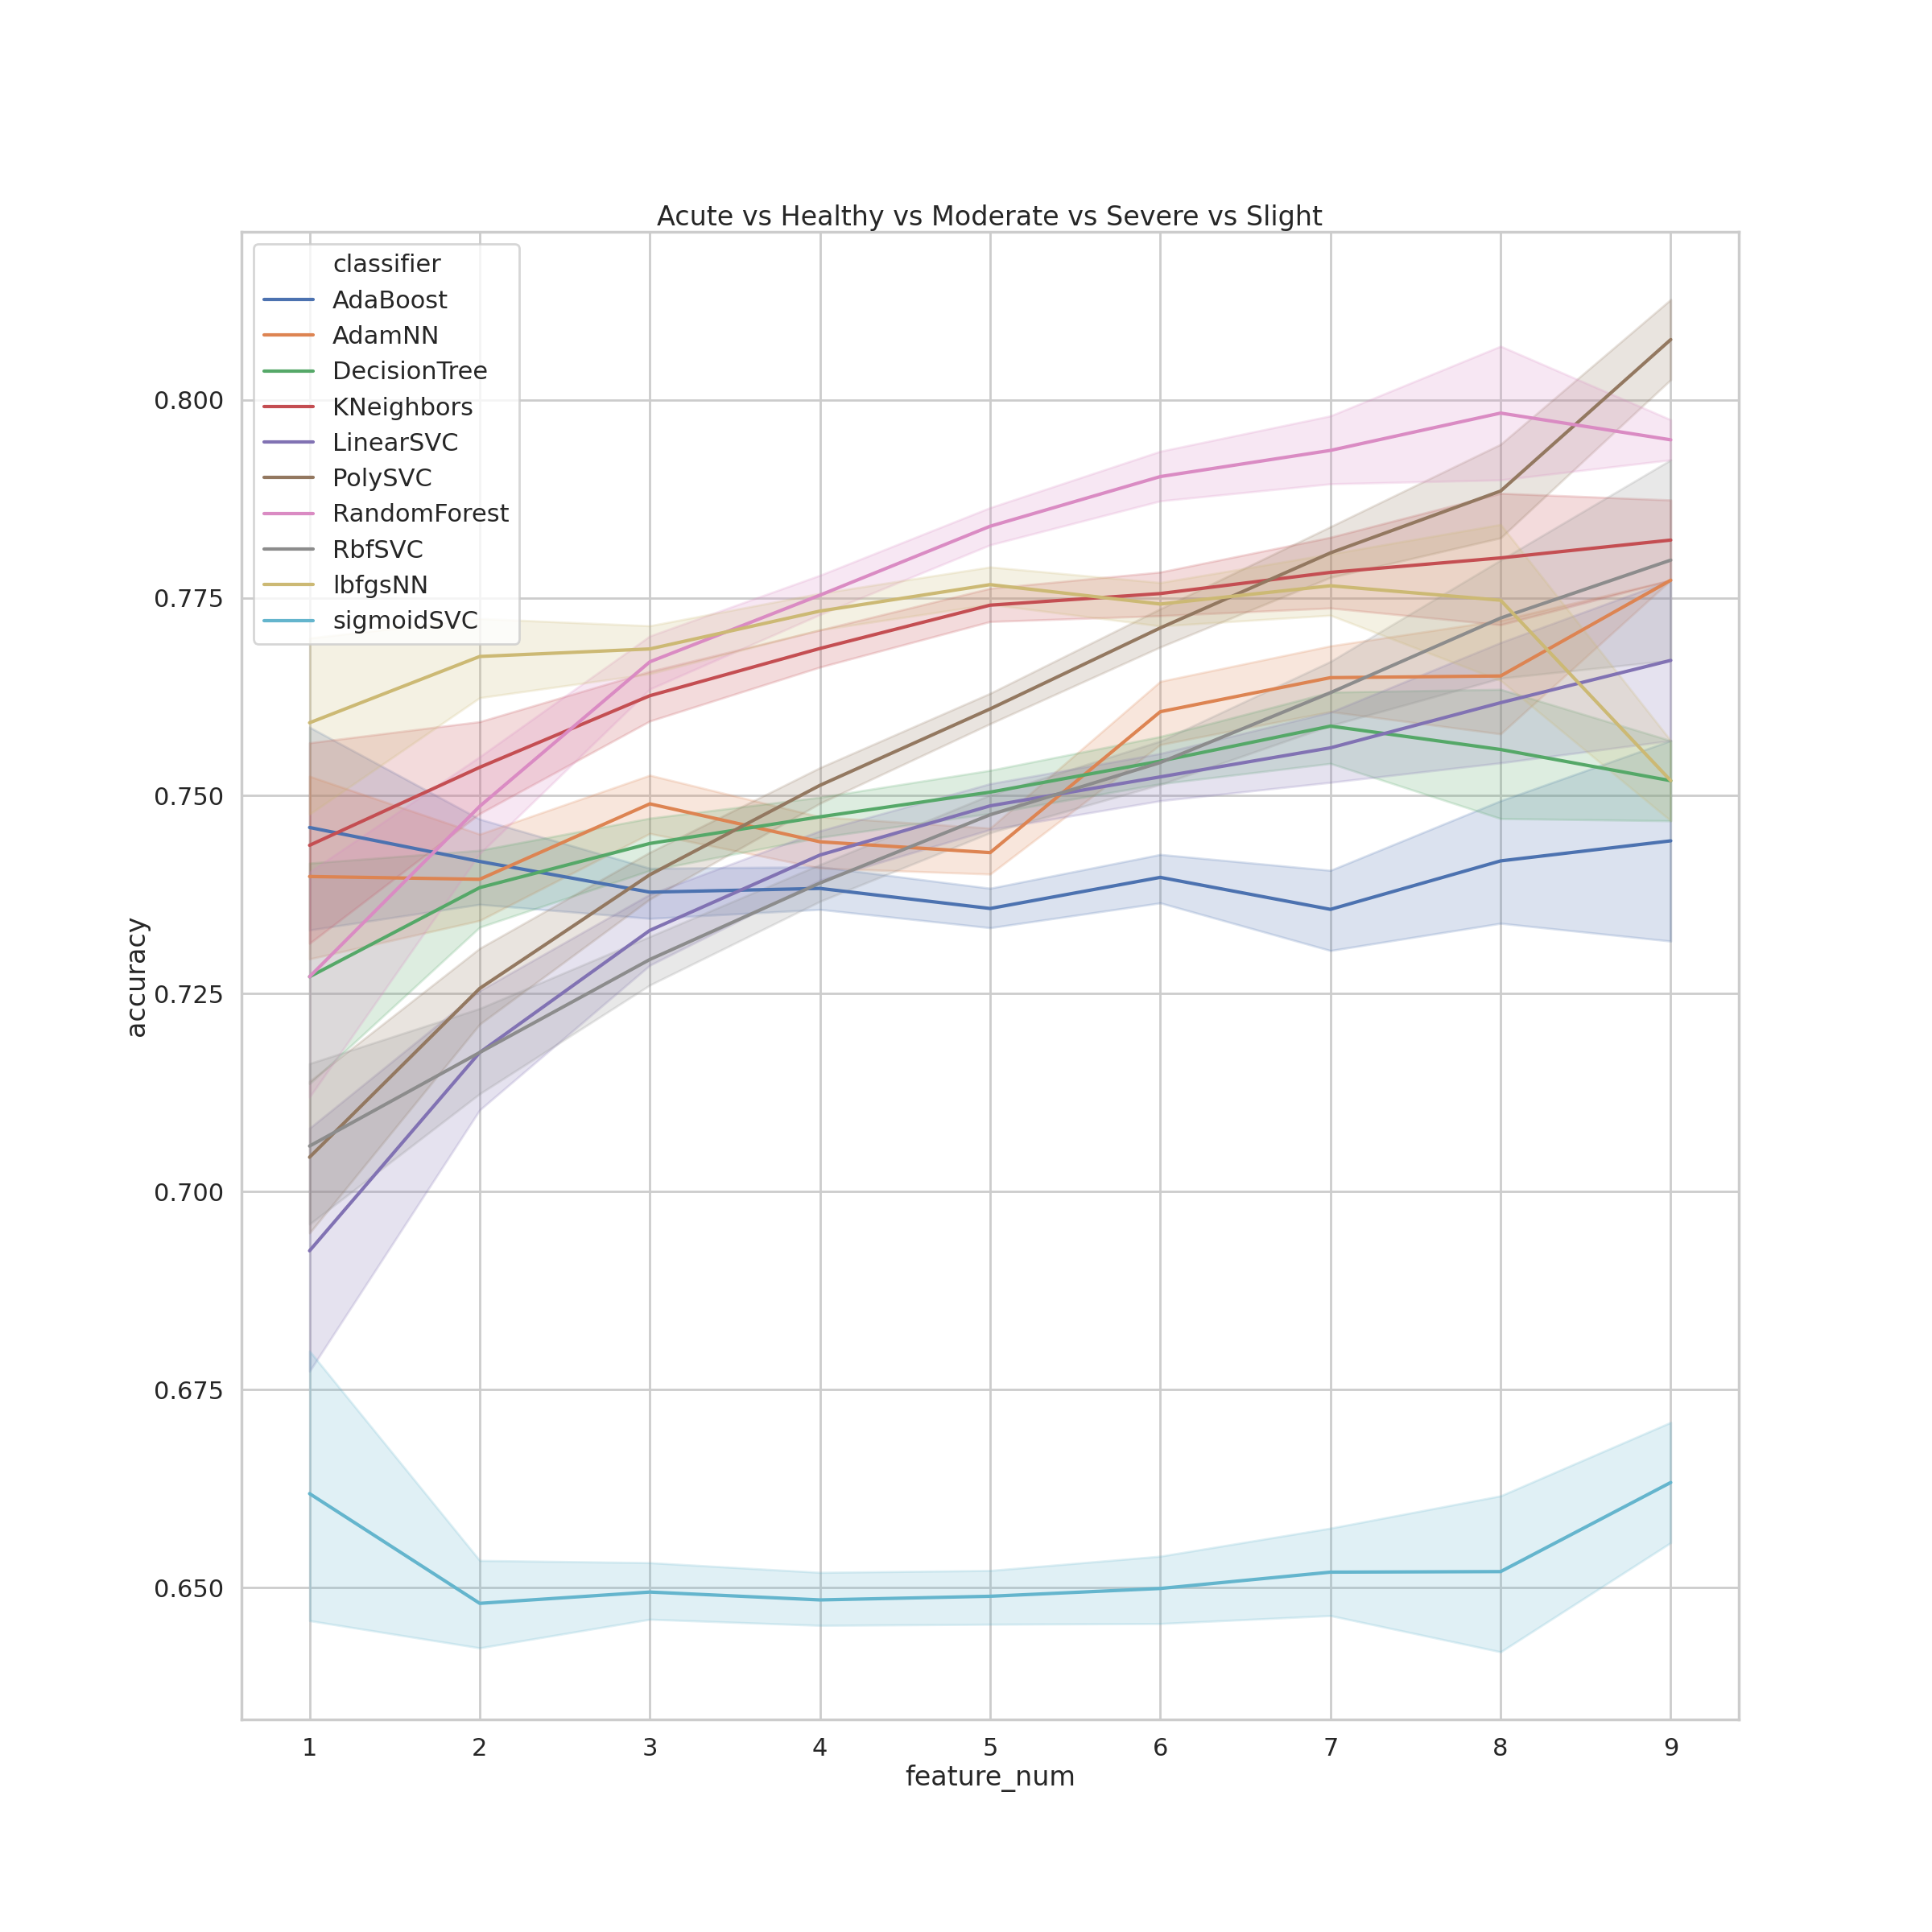
\includegraphics[width=0.3 \linewidth]{figures/5-class/accuracy.png}
					&
					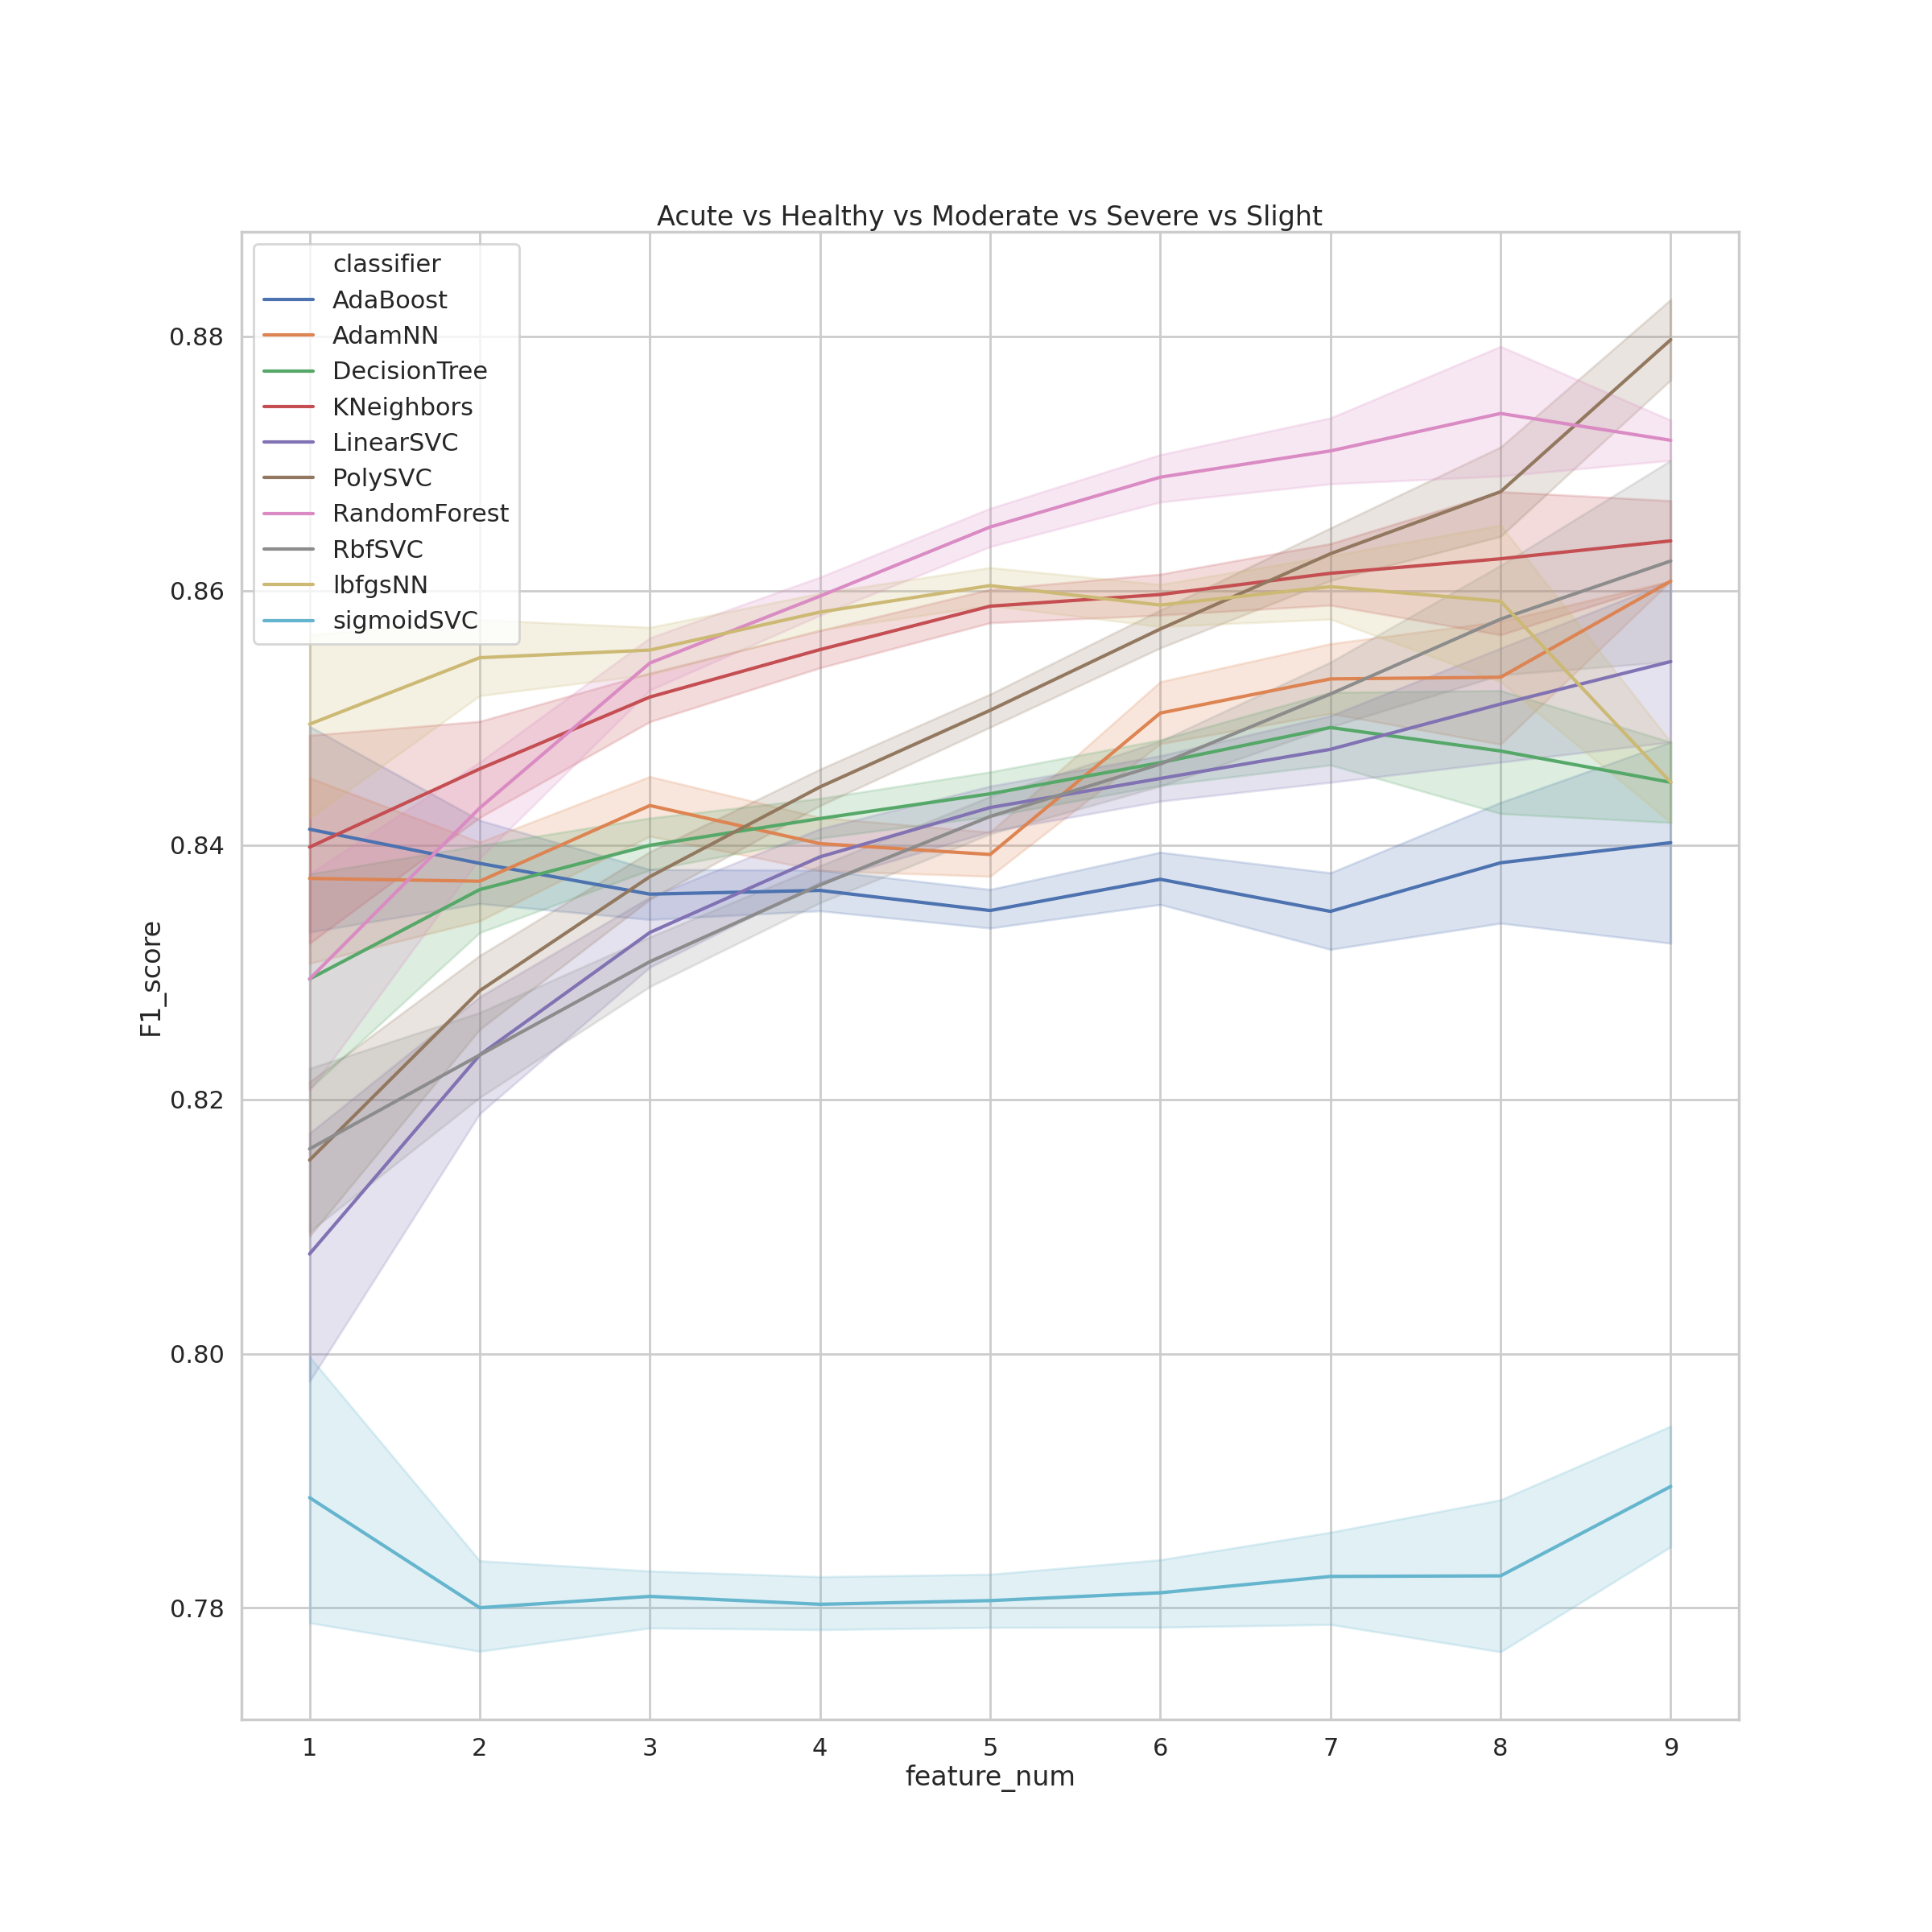
\includegraphics[width=0.3 \linewidth]{figures/5-class/F1_score.png}
					&
					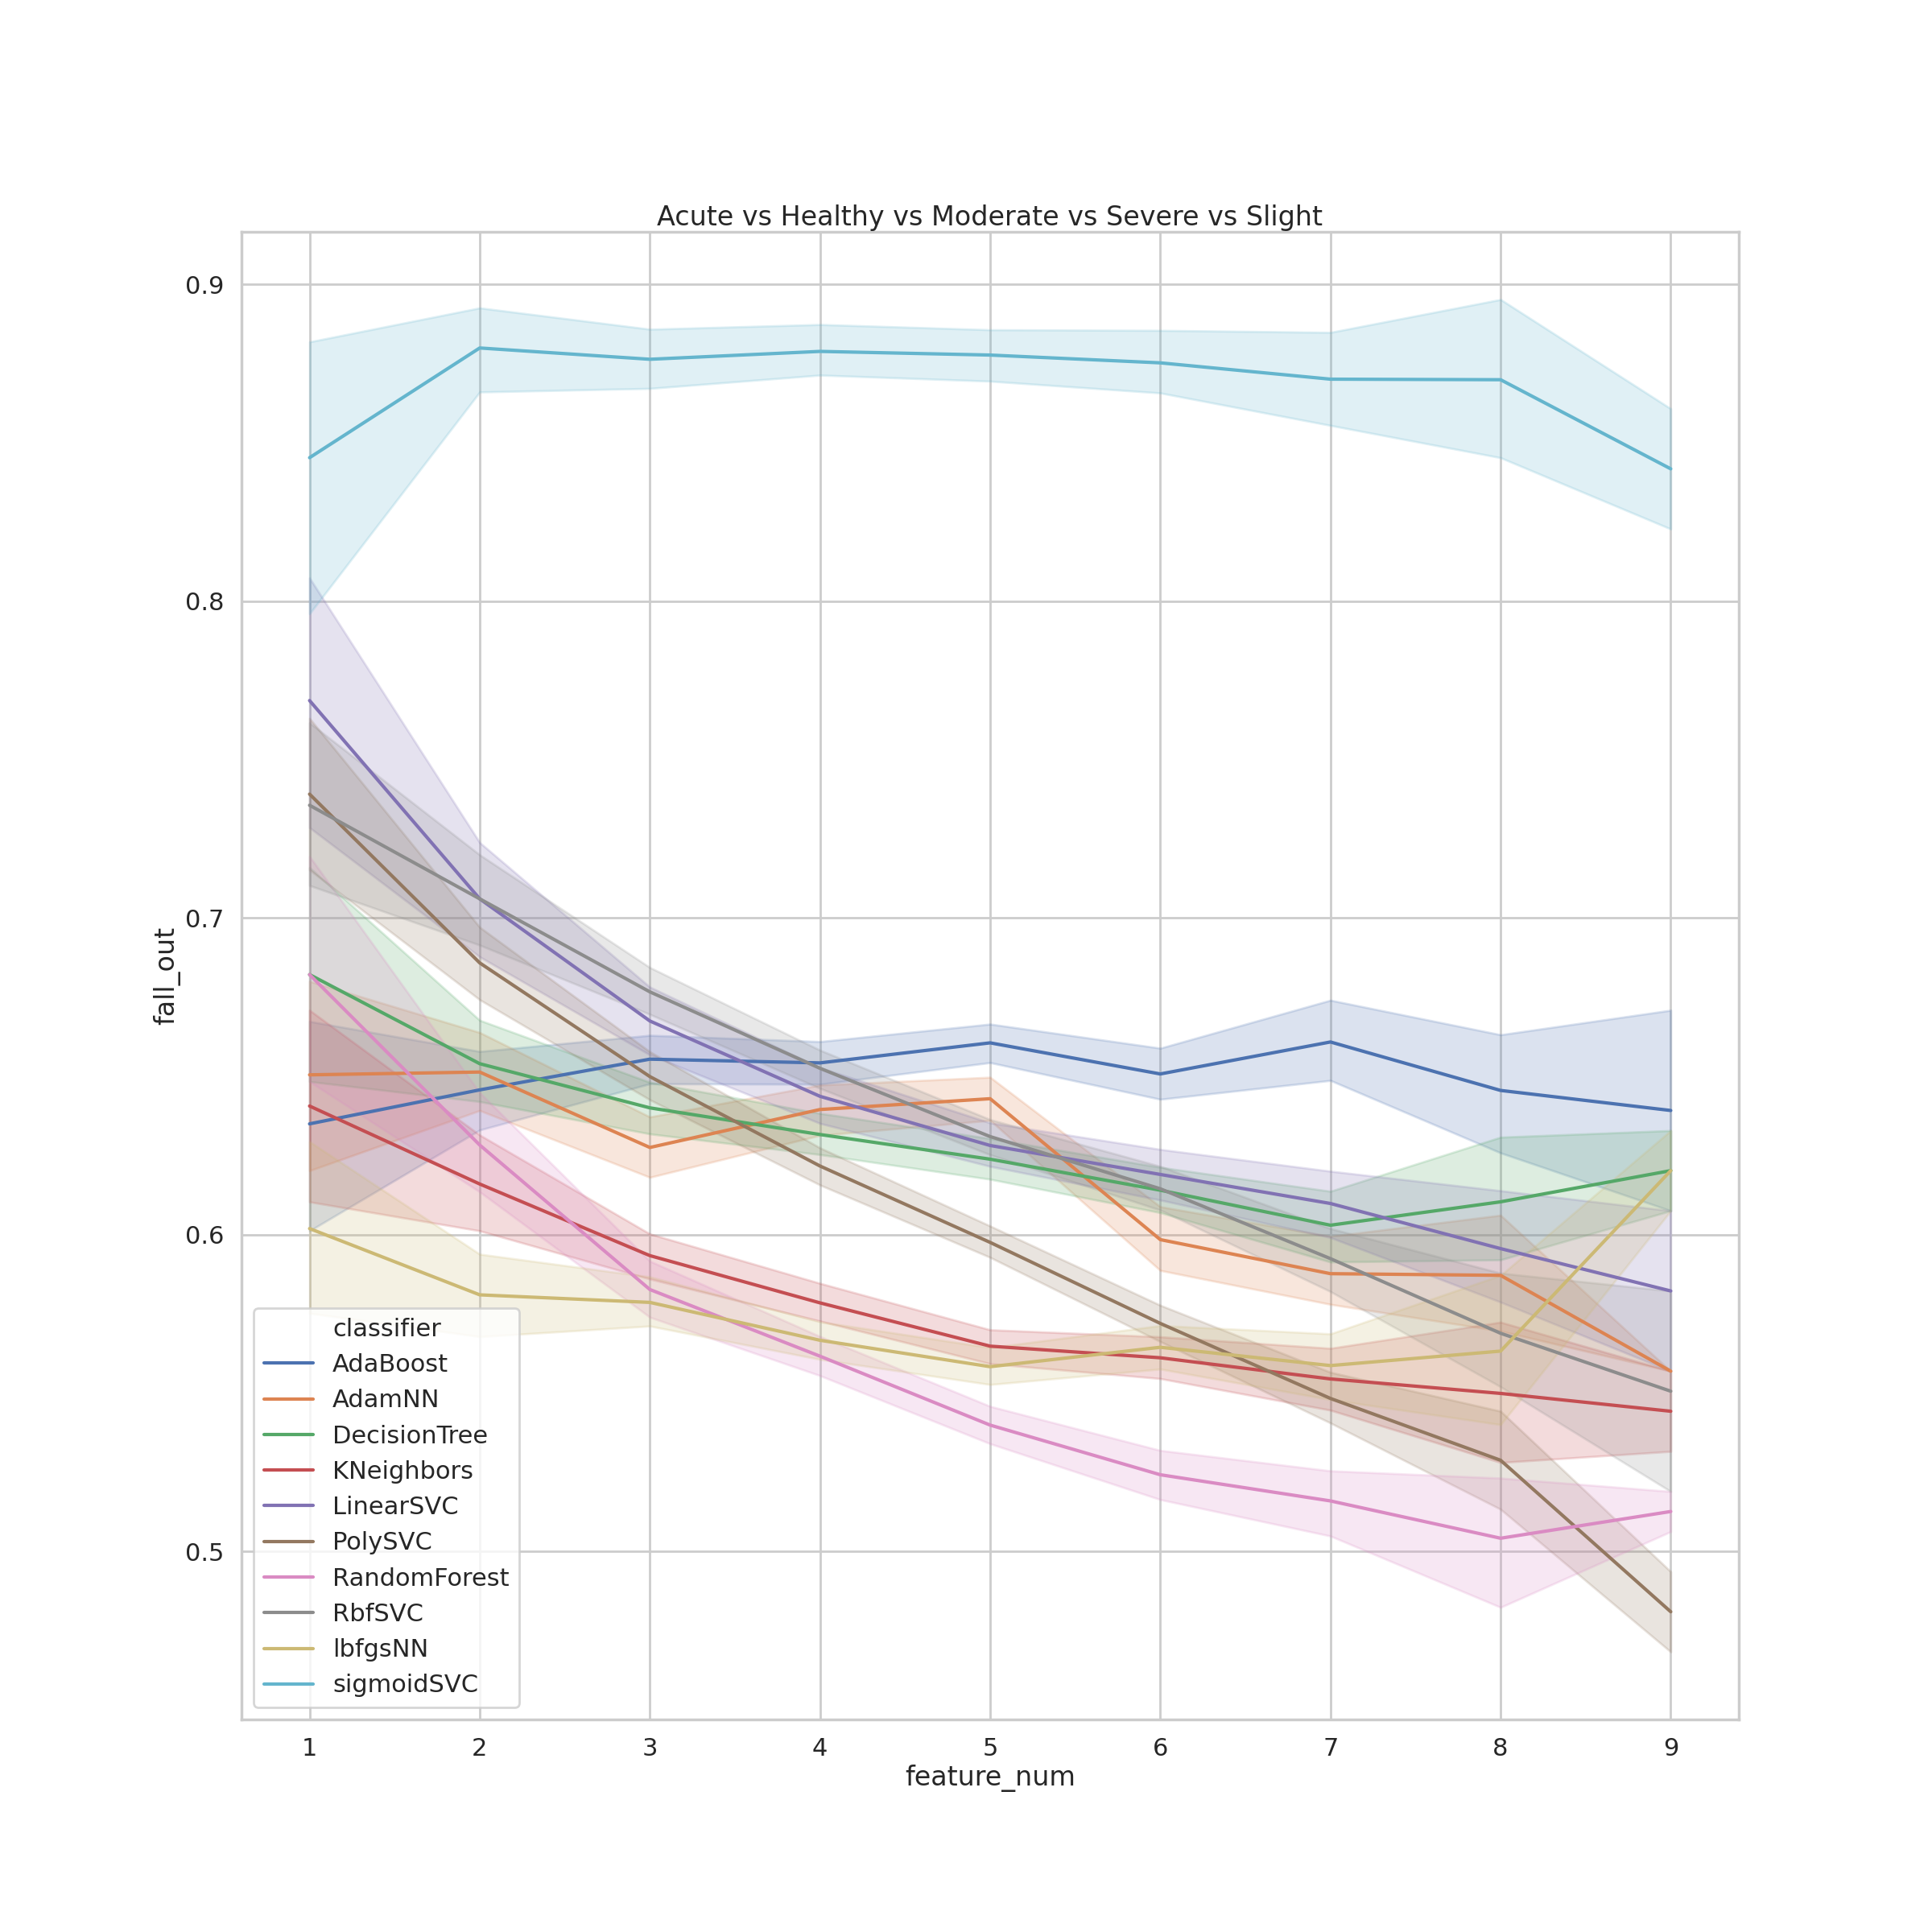
\includegraphics[width=0.3 \linewidth]{figures/5-class/fall_out.png}
					\\
					\mbox{Accuracy} & \mbox{F1 score} & \mbox{Fall-out} \\
					
					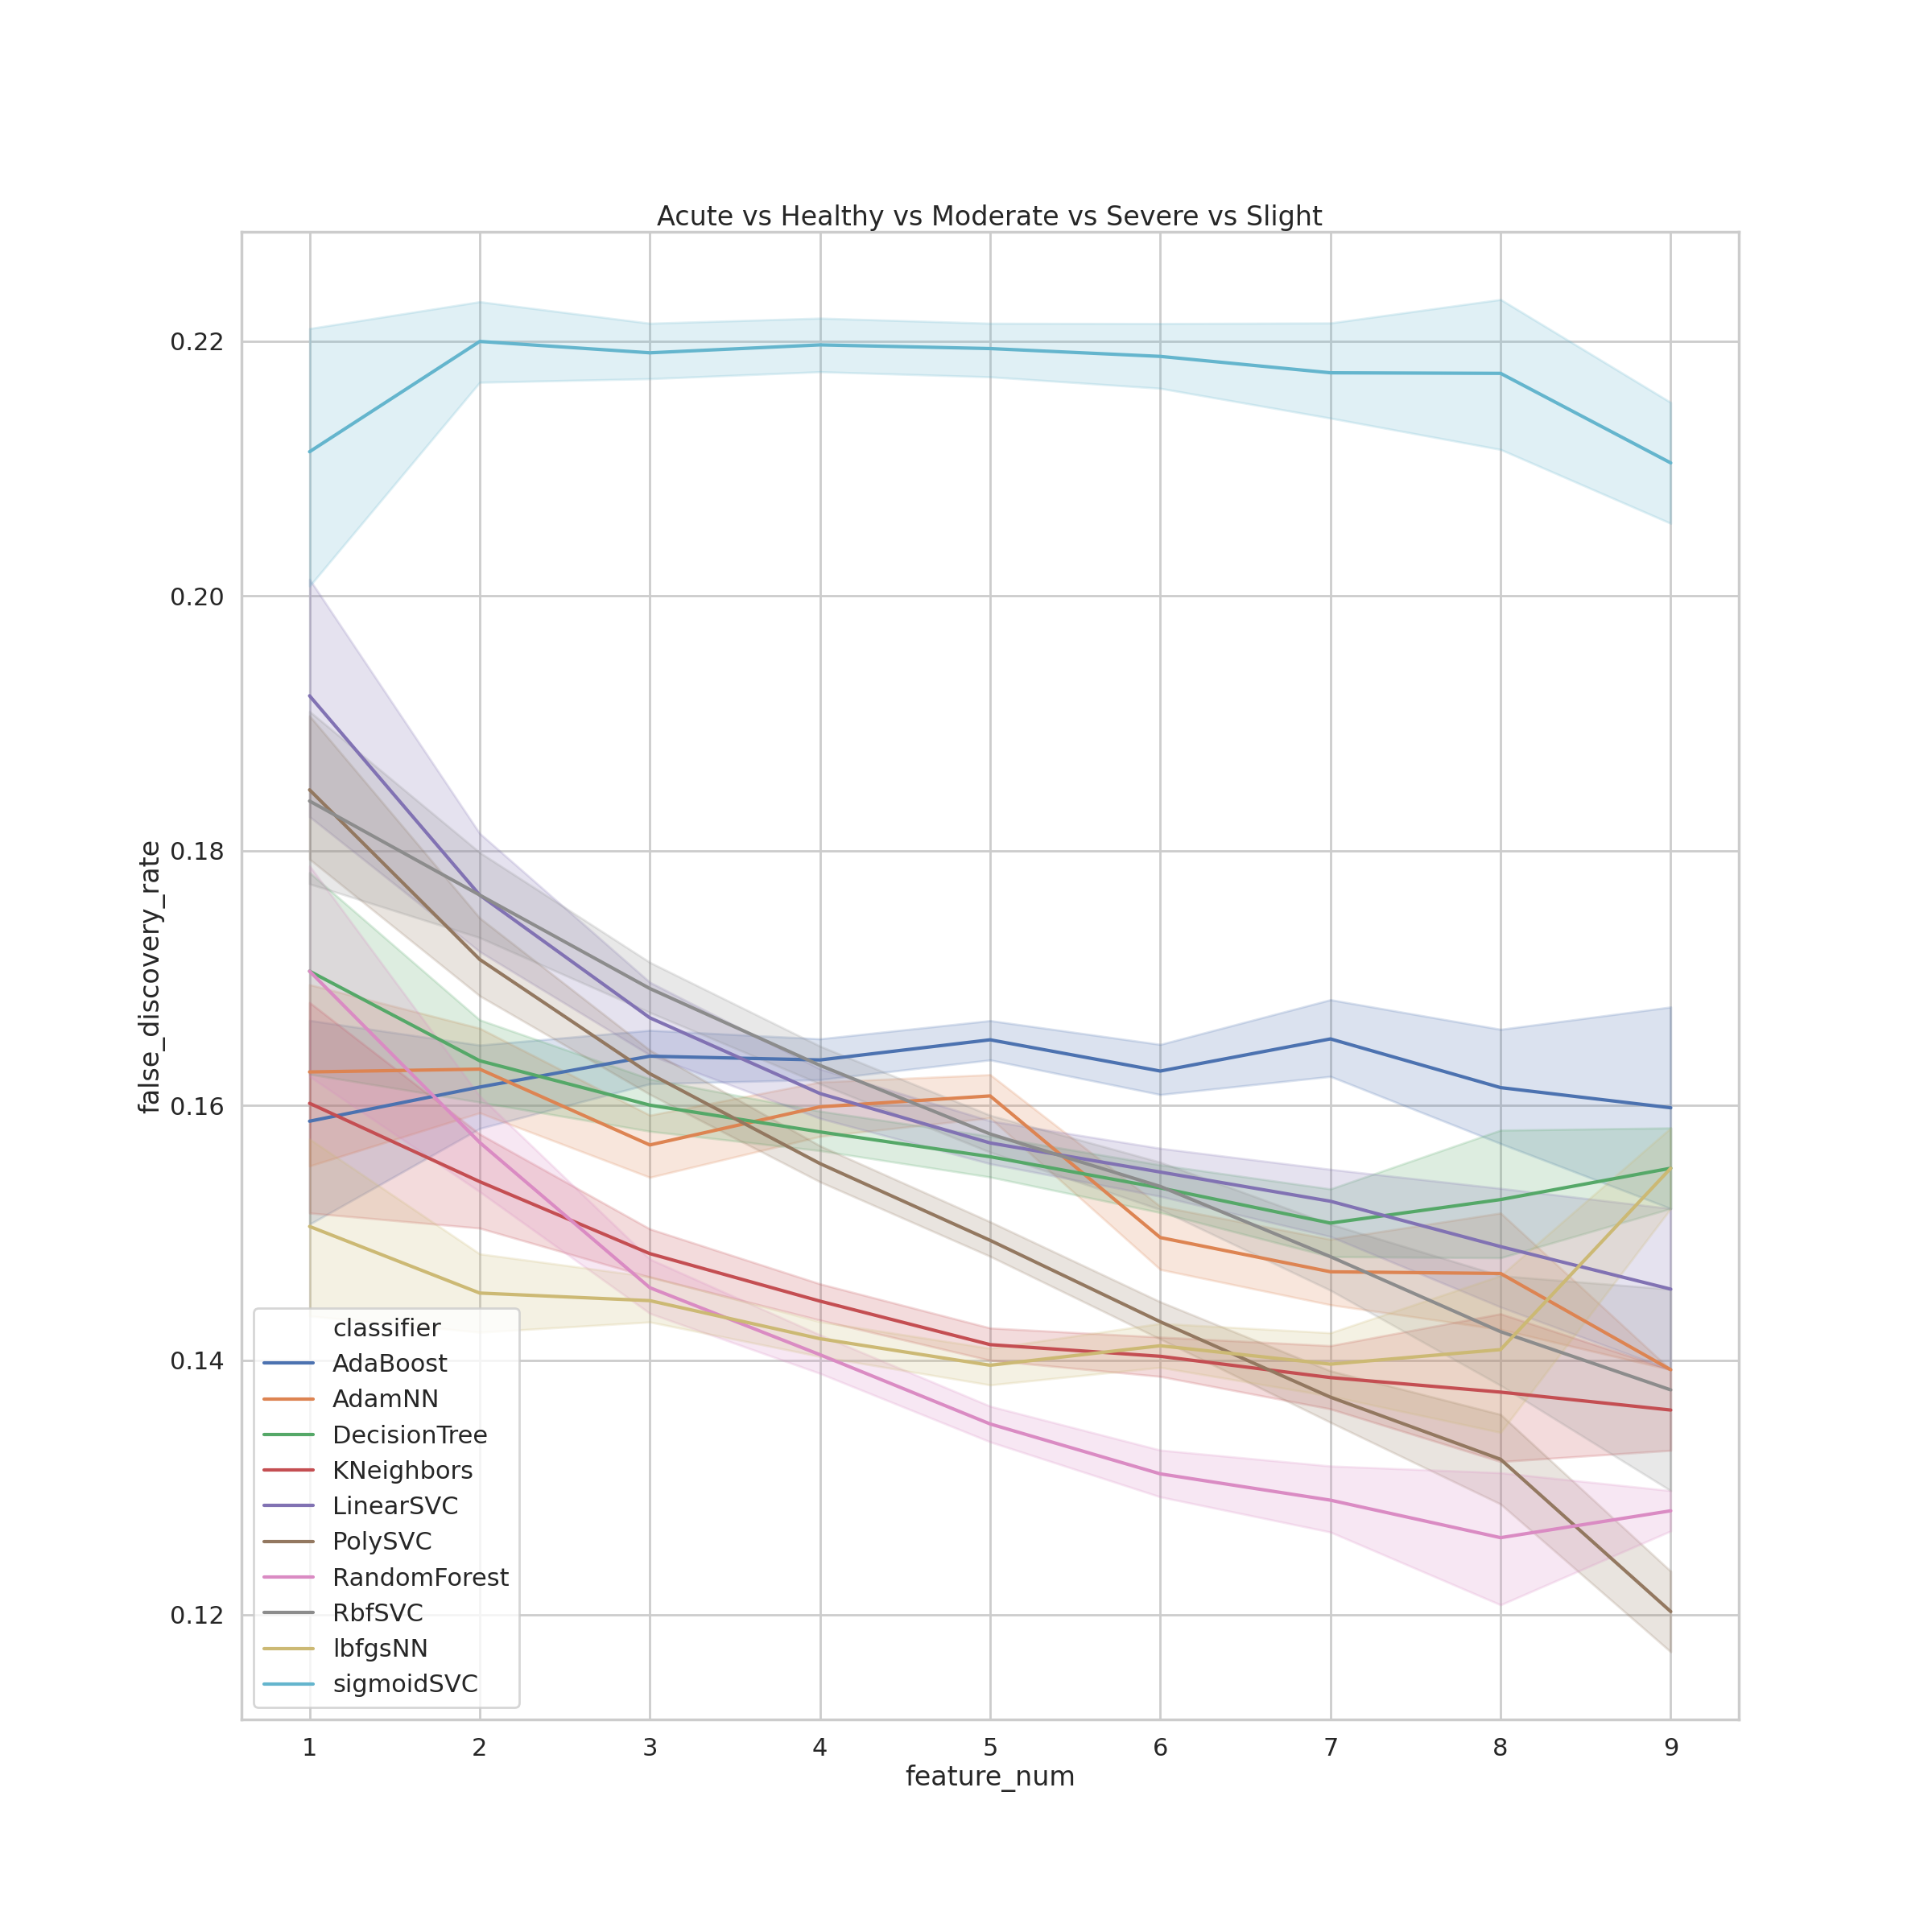
\includegraphics[width=0.3 \linewidth]{figures/5-class/false_discovery_rate.png}
					&
					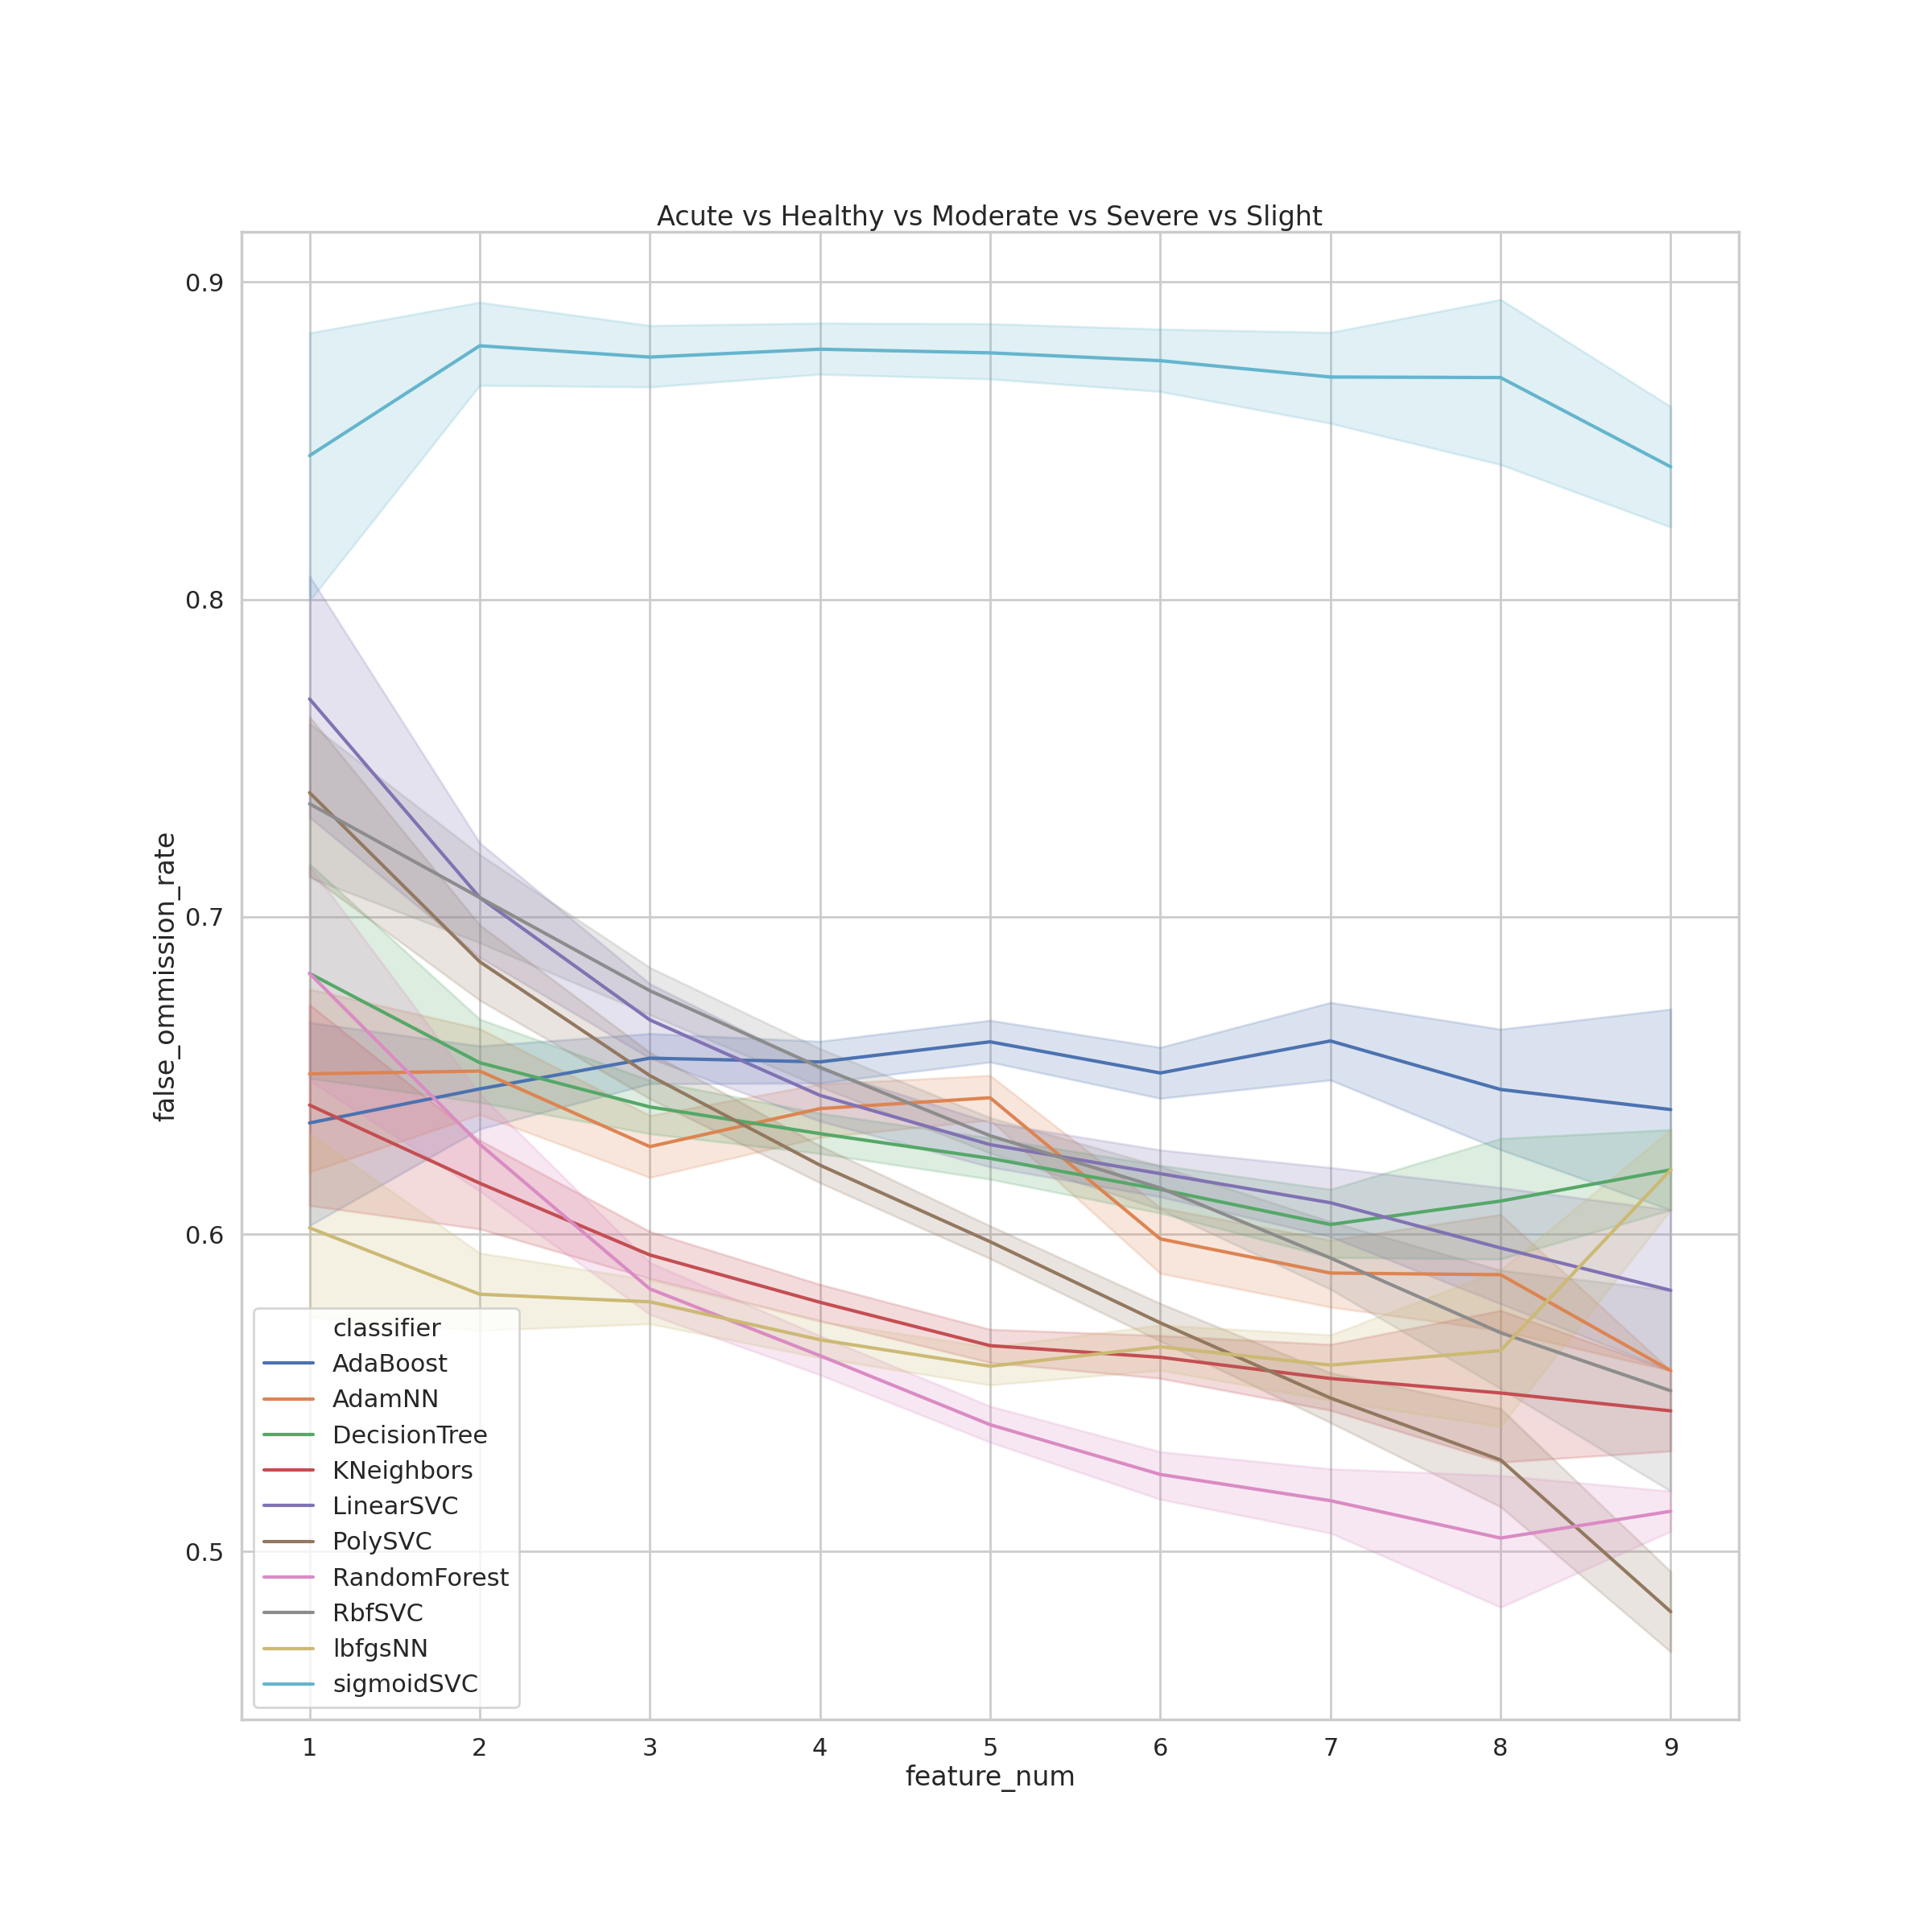
\includegraphics[width=0.3 \linewidth]{figures/5-class/false_ommission_rate.png}
					&
					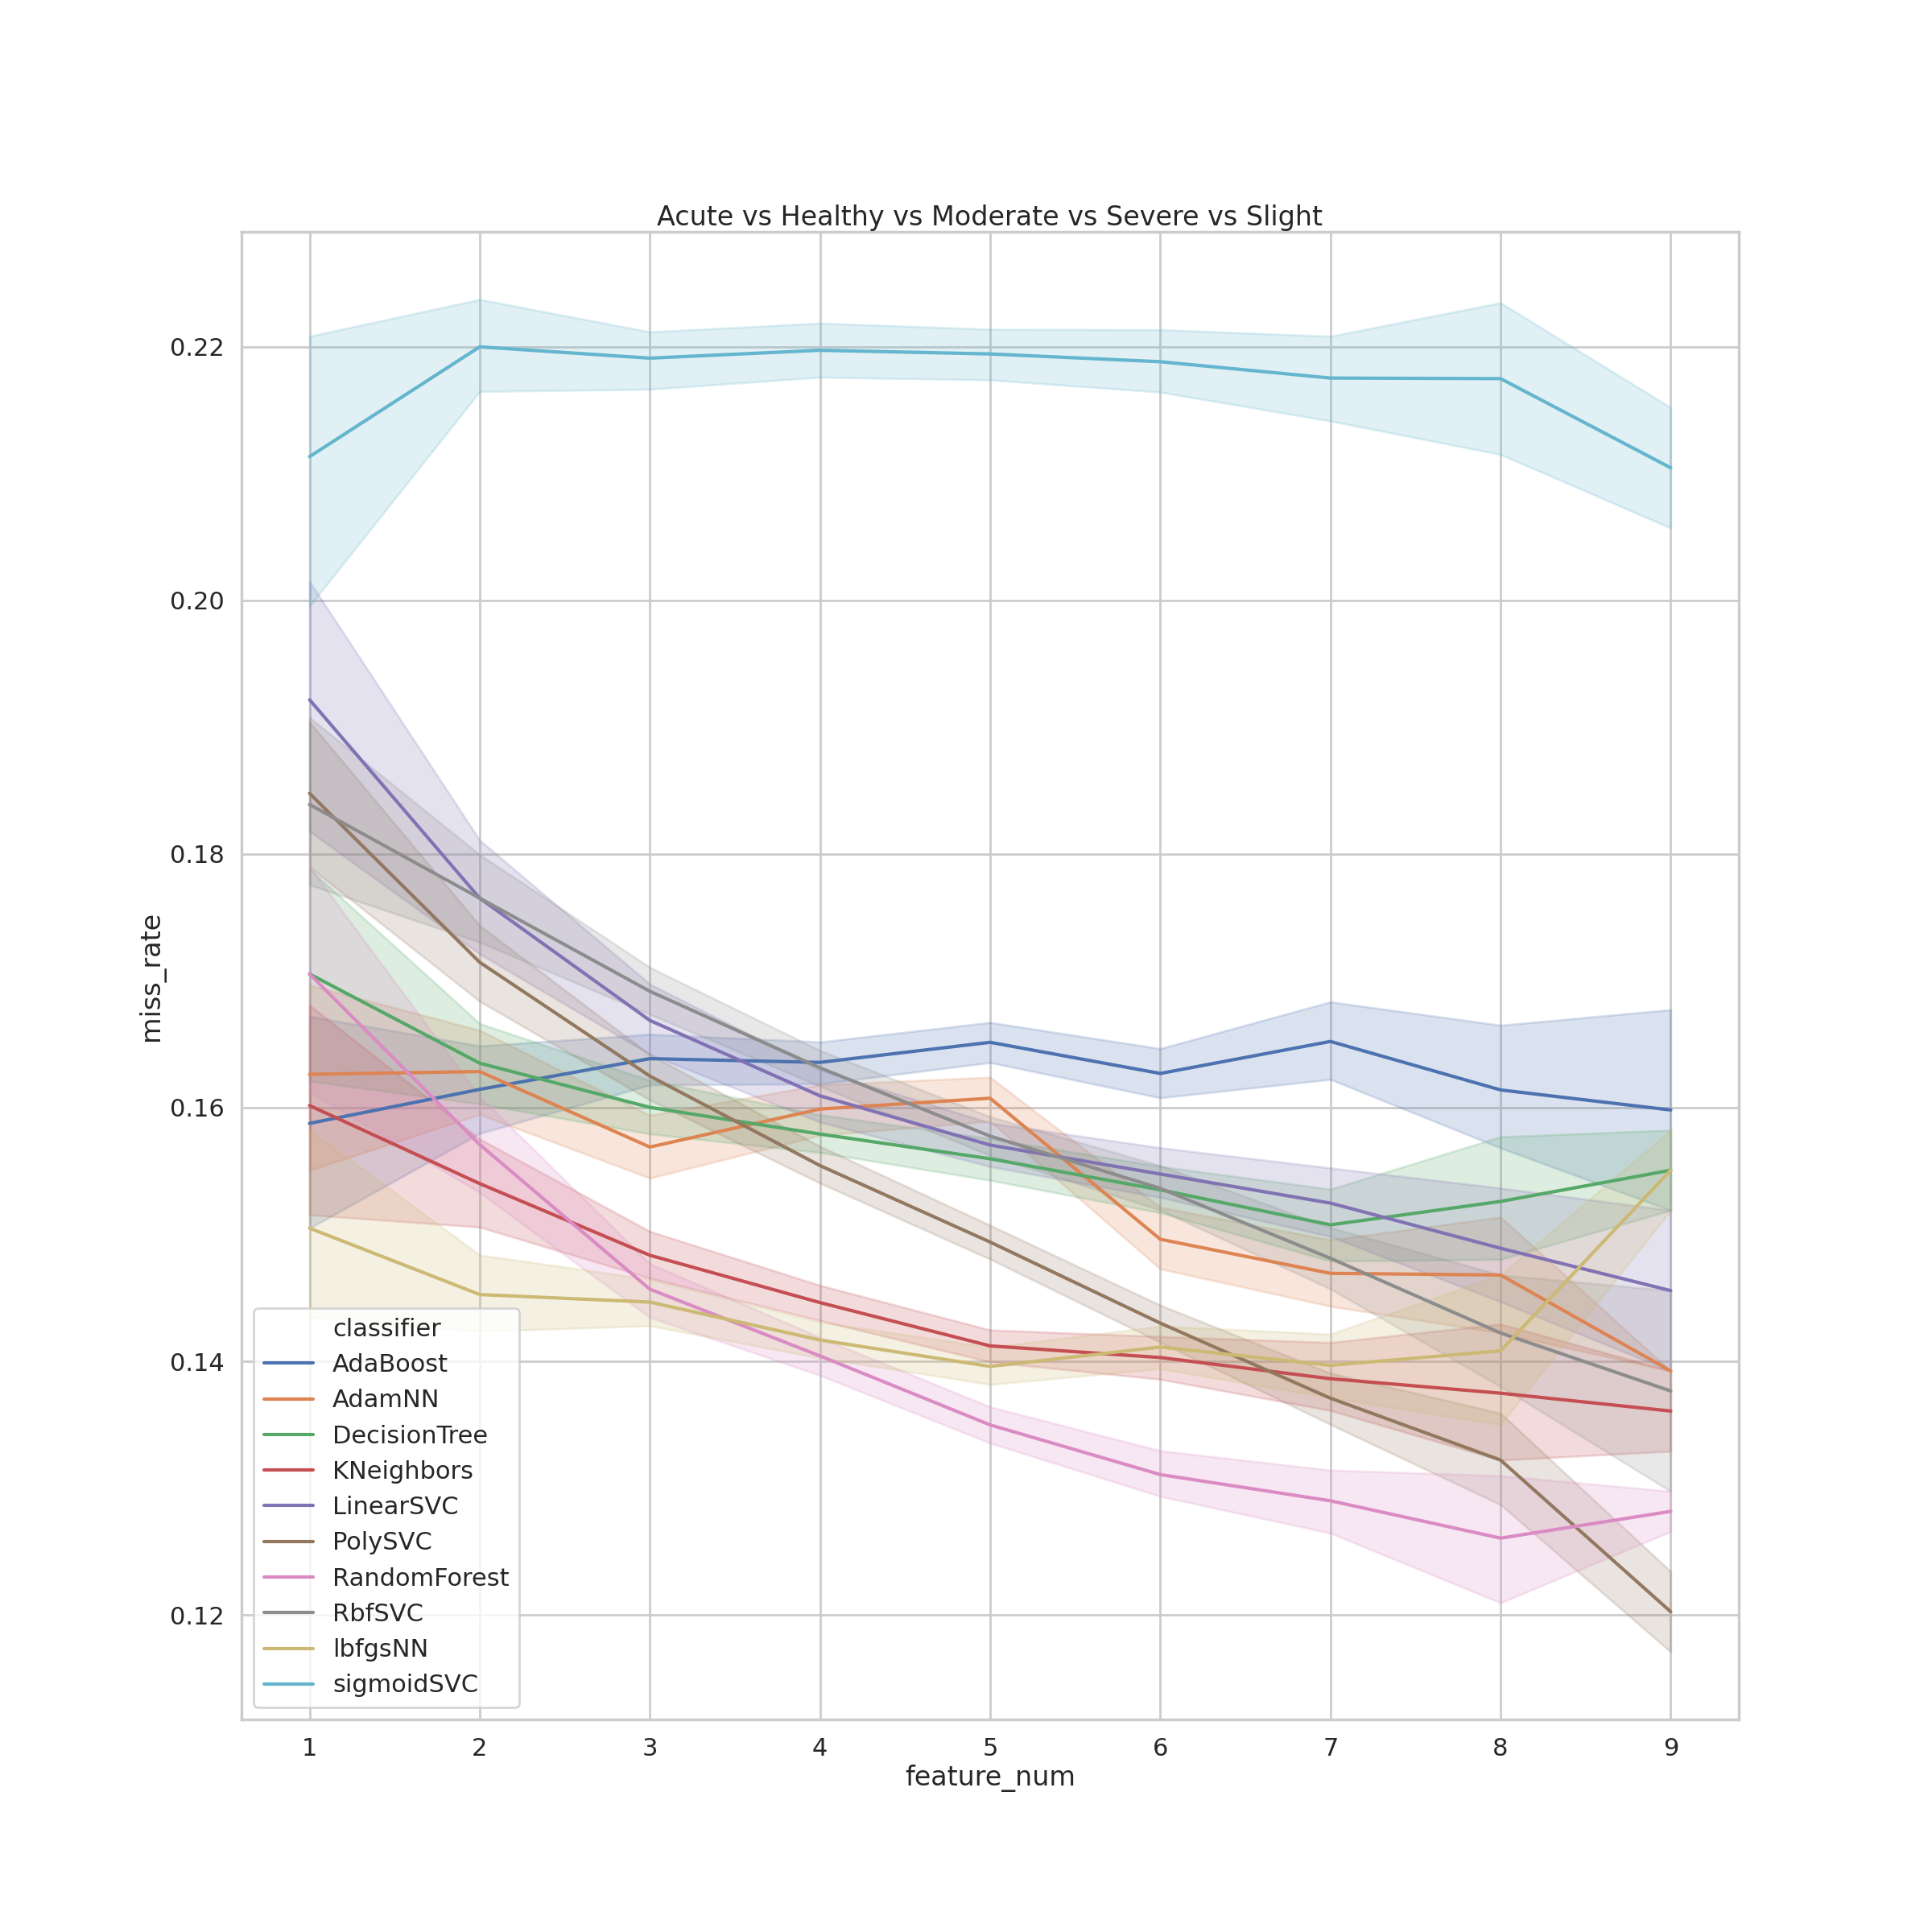
\includegraphics[width=0.3 \linewidth]{figures/5-class/miss_rate.png}
					\\
					\mbox{False discovery rate} & \mbox{False ommision rate} & \mbox{Miss rate} \\ 
					
					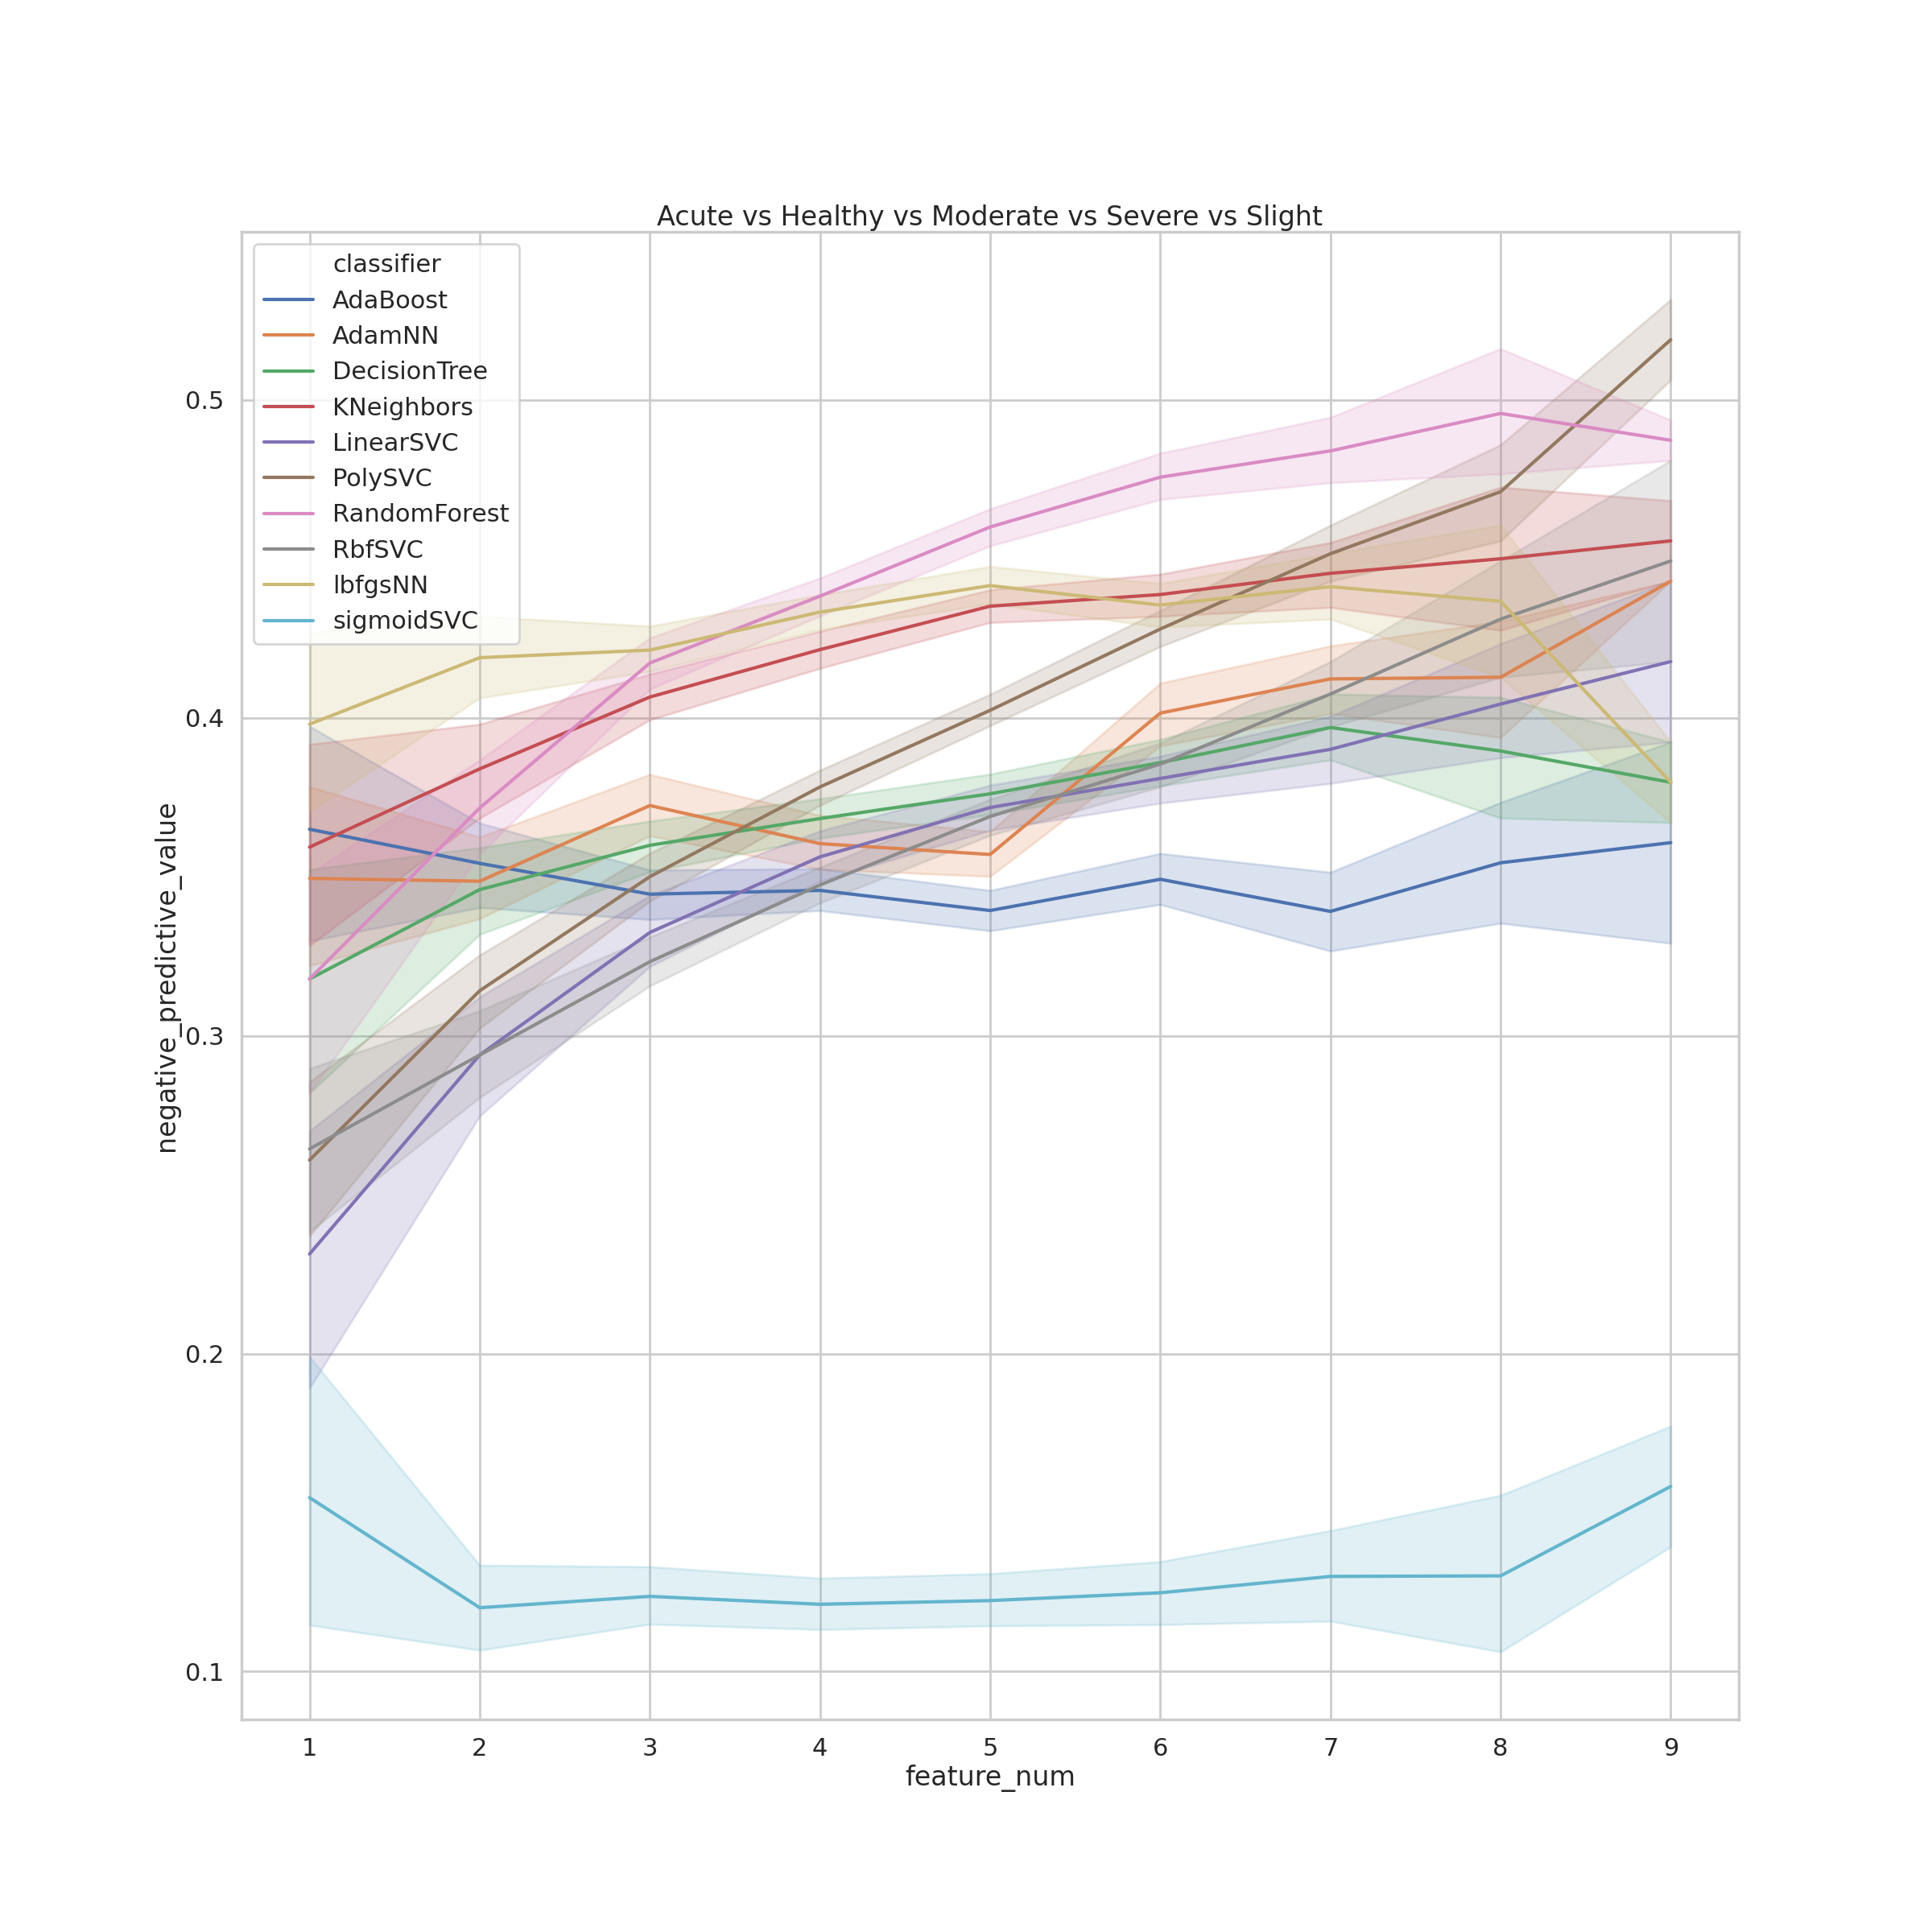
\includegraphics[width=0.3 \linewidth]{figures/5-class/negative_predictive_value.png}
					&
					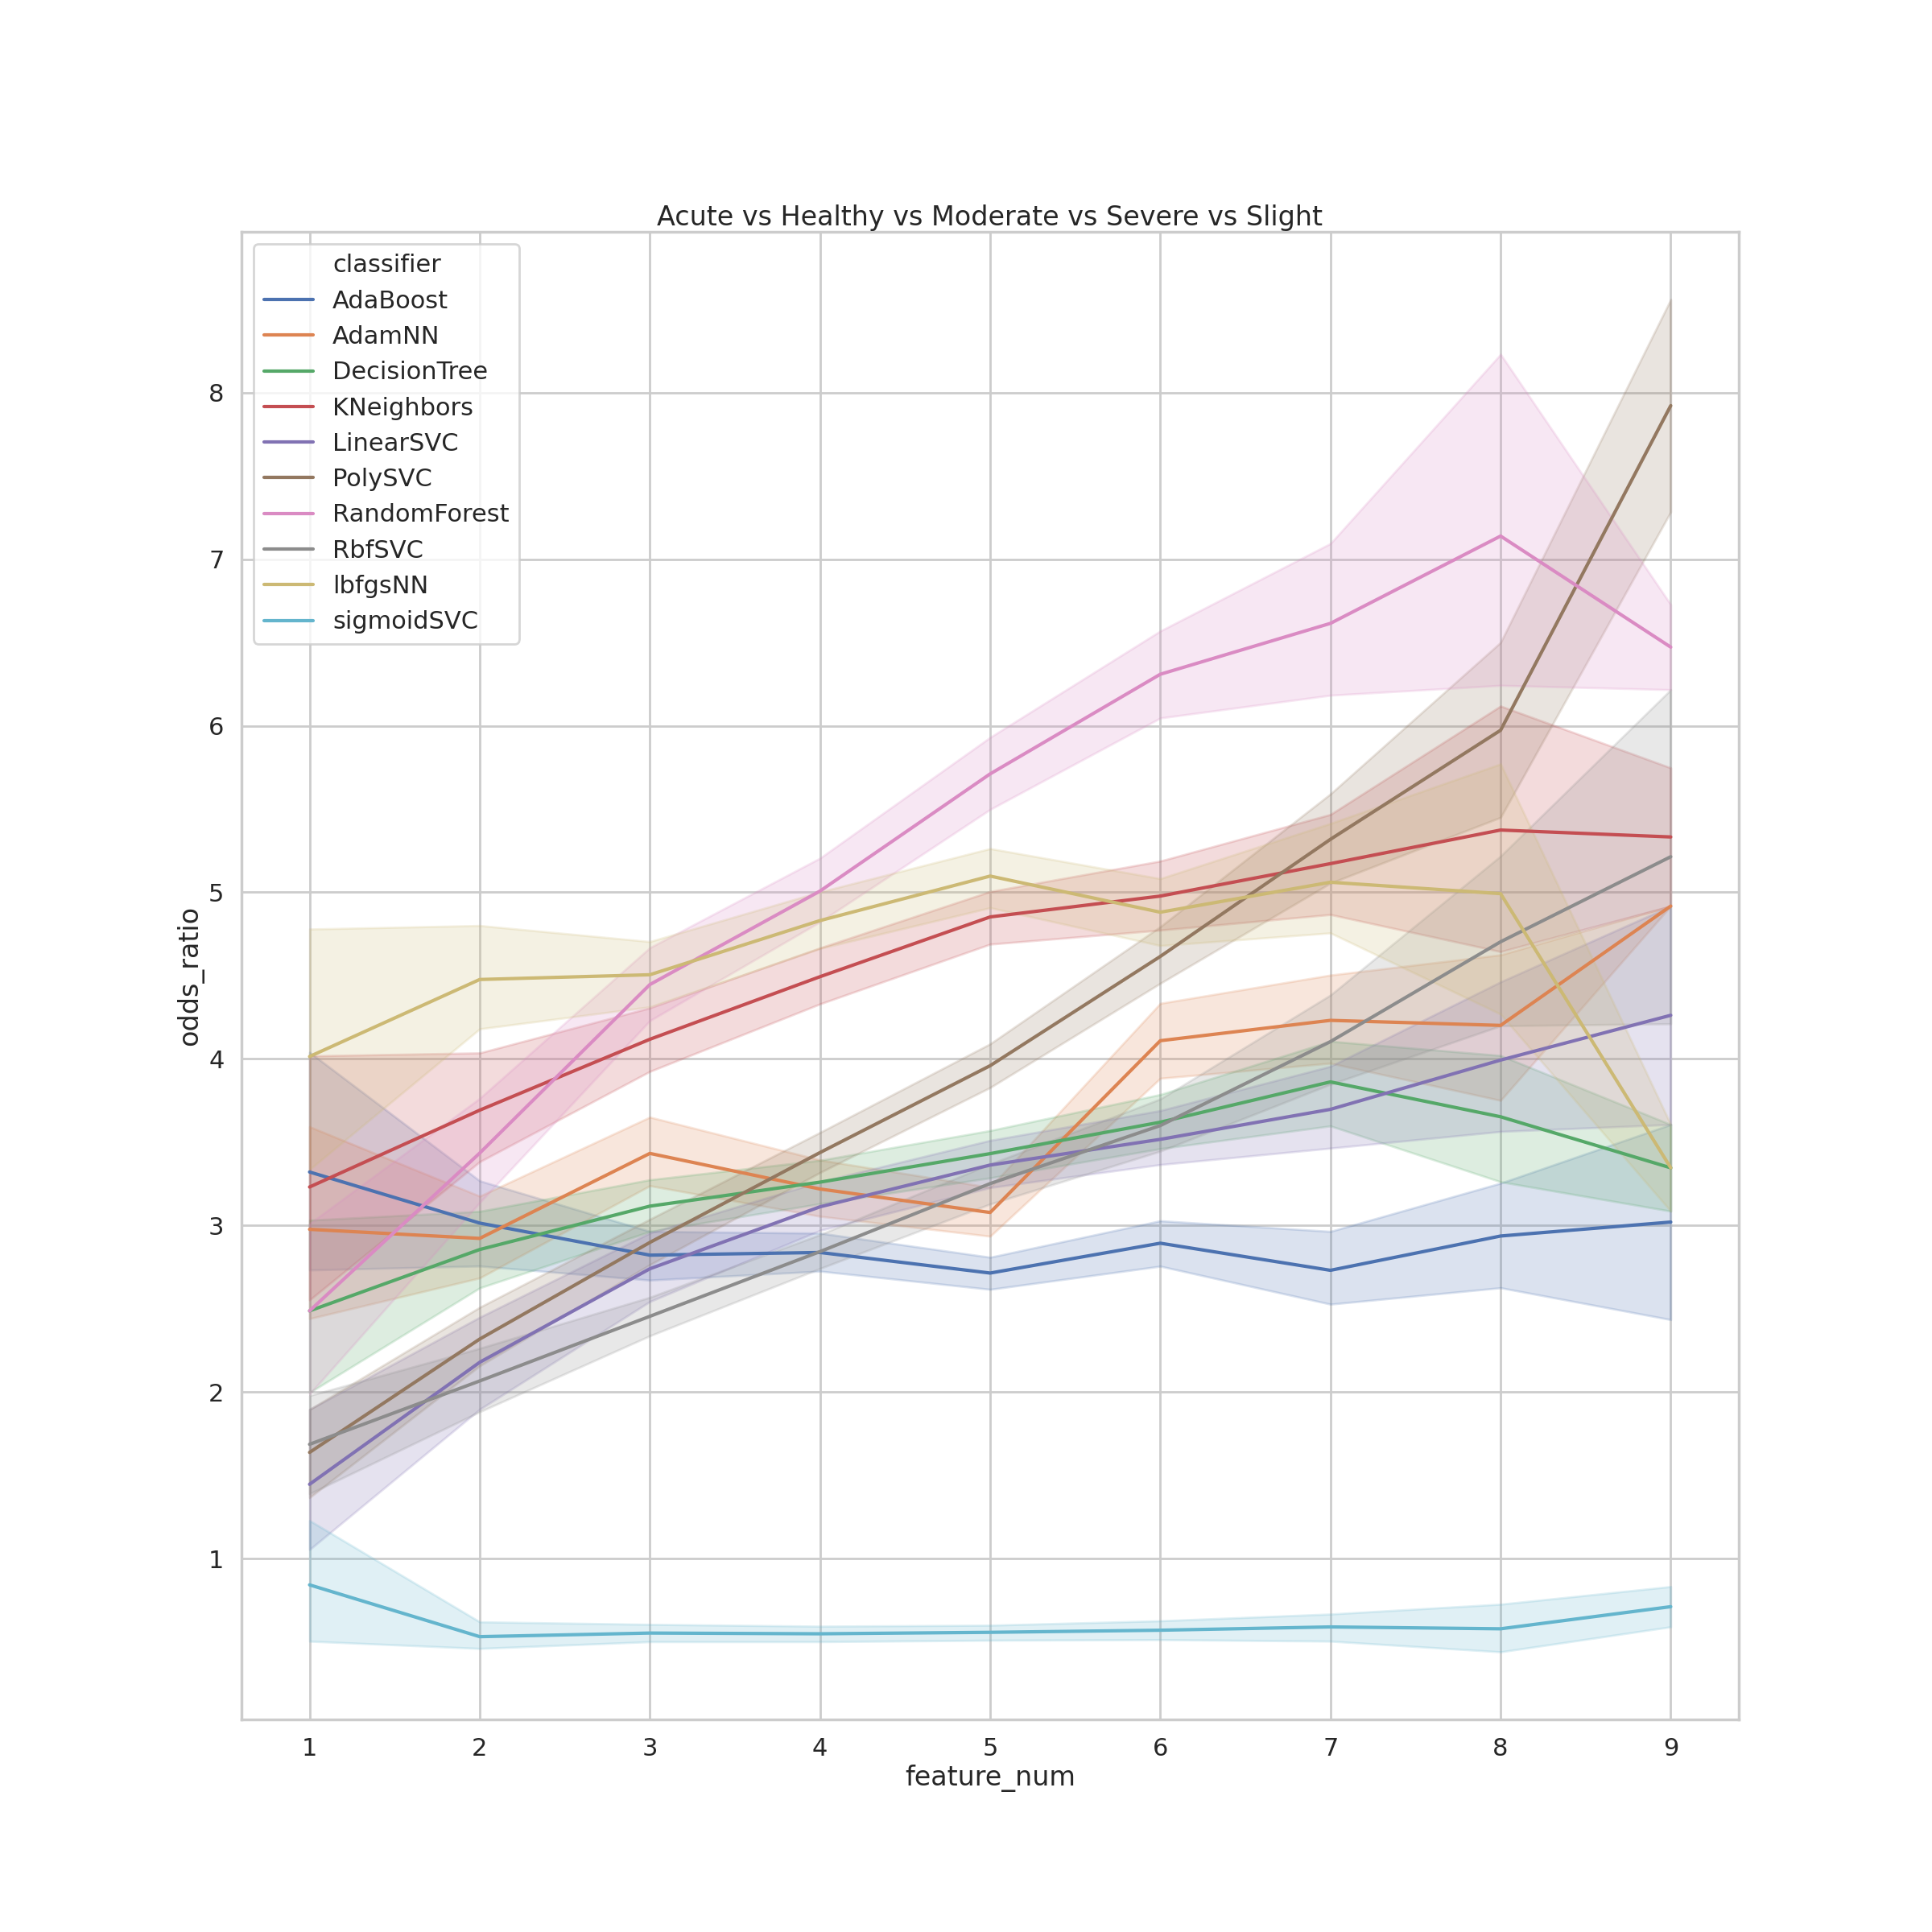
\includegraphics[width=0.3 \linewidth]{figures/5-class/odds_ratio.png}
					&
					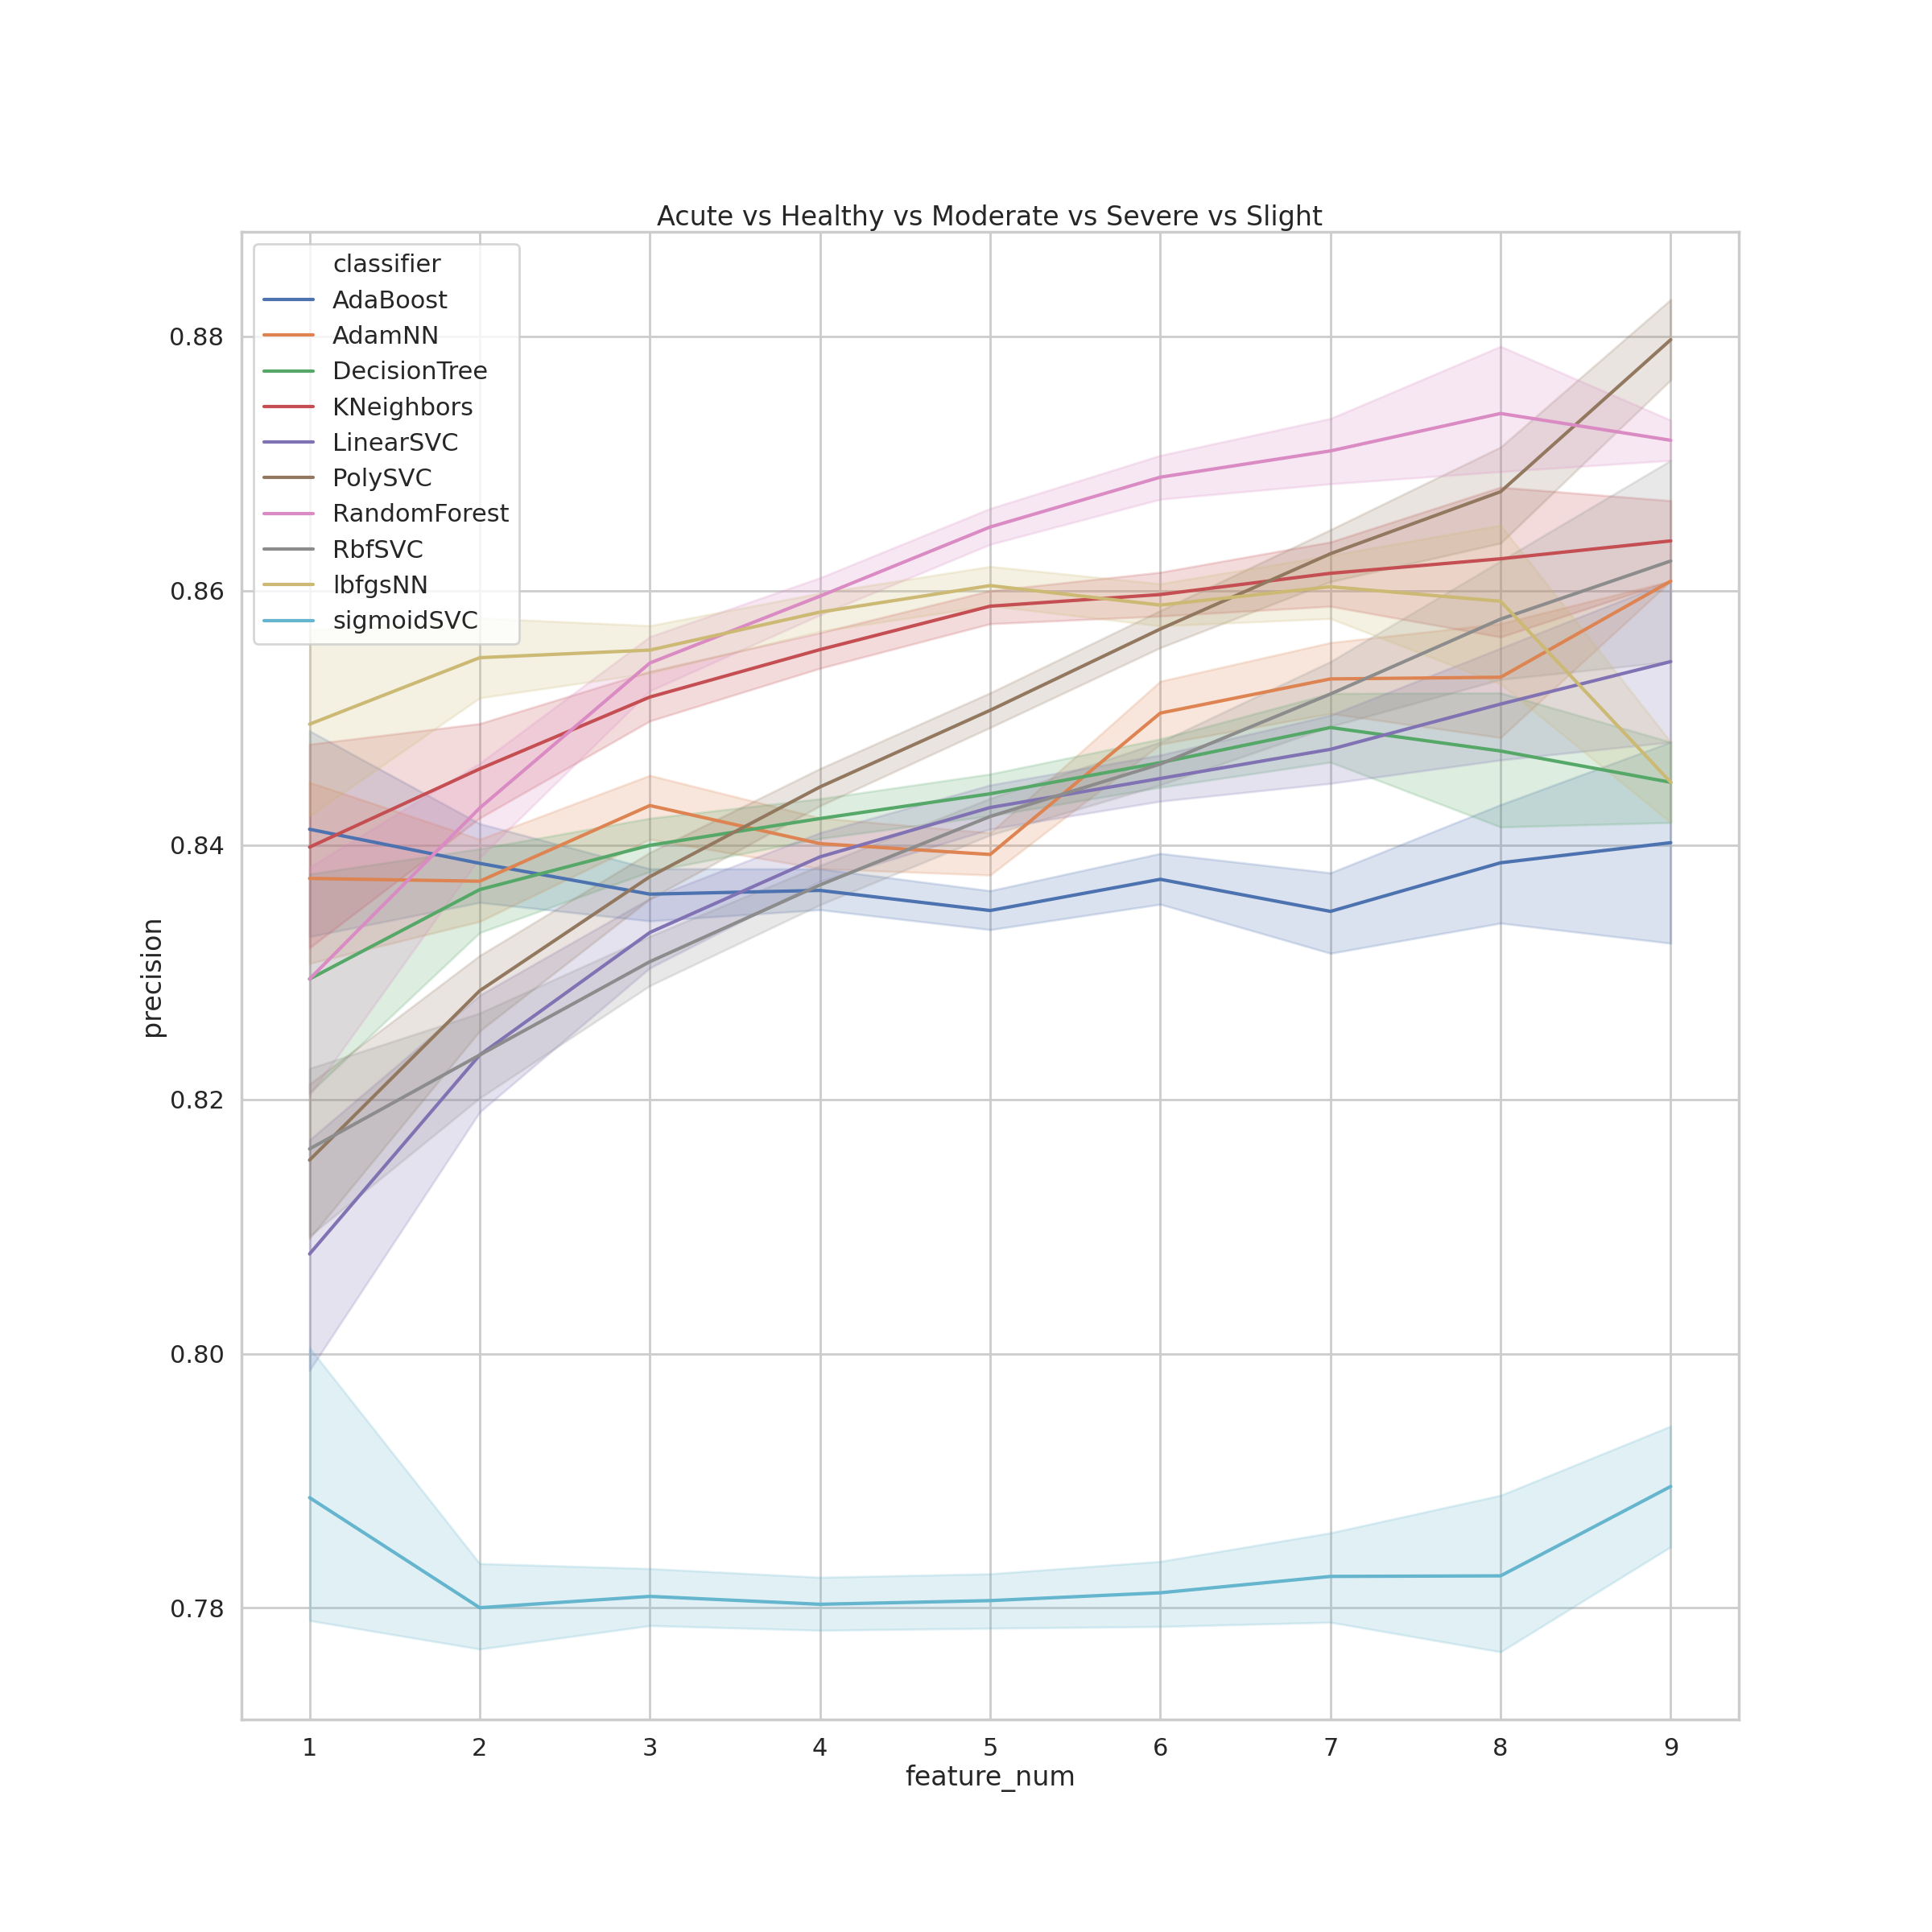
\includegraphics[width=0.3 \linewidth]{figures/5-class/precision.png}
					\\
					\mbox{Negative predictive value} & \mbox{Odds ratio} & \mbox{Precision} \\ 
					
					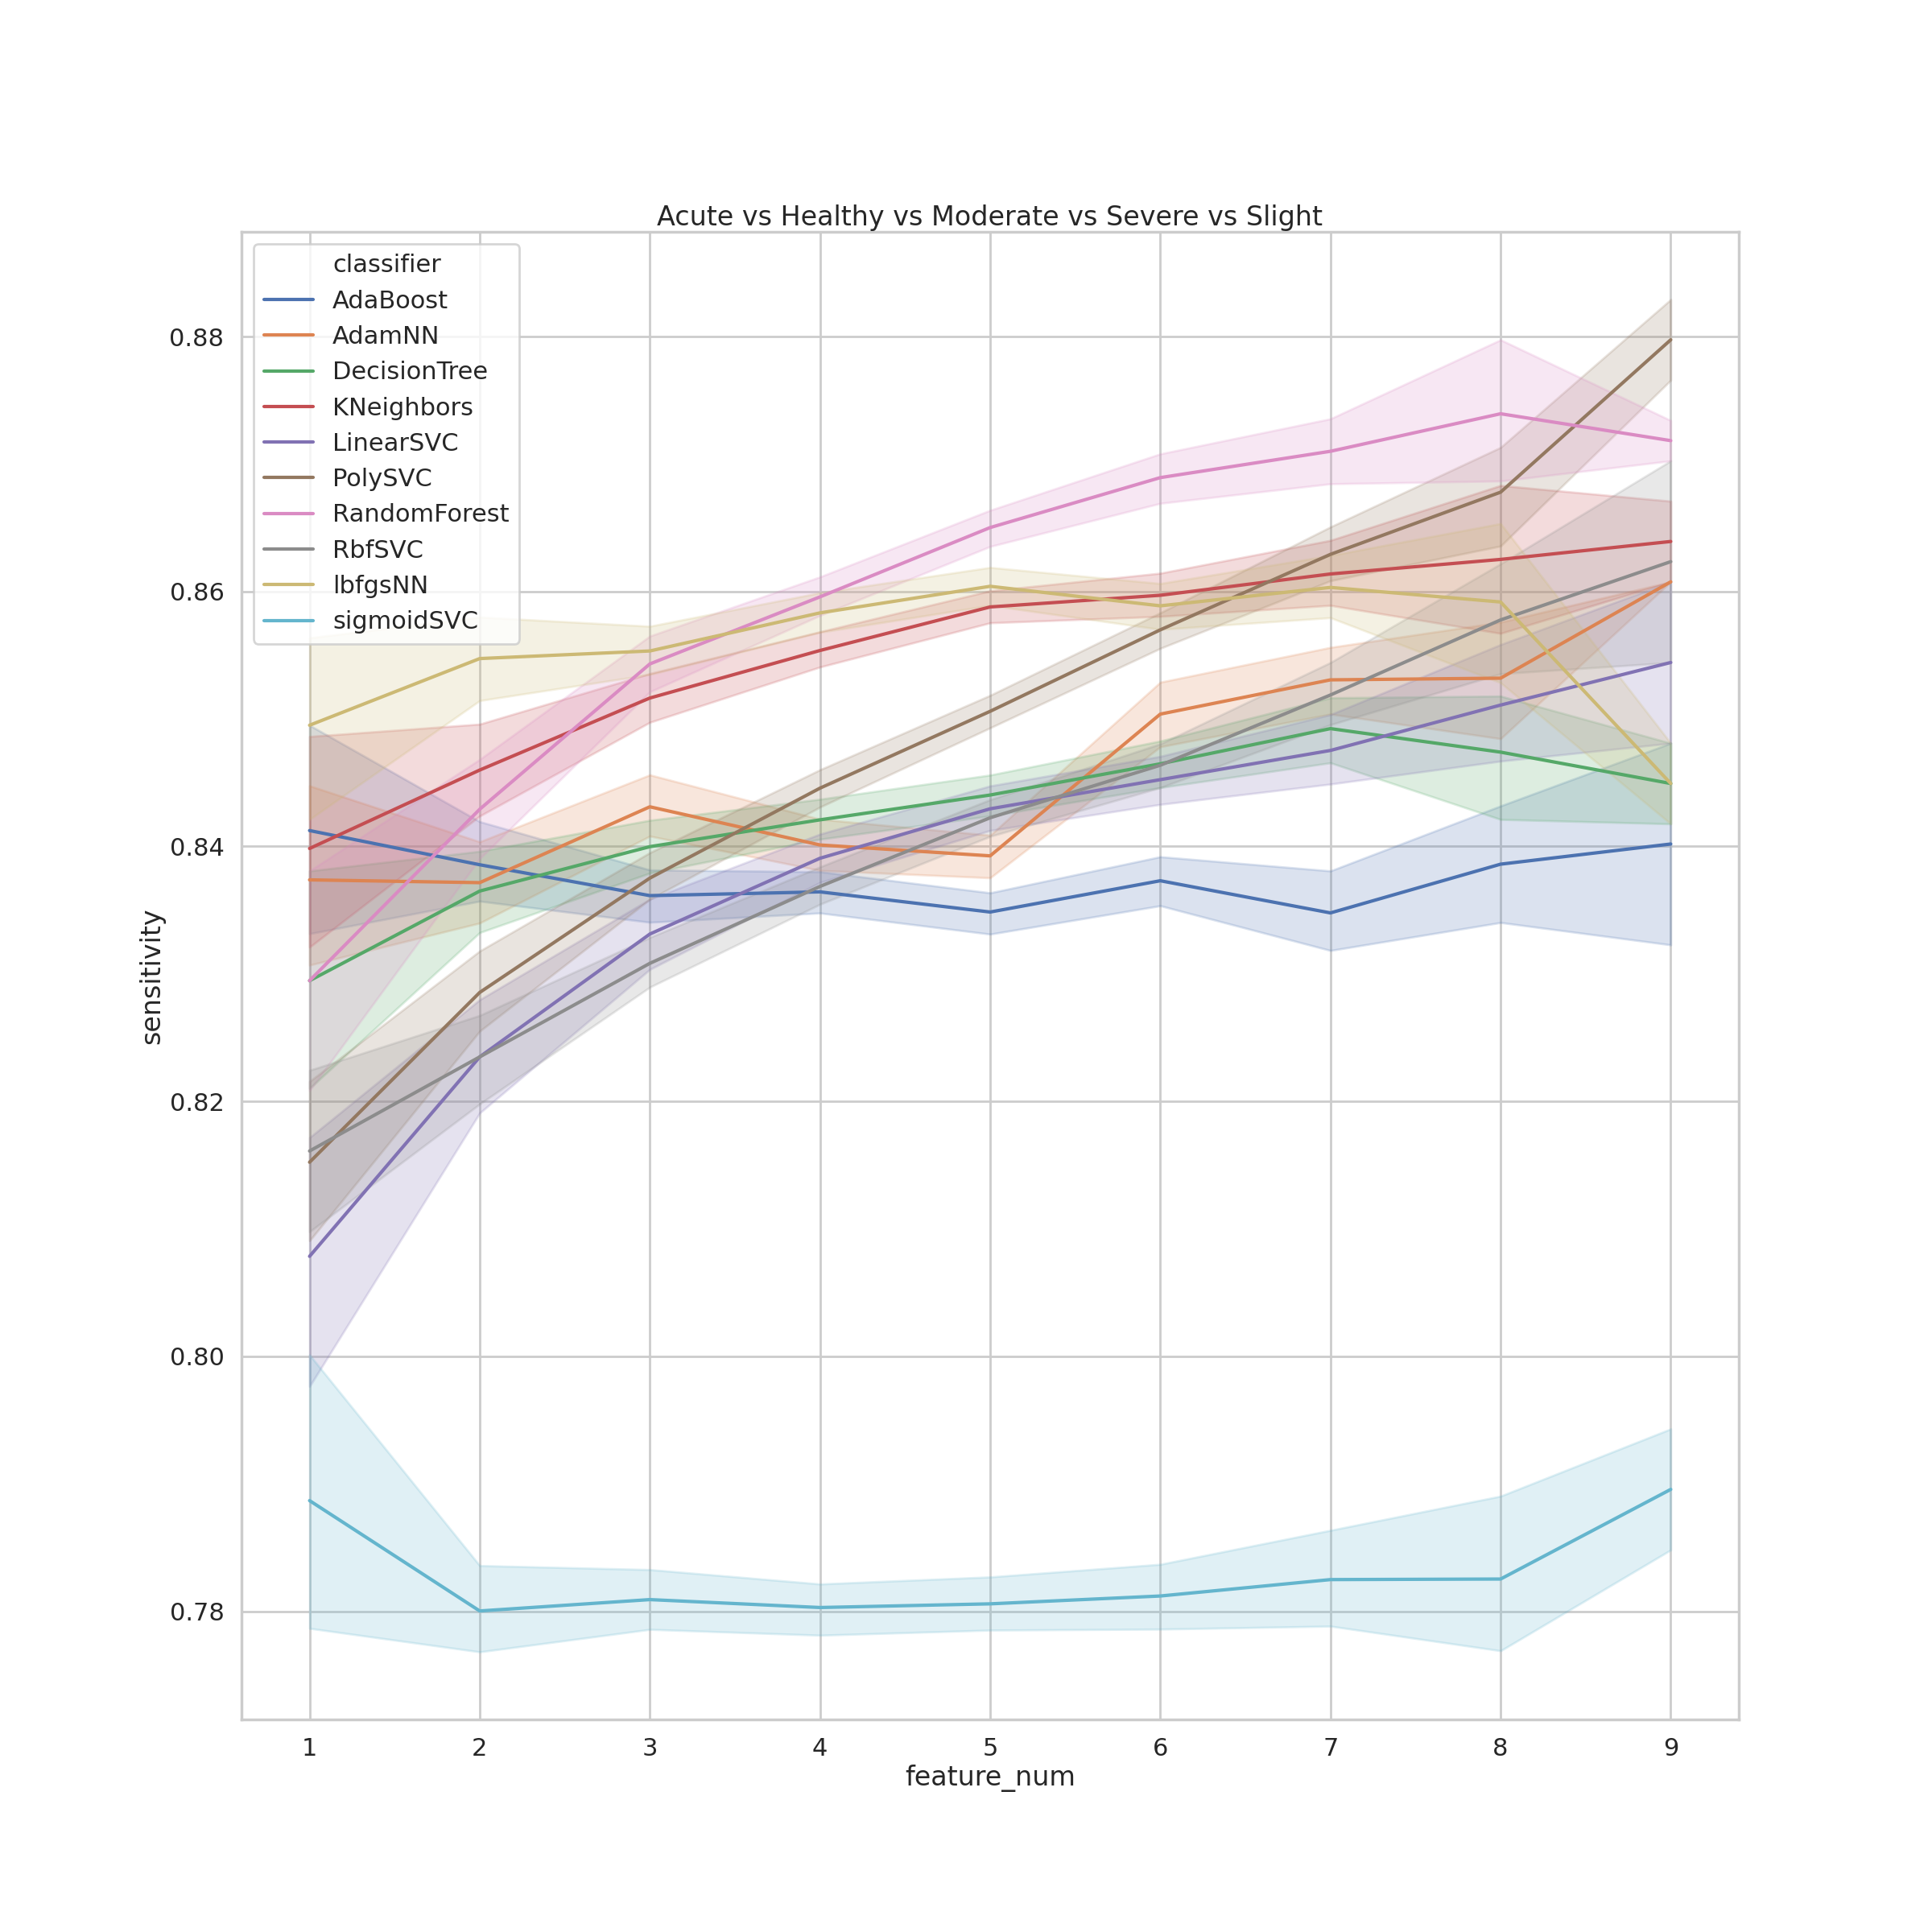
\includegraphics[width=0.3 \linewidth]{figures/5-class/sensitivity.png}
					&
					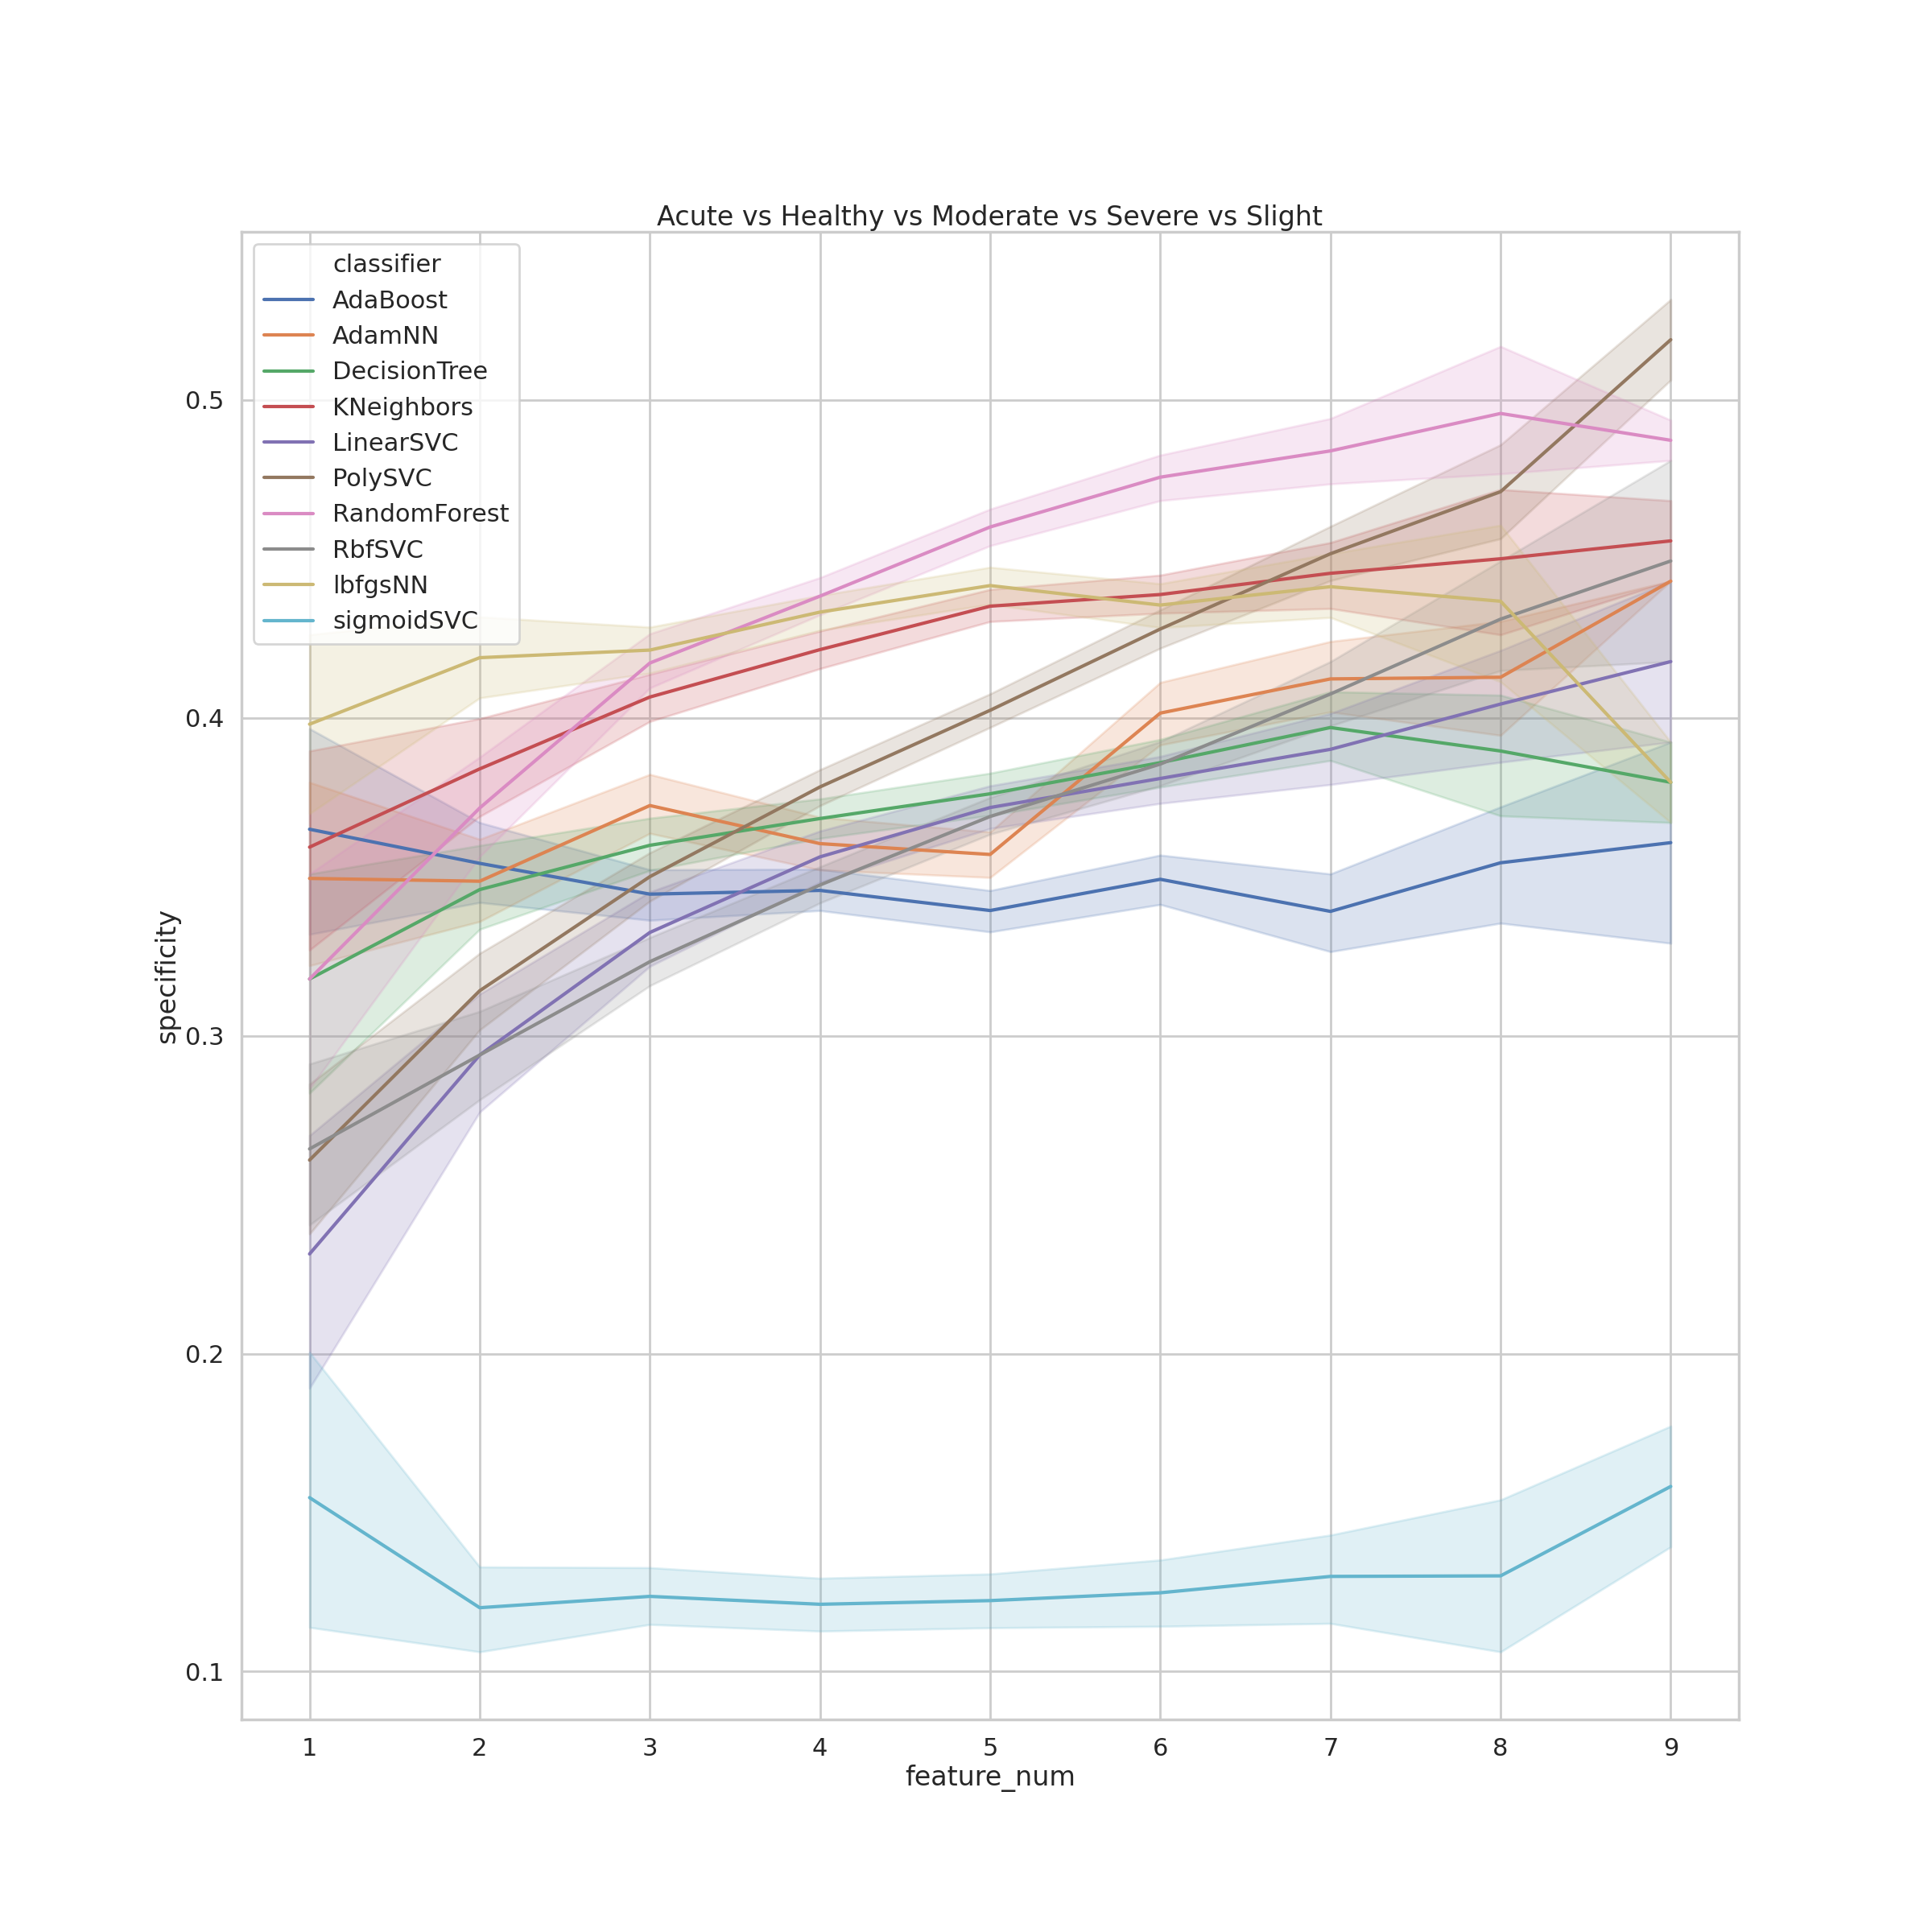
\includegraphics[width=0.3 \linewidth]{figures/5-class/specificity.png}
					&
					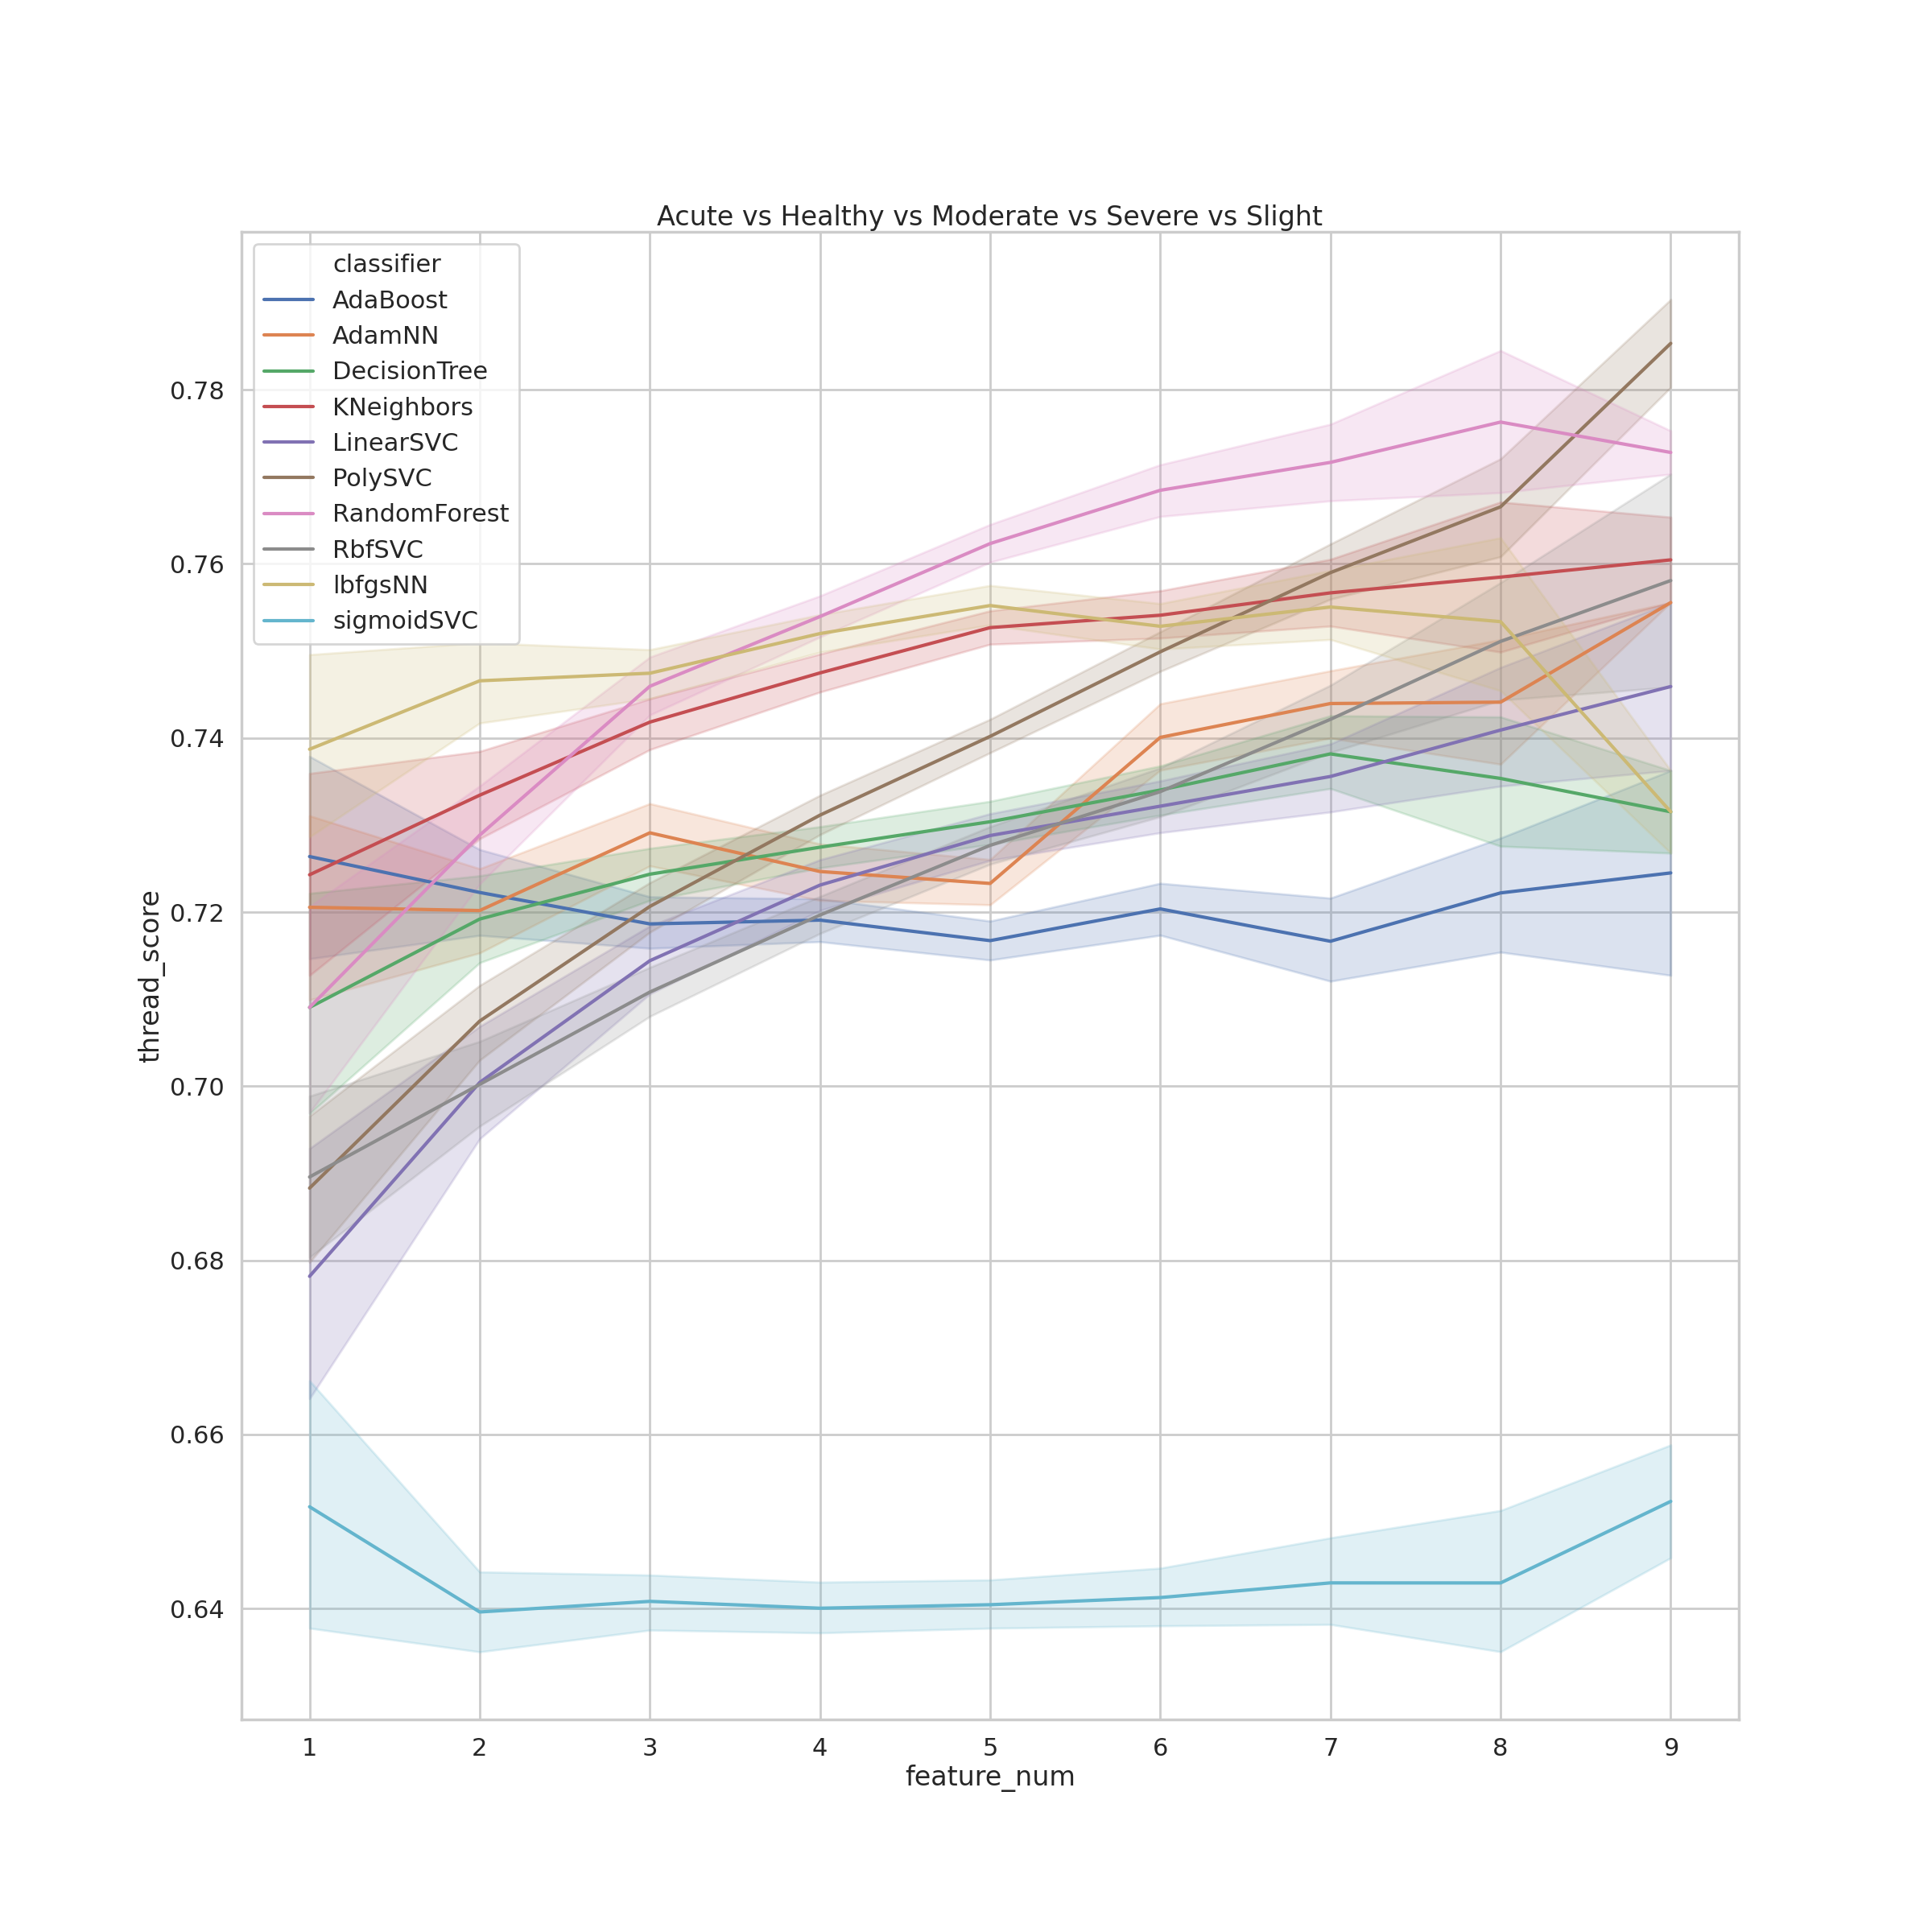
\includegraphics[width=0.3 \linewidth]{figures/5-class/thread_score.png}
					\\
					\mbox{Sensitivity} & \mbox{Specificity} & \mbox{Thread score} \\
				\end{array}$
				\caption{Confusion Matrix Derivations from 5-class Classification}
				\label{fig:5-confusion}
    		\end{figure}
    	
    		As figure \ref{fig:5-confusion}, the Poly-SVC algorithm has the best values with all features. 
    		
    		\begin{figure}[htbp]
				\centering
				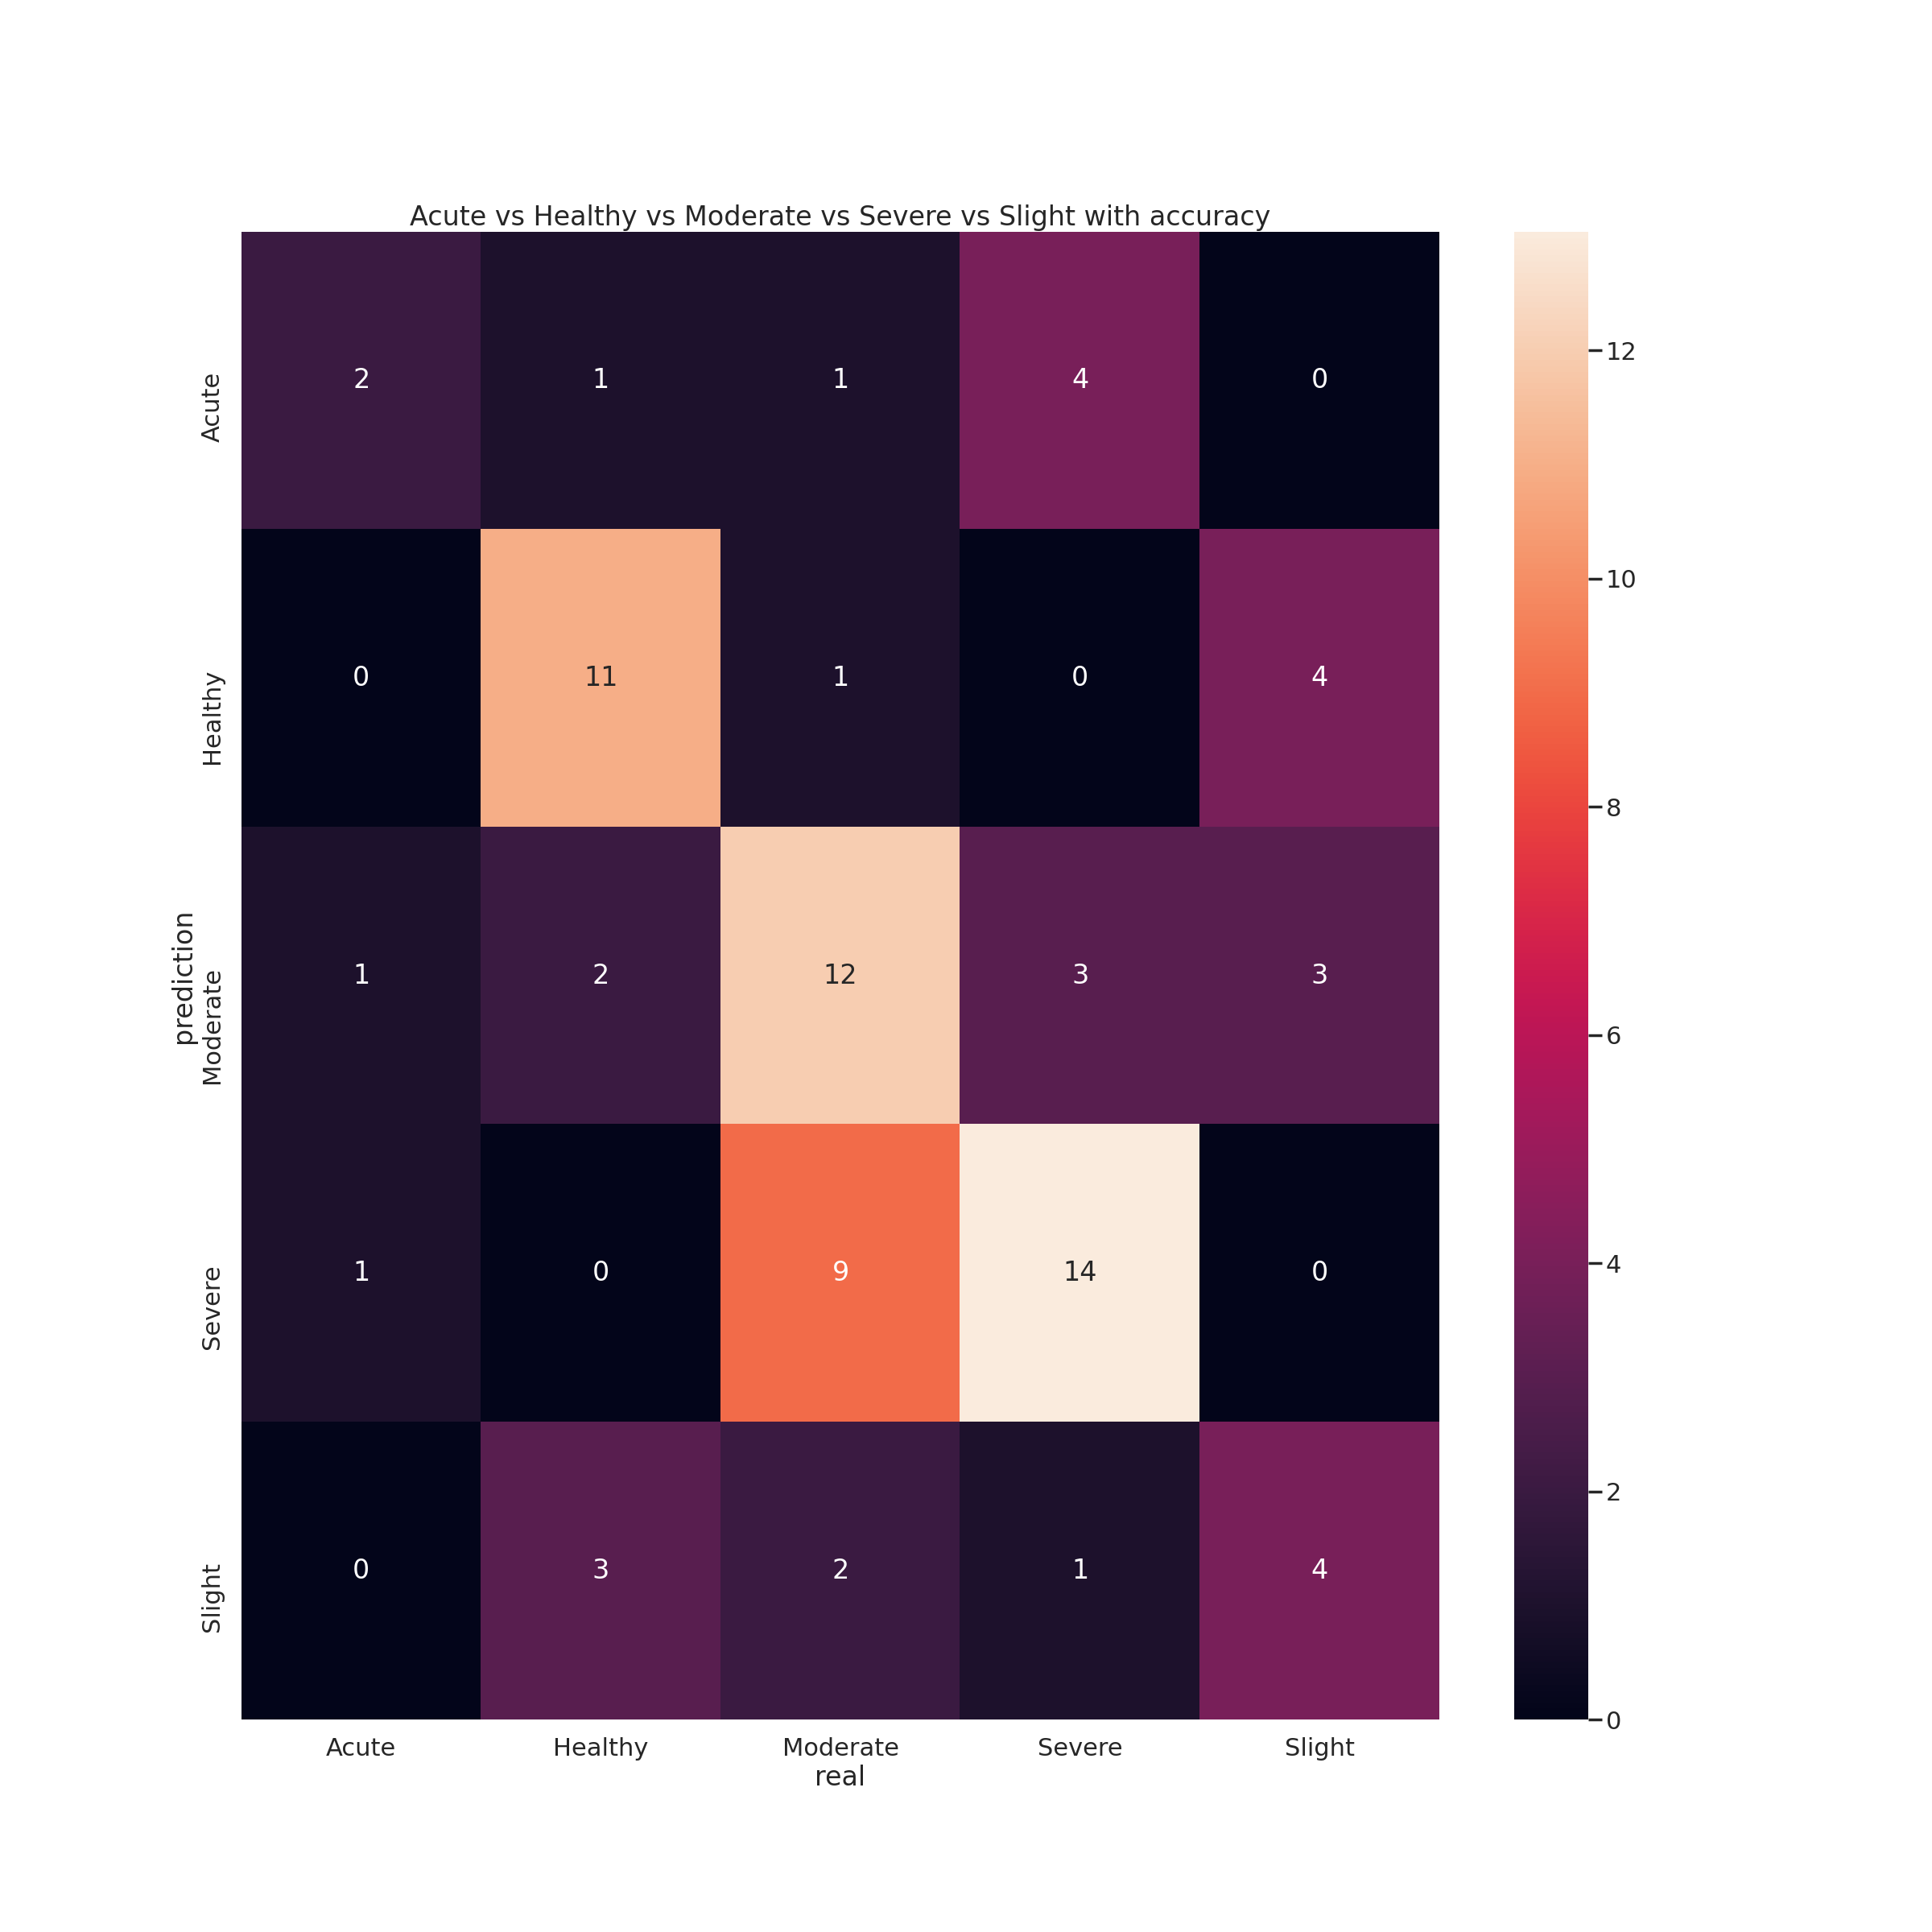
\includegraphics[width=0.5 \linewidth]{figures/5-class/heatmap.png}
				\caption{Heatmap Plot for 5-class Classification with Poly-SVC}
				\label{fig:5-heatmap}
    		\end{figure}
    	
    		Figure \ref{fig:5-heatmap} shows the heatmap between real and predicted classes. As shown as figure \ref{fig:5-confusion}, the accuracy is over 80 \%, and wrong predicted class is predicted neighbor class; for instance, healthy and moderate class are neighbor class of slight class. Moreover, acute class is commonly classified as moderate and severe class. 
    		
    	\subsection{4-class Classification}
    		\subsubsection{Merged Healthy-Slight Class}
    			Figure \ref{fig:h-sli-confusion} displays the derivations of confusion matrix in merged healthy-slight classification. Note that the values in figure \ref{fig:h-sli-confusion}, mean values from combination which used same number of features will be shown. As figure \ref{fig:h-sli-confusion}, the Random Forest algorithm has the best values with all features. 
    			
	    		\begin{figure}[htbp]
    				\centering
	    				$\begin{array}{ccc}
	    				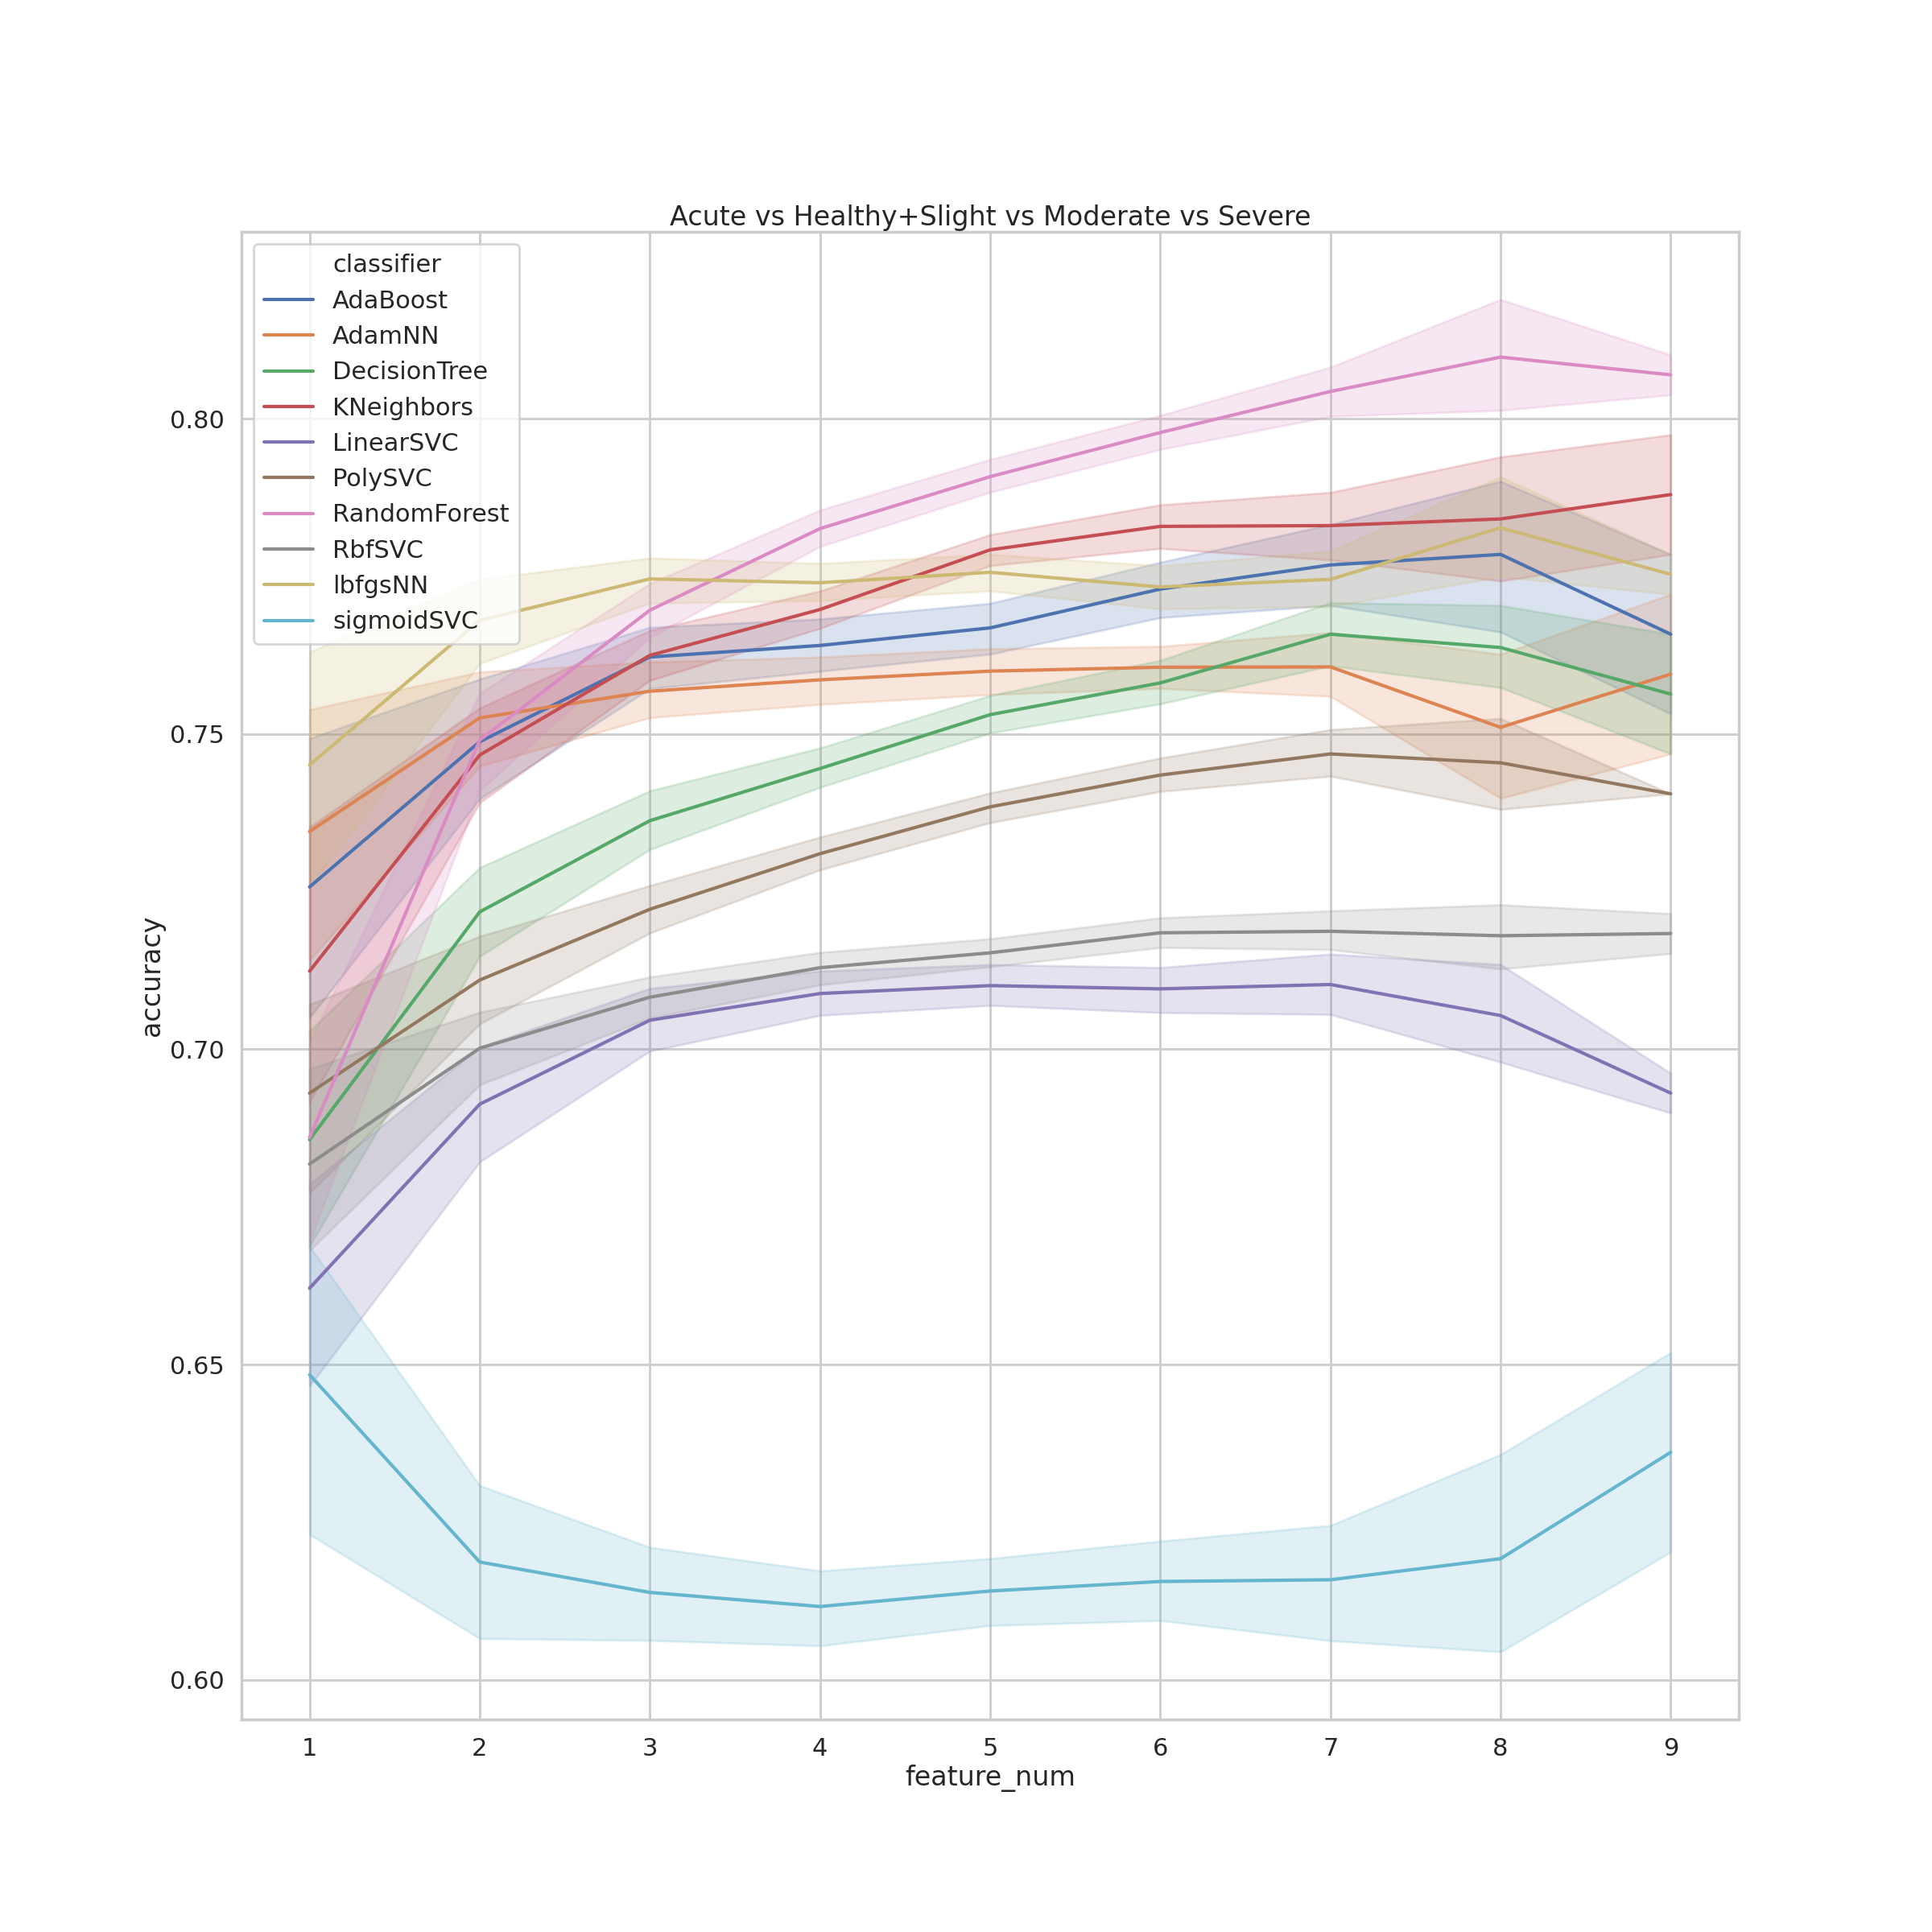
\includegraphics[width=0.3 \linewidth]{figures/Healthy-Slight/accuracy.png}
	    				&
	    				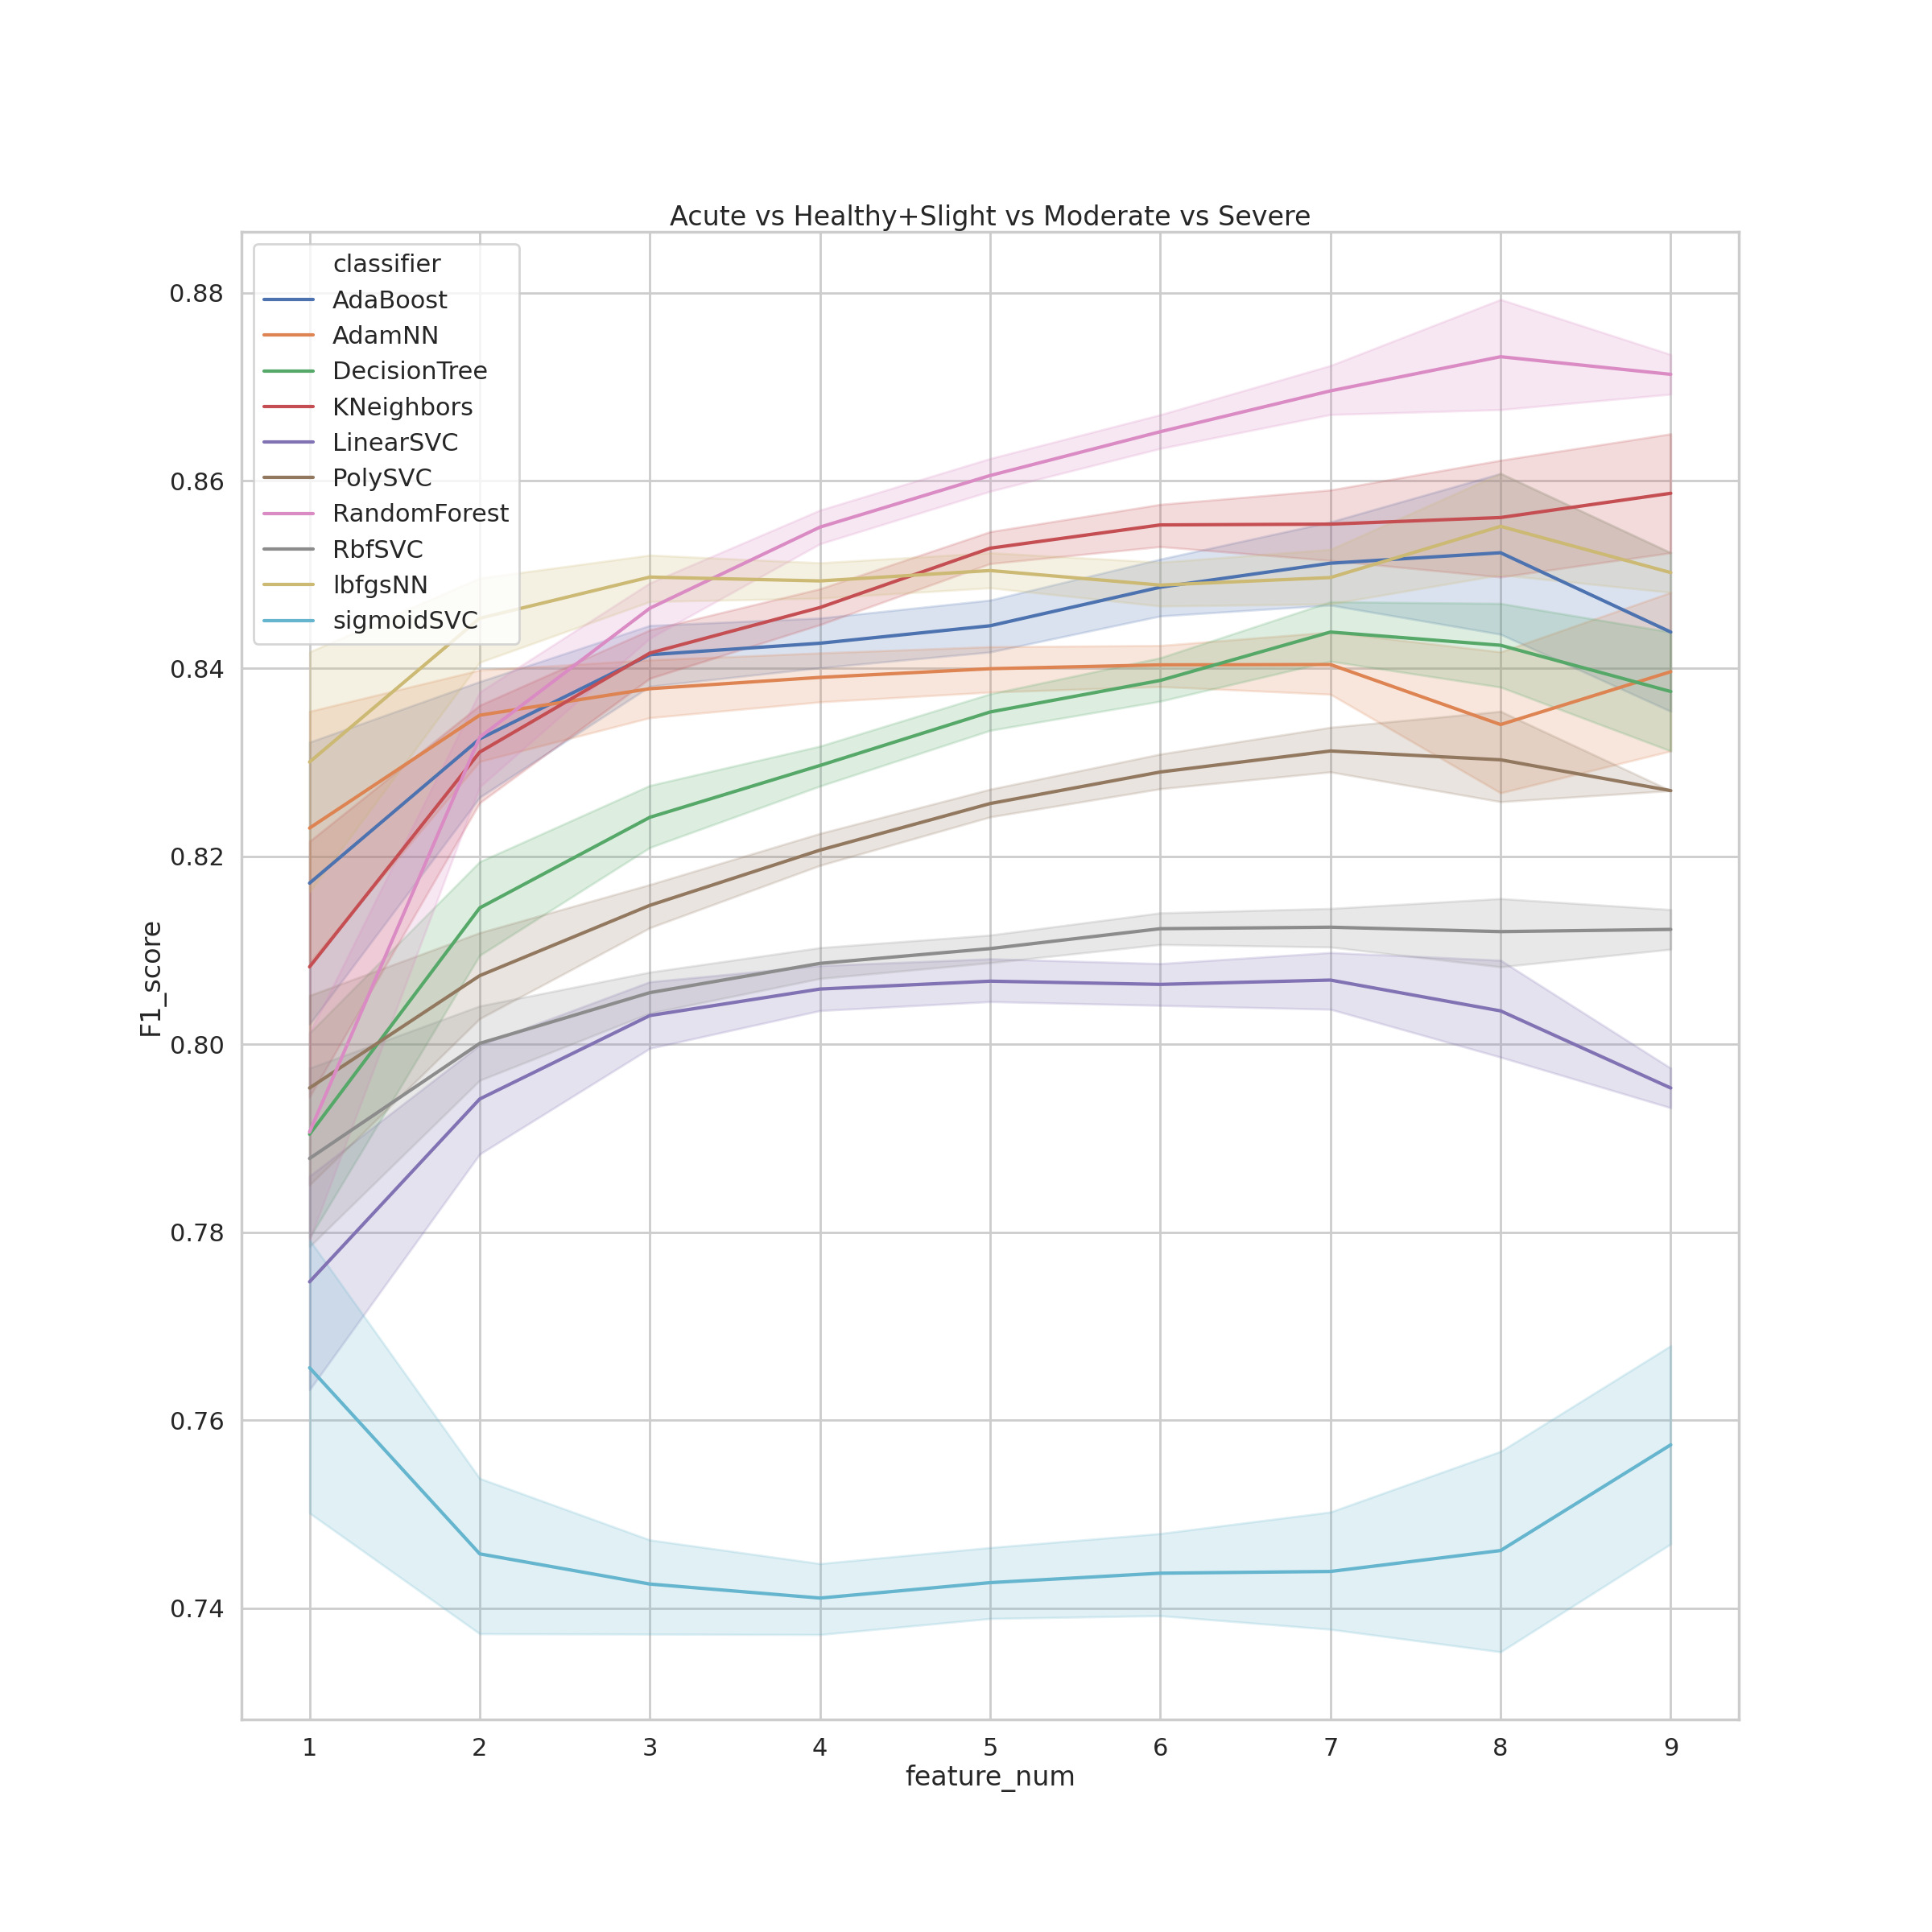
\includegraphics[width=0.3 \linewidth]{figures/Healthy-Slight/F1_score.png}
	    				&
	    				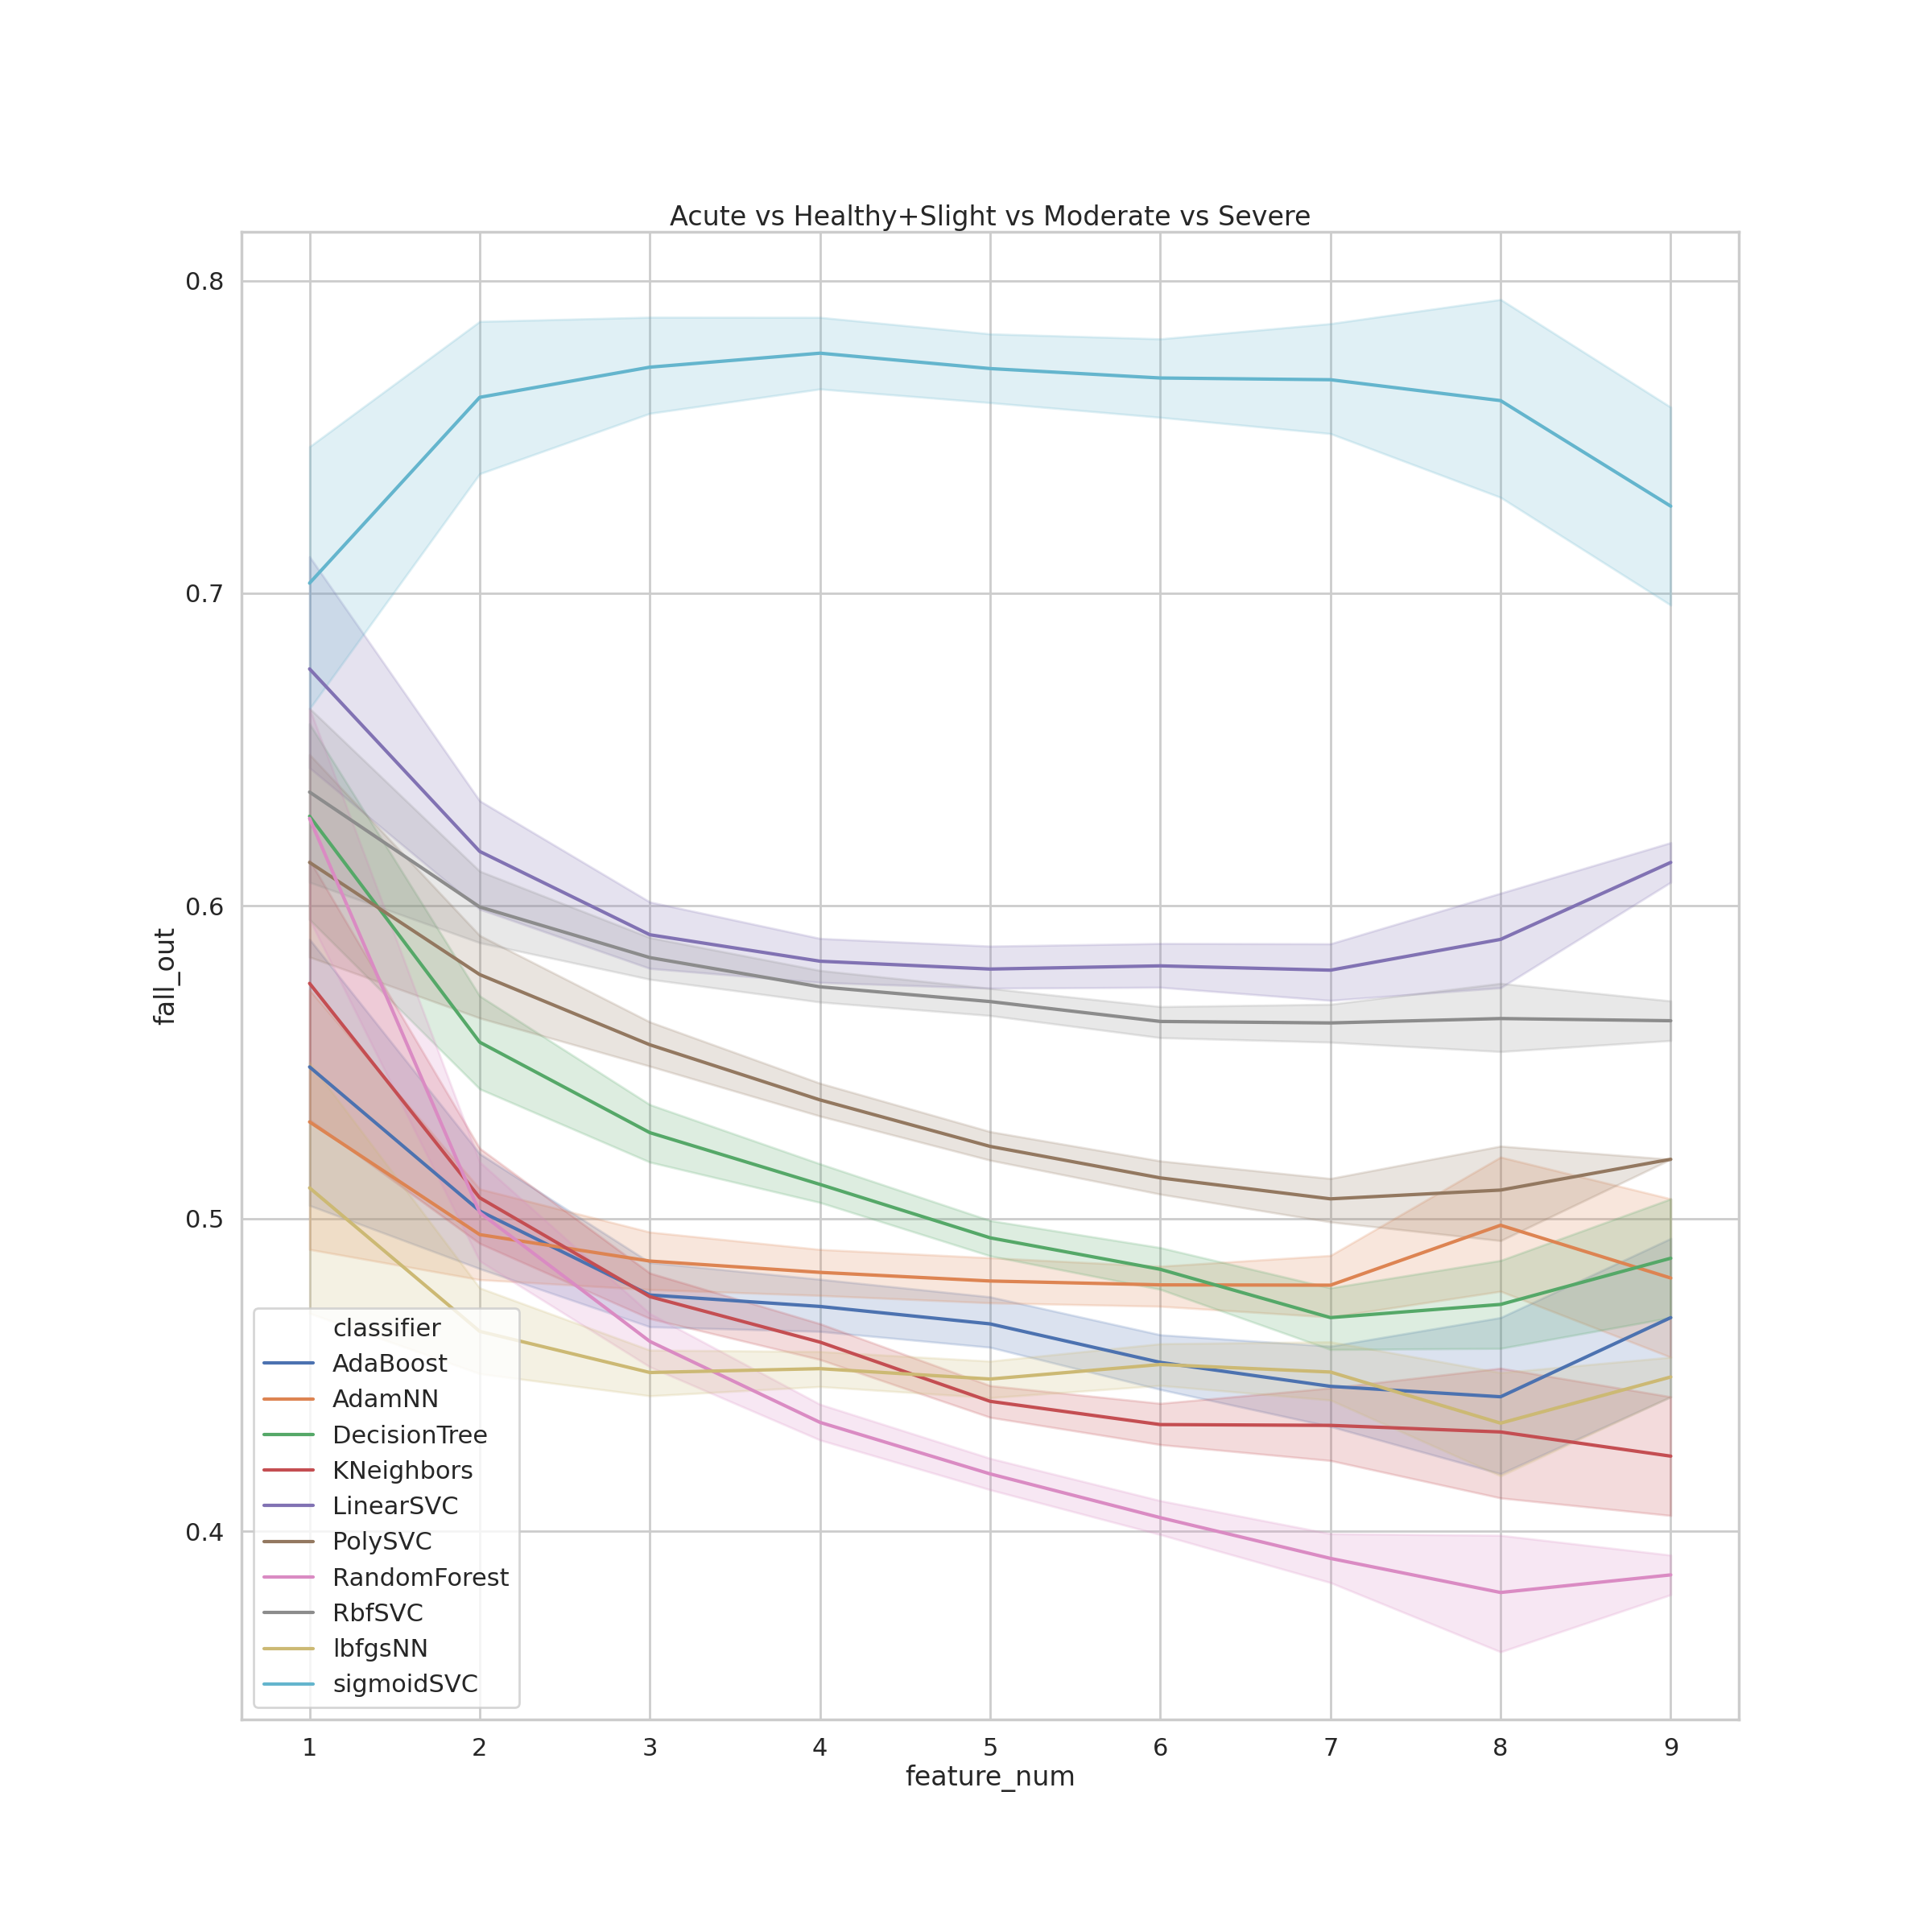
\includegraphics[width=0.3 \linewidth]{figures/Healthy-Slight/fall_out.png}
	    				\\
	    				\mbox{Accuracy} & \mbox{F1 score} & \mbox{Fall-out} \\
	    				
	    				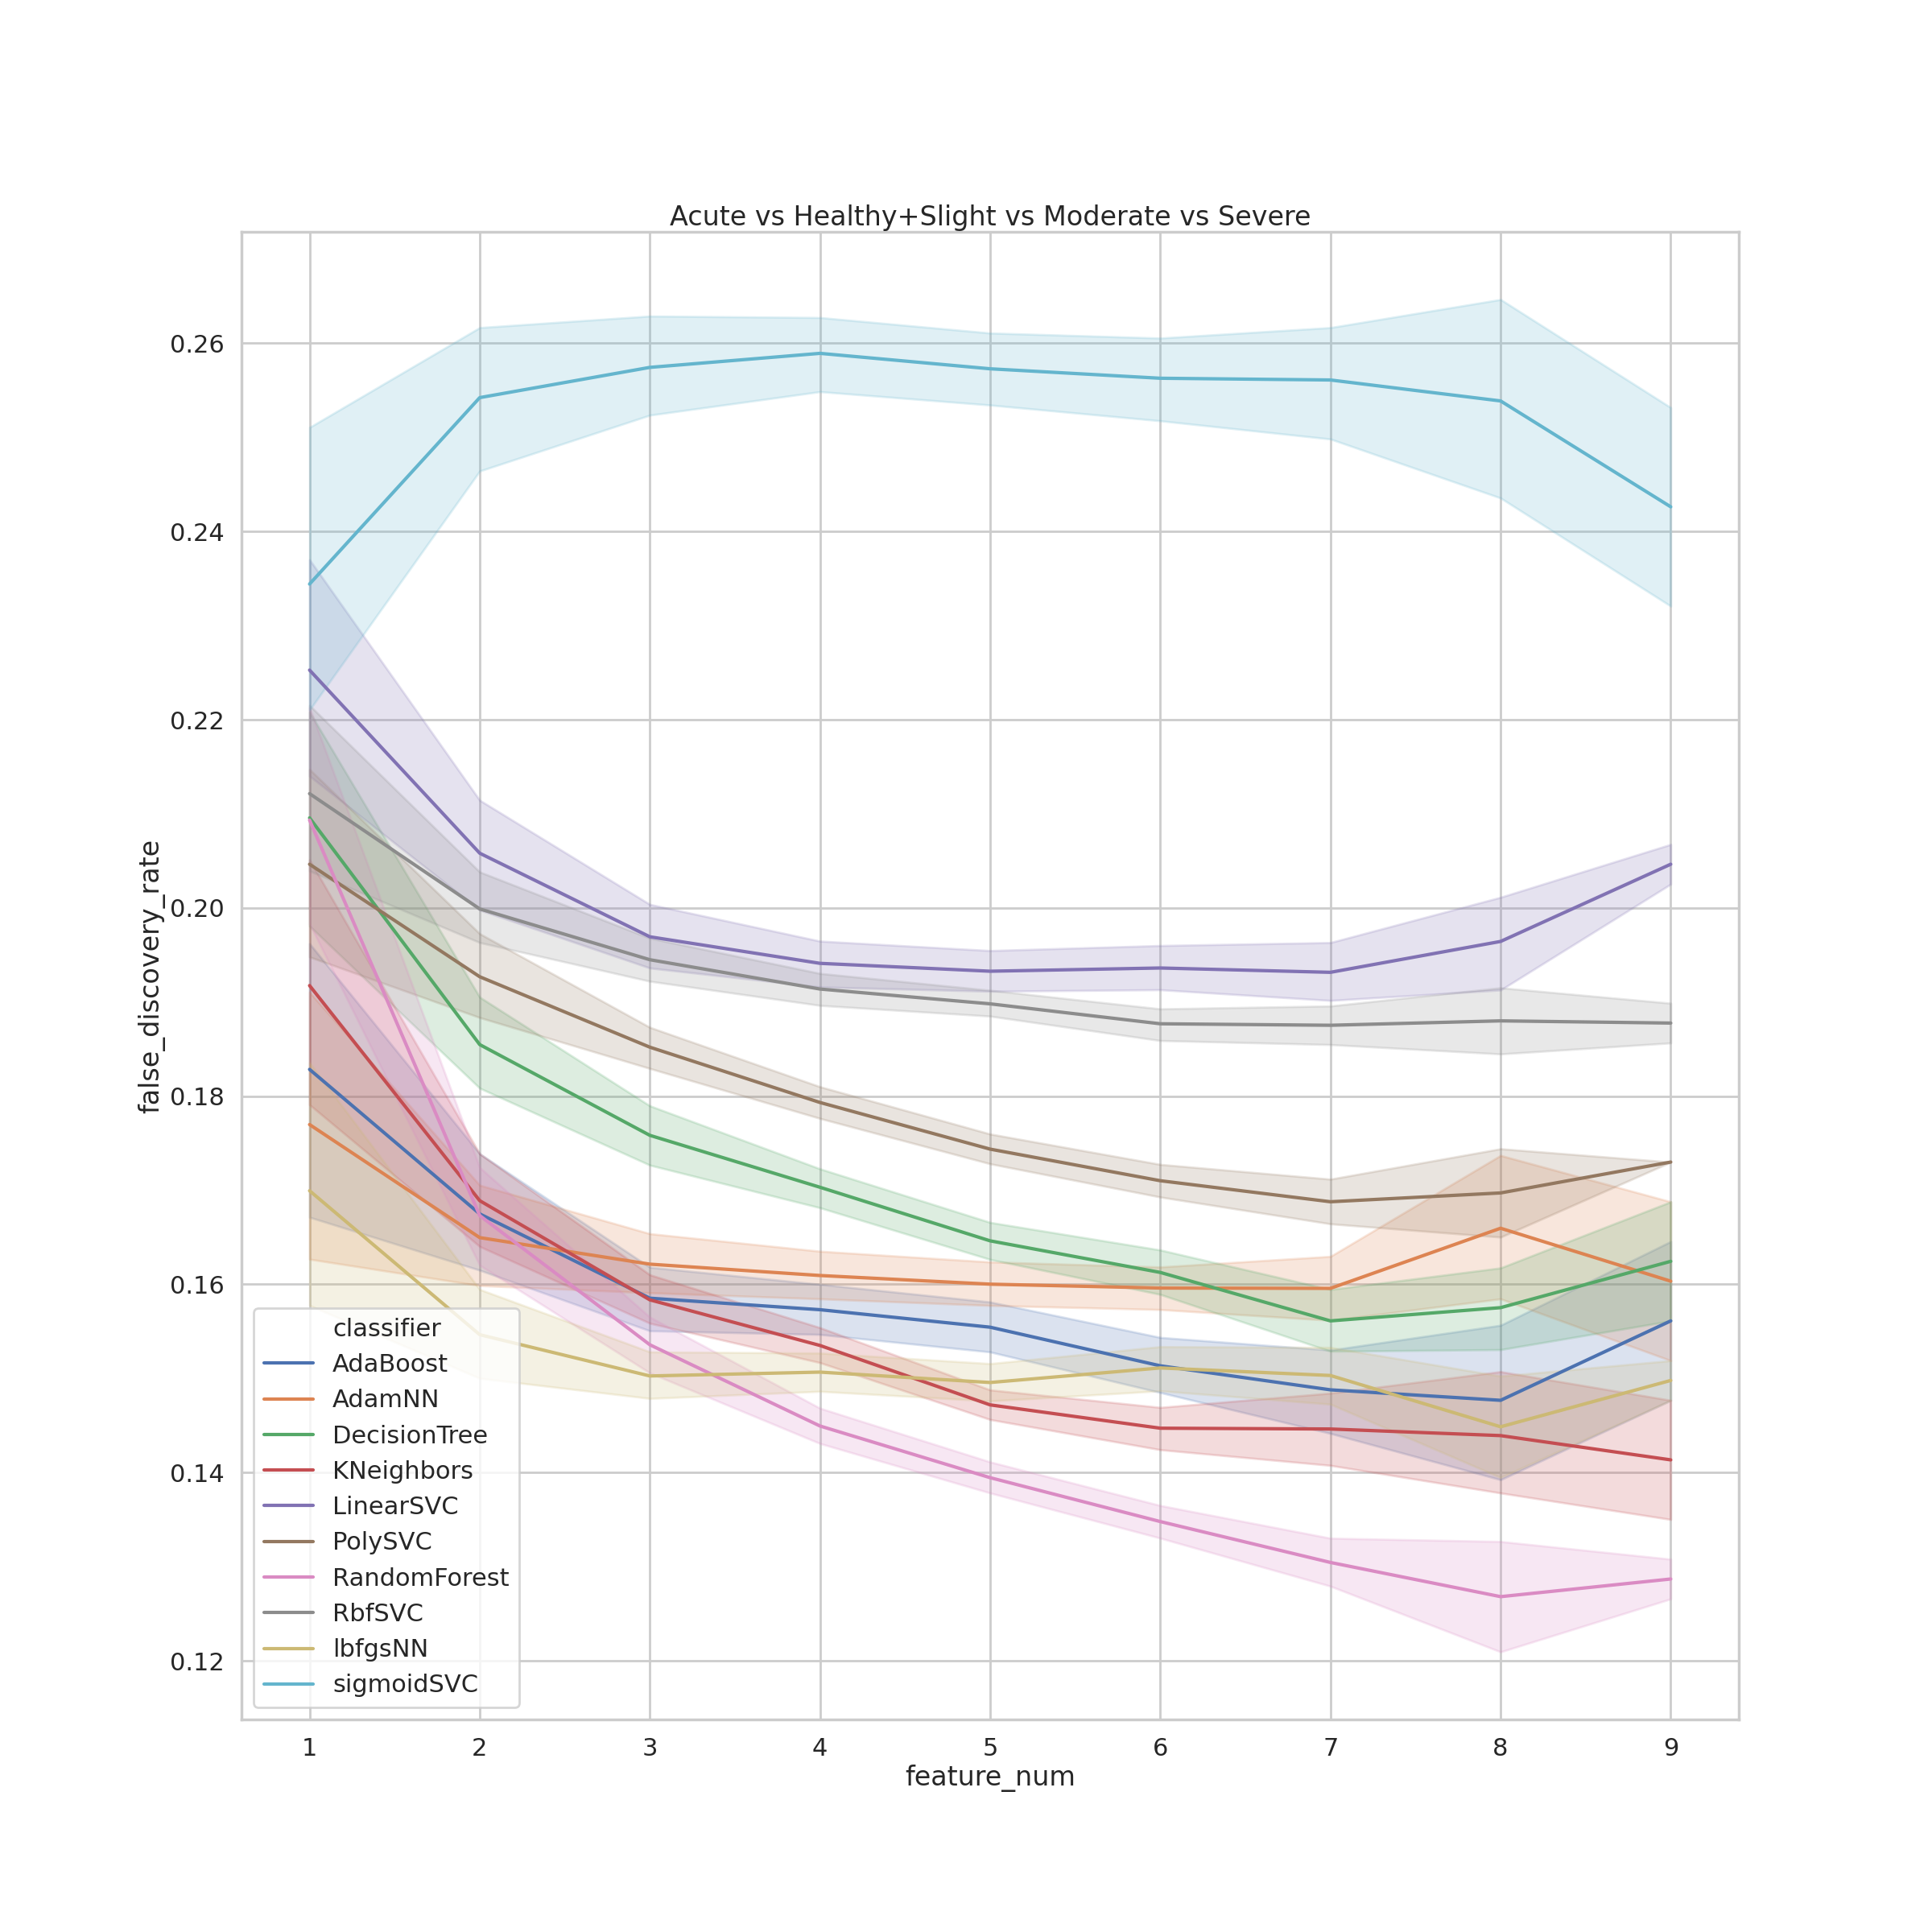
\includegraphics[width=0.3 \linewidth]{figures/Healthy-Slight/false_discovery_rate.png}
	    				&
	    				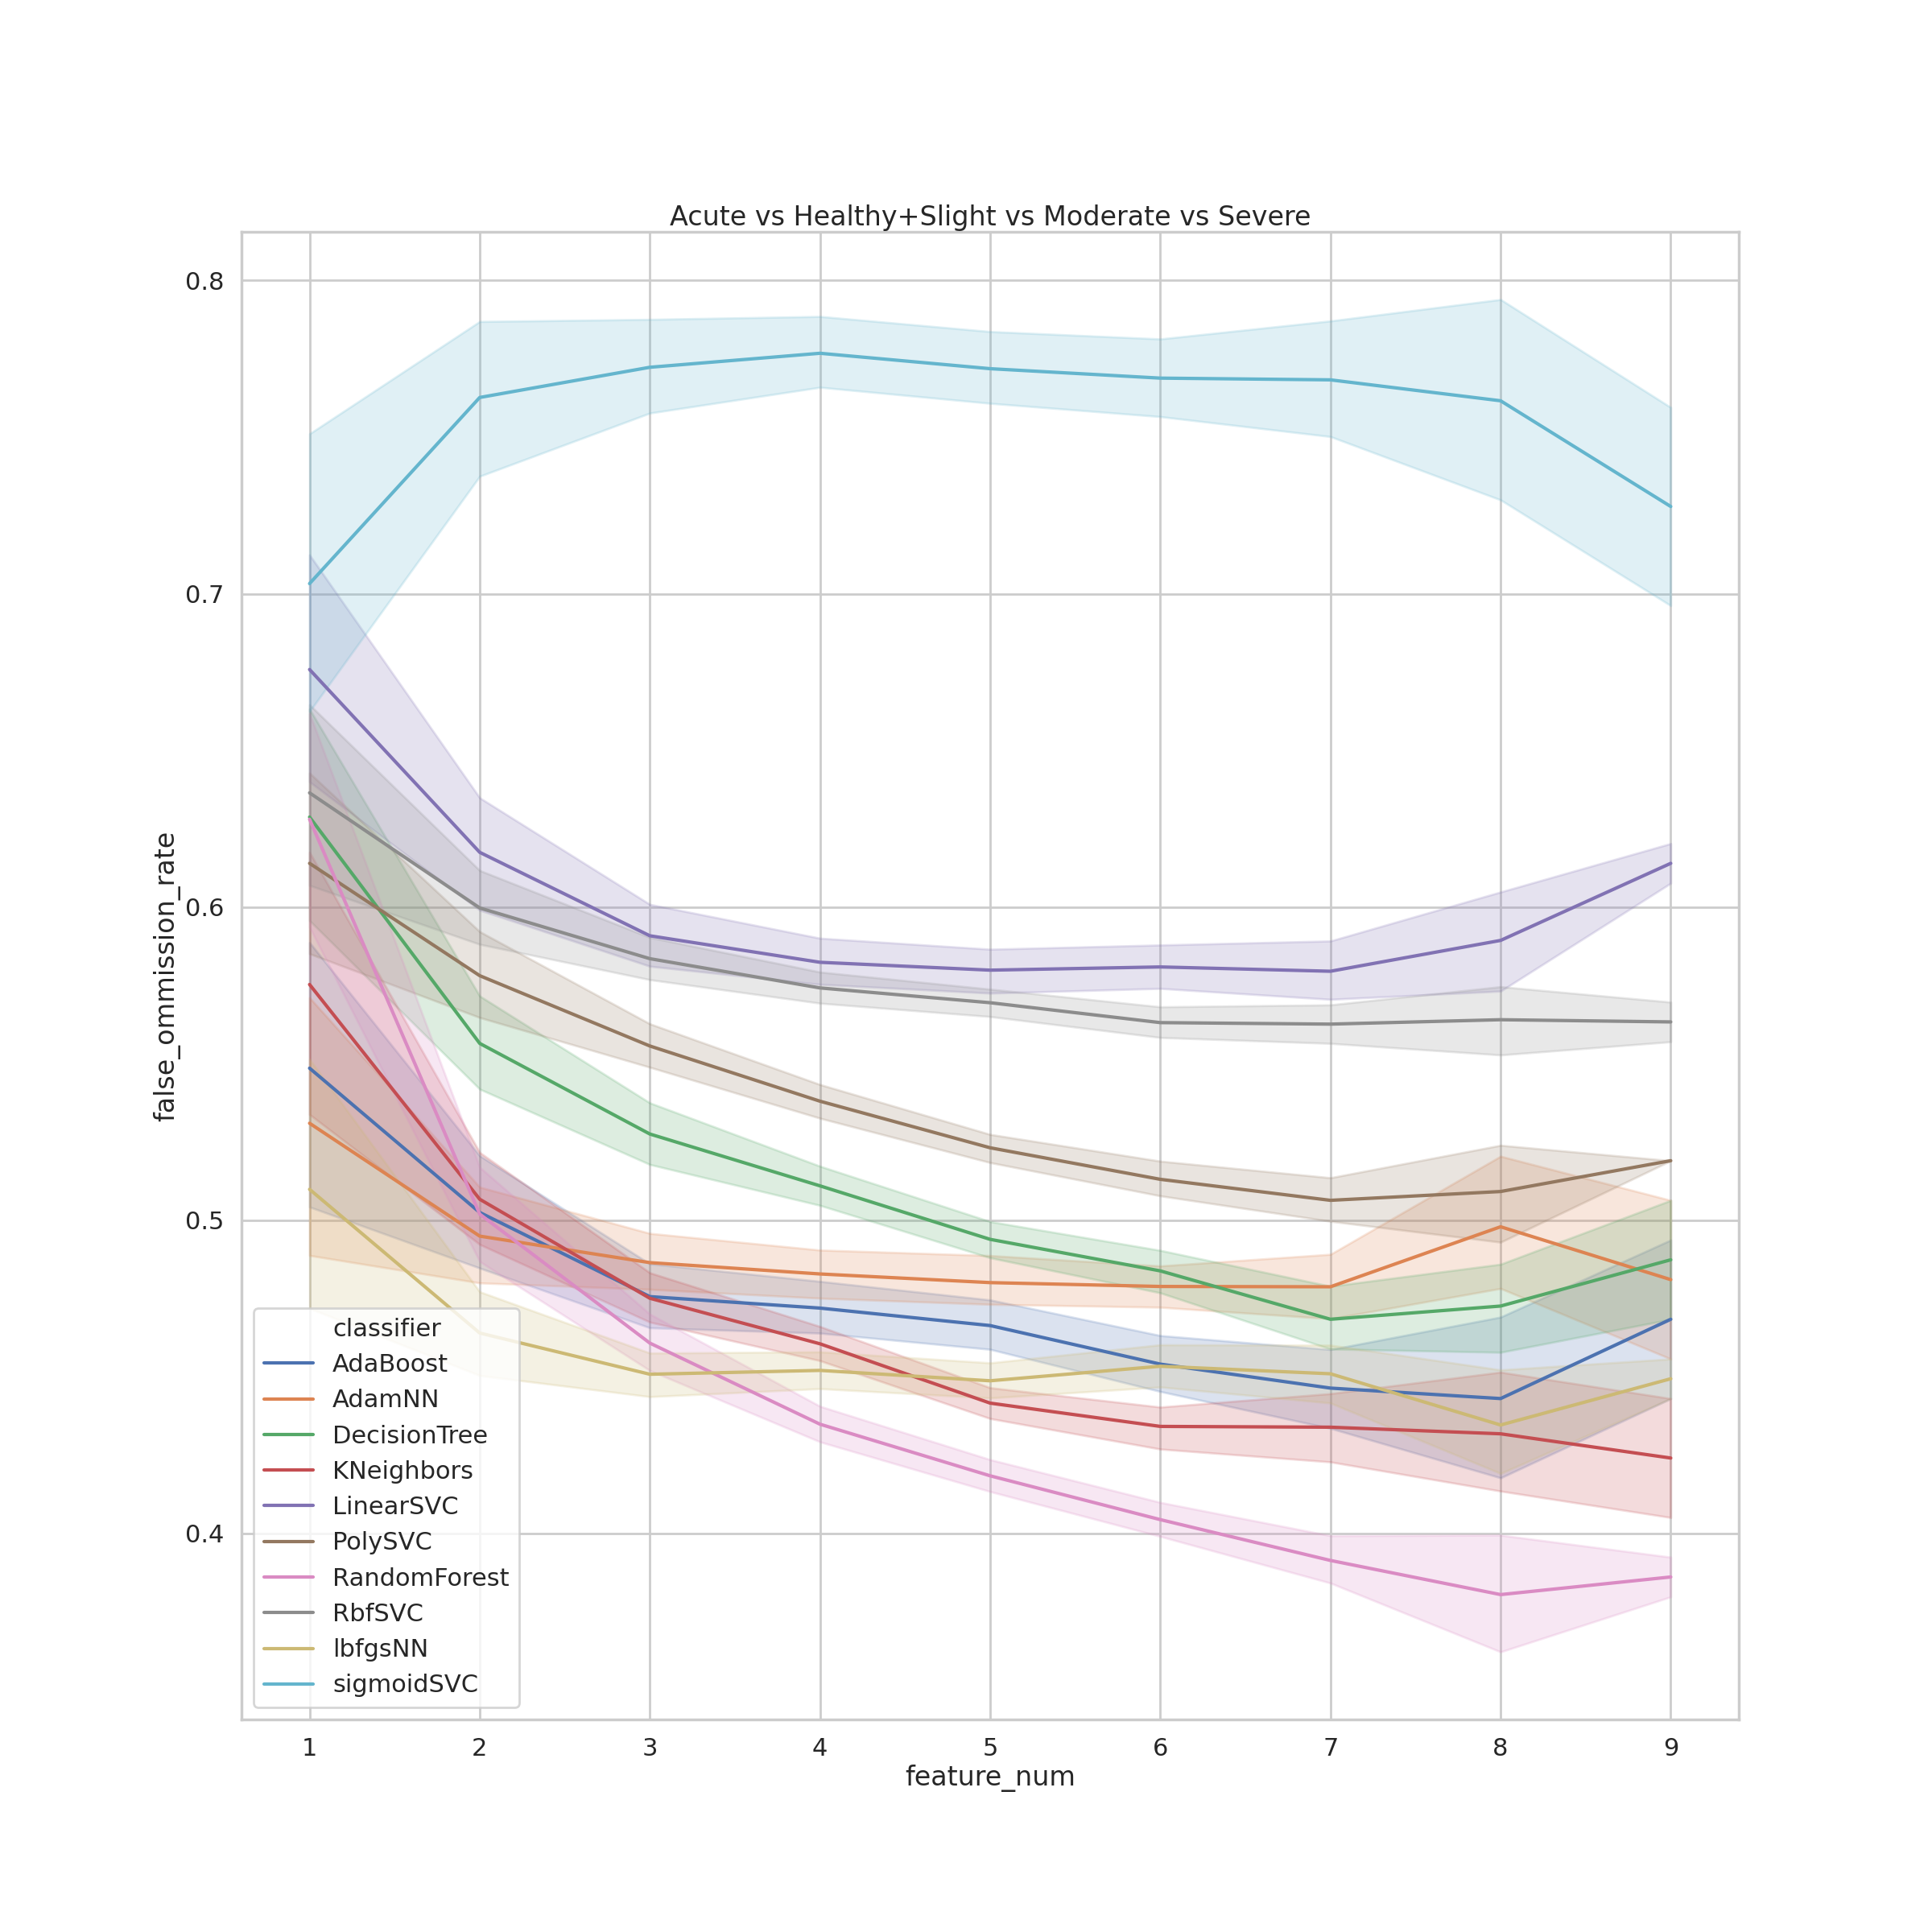
\includegraphics[width=0.3 \linewidth]{figures/Healthy-Slight/false_ommission_rate.png}
	    				&
	    				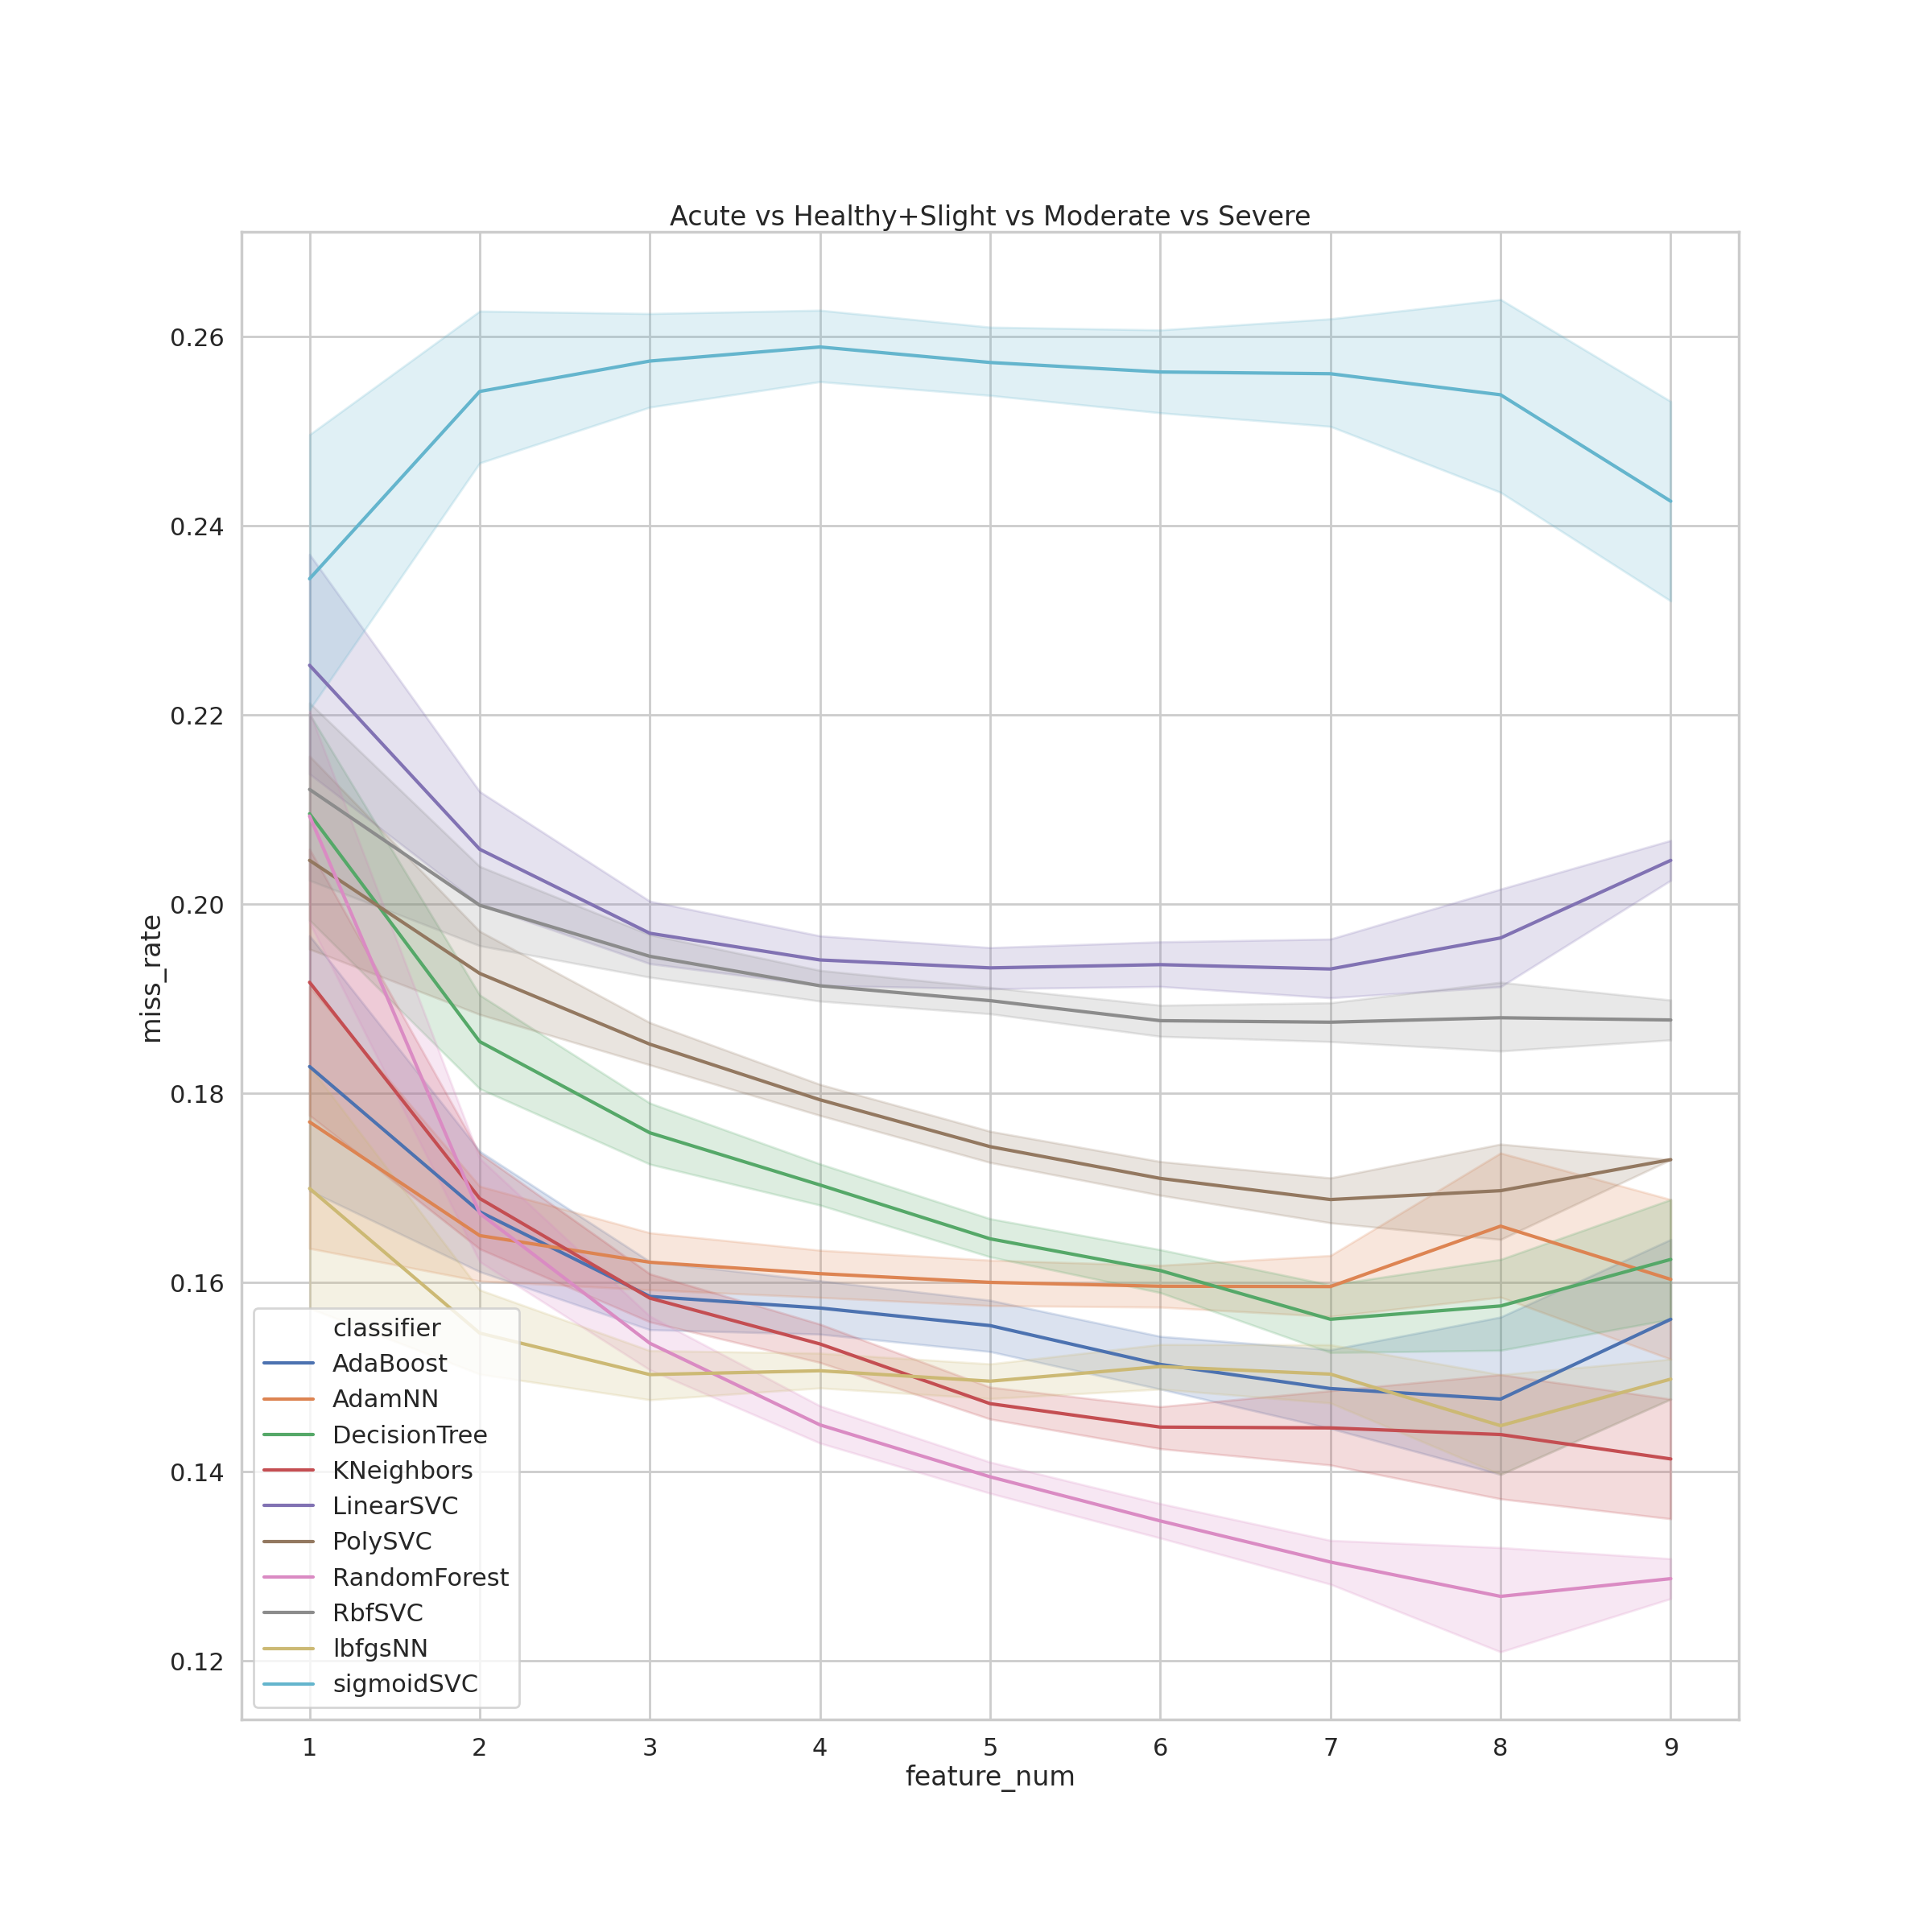
\includegraphics[width=0.3 \linewidth]{figures/Healthy-Slight/miss_rate.png}
	    				\\
	    				\mbox{False discovery rate} & \mbox{False ommision rate} & \mbox{Miss rate} \\ 
	    				
	    				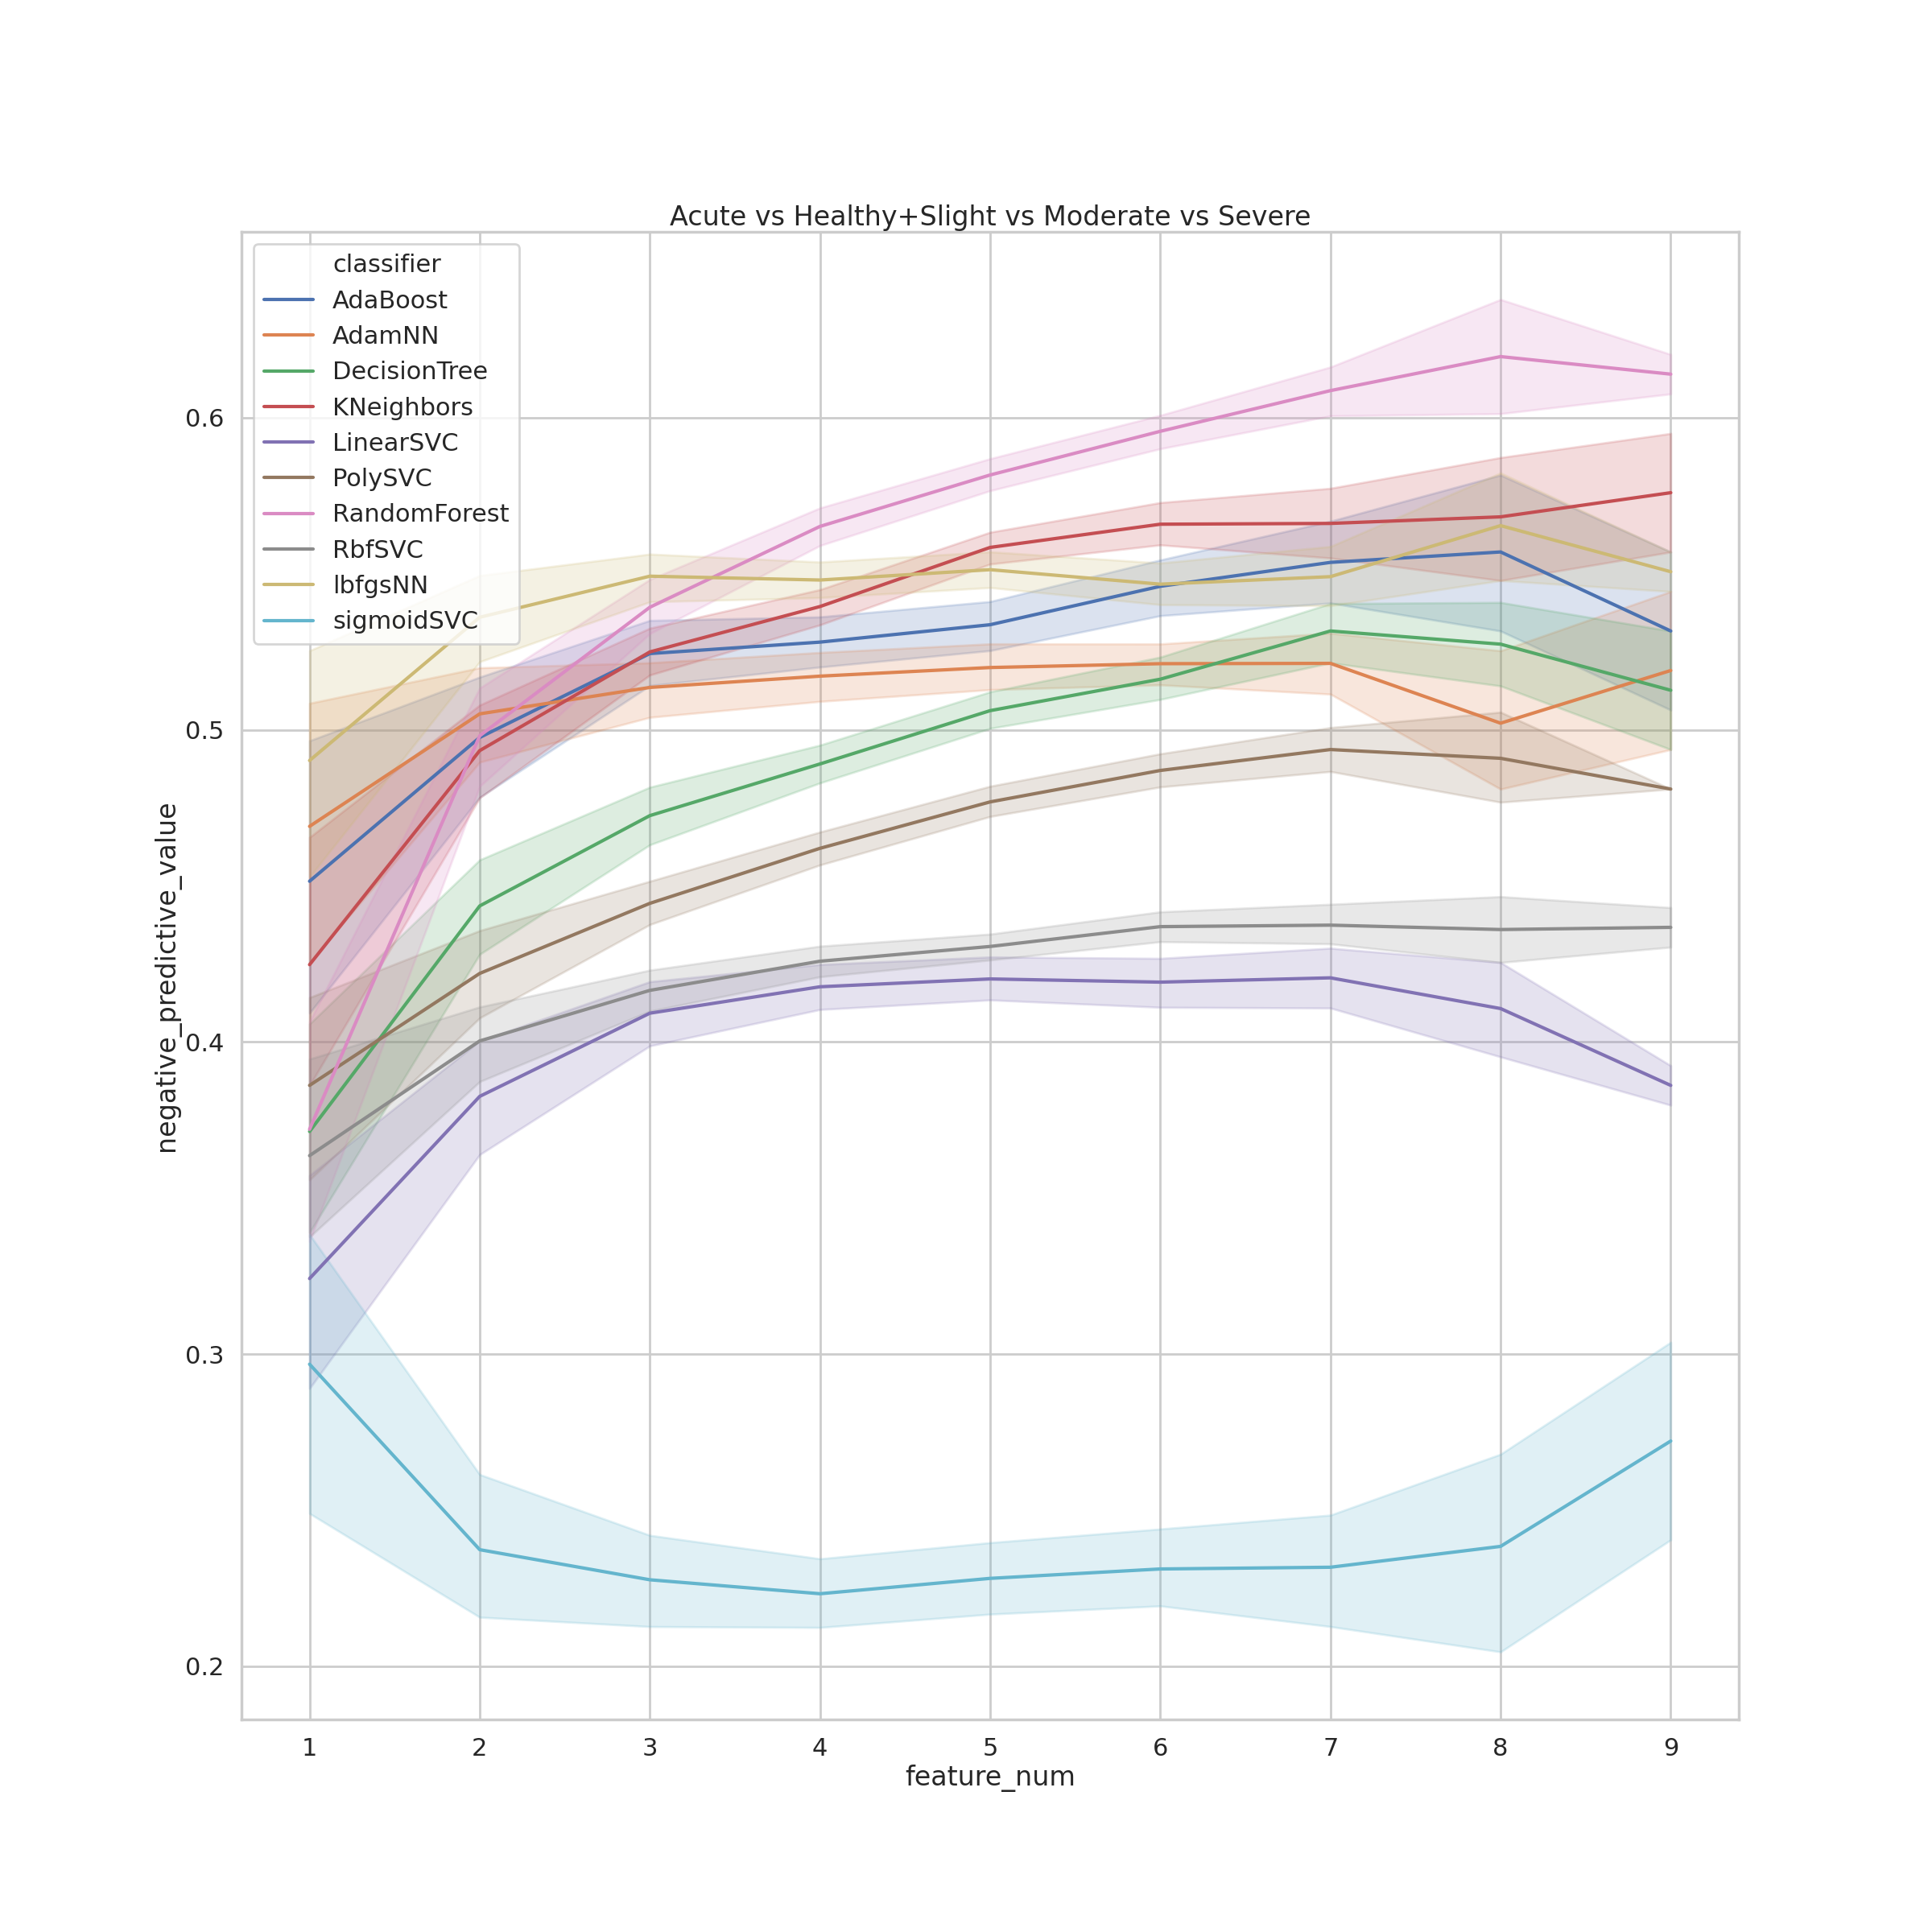
\includegraphics[width=0.3 \linewidth]{figures/Healthy-Slight/negative_predictive_value.png}
	    				&
	    				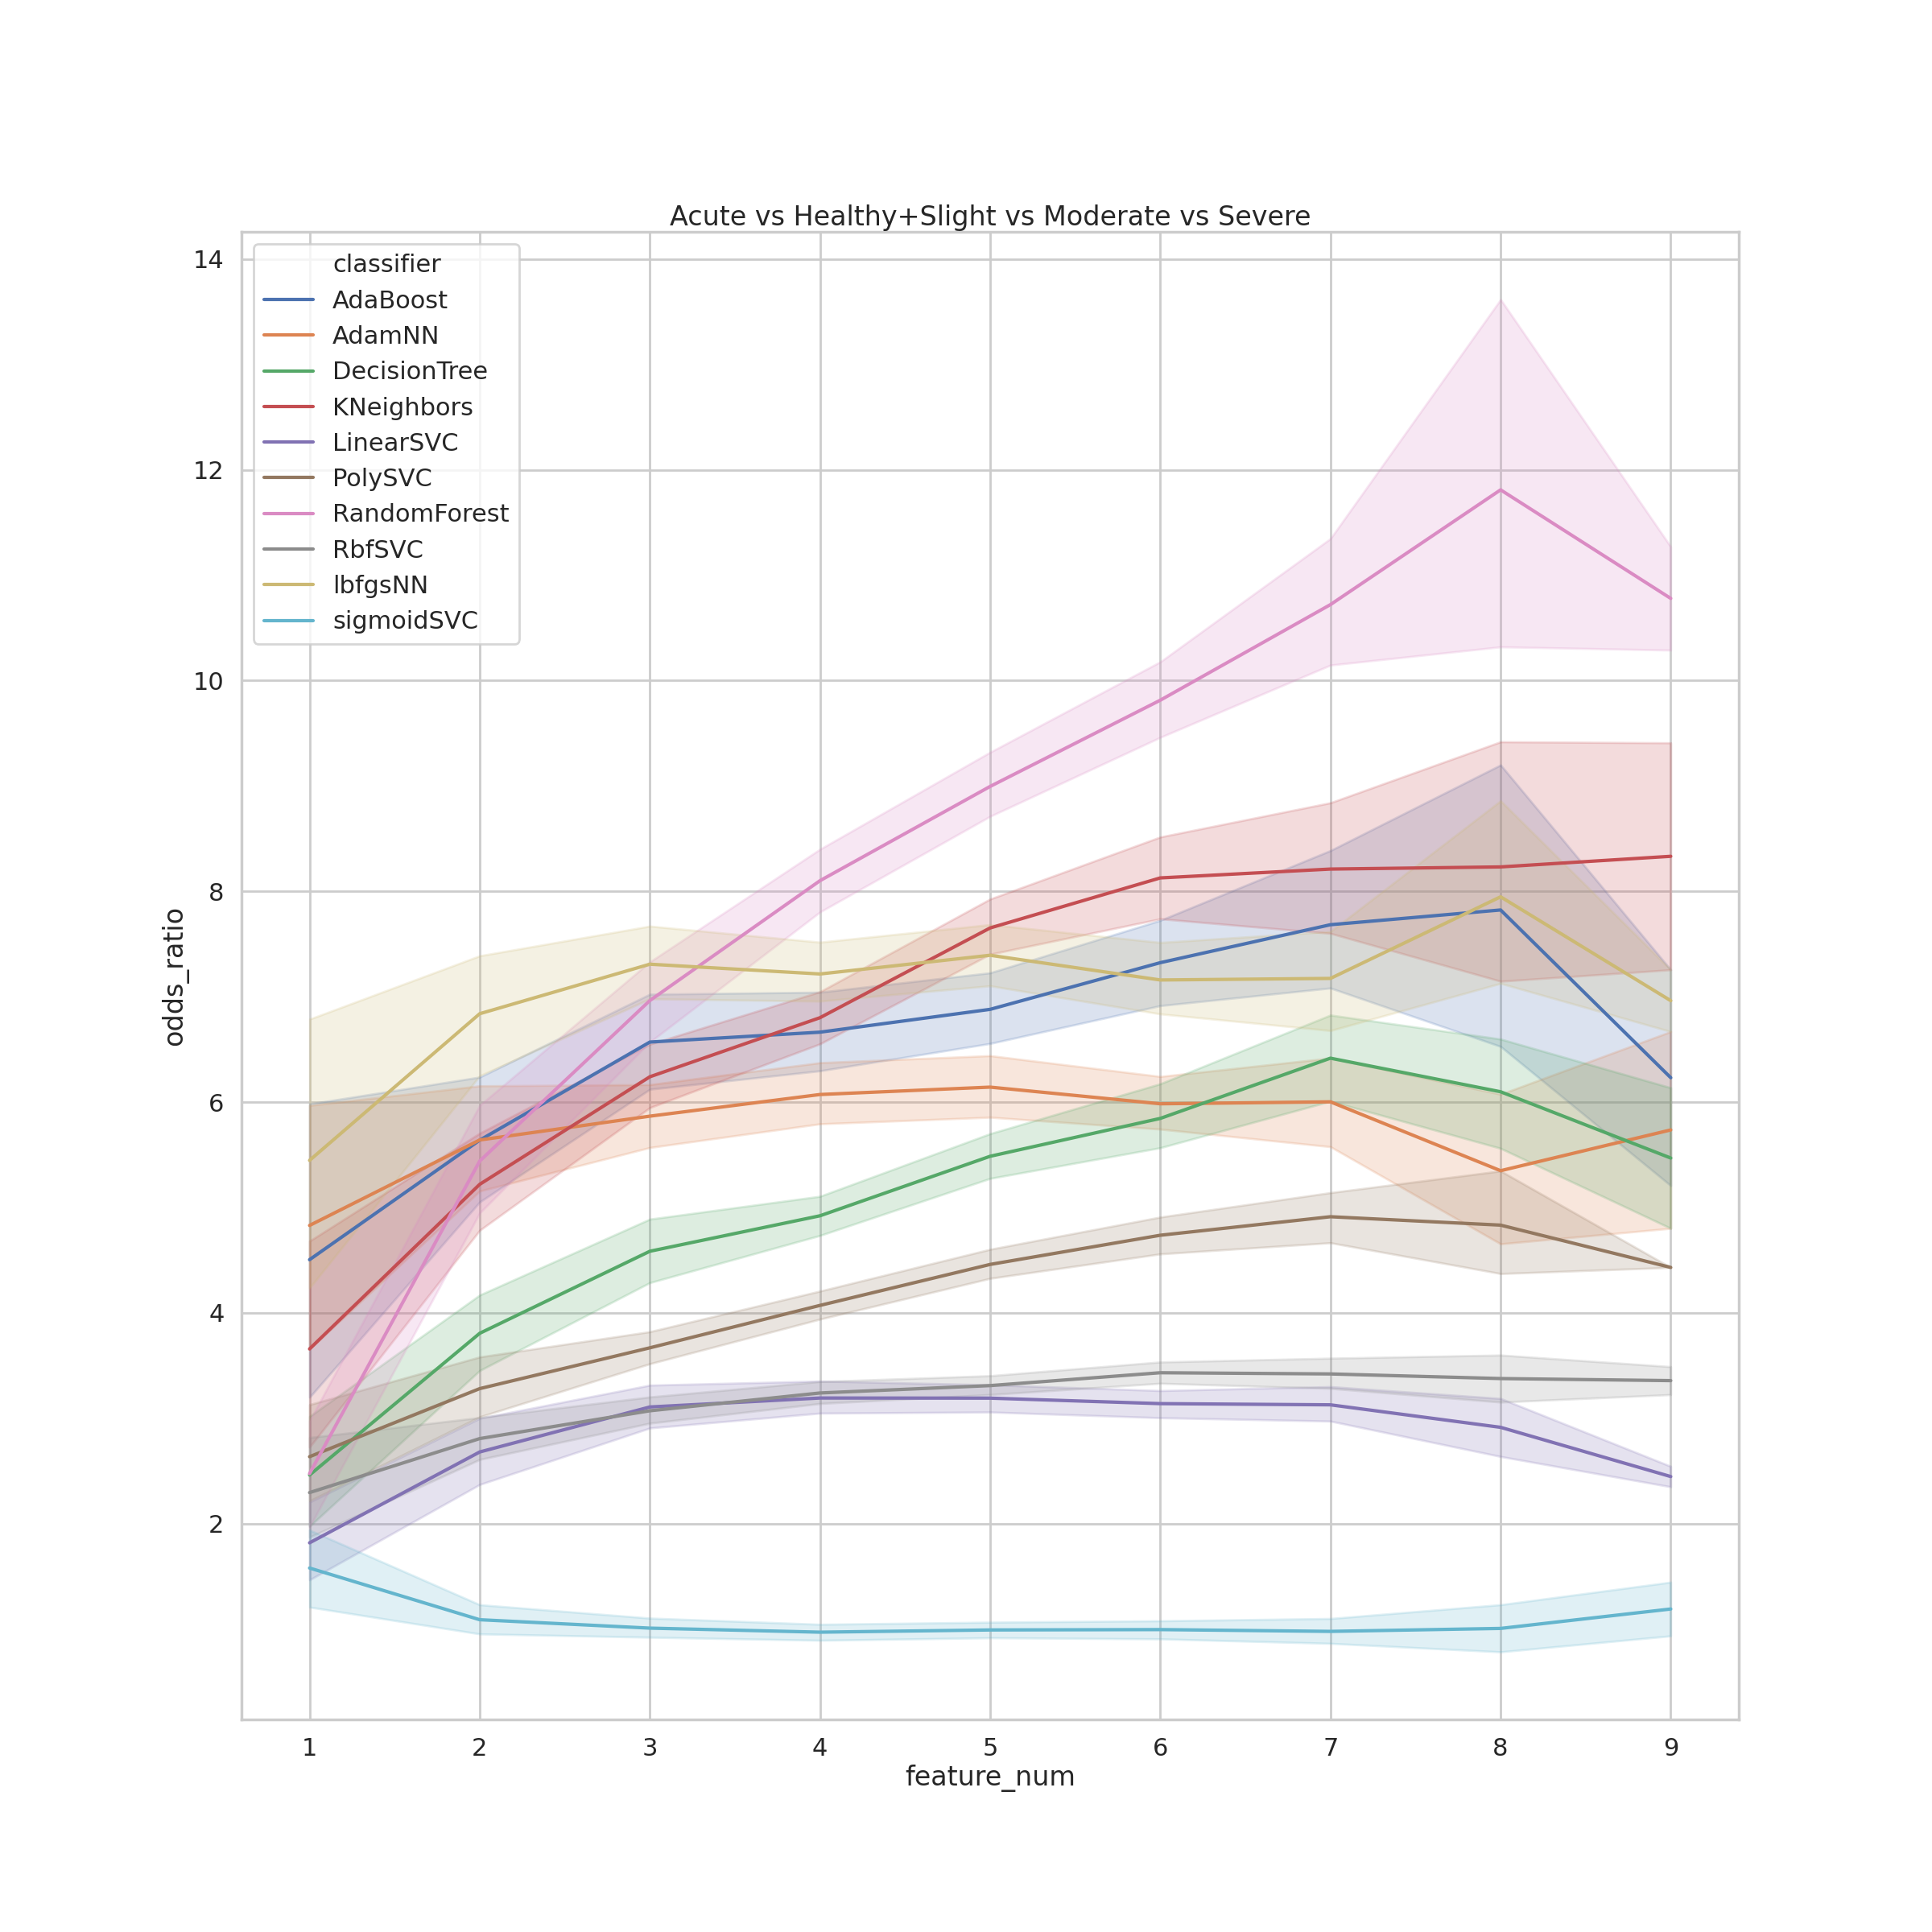
\includegraphics[width=0.3 \linewidth]{figures/Healthy-Slight/odds_ratio.png}
	    				&
	    				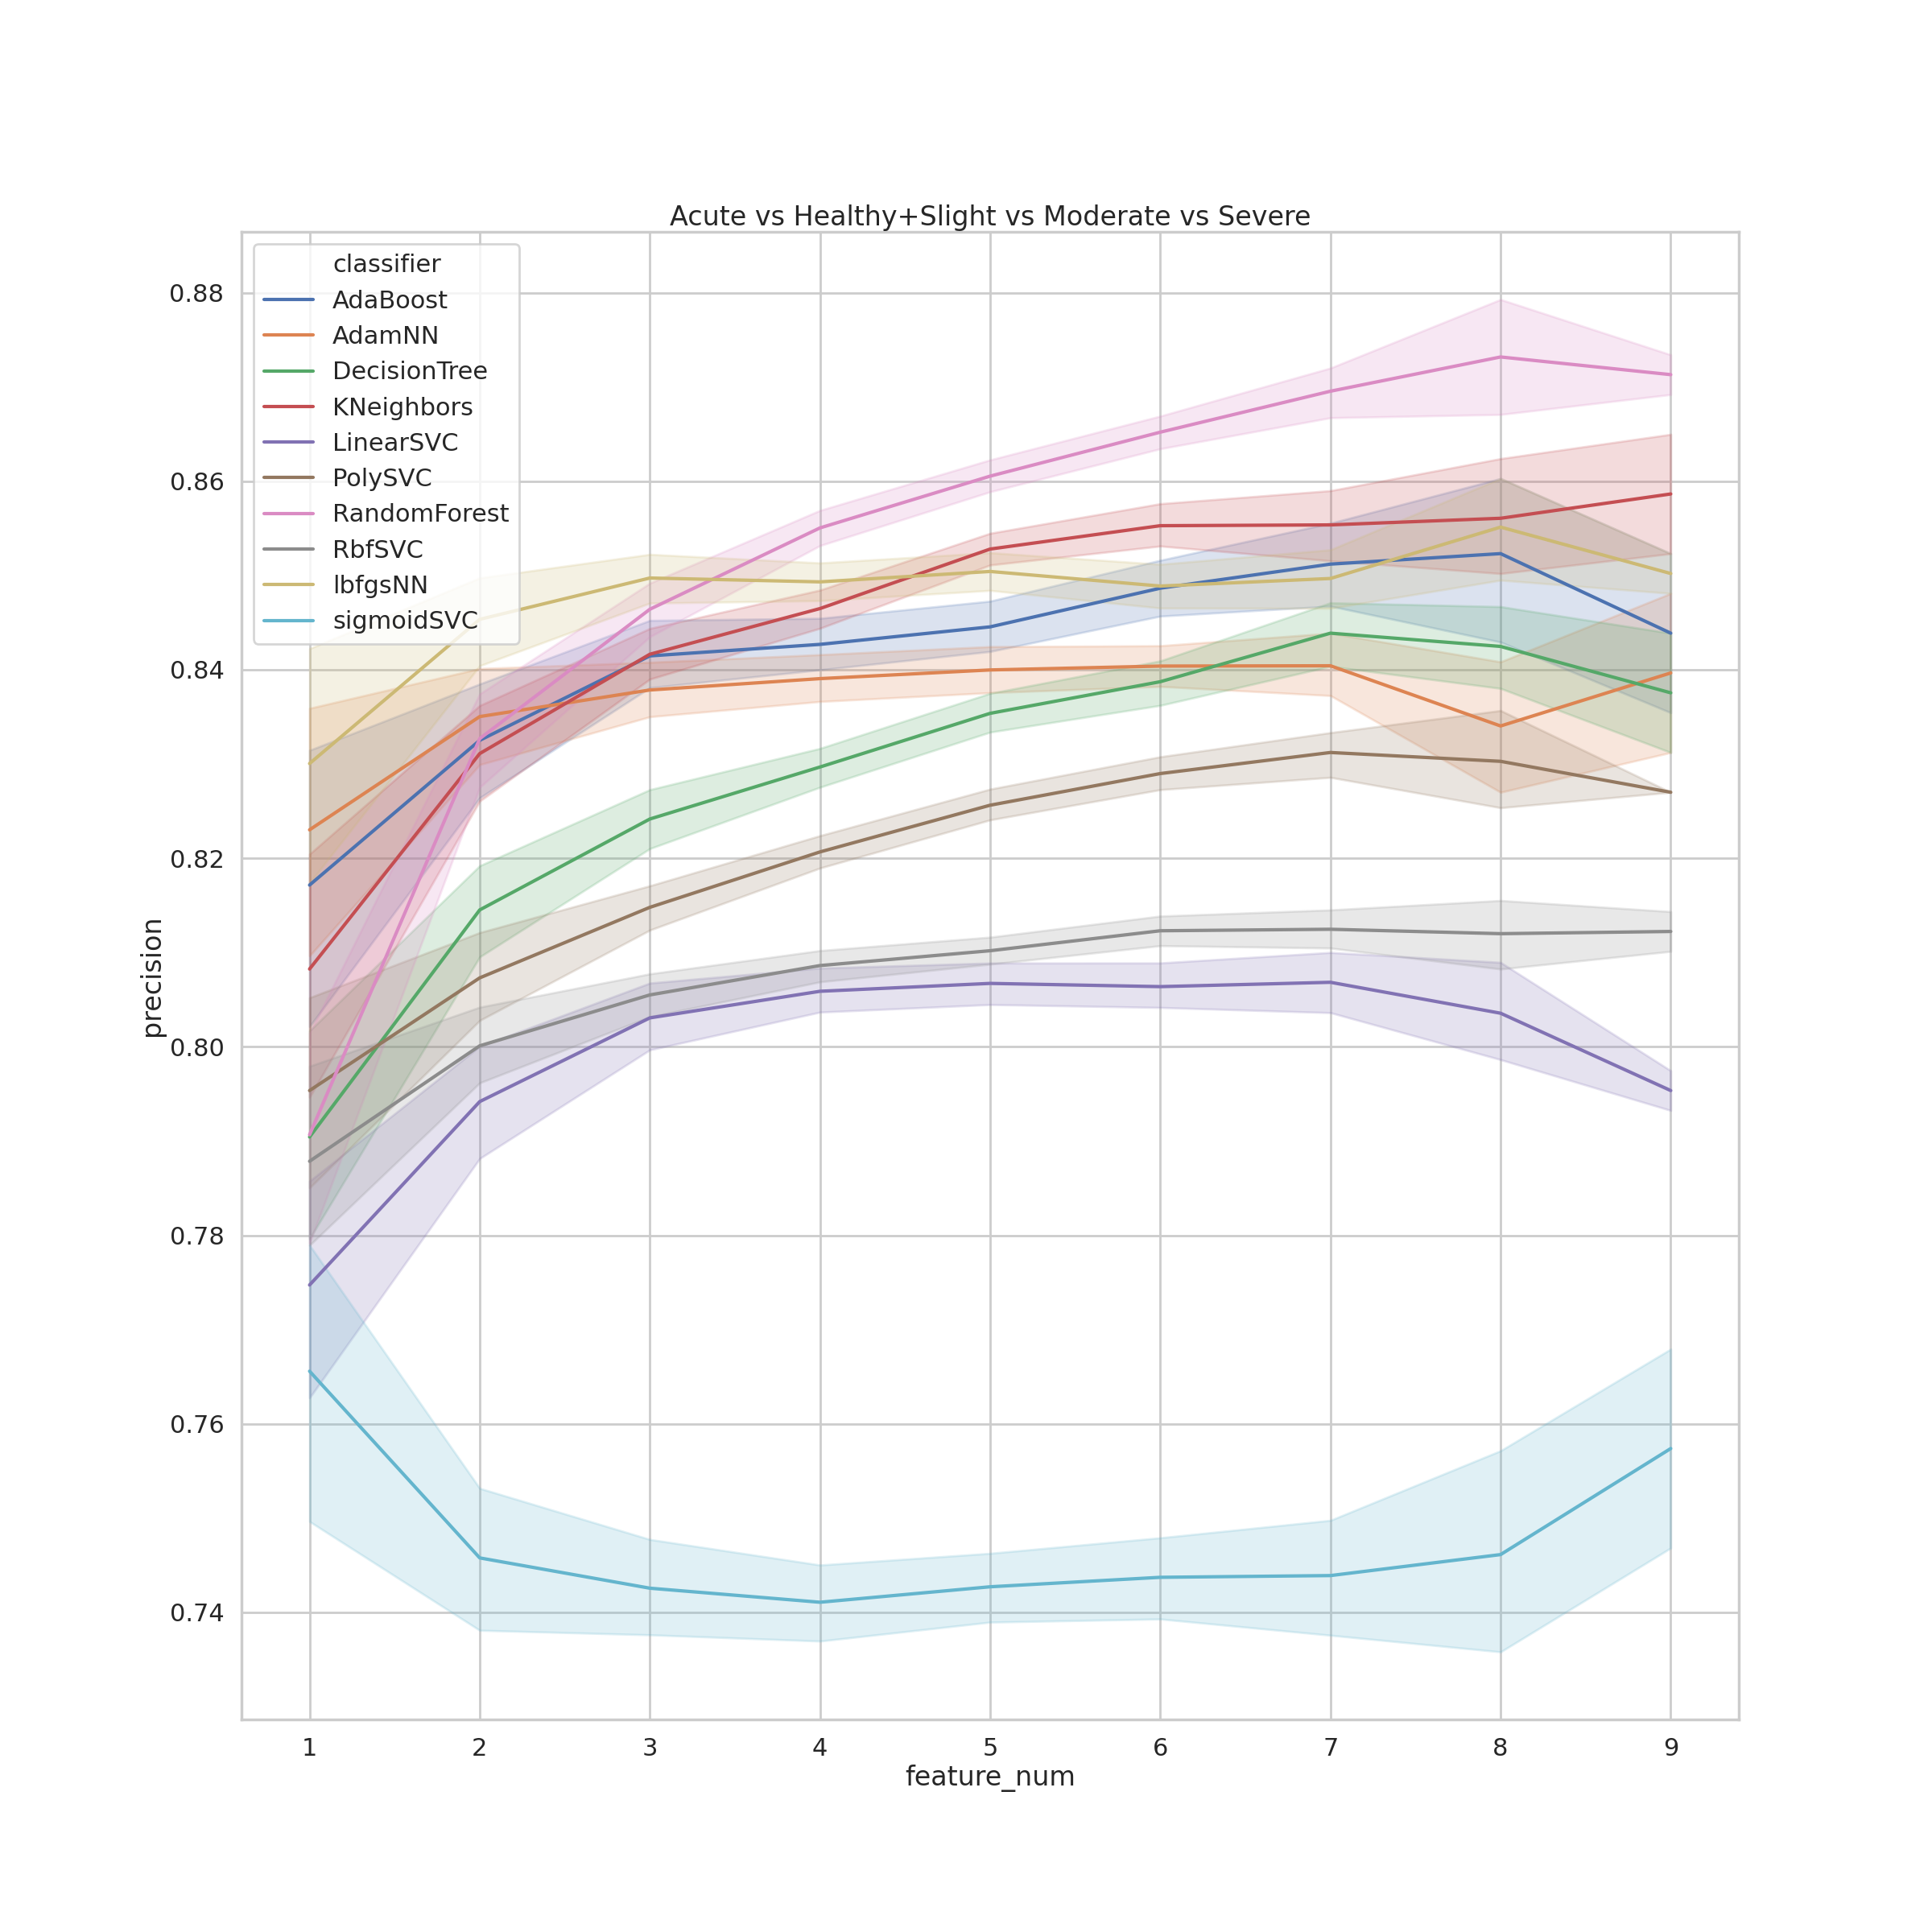
\includegraphics[width=0.3 \linewidth]{figures/Healthy-Slight/precision.png}
	    				\\
	    				\mbox{Negative predictive value} & \mbox{Odds ratio} & \mbox{Precision} \\ 
	    				
	    				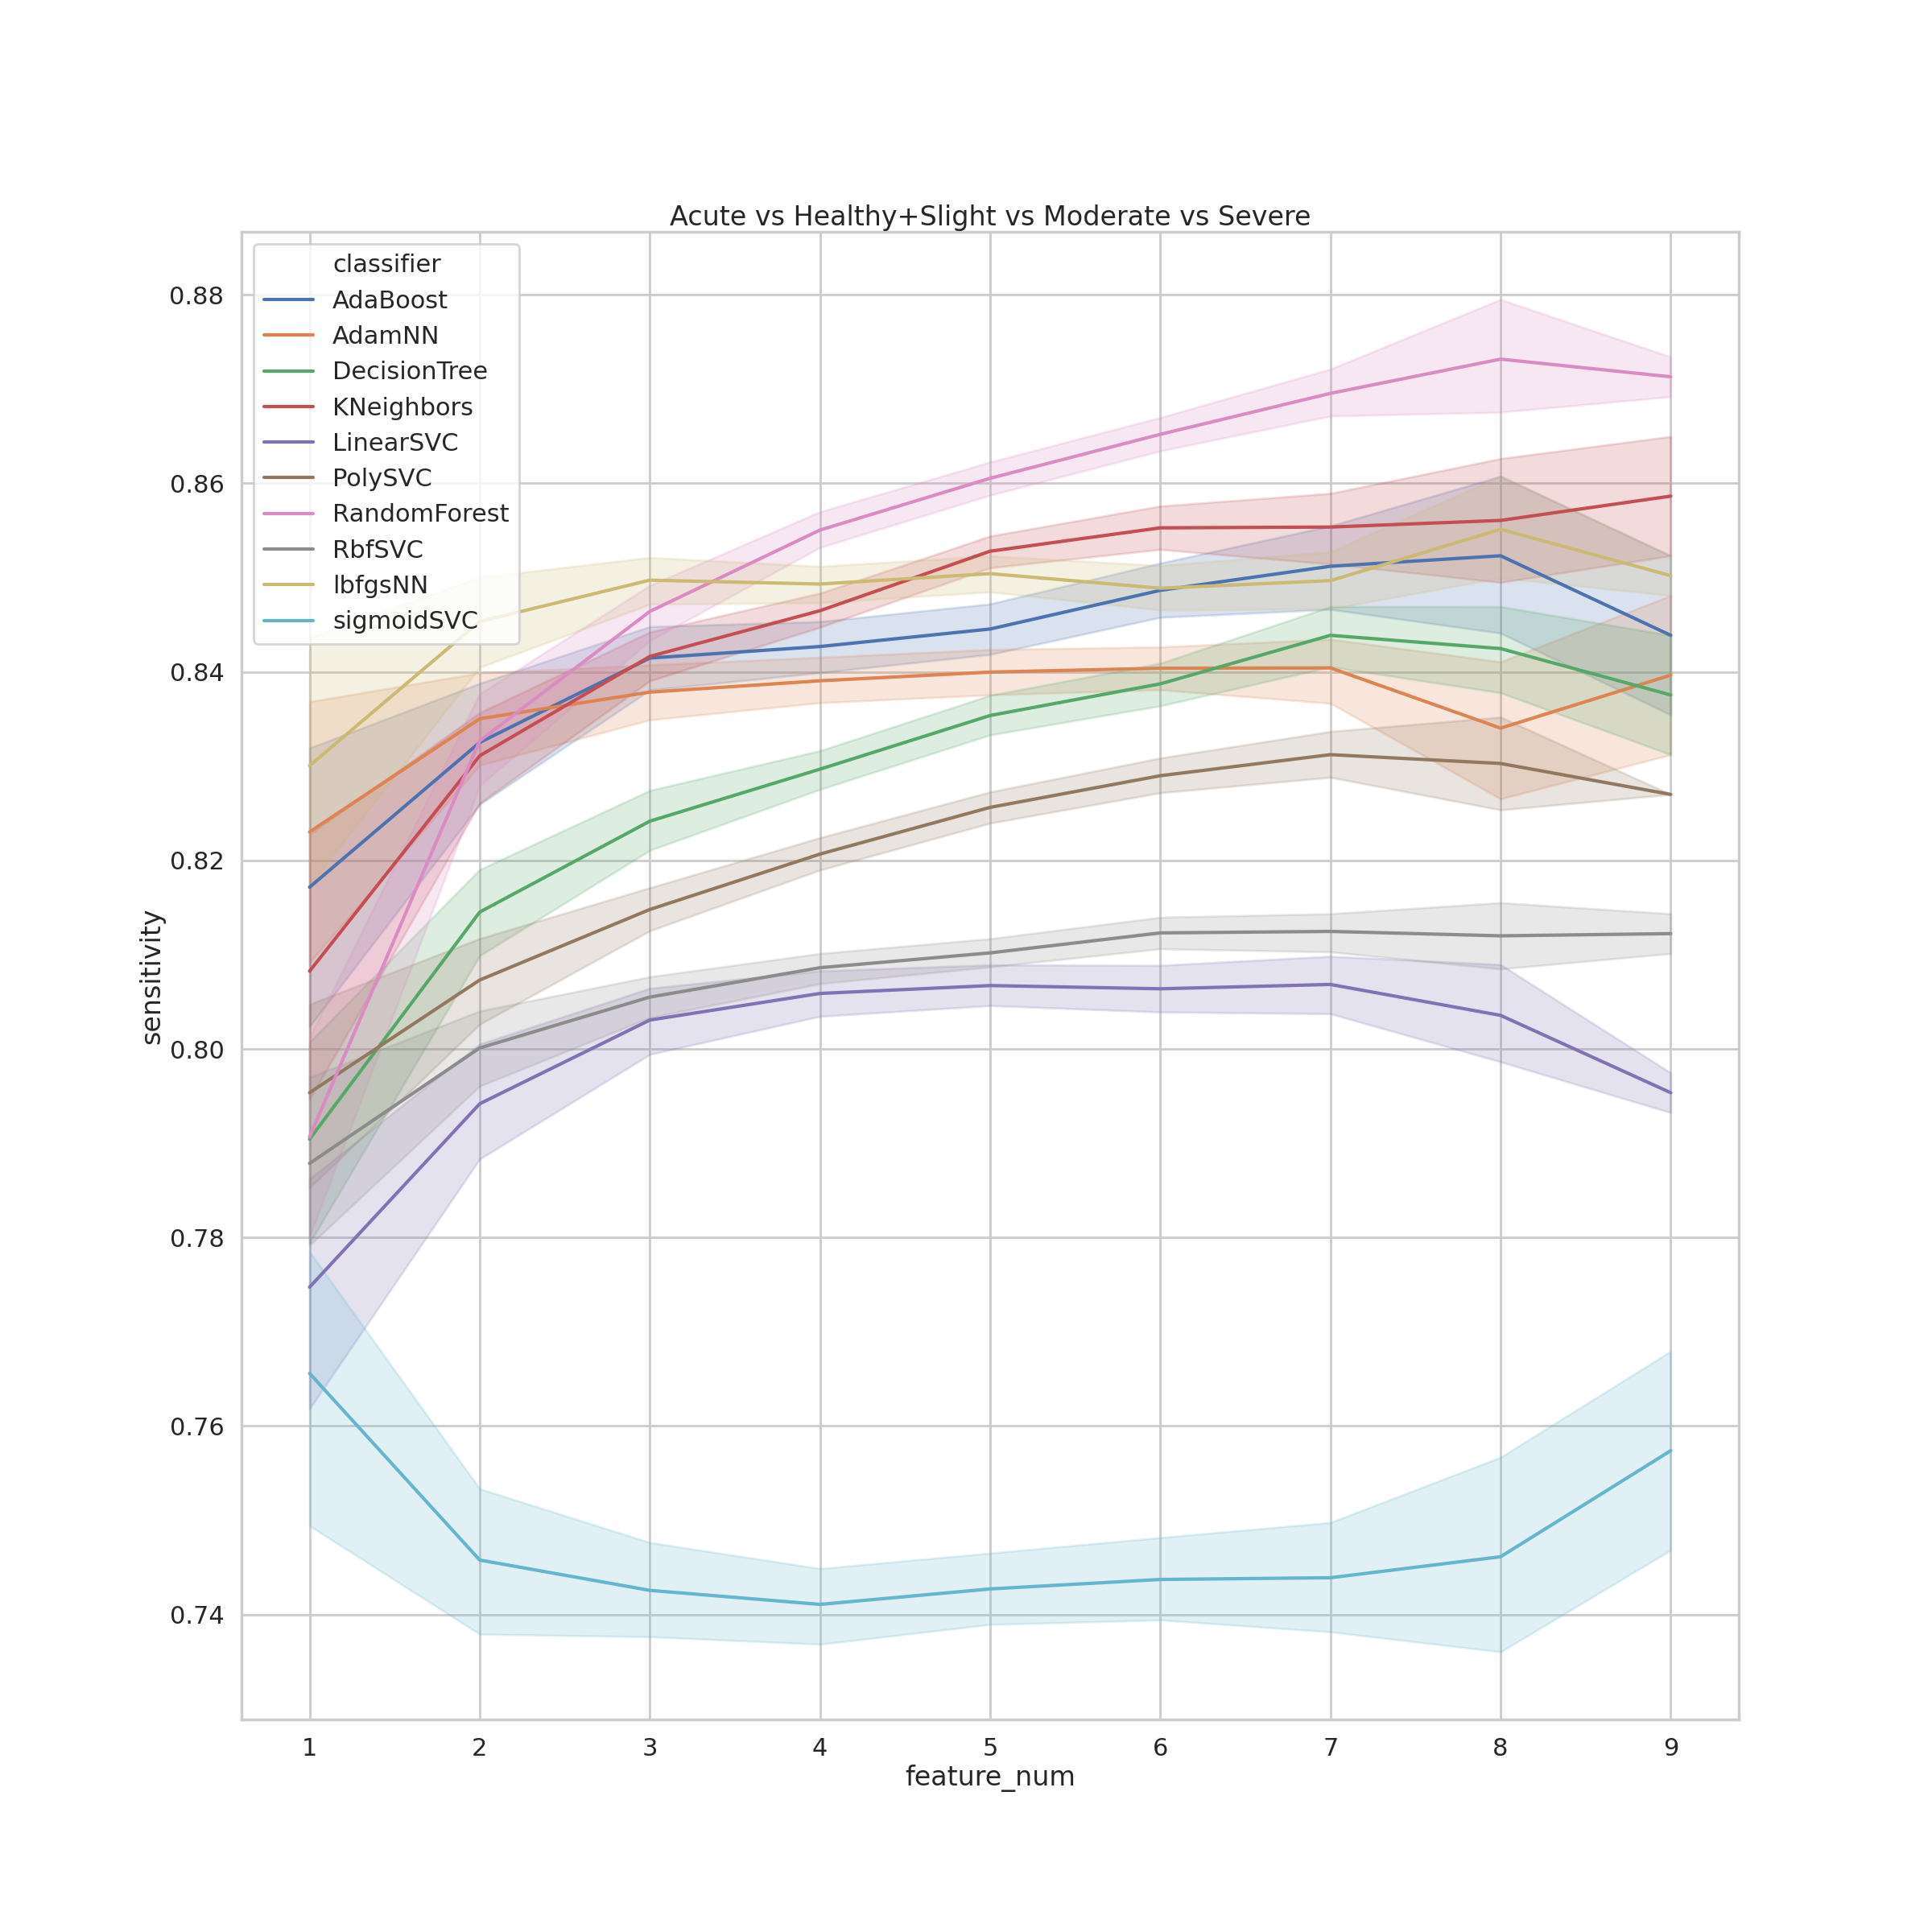
\includegraphics[width=0.3 \linewidth]{figures/Healthy-Slight/sensitivity.png}
	    				&
	    				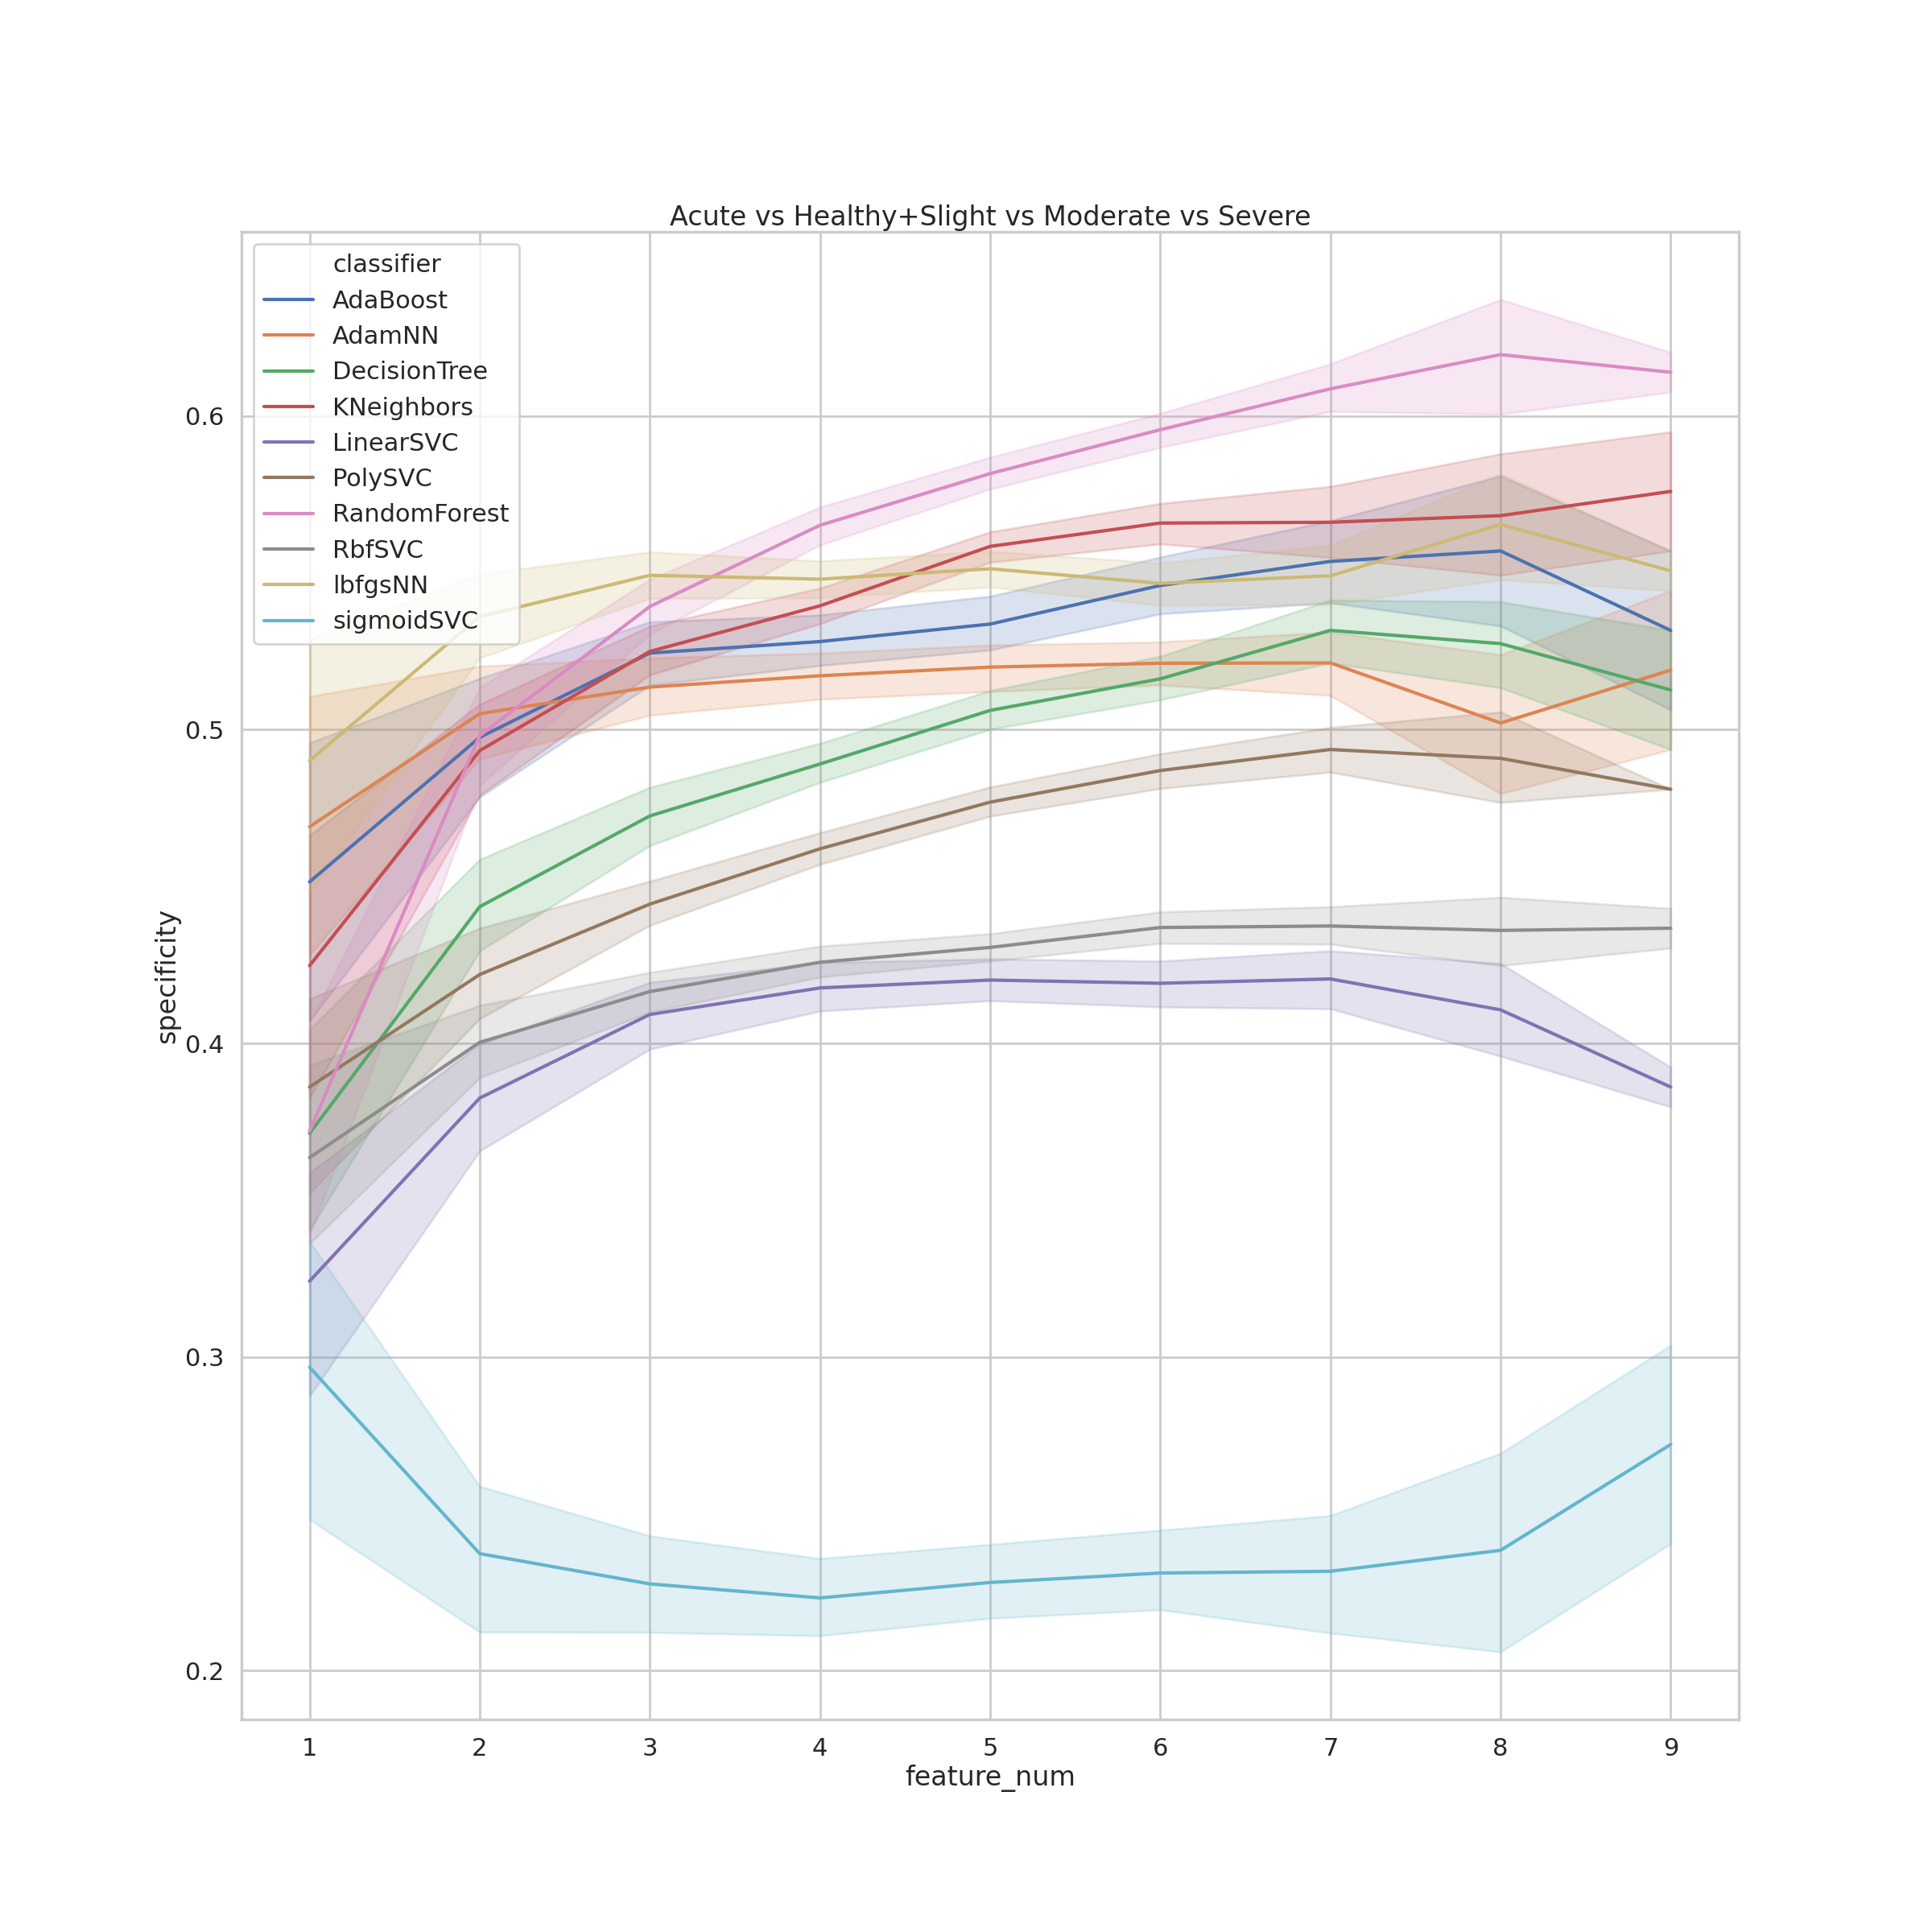
\includegraphics[width=0.3 \linewidth]{figures/Healthy-Slight/specificity.png}
	    				&
	    				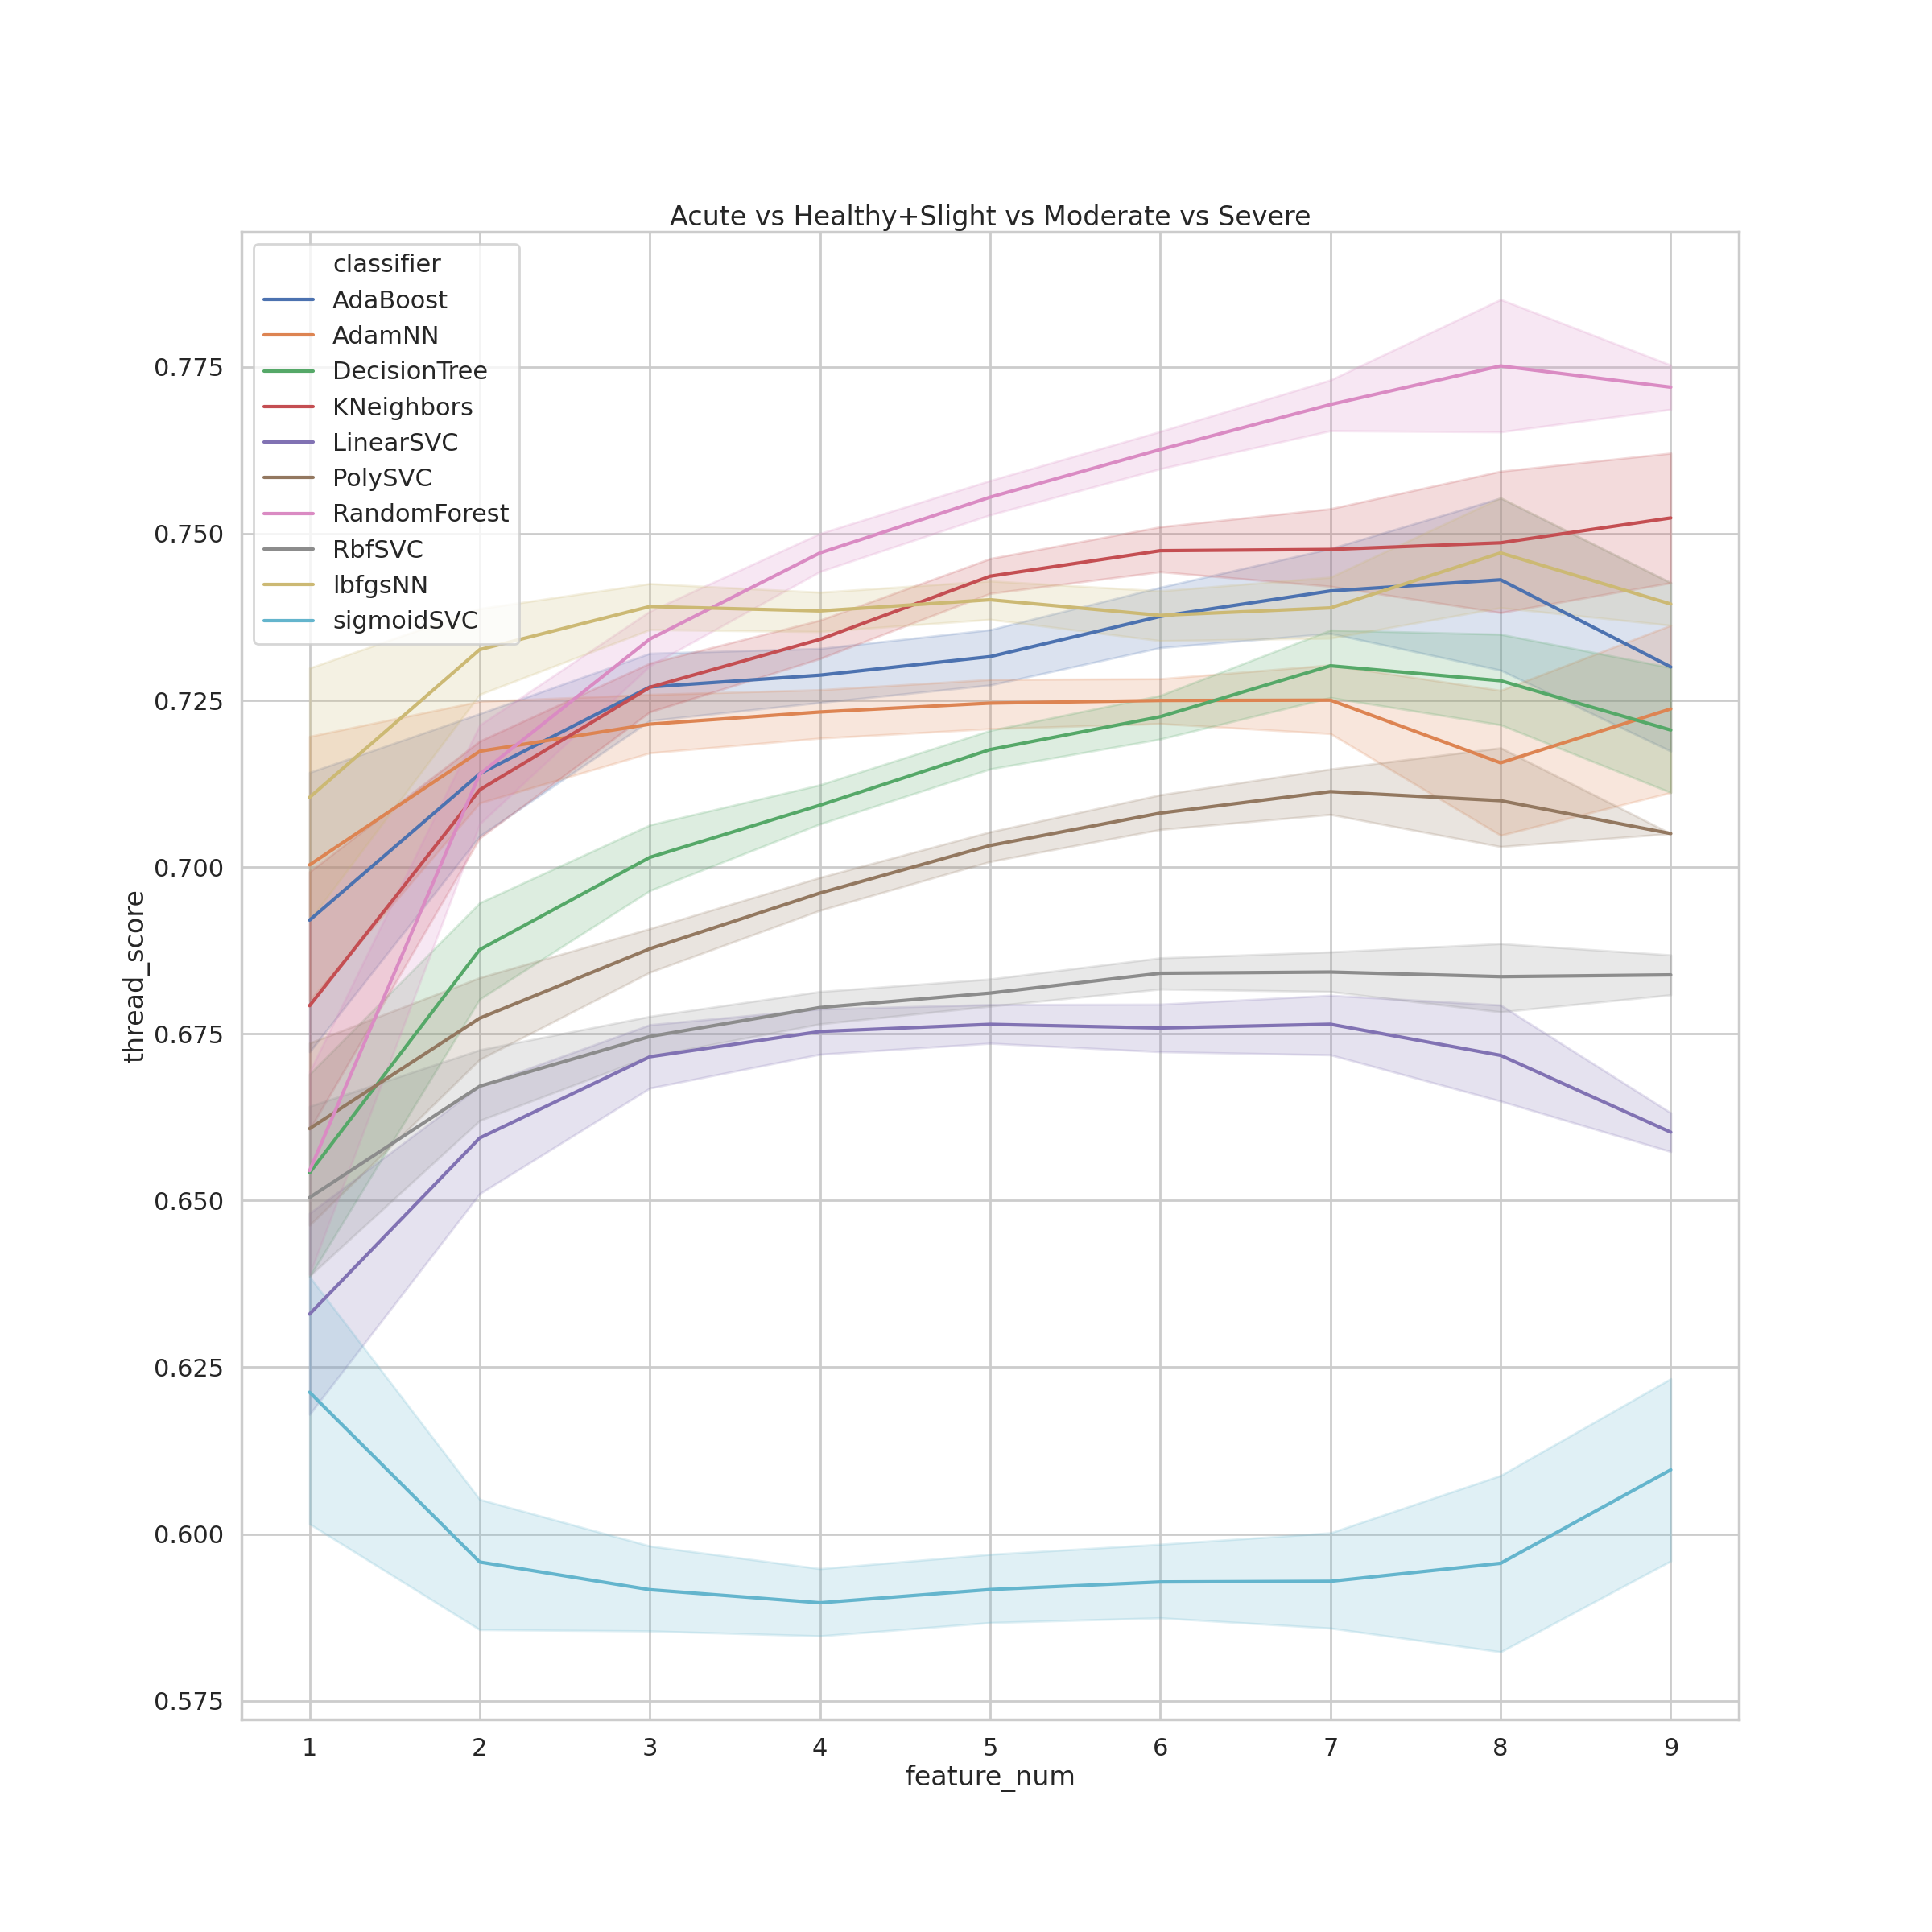
\includegraphics[width=0.3 \linewidth]{figures/Healthy-Slight/thread_score.png}
	    				\\
	    				\mbox{Sensitivity} & \mbox{Specificity} & \mbox{Thread score} \\
	    			\end{array}$
	    			\caption{Confusion Matrix Derivations from Merged Healthy-Slight Classification}
	    			\label{fig:h-sli-confusion}
    			\end{figure}
    			
    			\begin{figure}[htbp]
    				\centering
					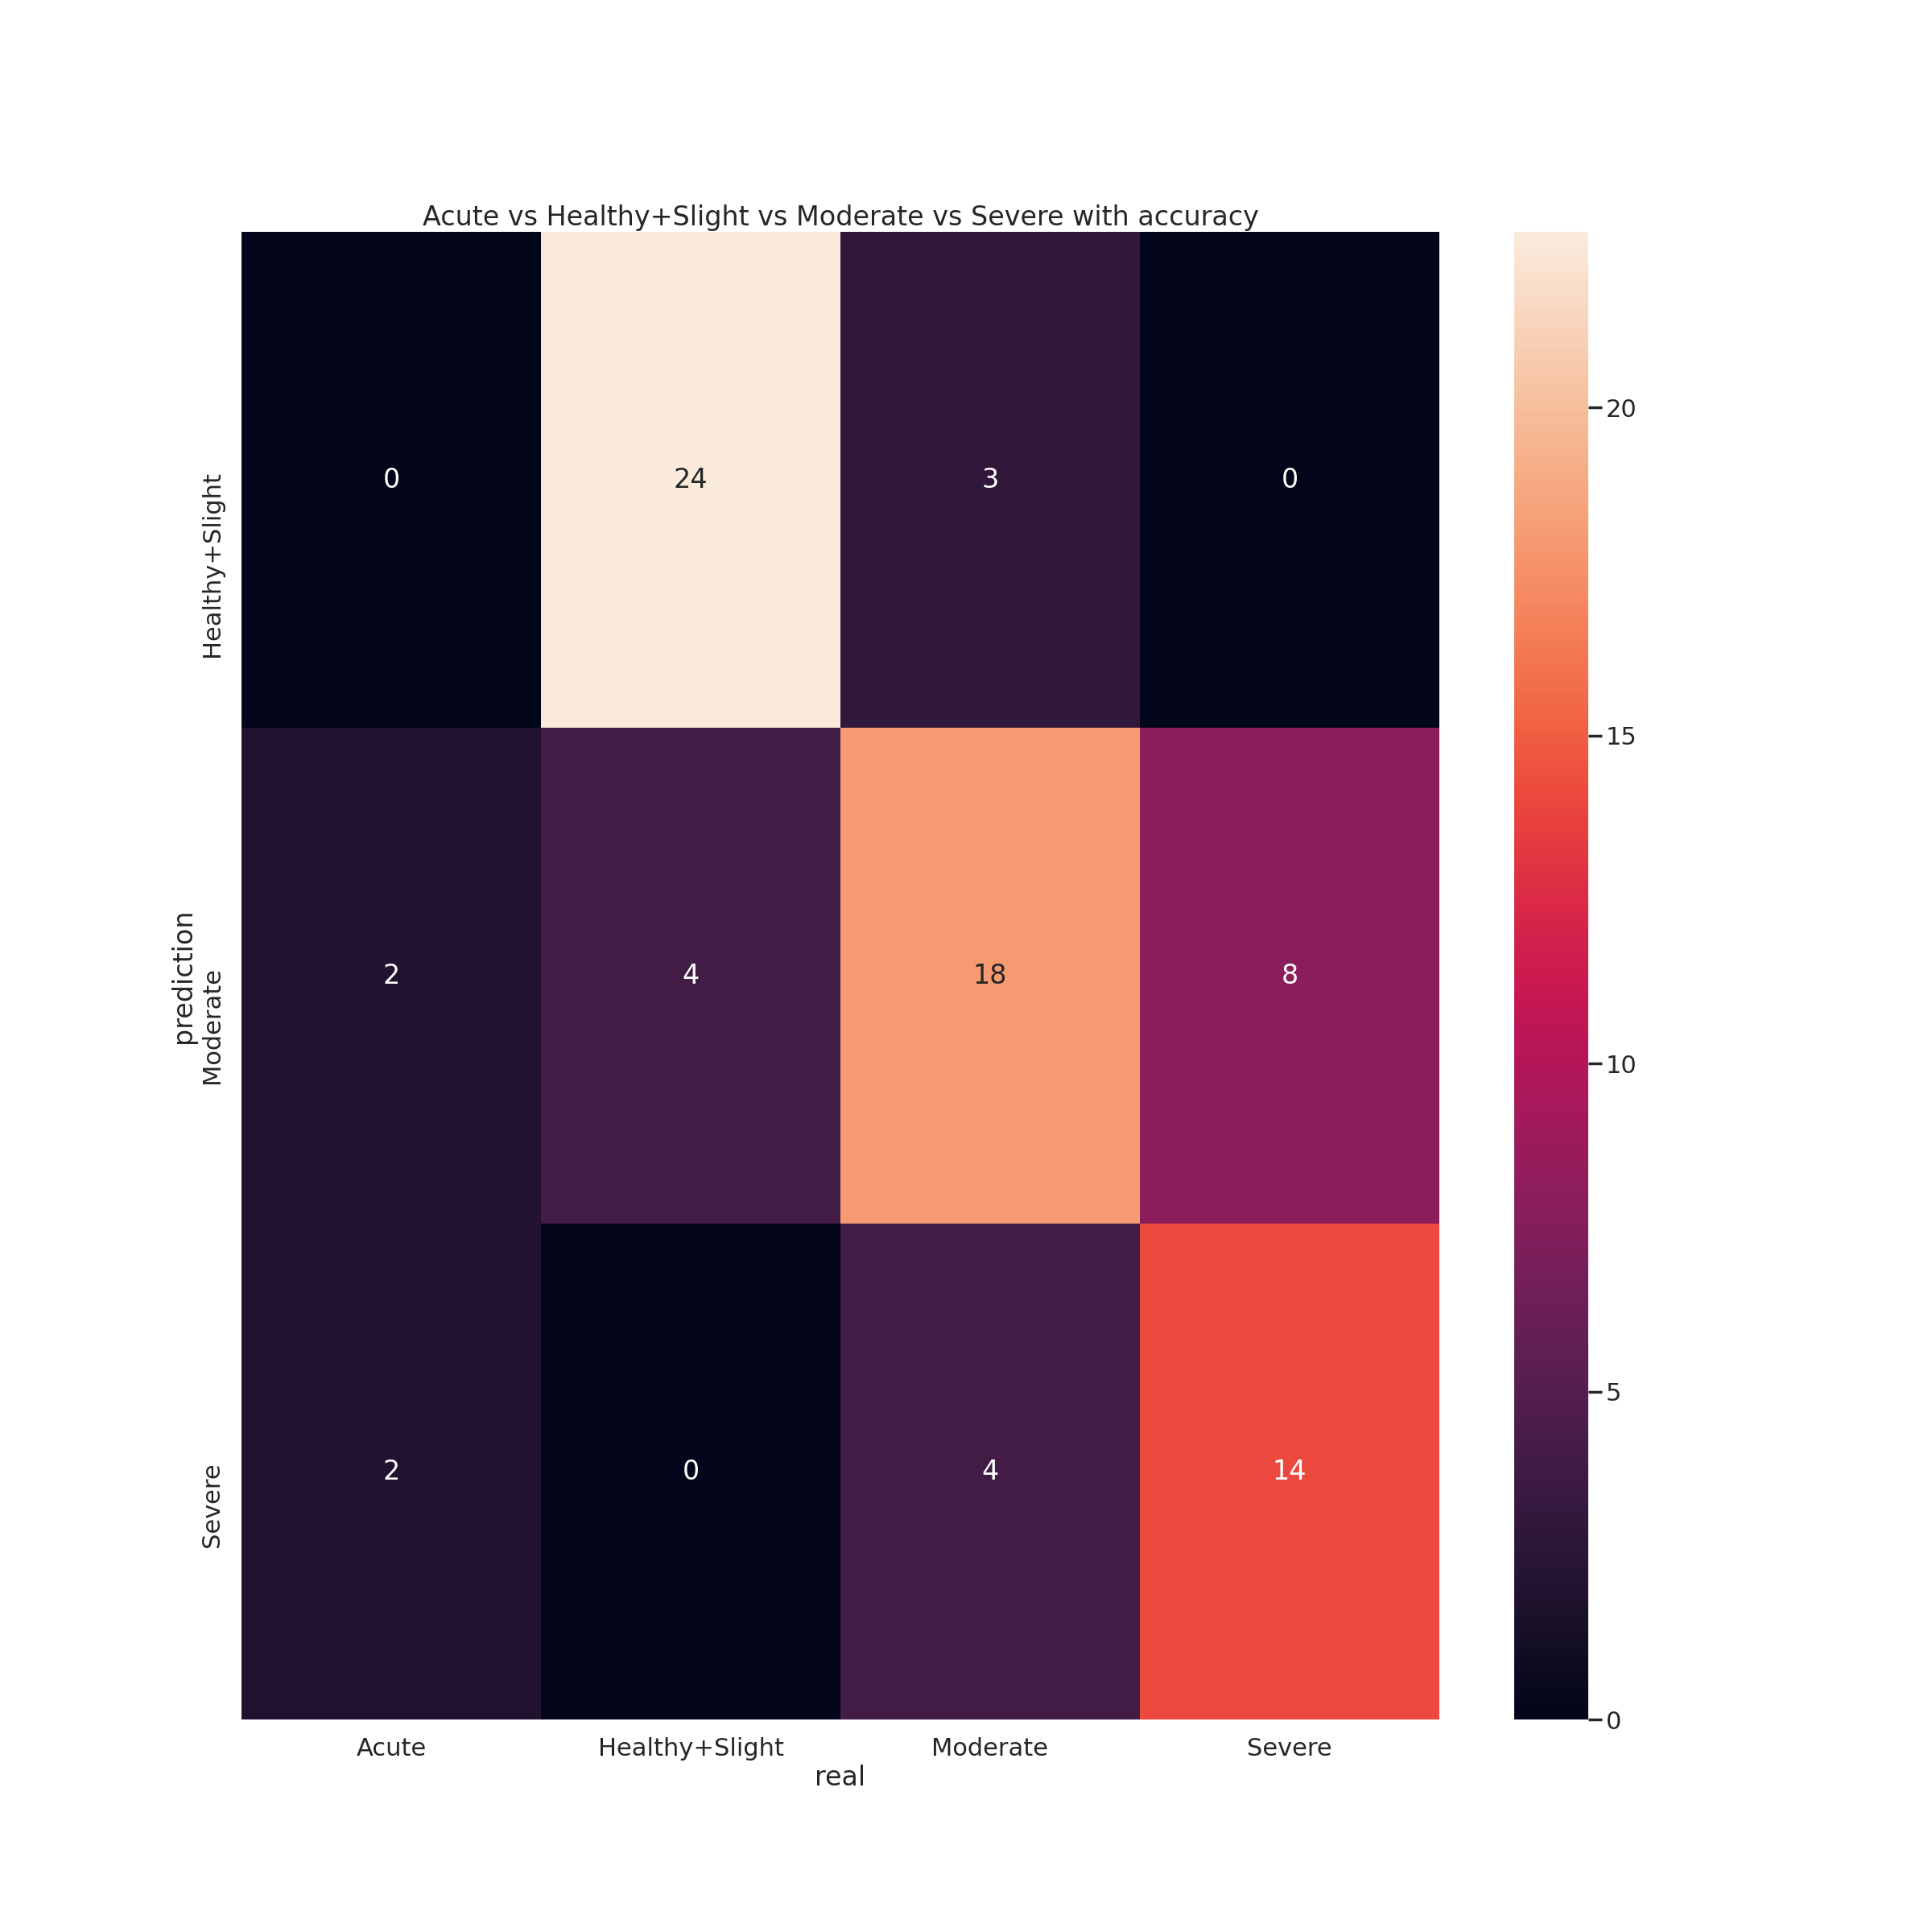
\includegraphics[width=0.5 \linewidth]{figures/Healthy-Slight/heatmap.png}
					\caption{Heatmap Plot for Merged Healthy-Slight Classification with Random Forest}
					\label{fig:h-sli-heatmap}
    			\end{figure}
    		
    		\subsubsection{Merged Slight-Moderate Class}
    			Figure \ref{fig:sli-m-confusion} displays the derivations of confusion matrix in merged slight-moderate classification. Note that the values in figure \ref{fig:sli-m-confusion}, mean values from combination which used same number of features will be shown. As figure \ref{fig:sli-m-confusion}, the K-Neighbor algorithm has the best values with all features.
    			
			   	\begin{figure}[htbp]
    				\centering
    				$\begin{array}{ccc}
	    				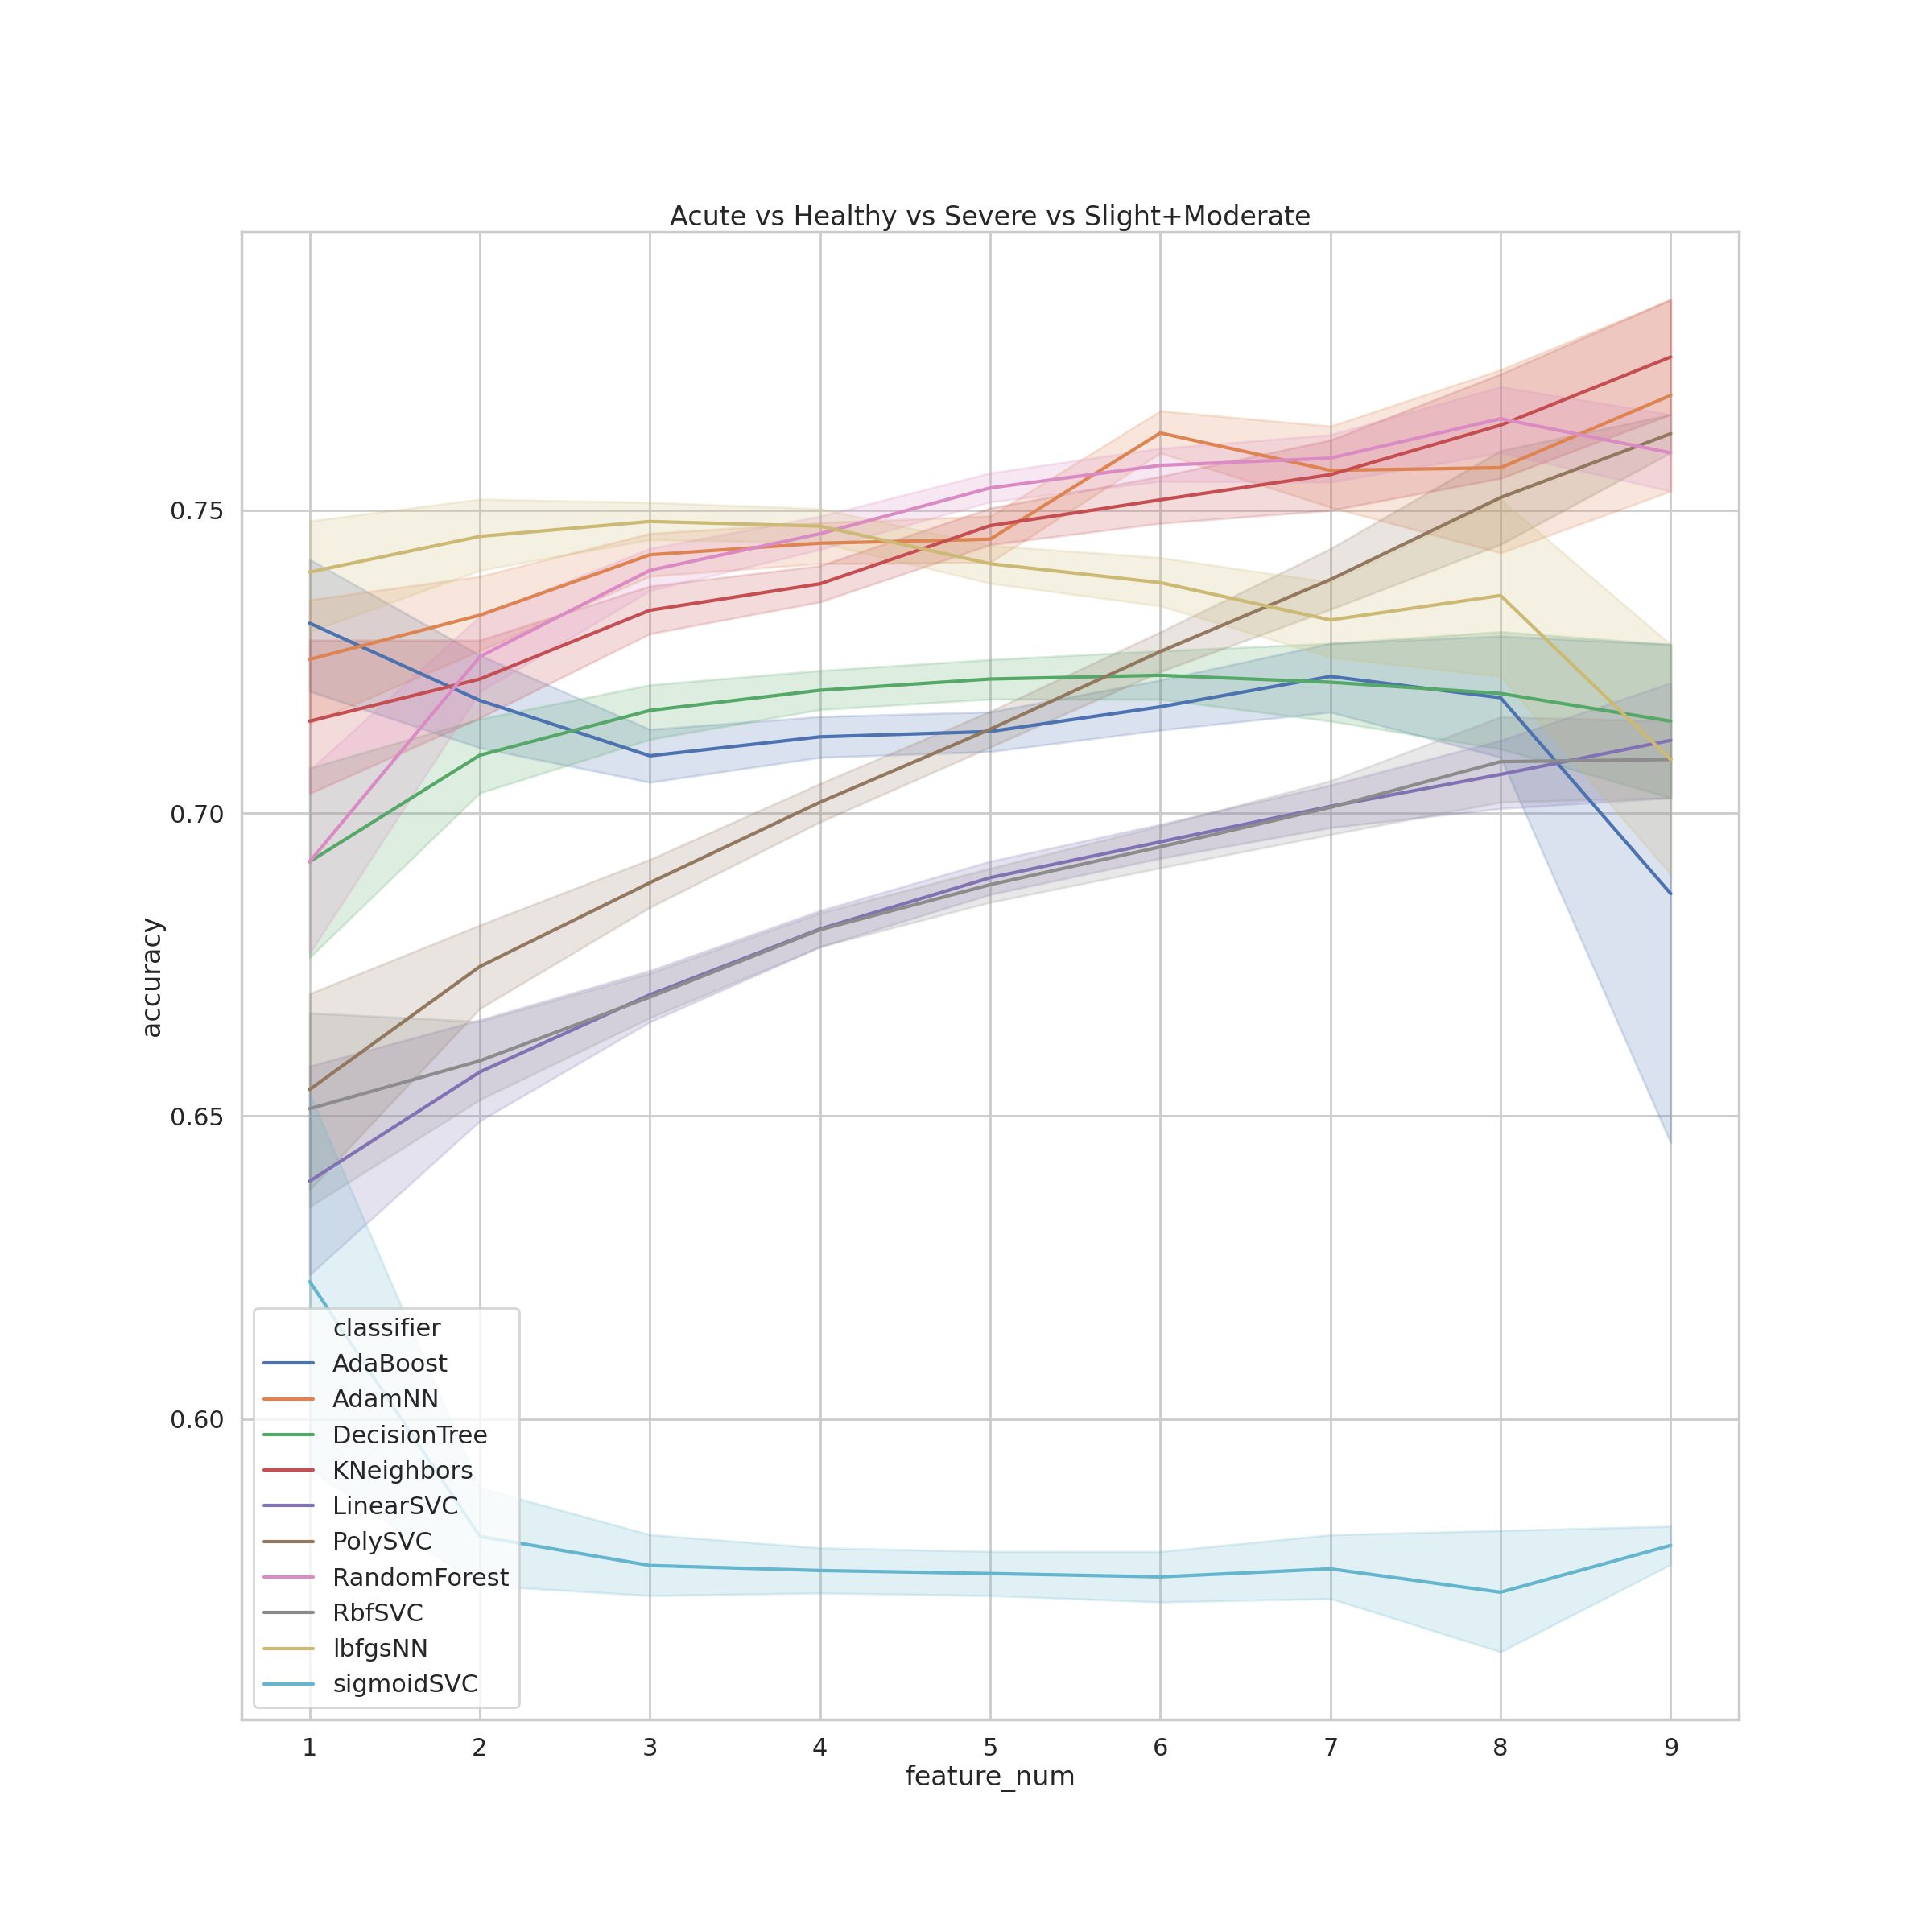
\includegraphics[width=0.3 \linewidth]{figures/Slight-Moderate/accuracy.png}
	    				&
	    				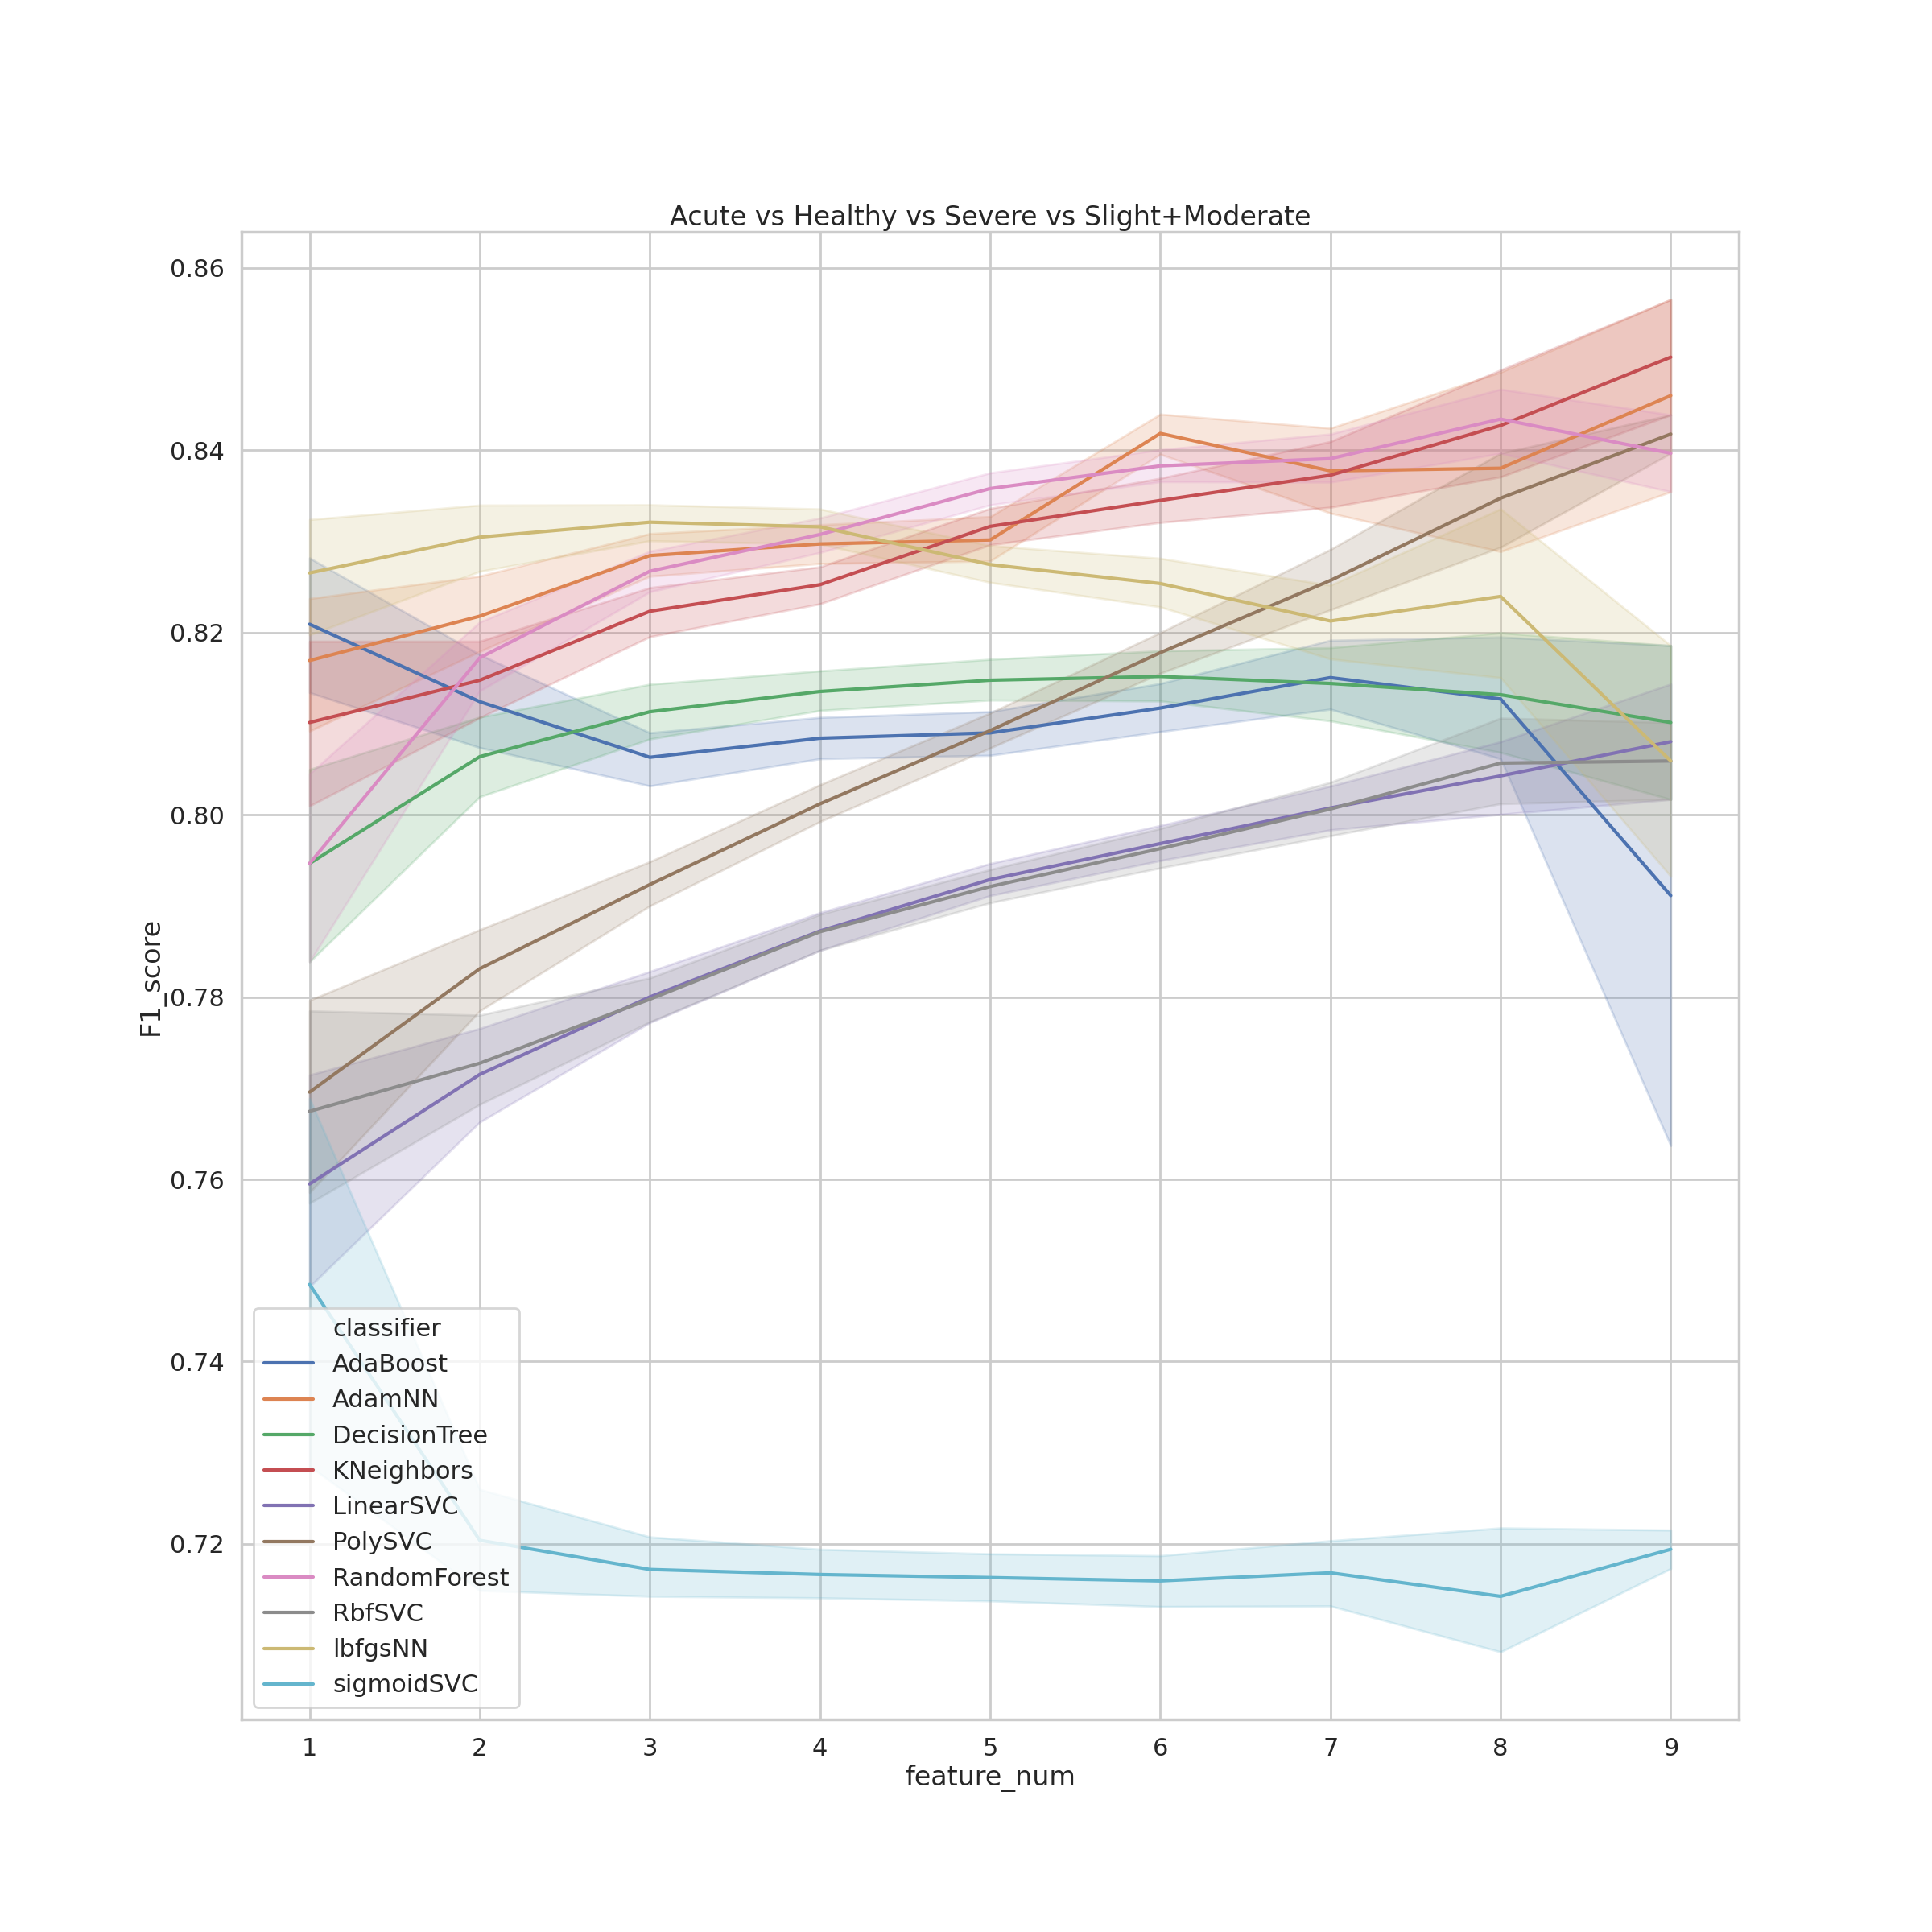
\includegraphics[width=0.3 \linewidth]{figures/Slight-Moderate/F1_score.png}
	    				&
	    				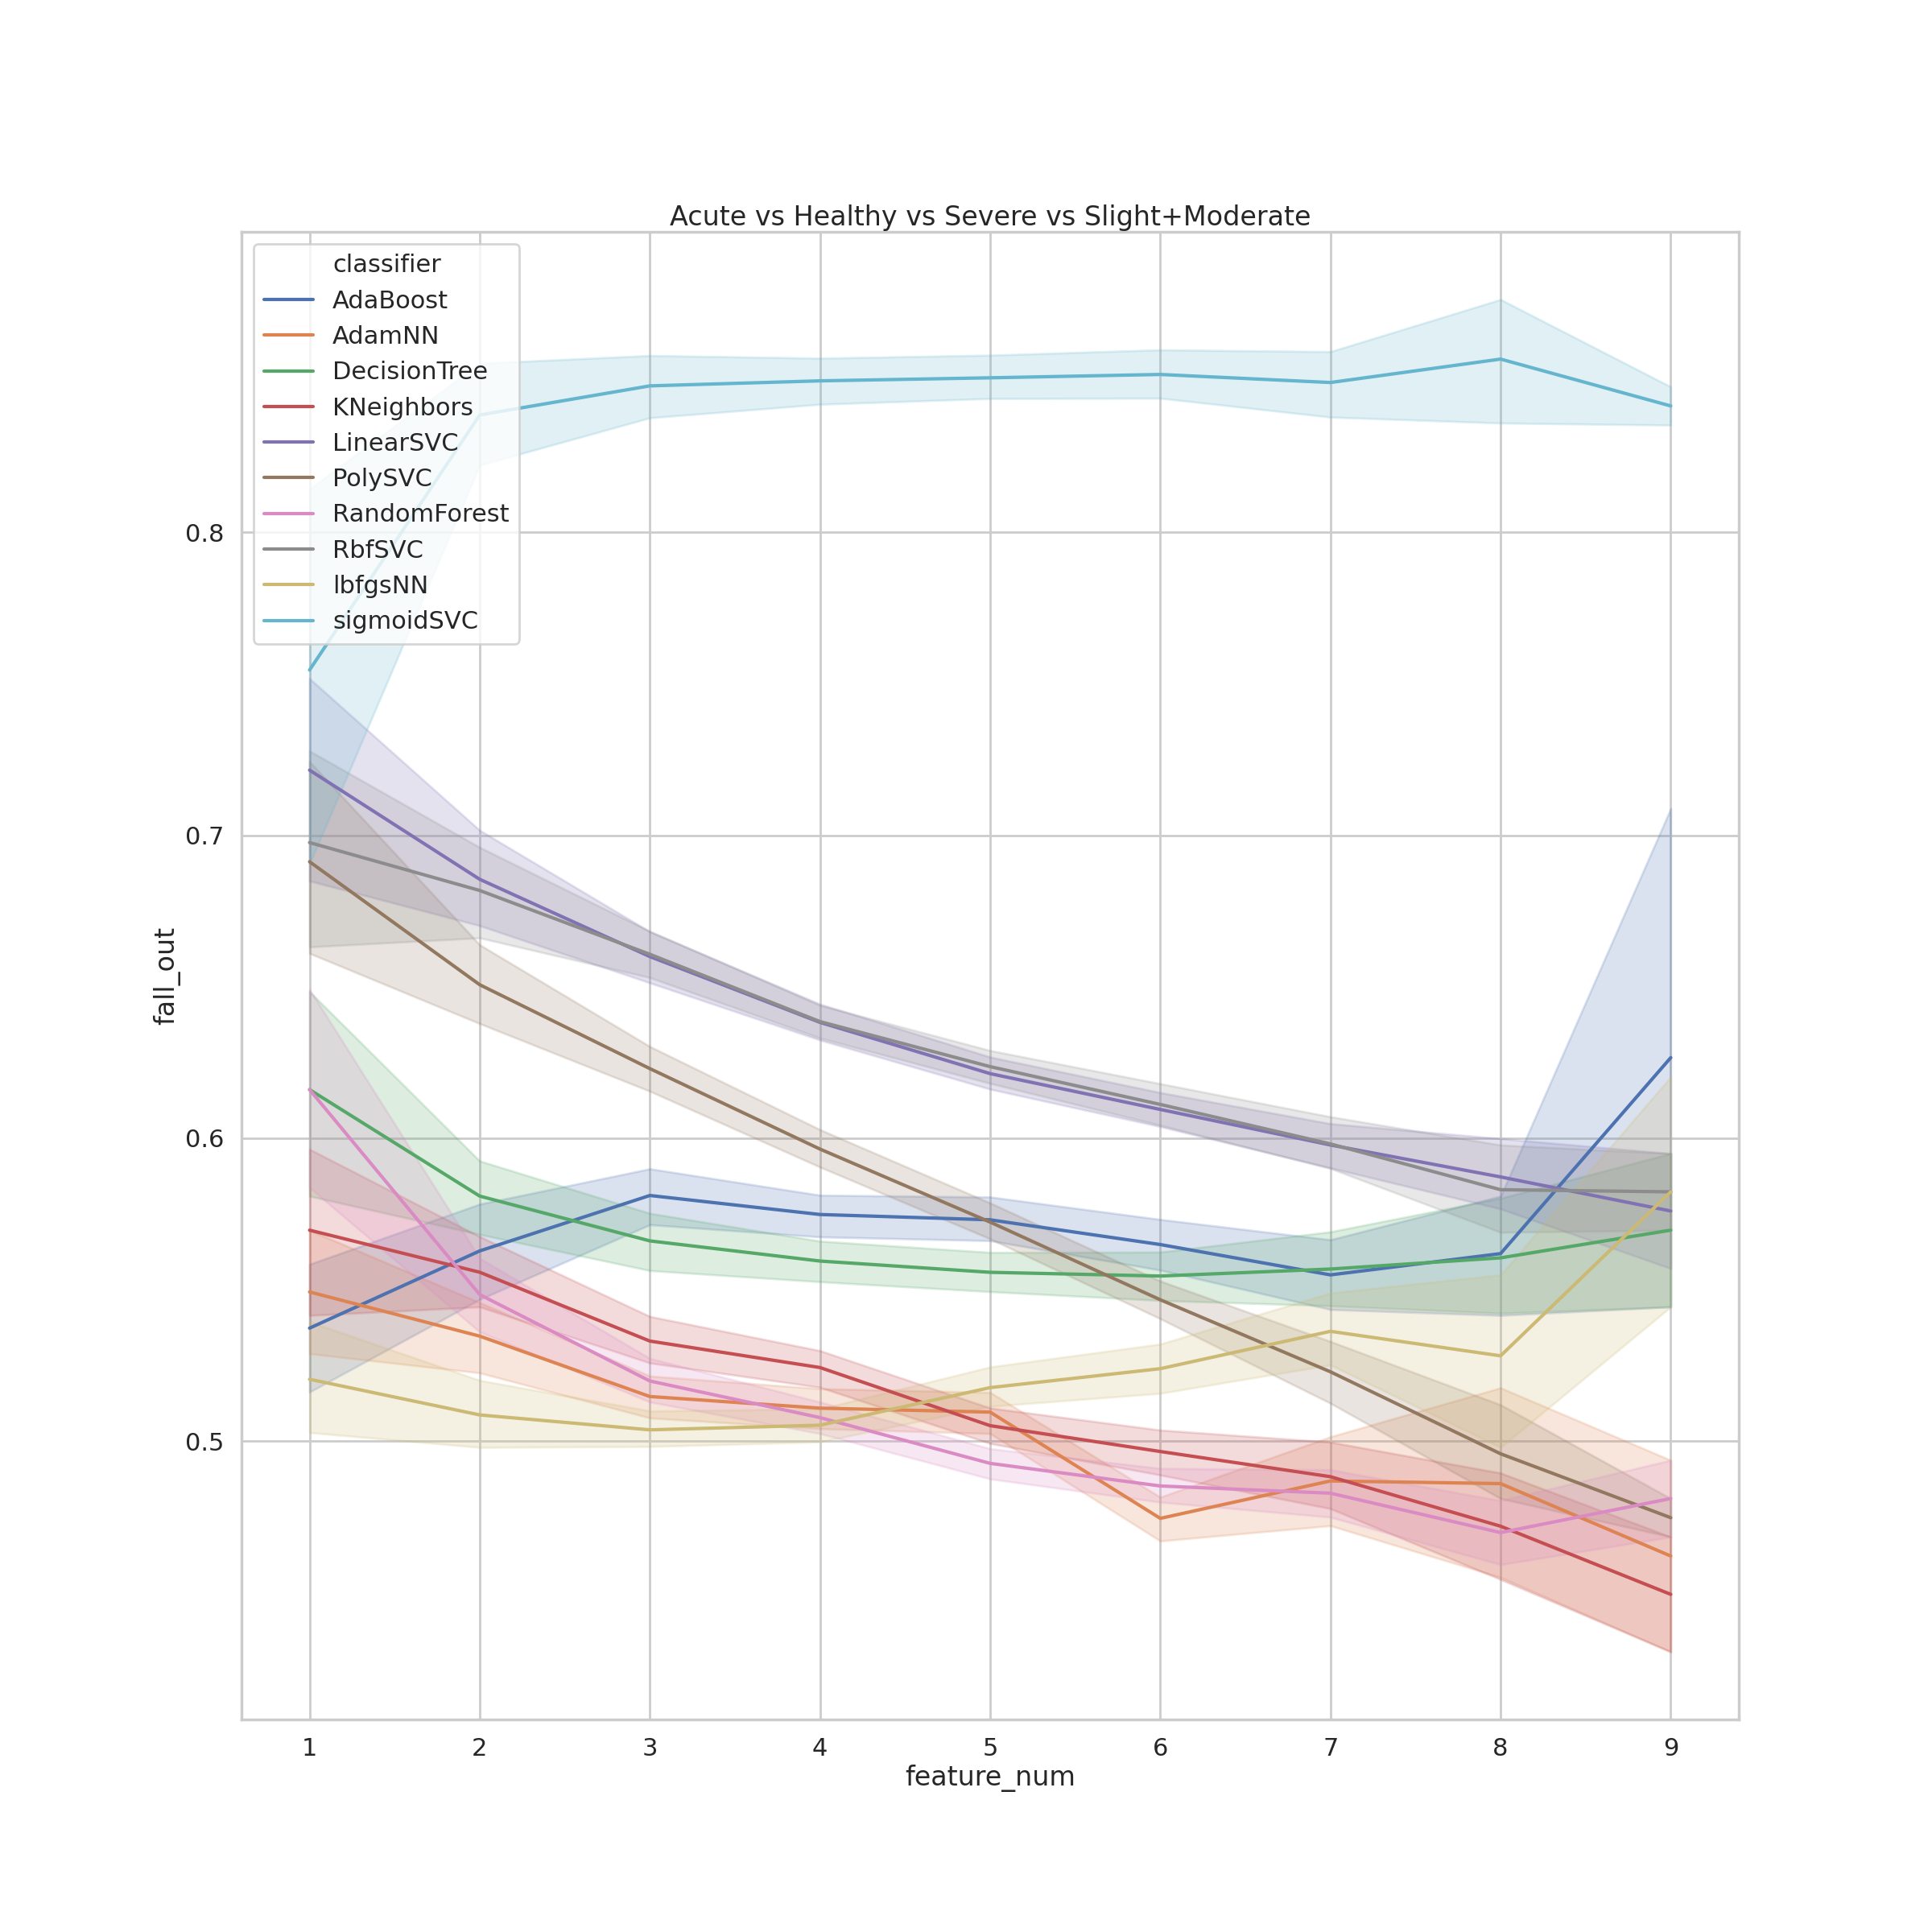
\includegraphics[width=0.3 \linewidth]{figures/Slight-Moderate/fall_out.png}
	    				\\
	    				\mbox{Accuracy} & \mbox{F1 score} & \mbox{Fall-out} \\
	    				
	    				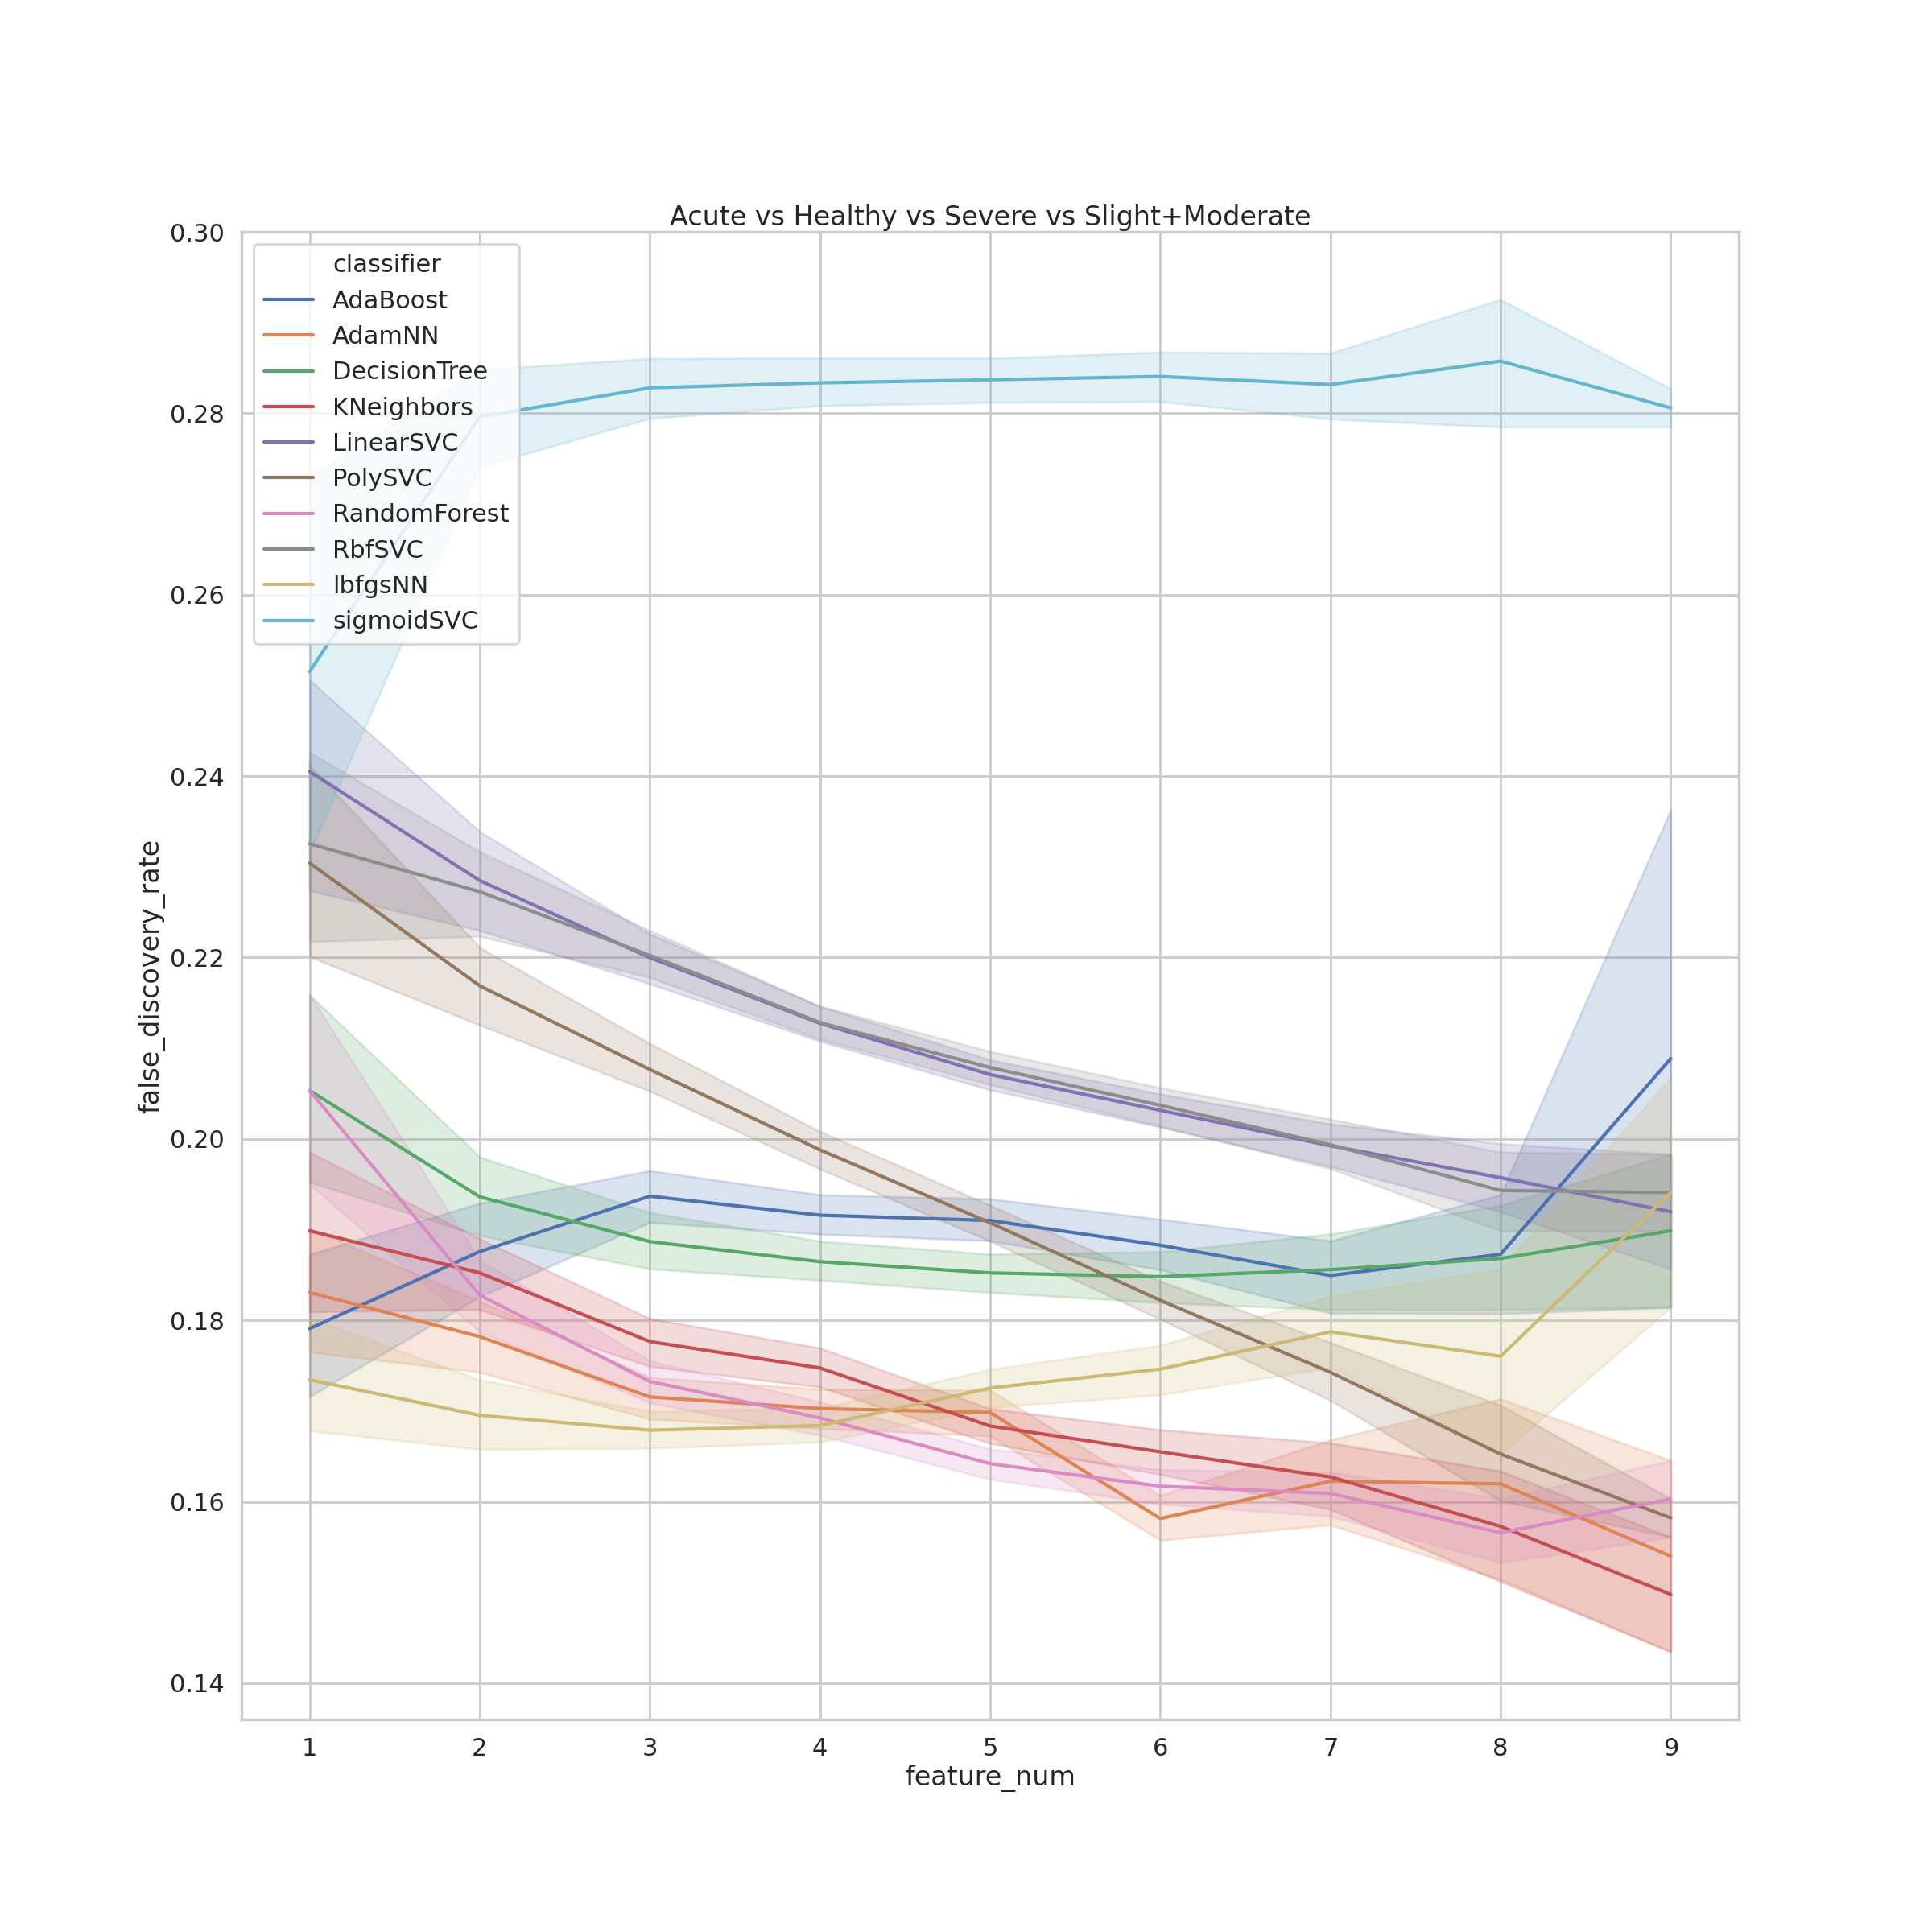
\includegraphics[width=0.3 \linewidth]{figures/Slight-Moderate/false_discovery_rate.png}
	    				&
	    				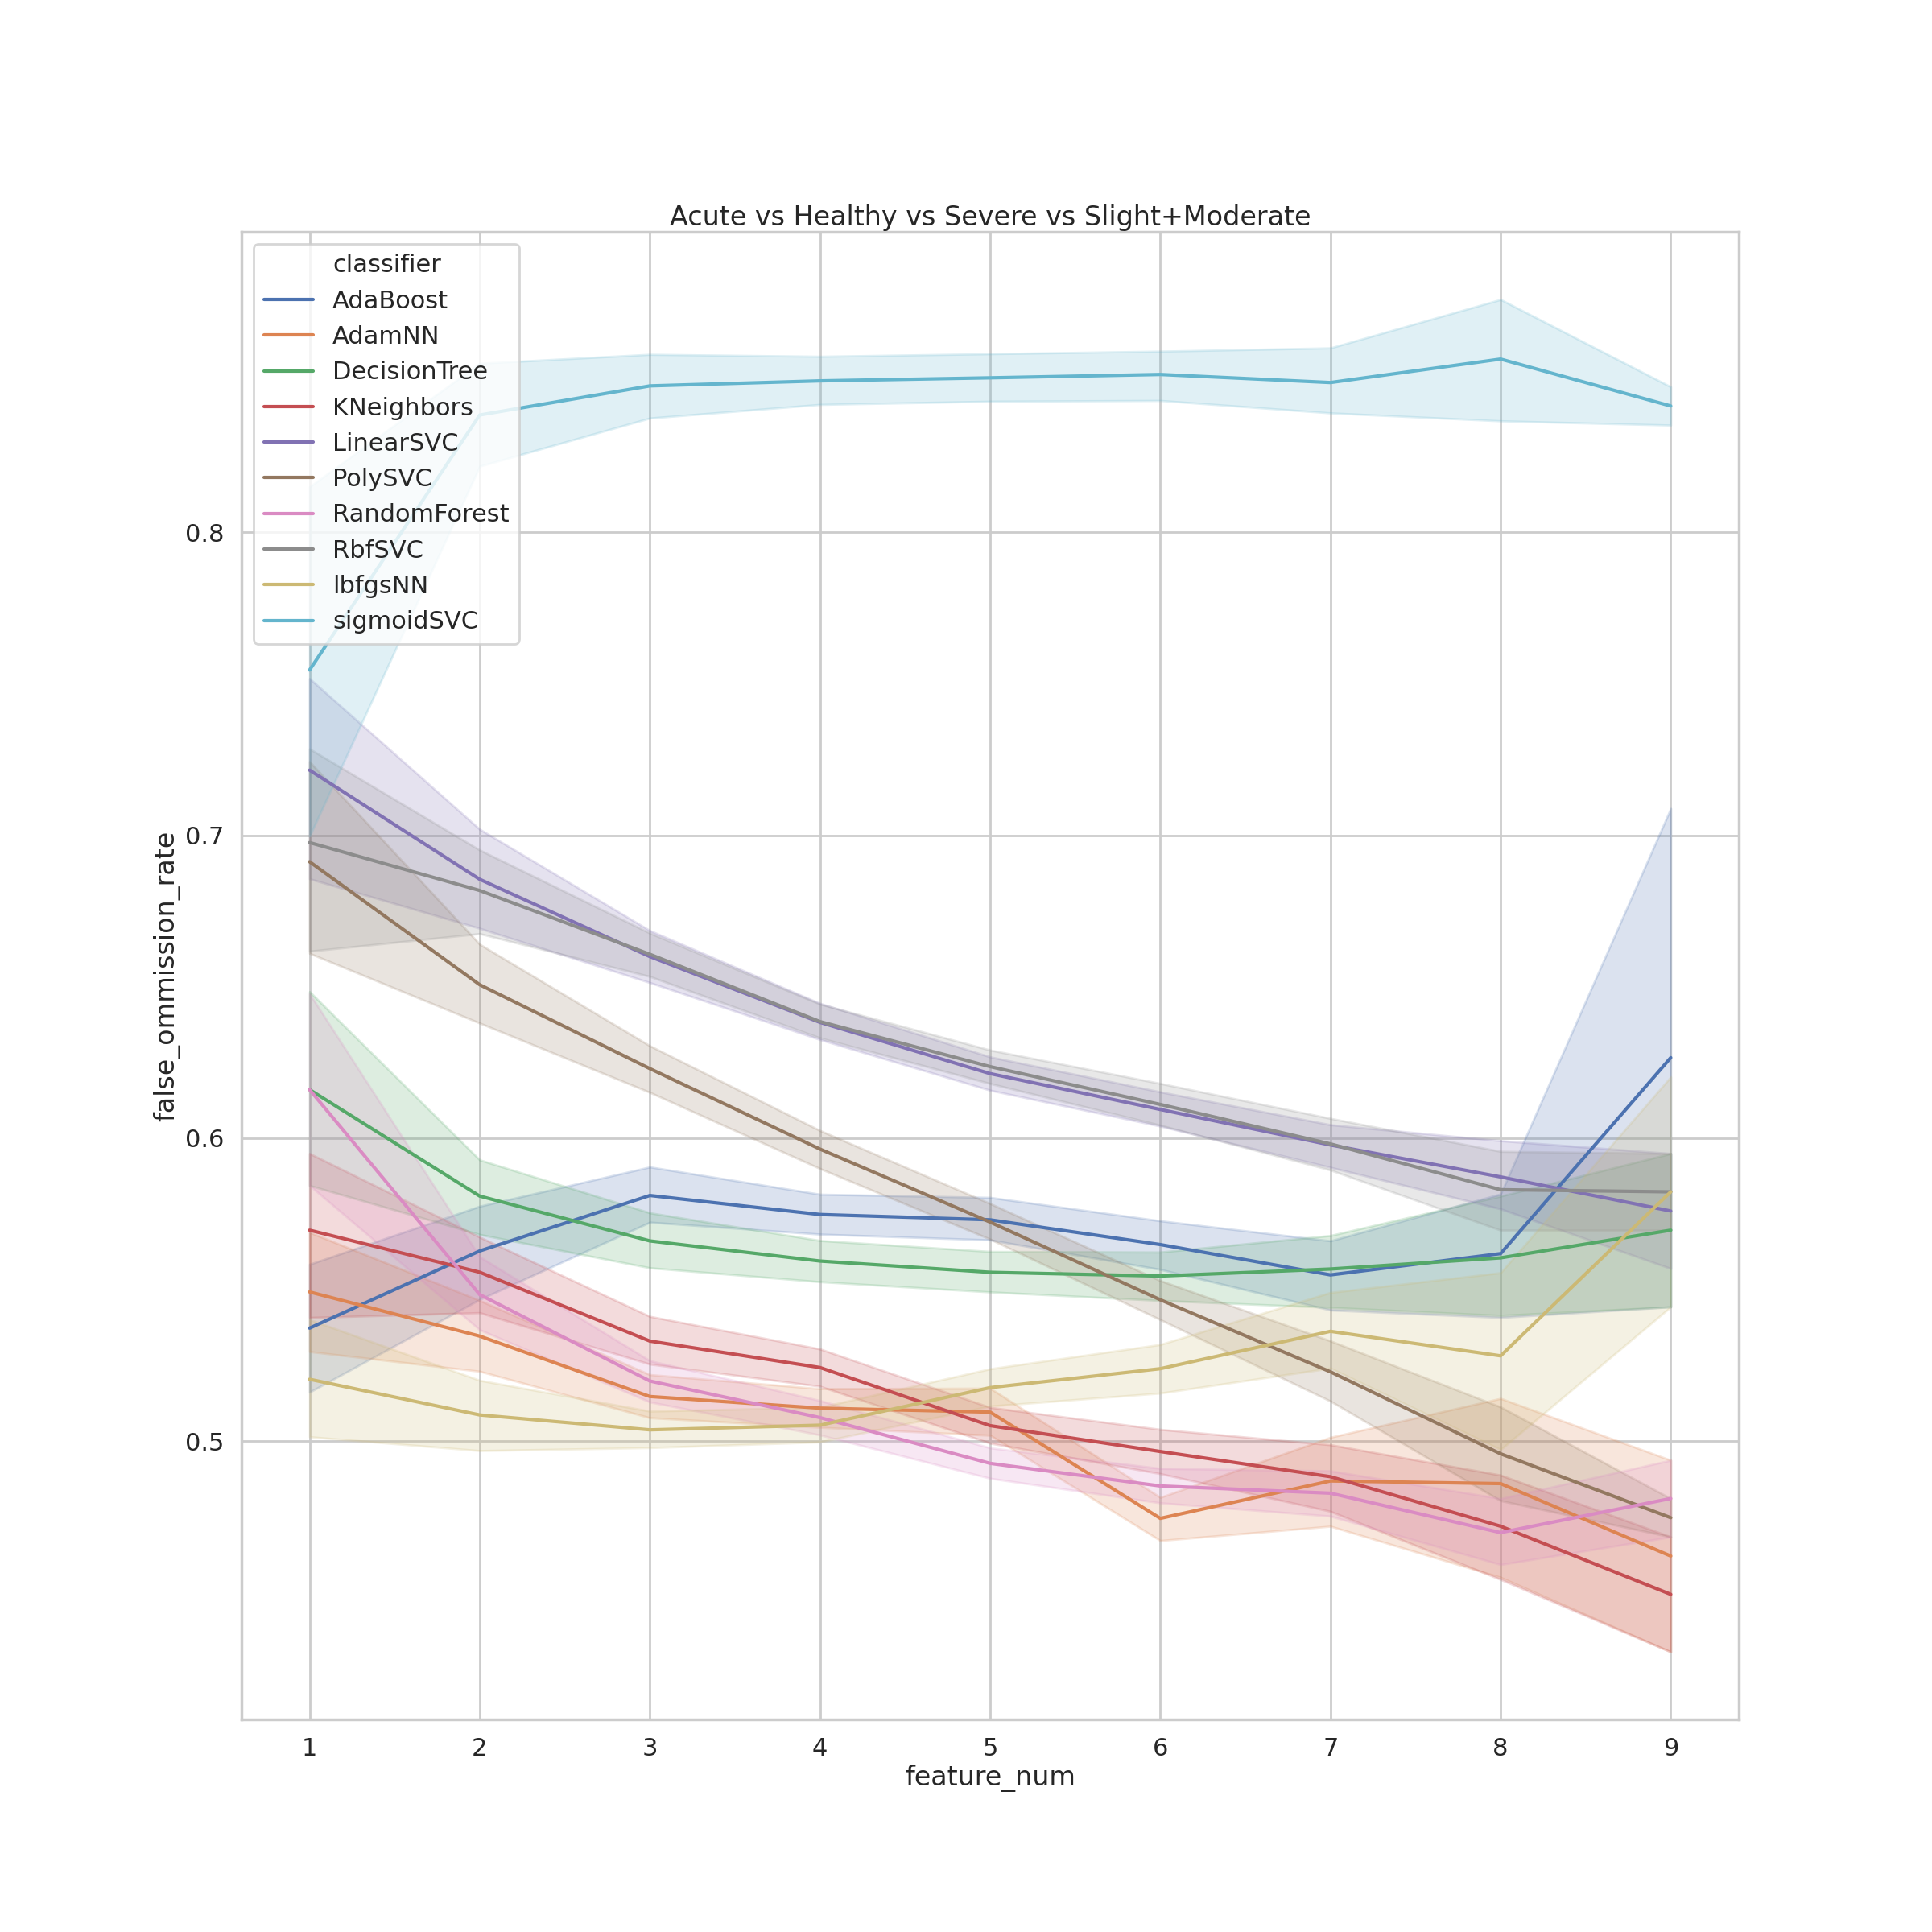
\includegraphics[width=0.3 \linewidth]{figures/Slight-Moderate/false_ommission_rate.png}
	    				&
	    				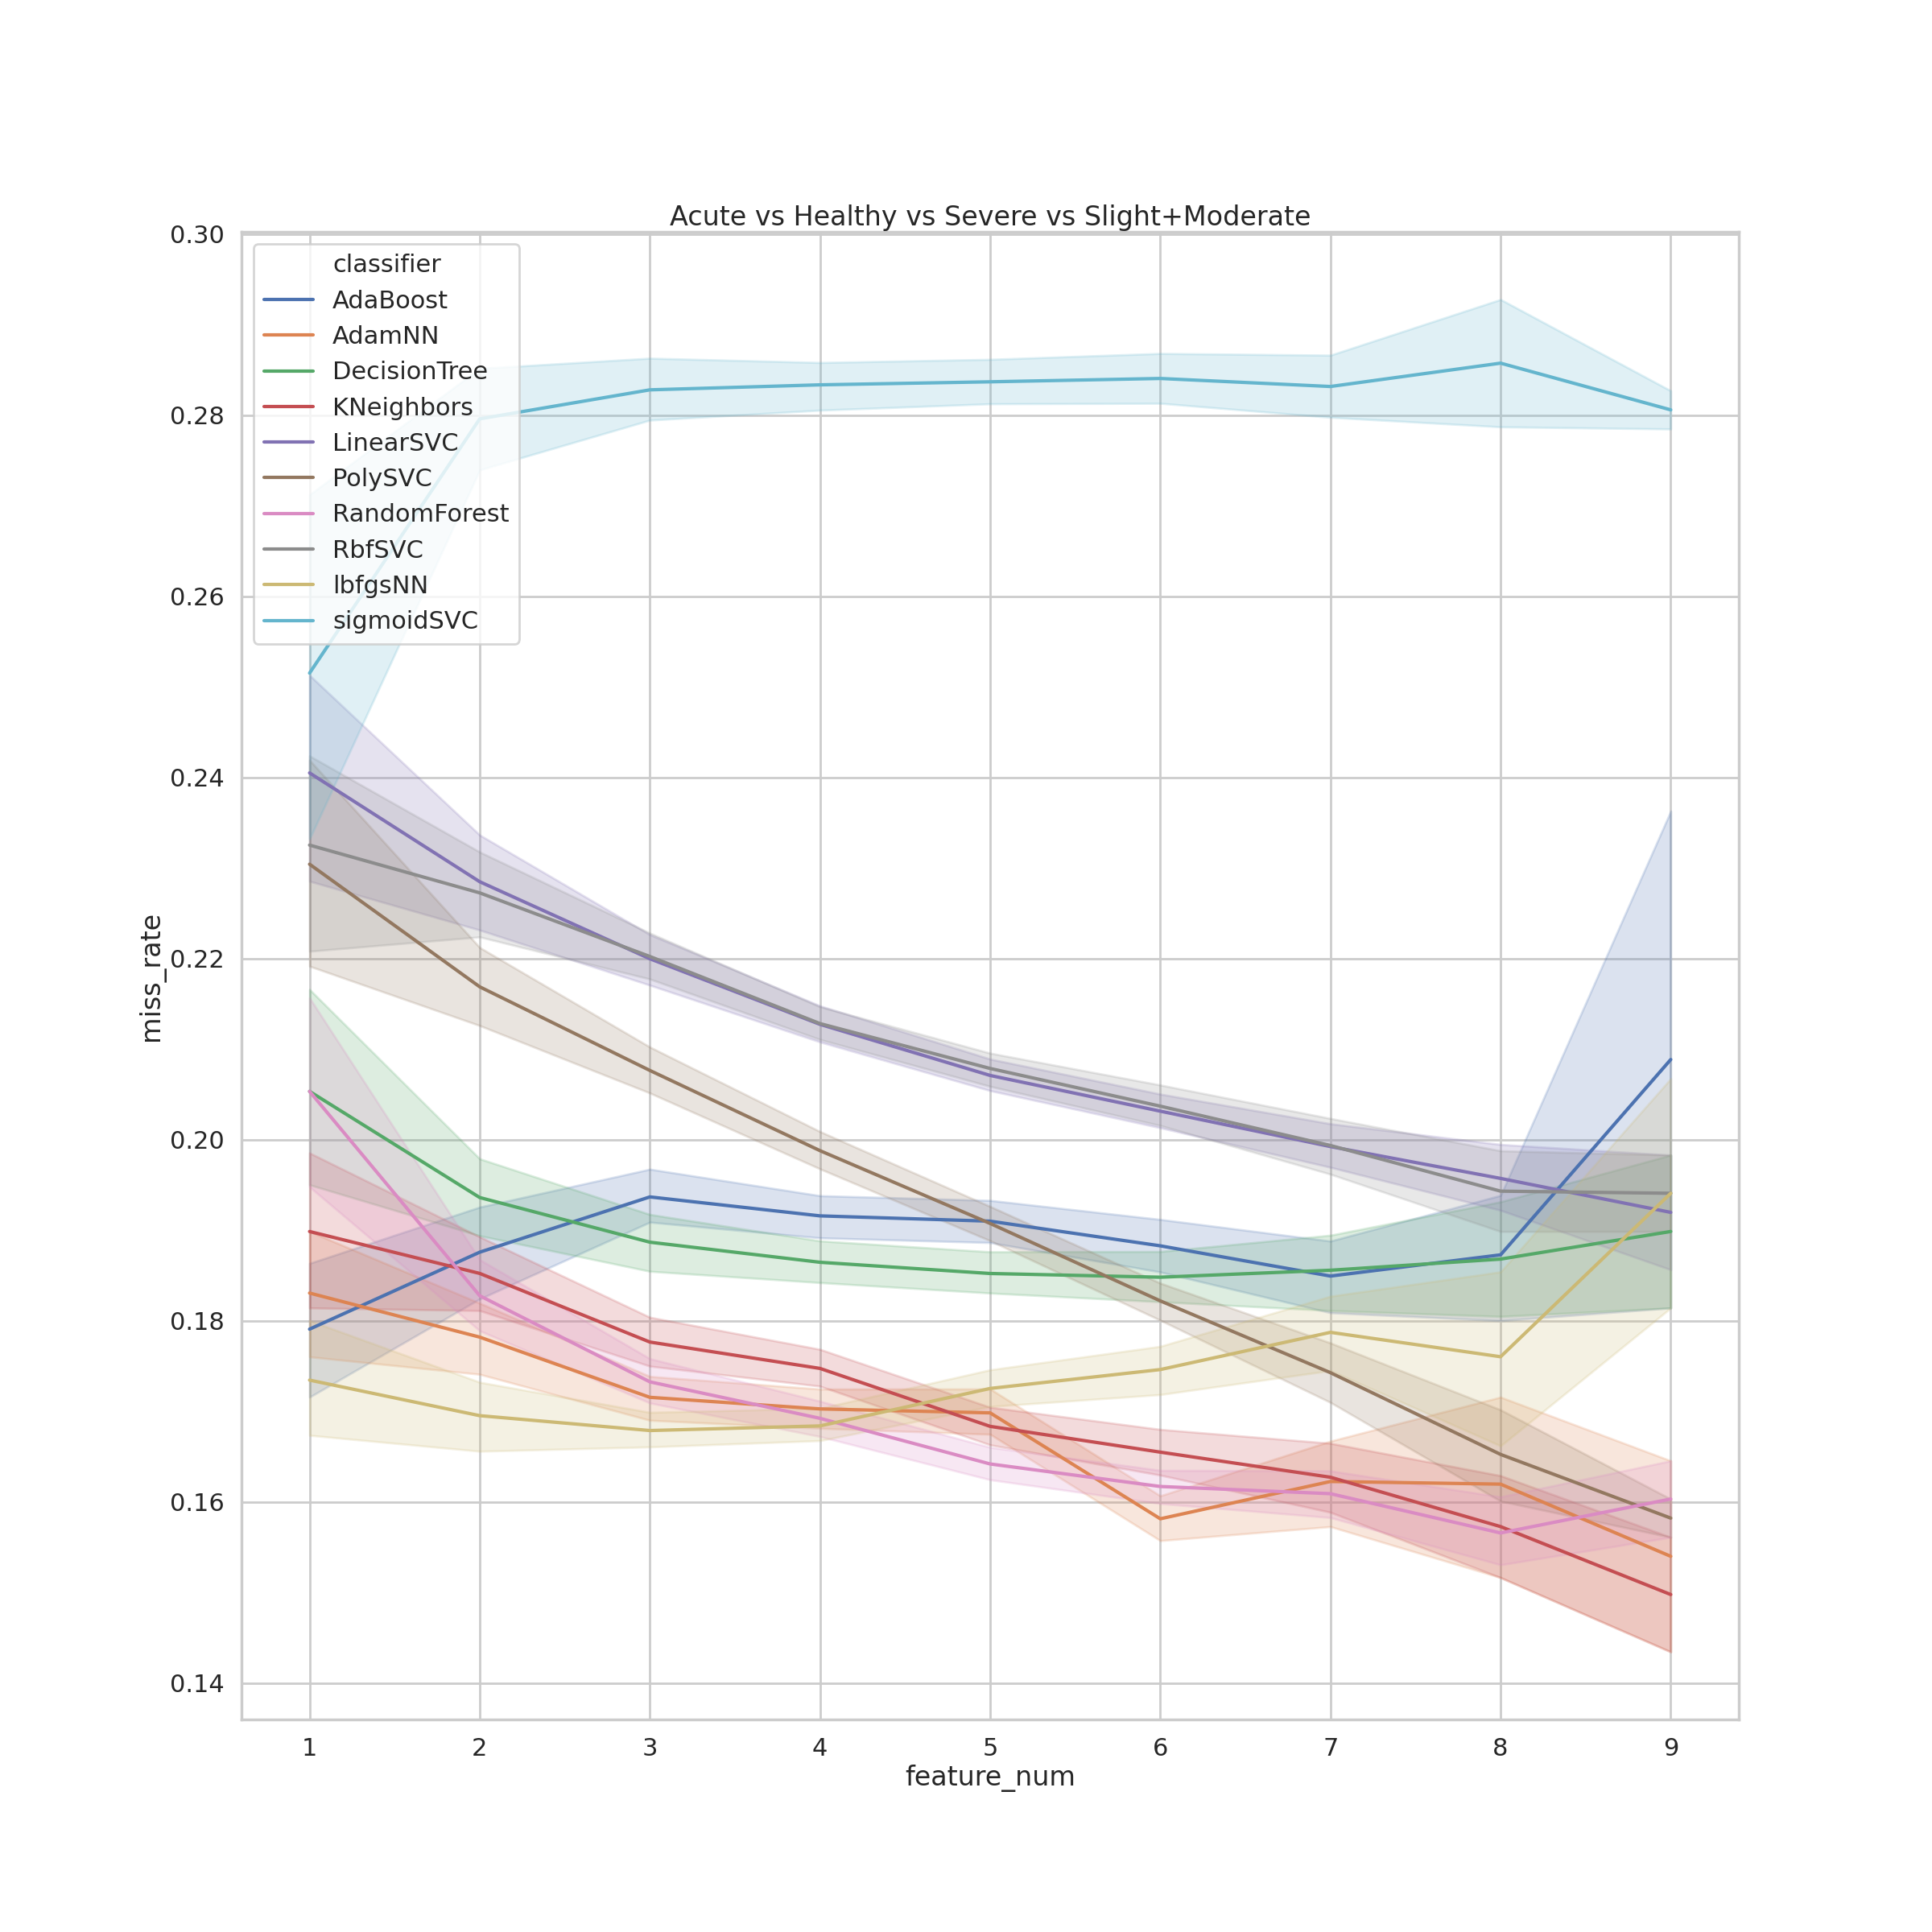
\includegraphics[width=0.3 \linewidth]{figures/Slight-Moderate/miss_rate.png}
	    				\\
	    				\mbox{False discovery rate} & \mbox{False ommision rate} & \mbox{Miss rate} \\ 
	    				
	    				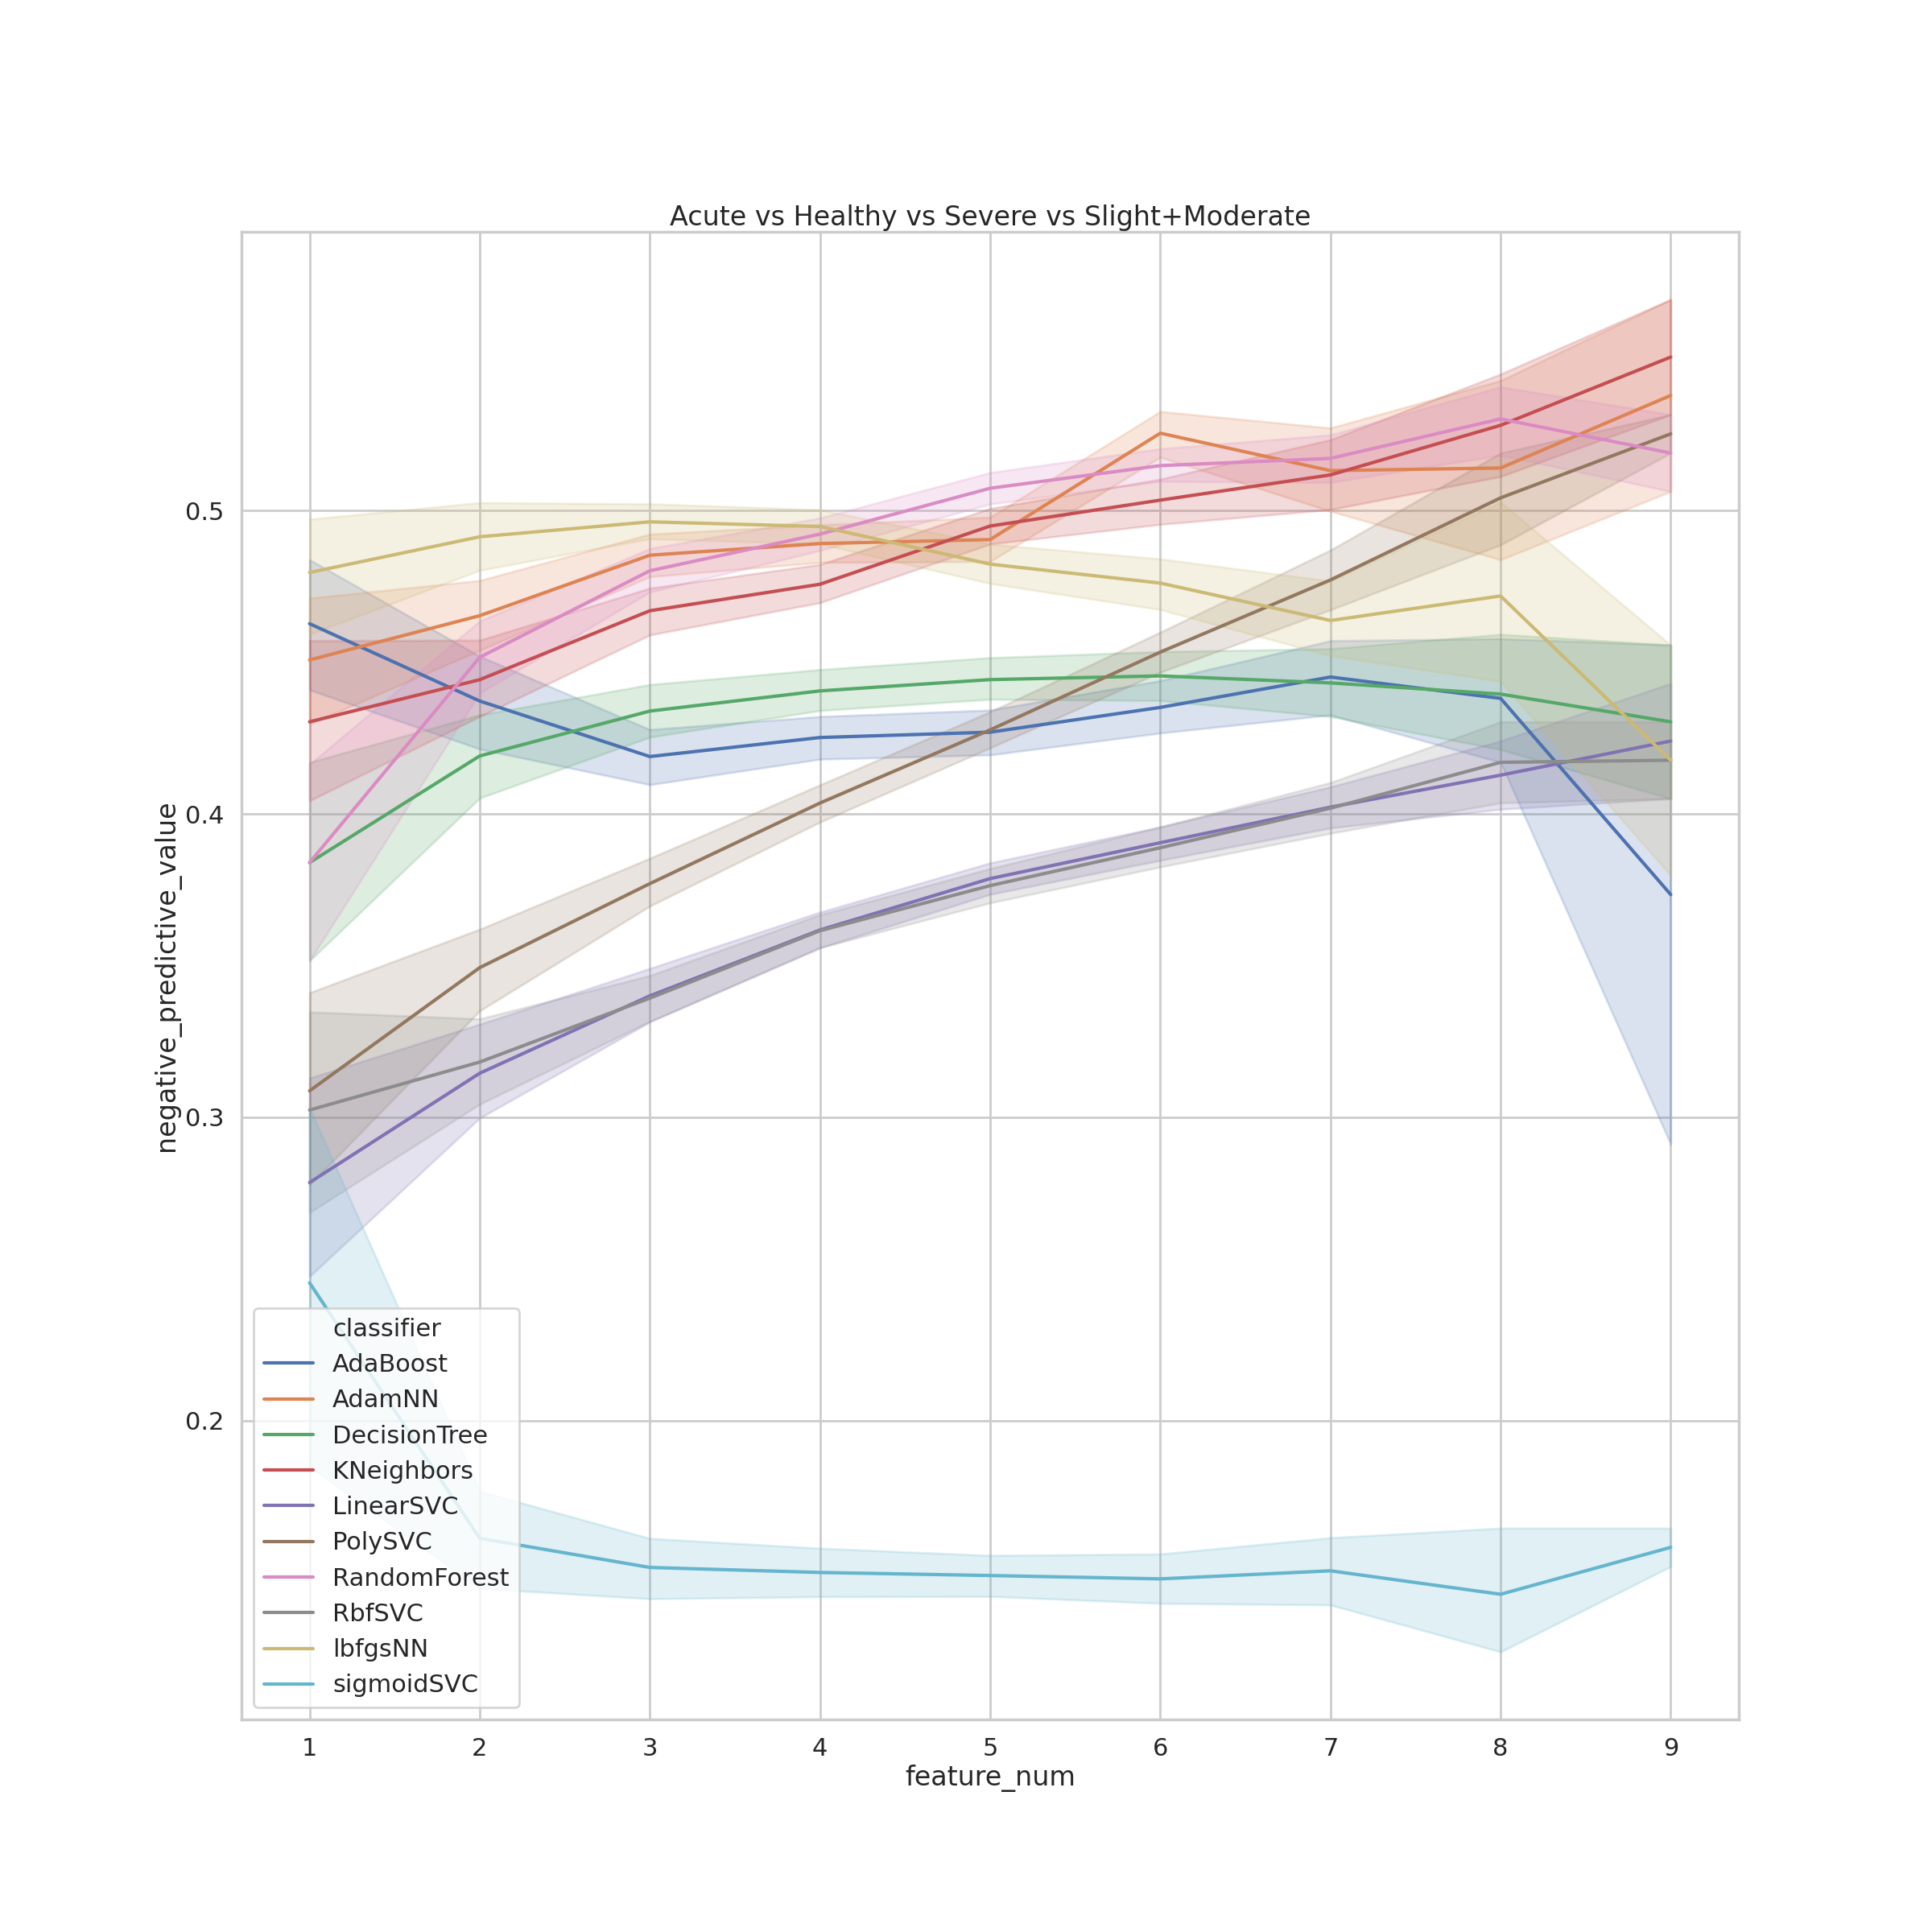
\includegraphics[width=0.3 \linewidth]{figures/Slight-Moderate/negative_predictive_value.png}
	    				&
	    				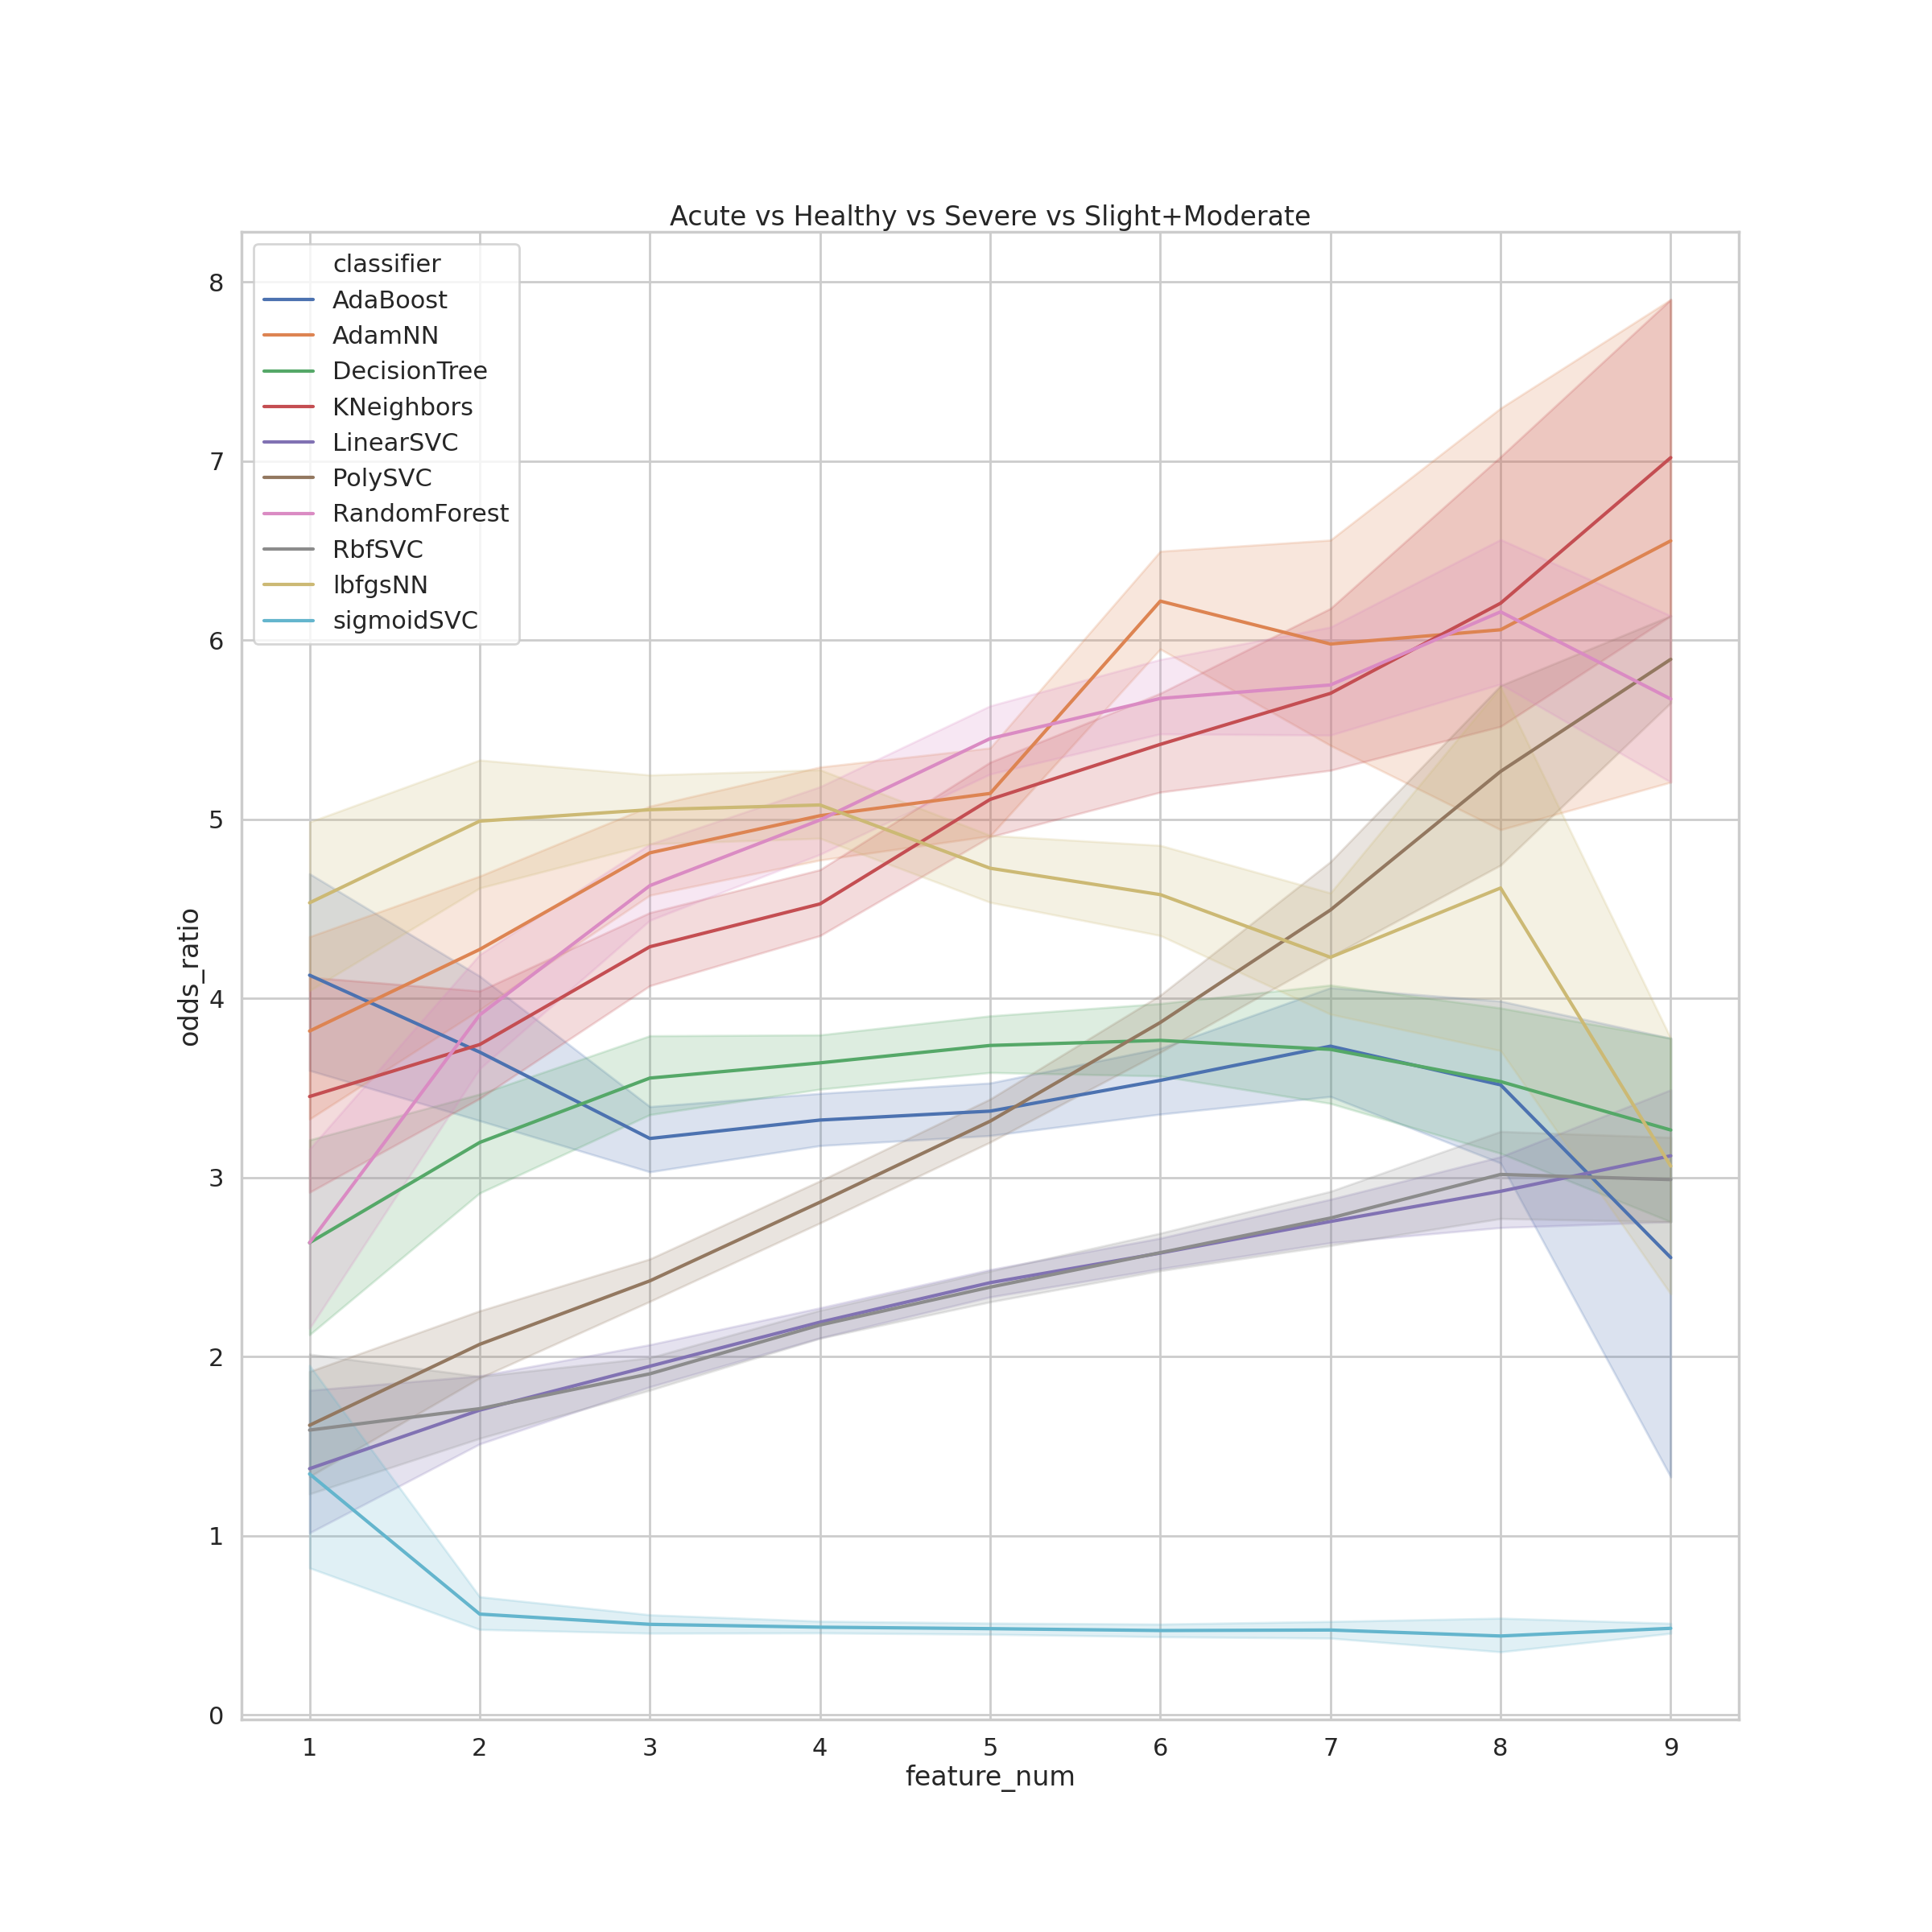
\includegraphics[width=0.3 \linewidth]{figures/Slight-Moderate/odds_ratio.png}
	    				&
	    				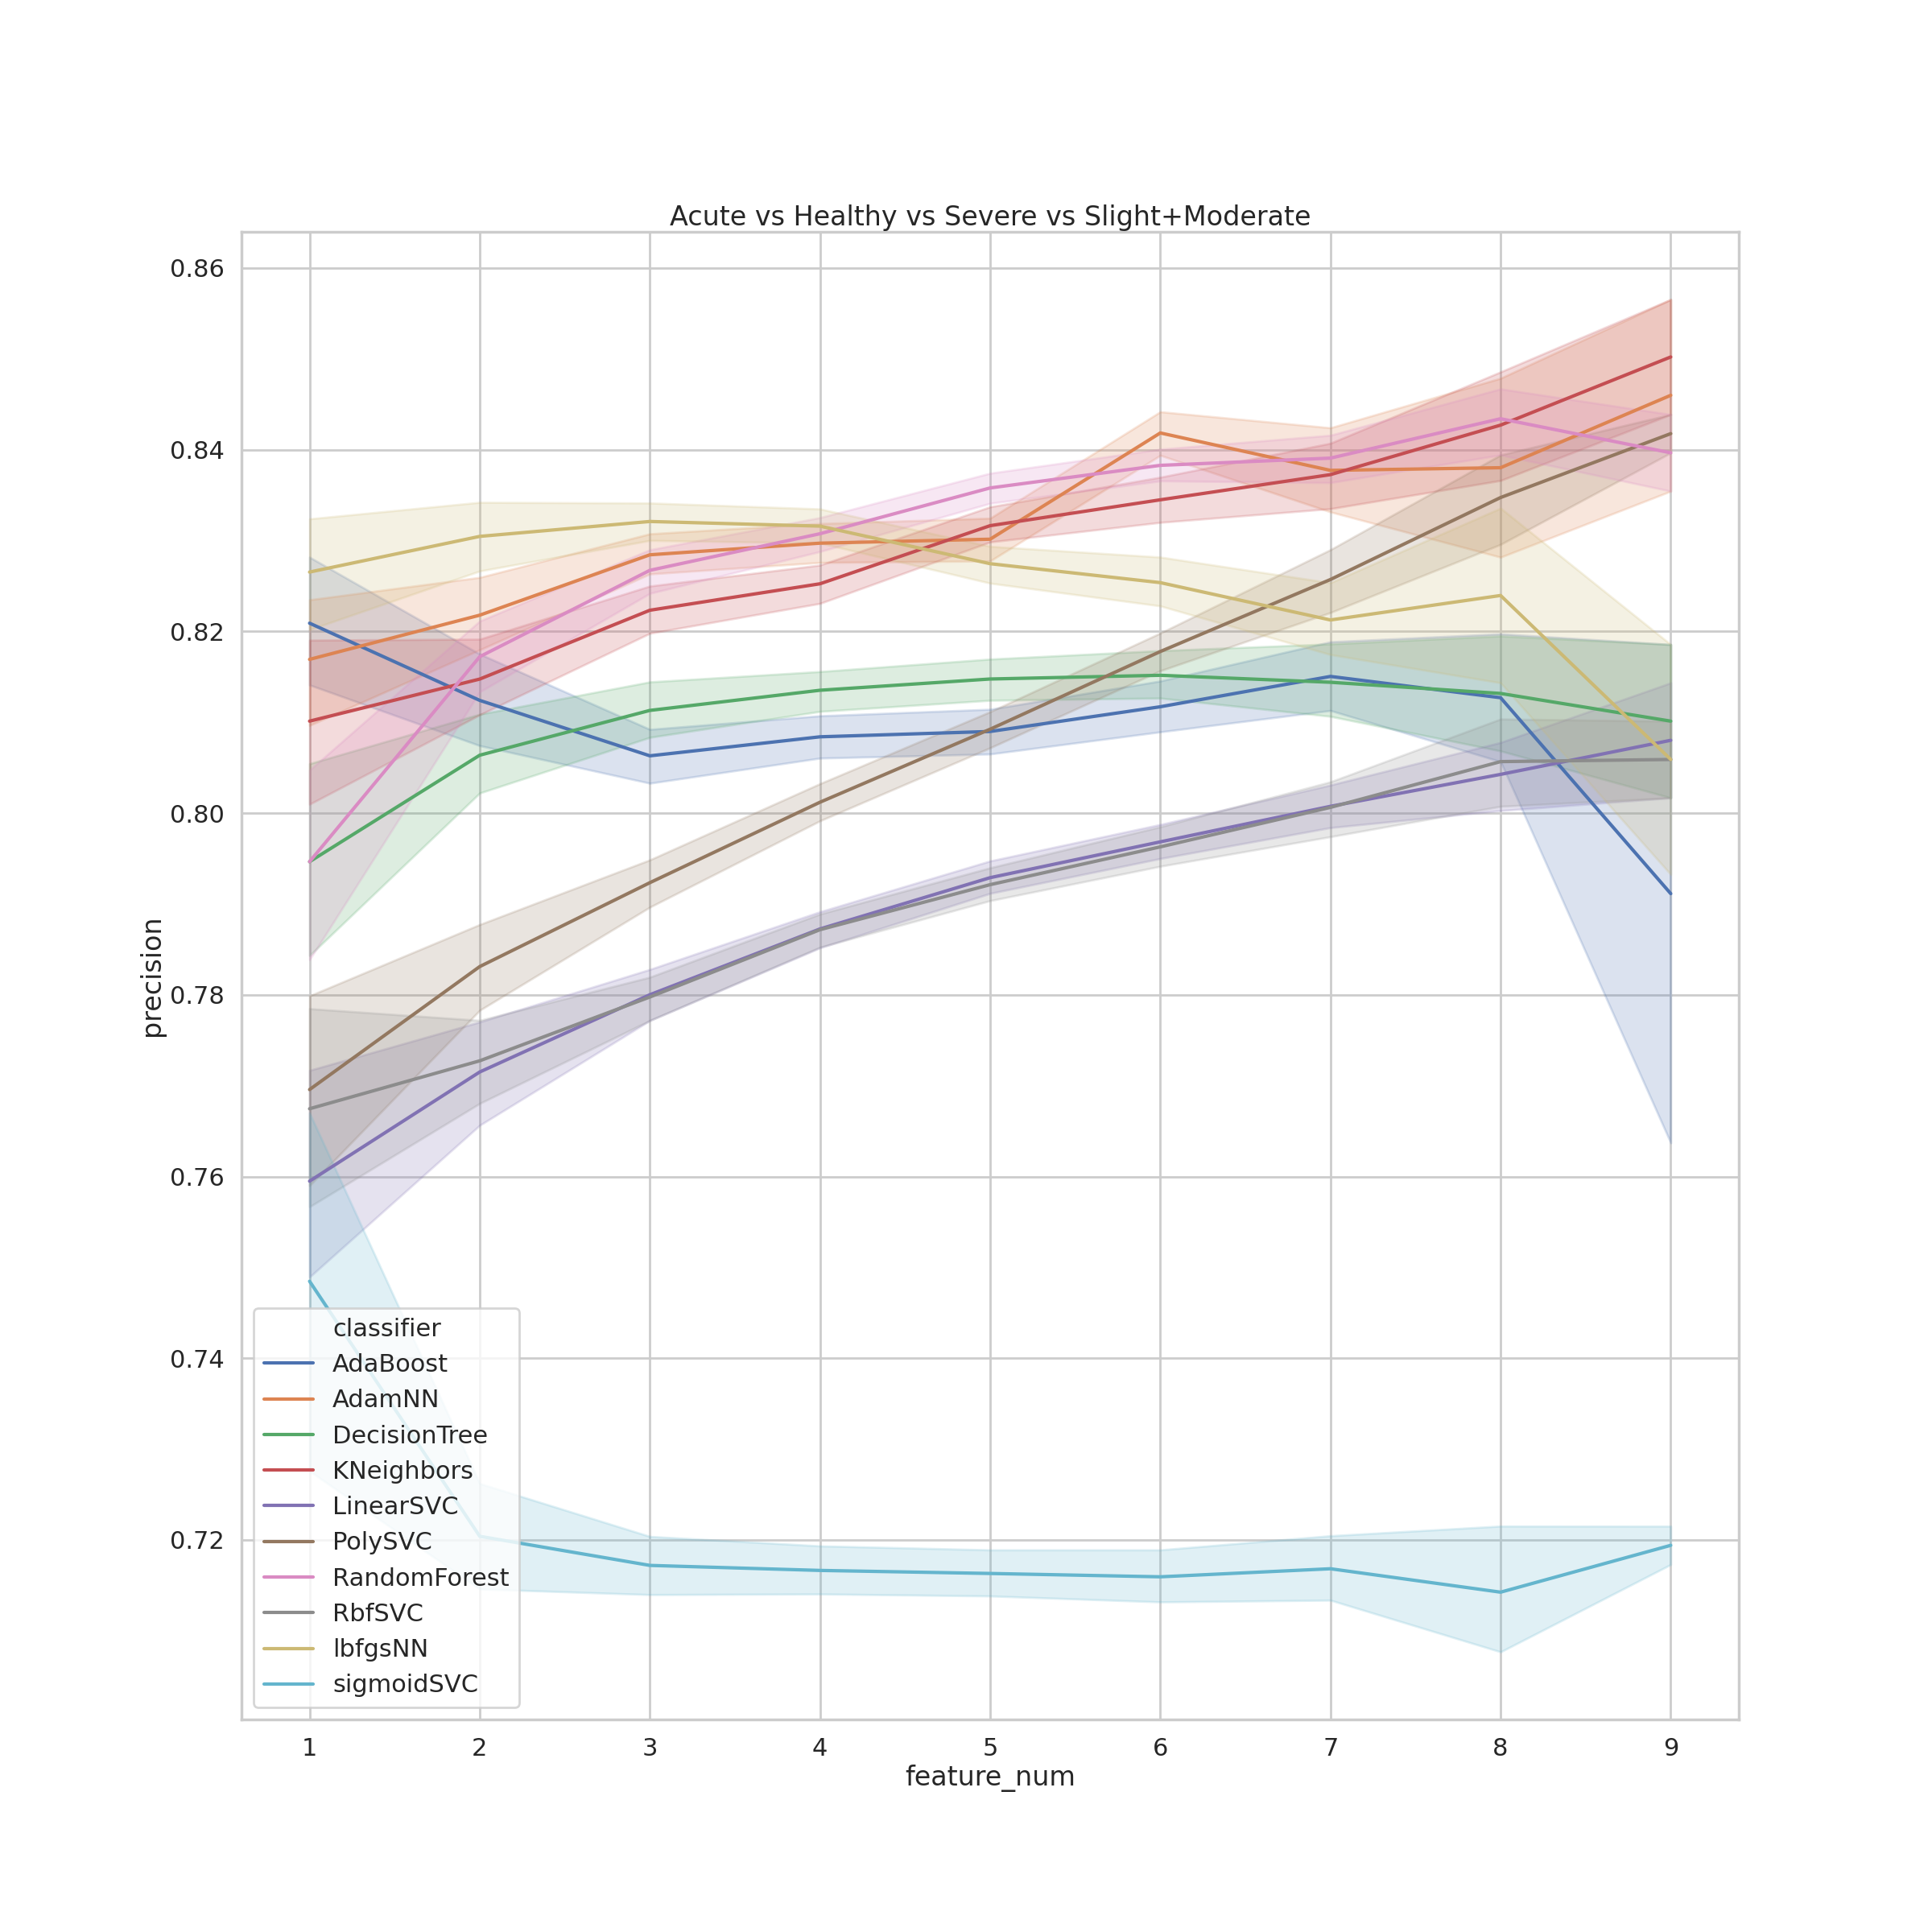
\includegraphics[width=0.3 \linewidth]{figures/Slight-Moderate/precision.png}
	    				\\
	    				\mbox{Negative predictive value} & \mbox{Odds ratio} & \mbox{Precision} \\ 
	    				
	    				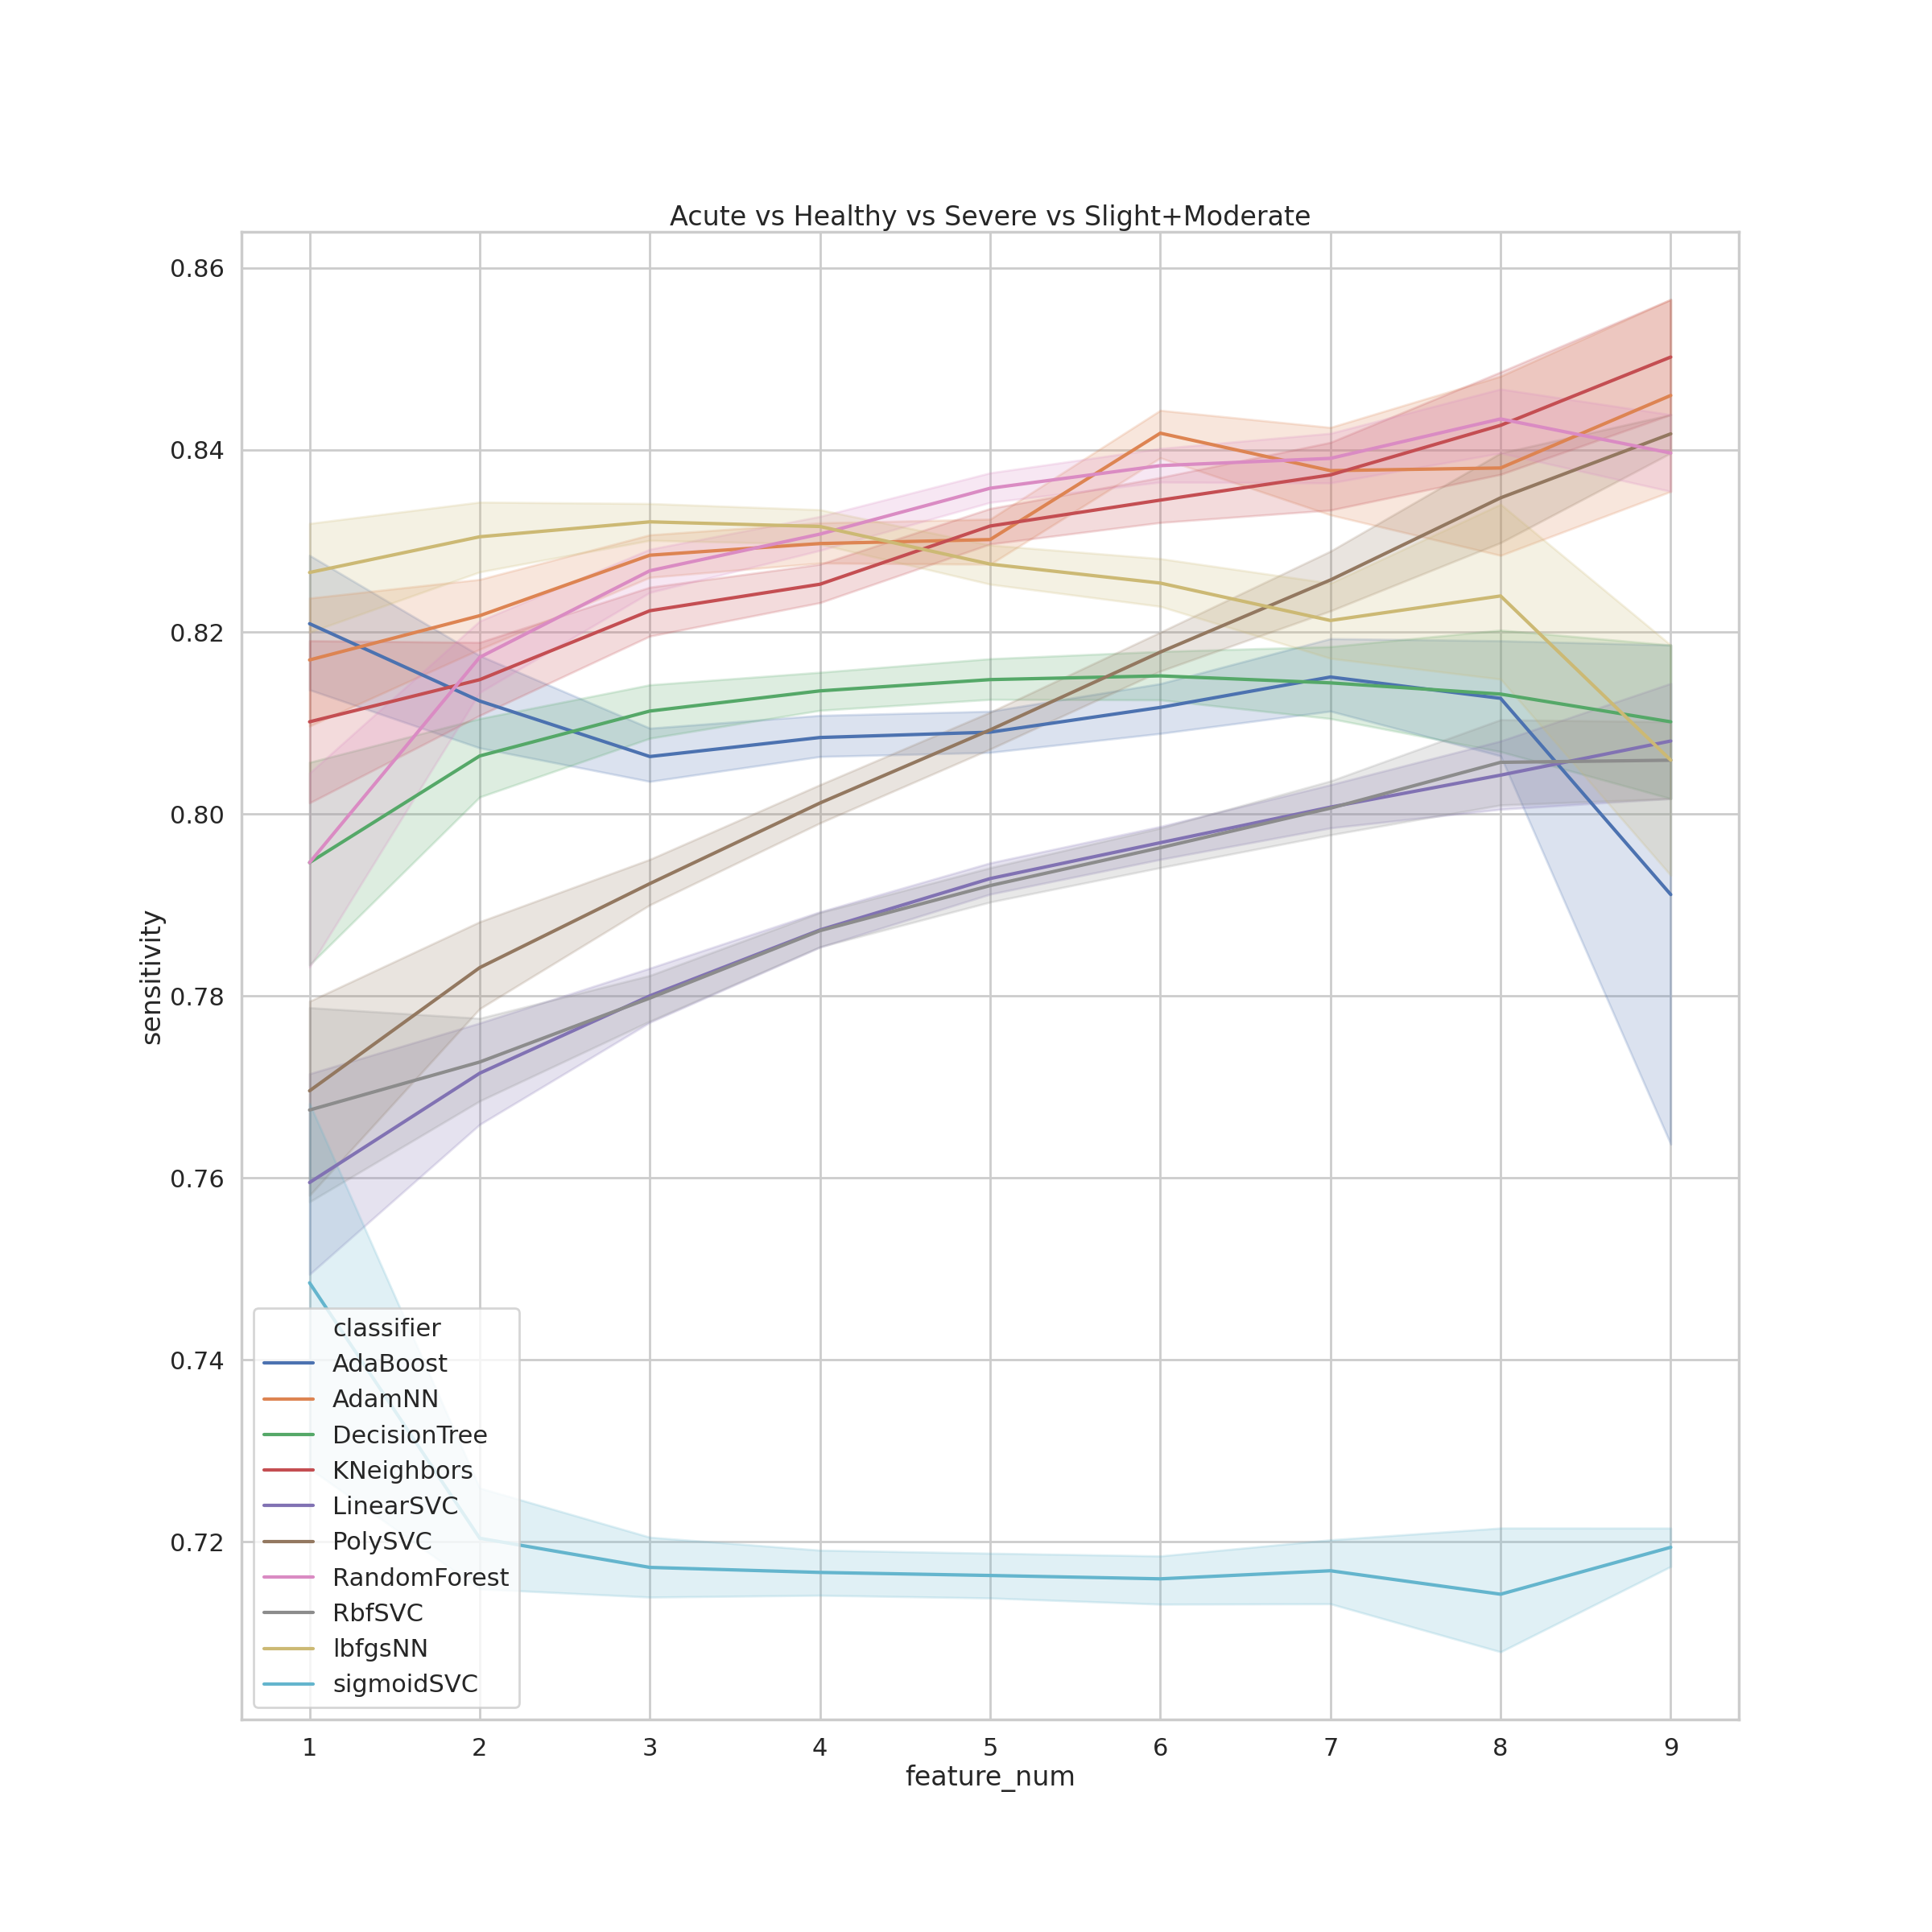
\includegraphics[width=0.3 \linewidth]{figures/Slight-Moderate/sensitivity.png}
	    				&
	    				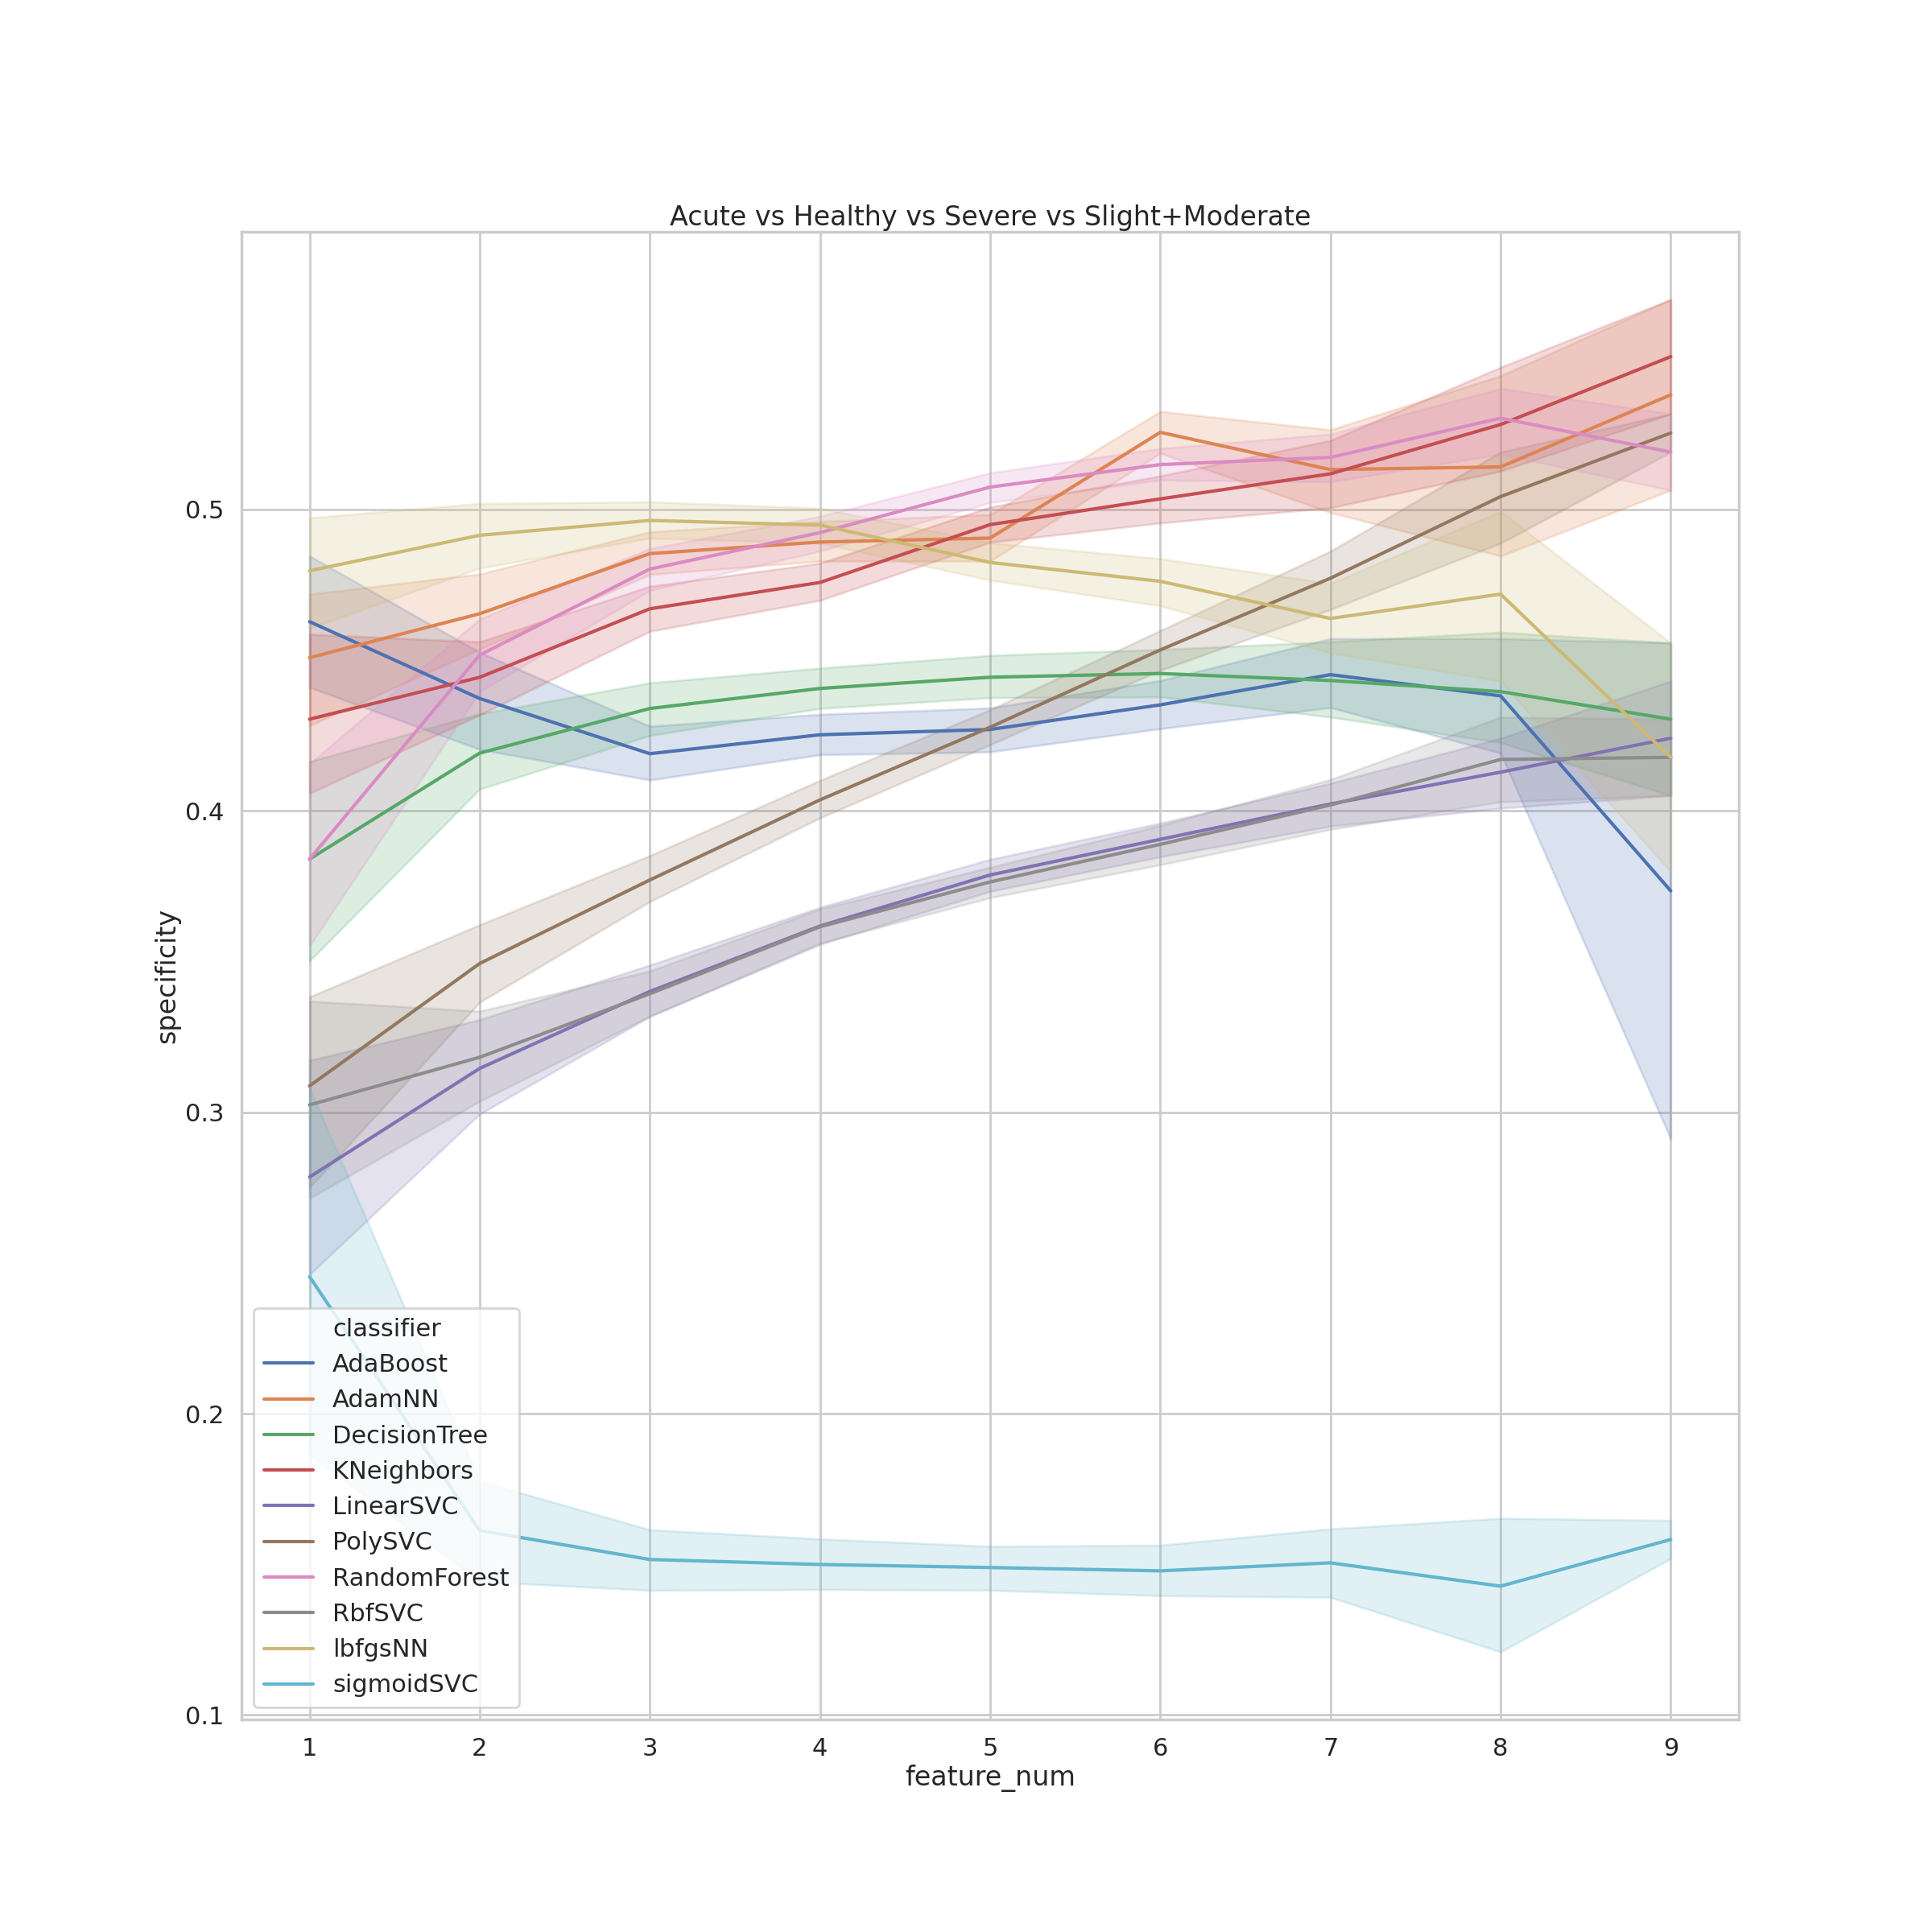
\includegraphics[width=0.3 \linewidth]{figures/Slight-Moderate/specificity.png}
	    				&
	    				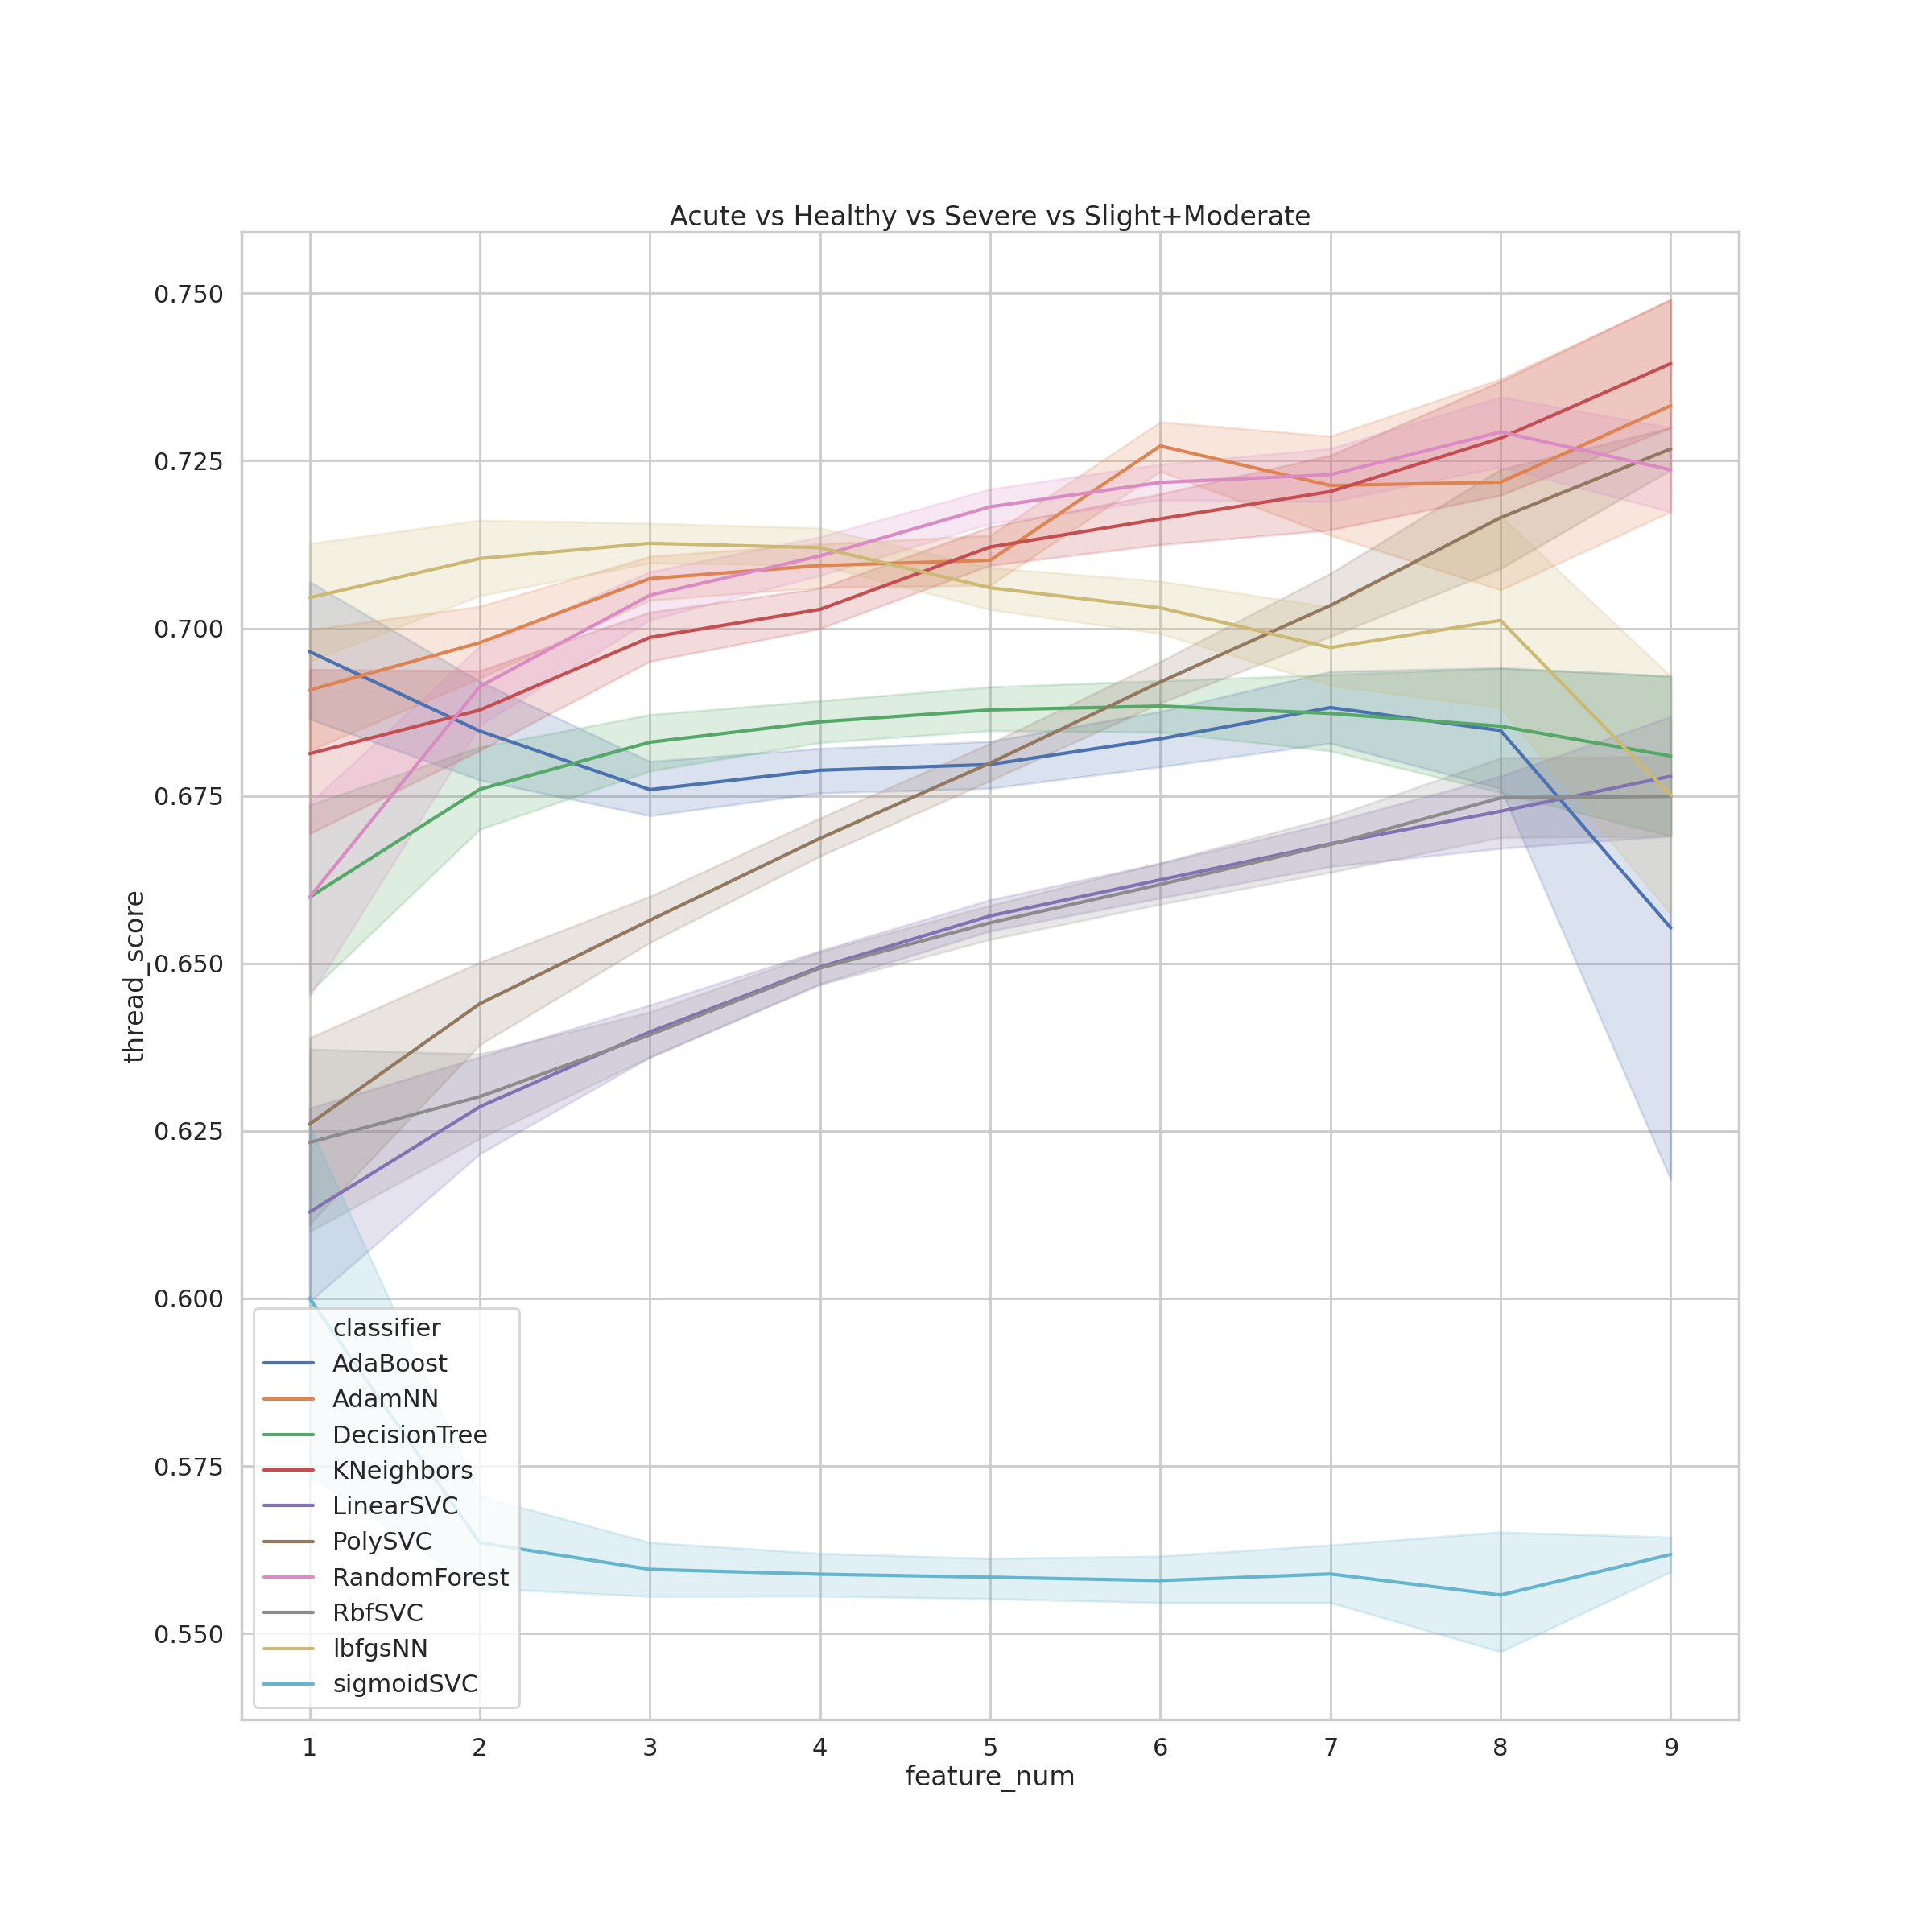
\includegraphics[width=0.3 \linewidth]{figures/Slight-Moderate/thread_score.png}
	    				\\
	    				\mbox{Sensitivity} & \mbox{Specificity} & \mbox{Thread score} \\
	    			\end{array}$
	    			\caption{Confusion Matrix Derivations from Slight-Moderate Classification}
	    			\label{fig:sli-m-confusion}
    			\end{figure}
    		
				\begin{figure}[htbp]
					\centering
					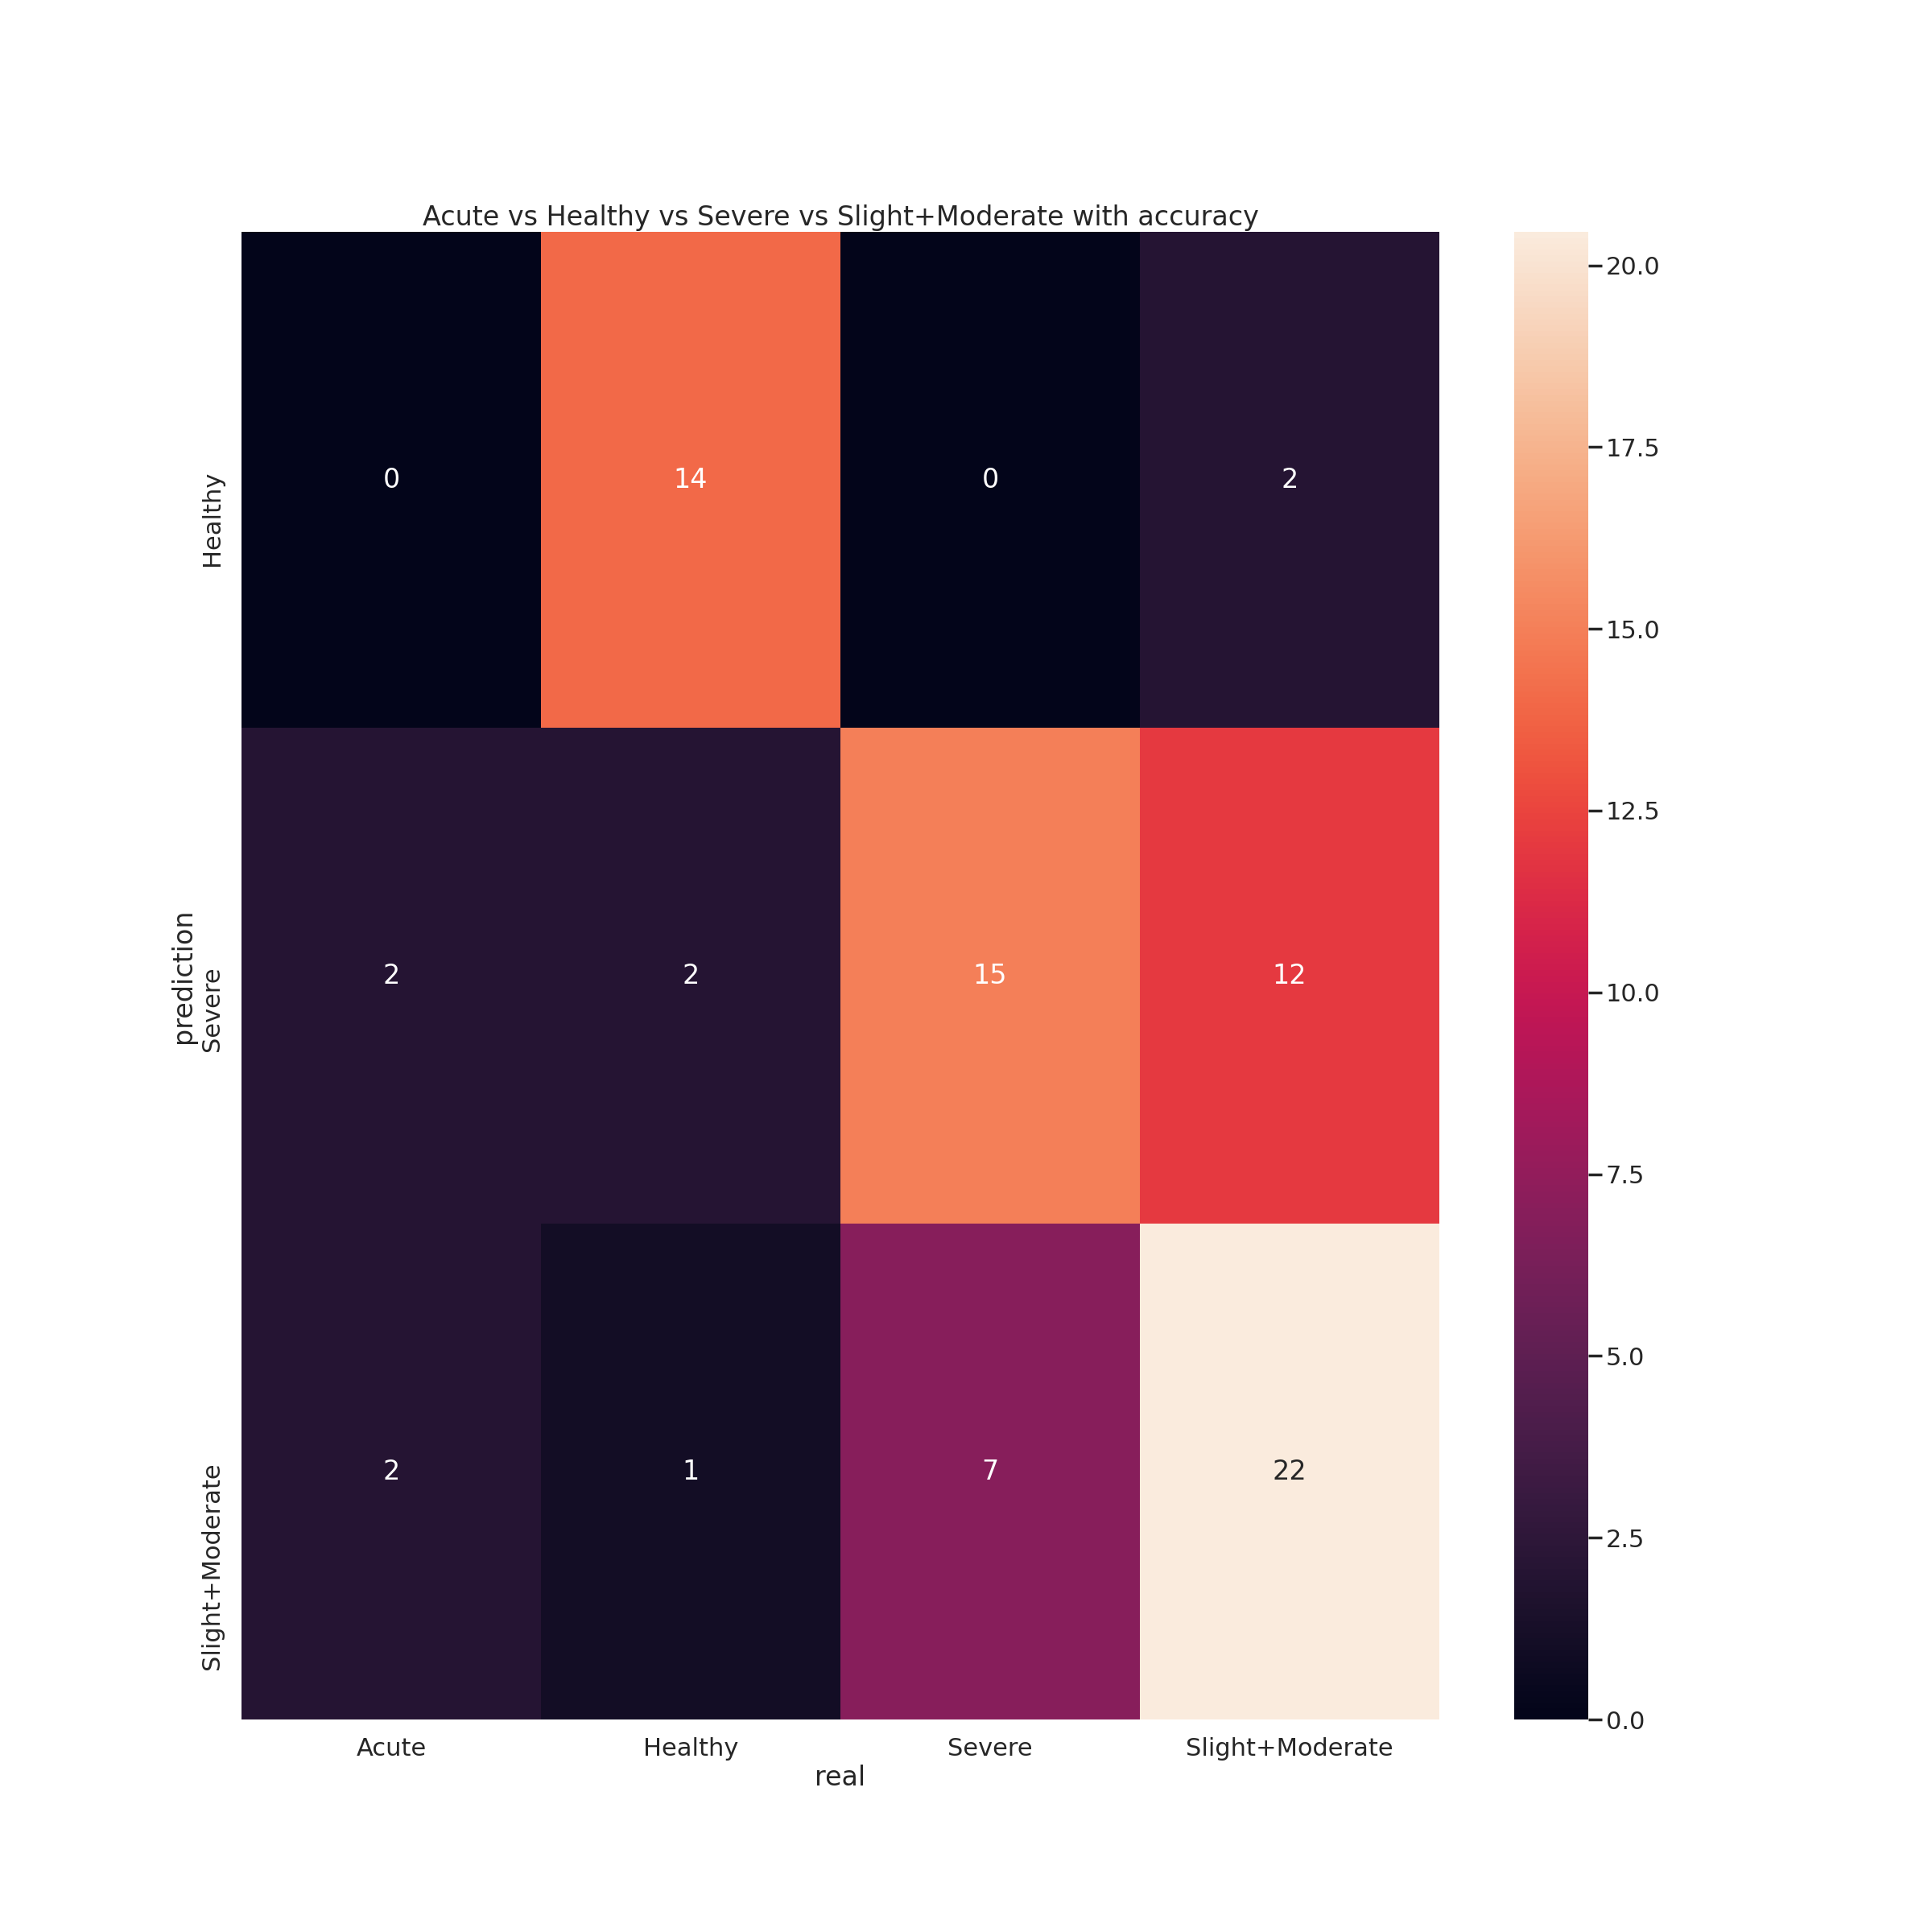
\includegraphics[width=0.5 \linewidth]{figures/Slight-Moderate/heatmap.png}
					\caption{Heatmap Plot for Merged Slight-Moderate Classification with Random Forest}
					\label{fig:sli-m-heatmap}
				\end{figure}
    		
    		\subsubsection{Merged Moderate-Severe Class}
    			Figure \ref{fig:m-s-confusion} displays the derivations of confusion matrix in merged moderate-severe classification. Note that the values in figure \ref{fig:m-s-confusion}, mean values from combination which used same number of features will be shown. As figure \ref{fig:m-s-confusion}, the Random Forest algorithm has the best values with all features.
    		
    			\begin{figure}[htbp]
    				\centering
    				$\begin{array}{ccc}
	    				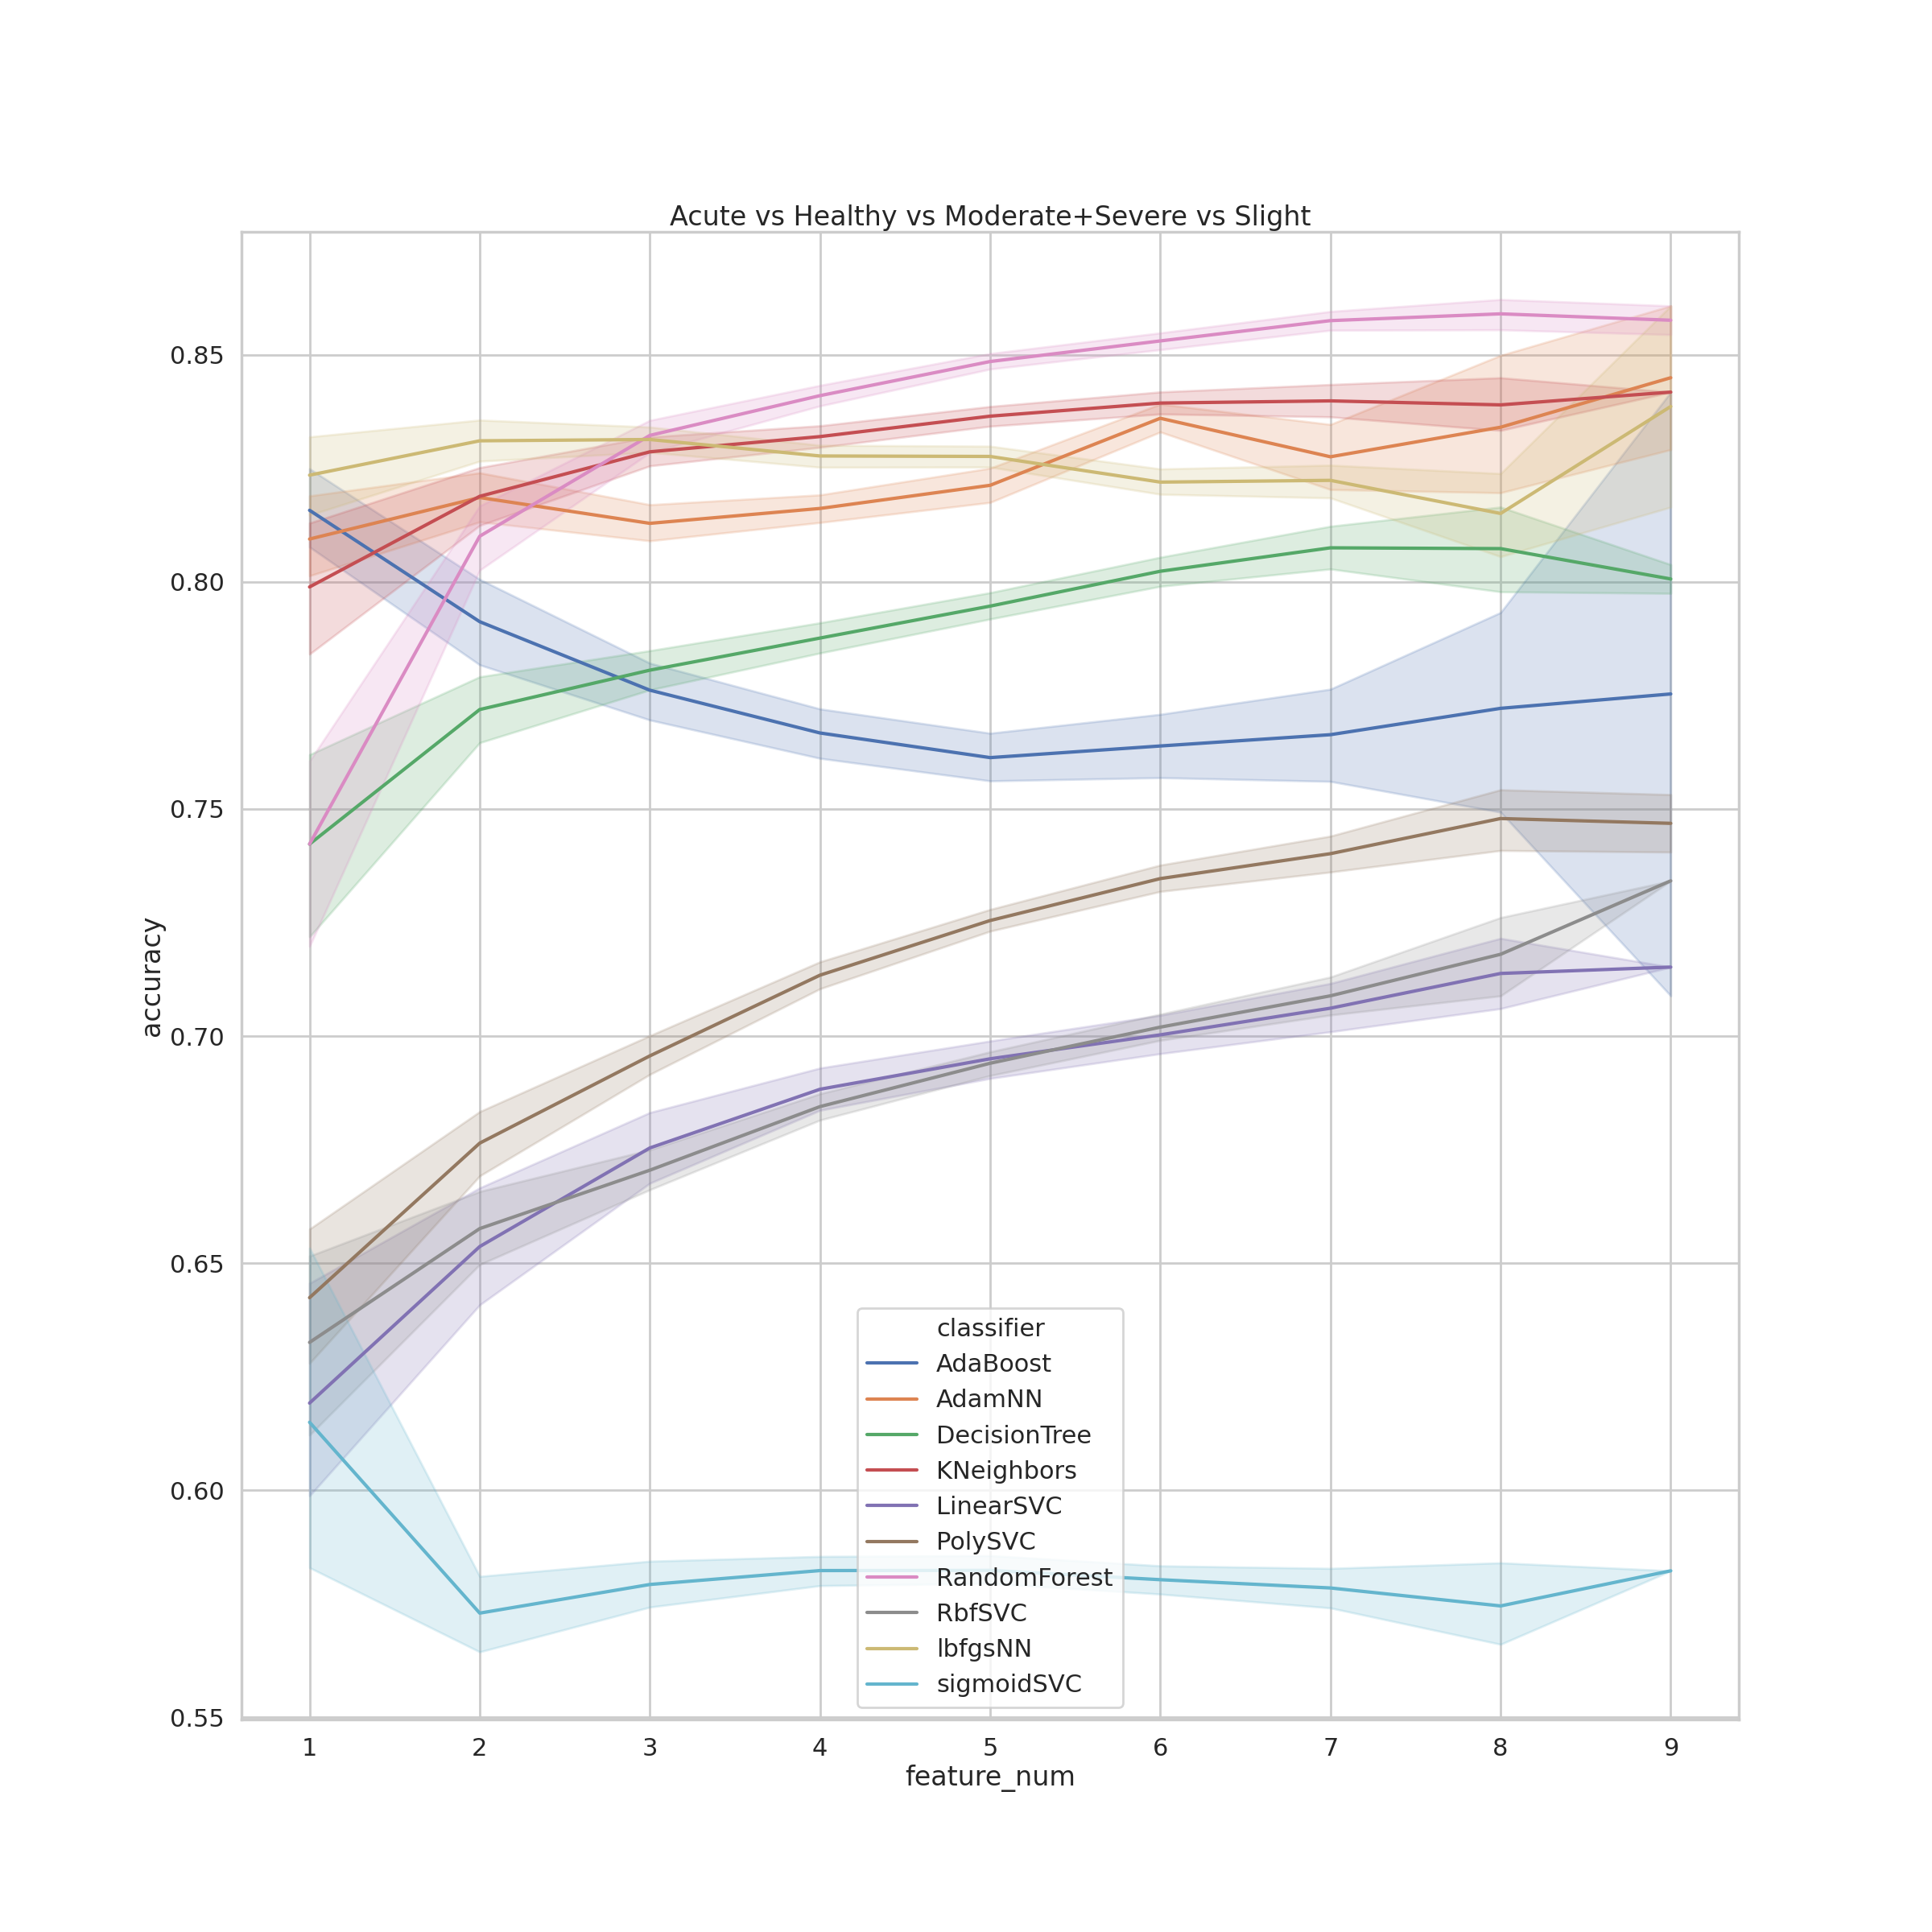
\includegraphics[width=0.3 \linewidth]{figures/Moderate-Severe/accuracy.png}
	    				&
	    				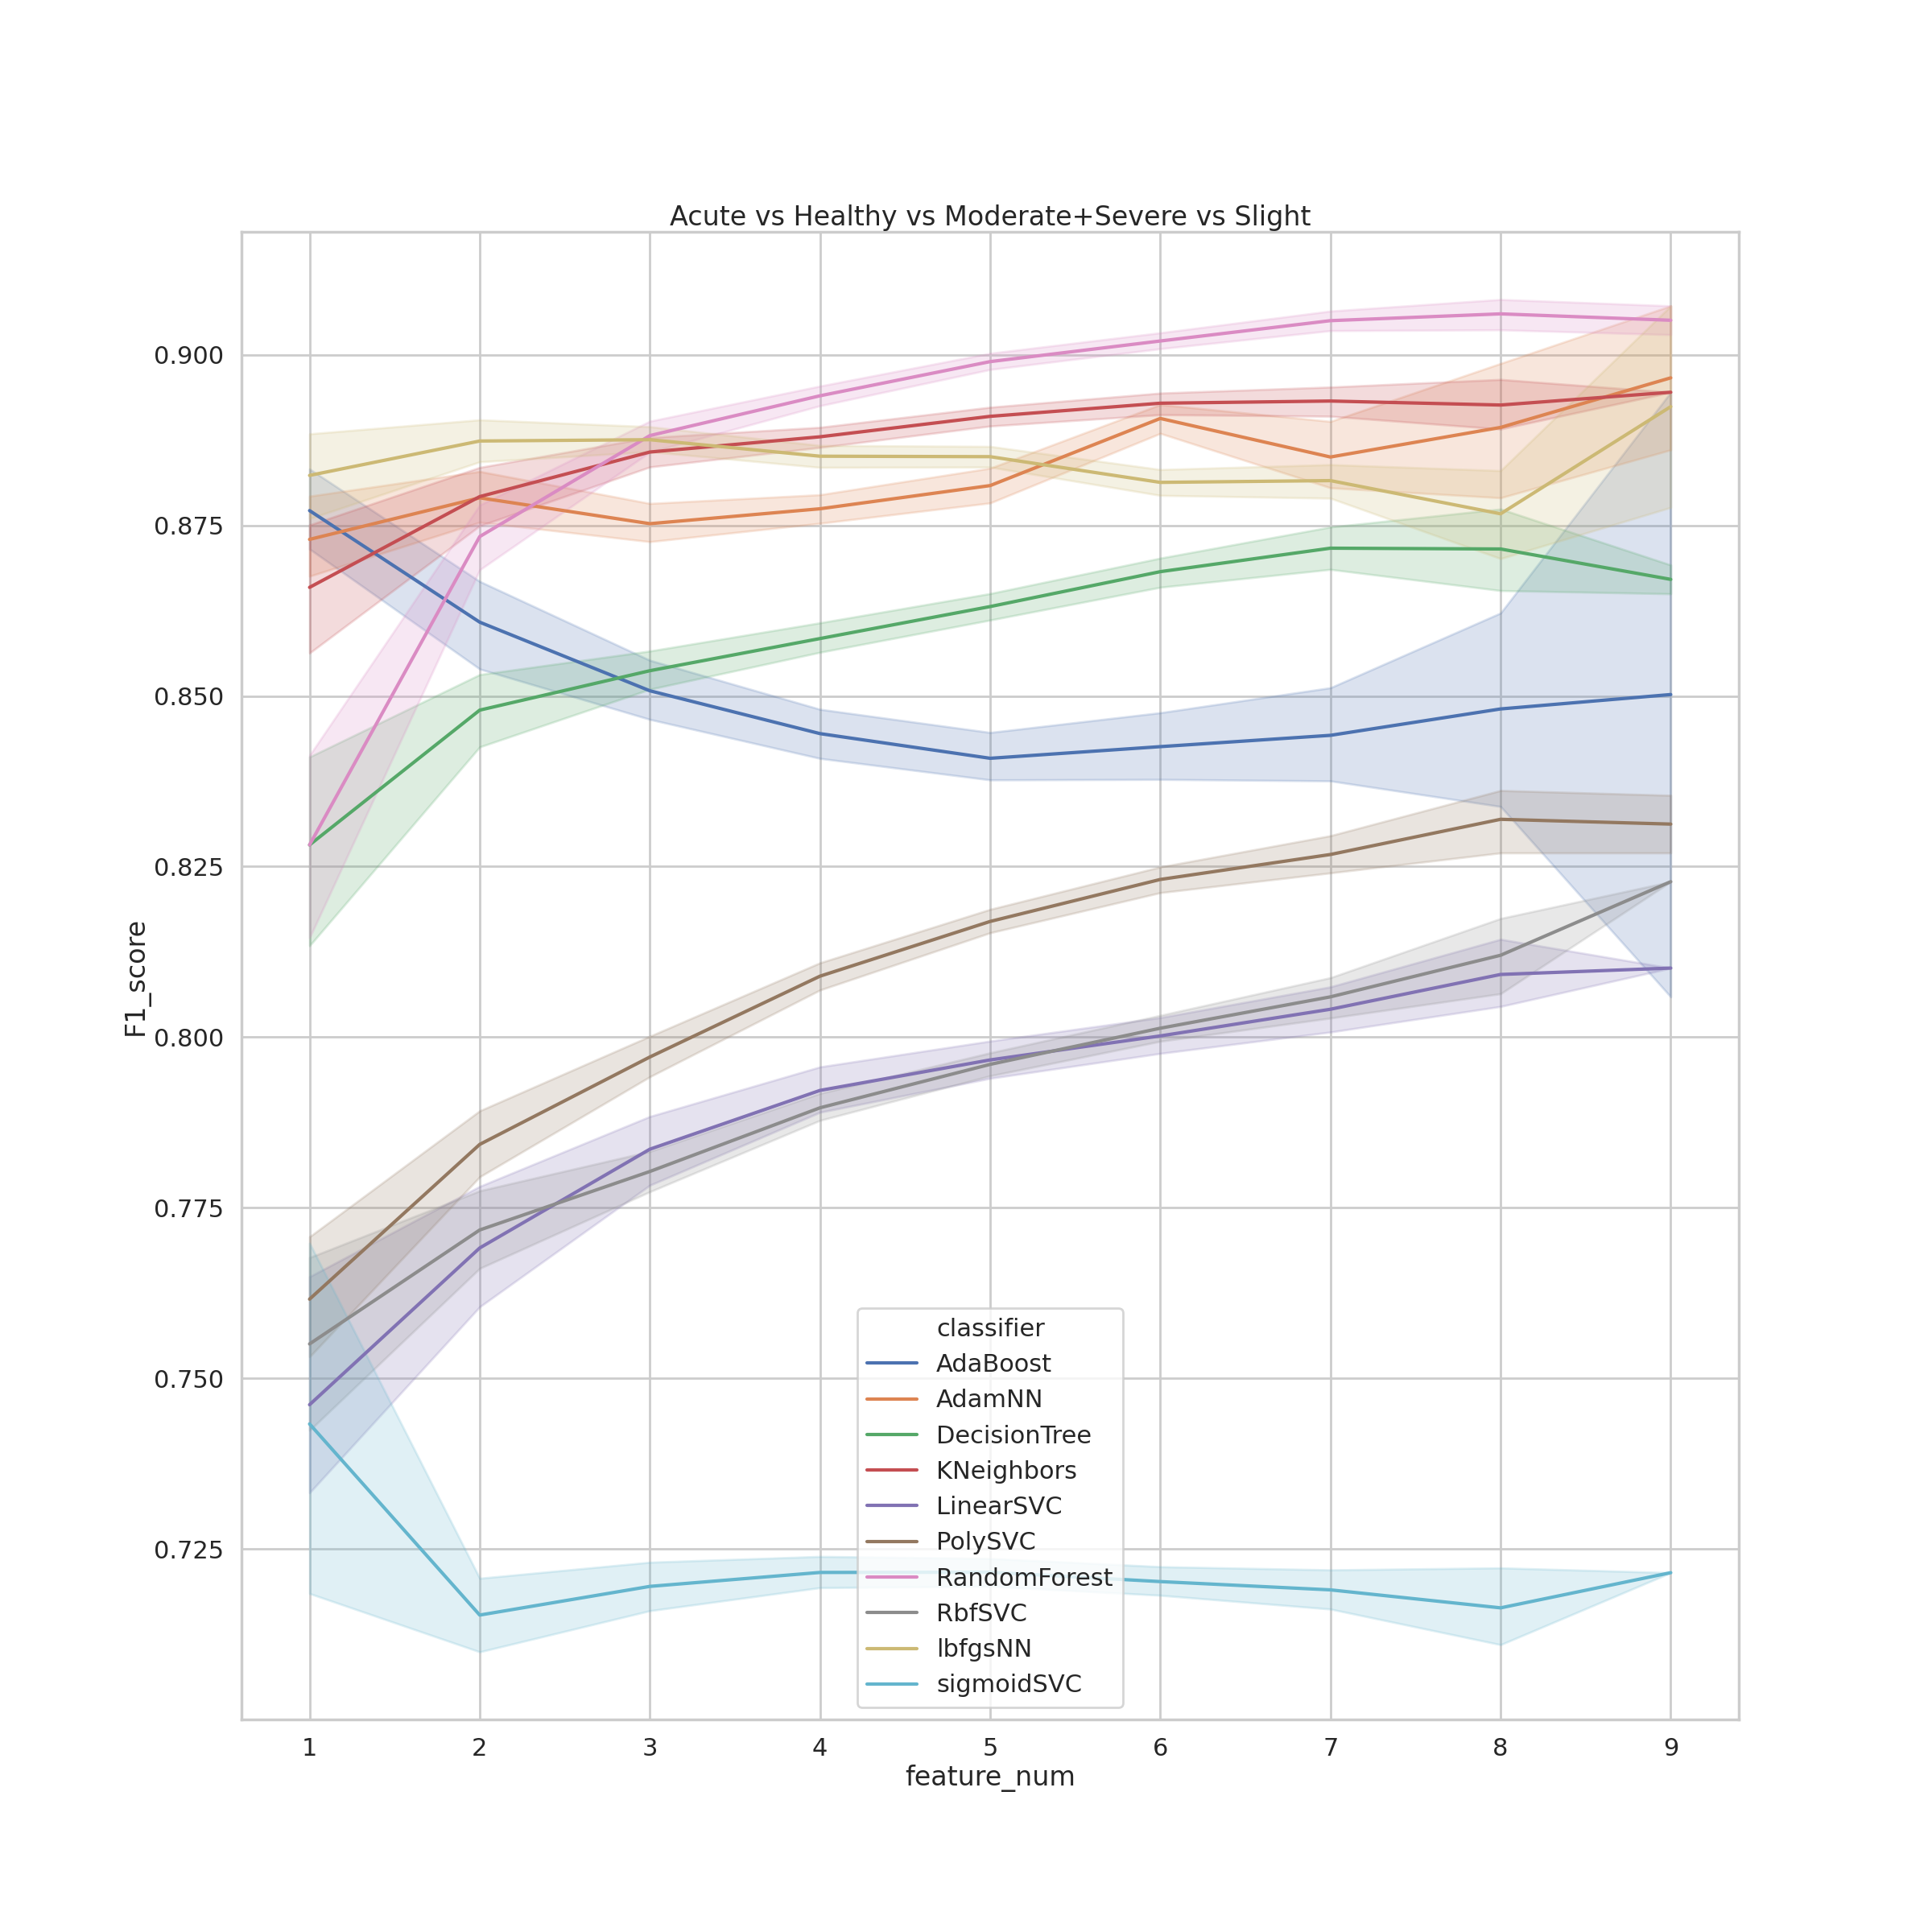
\includegraphics[width=0.3 \linewidth]{figures/Moderate-Severe/F1_score.png}
	    				&
	    				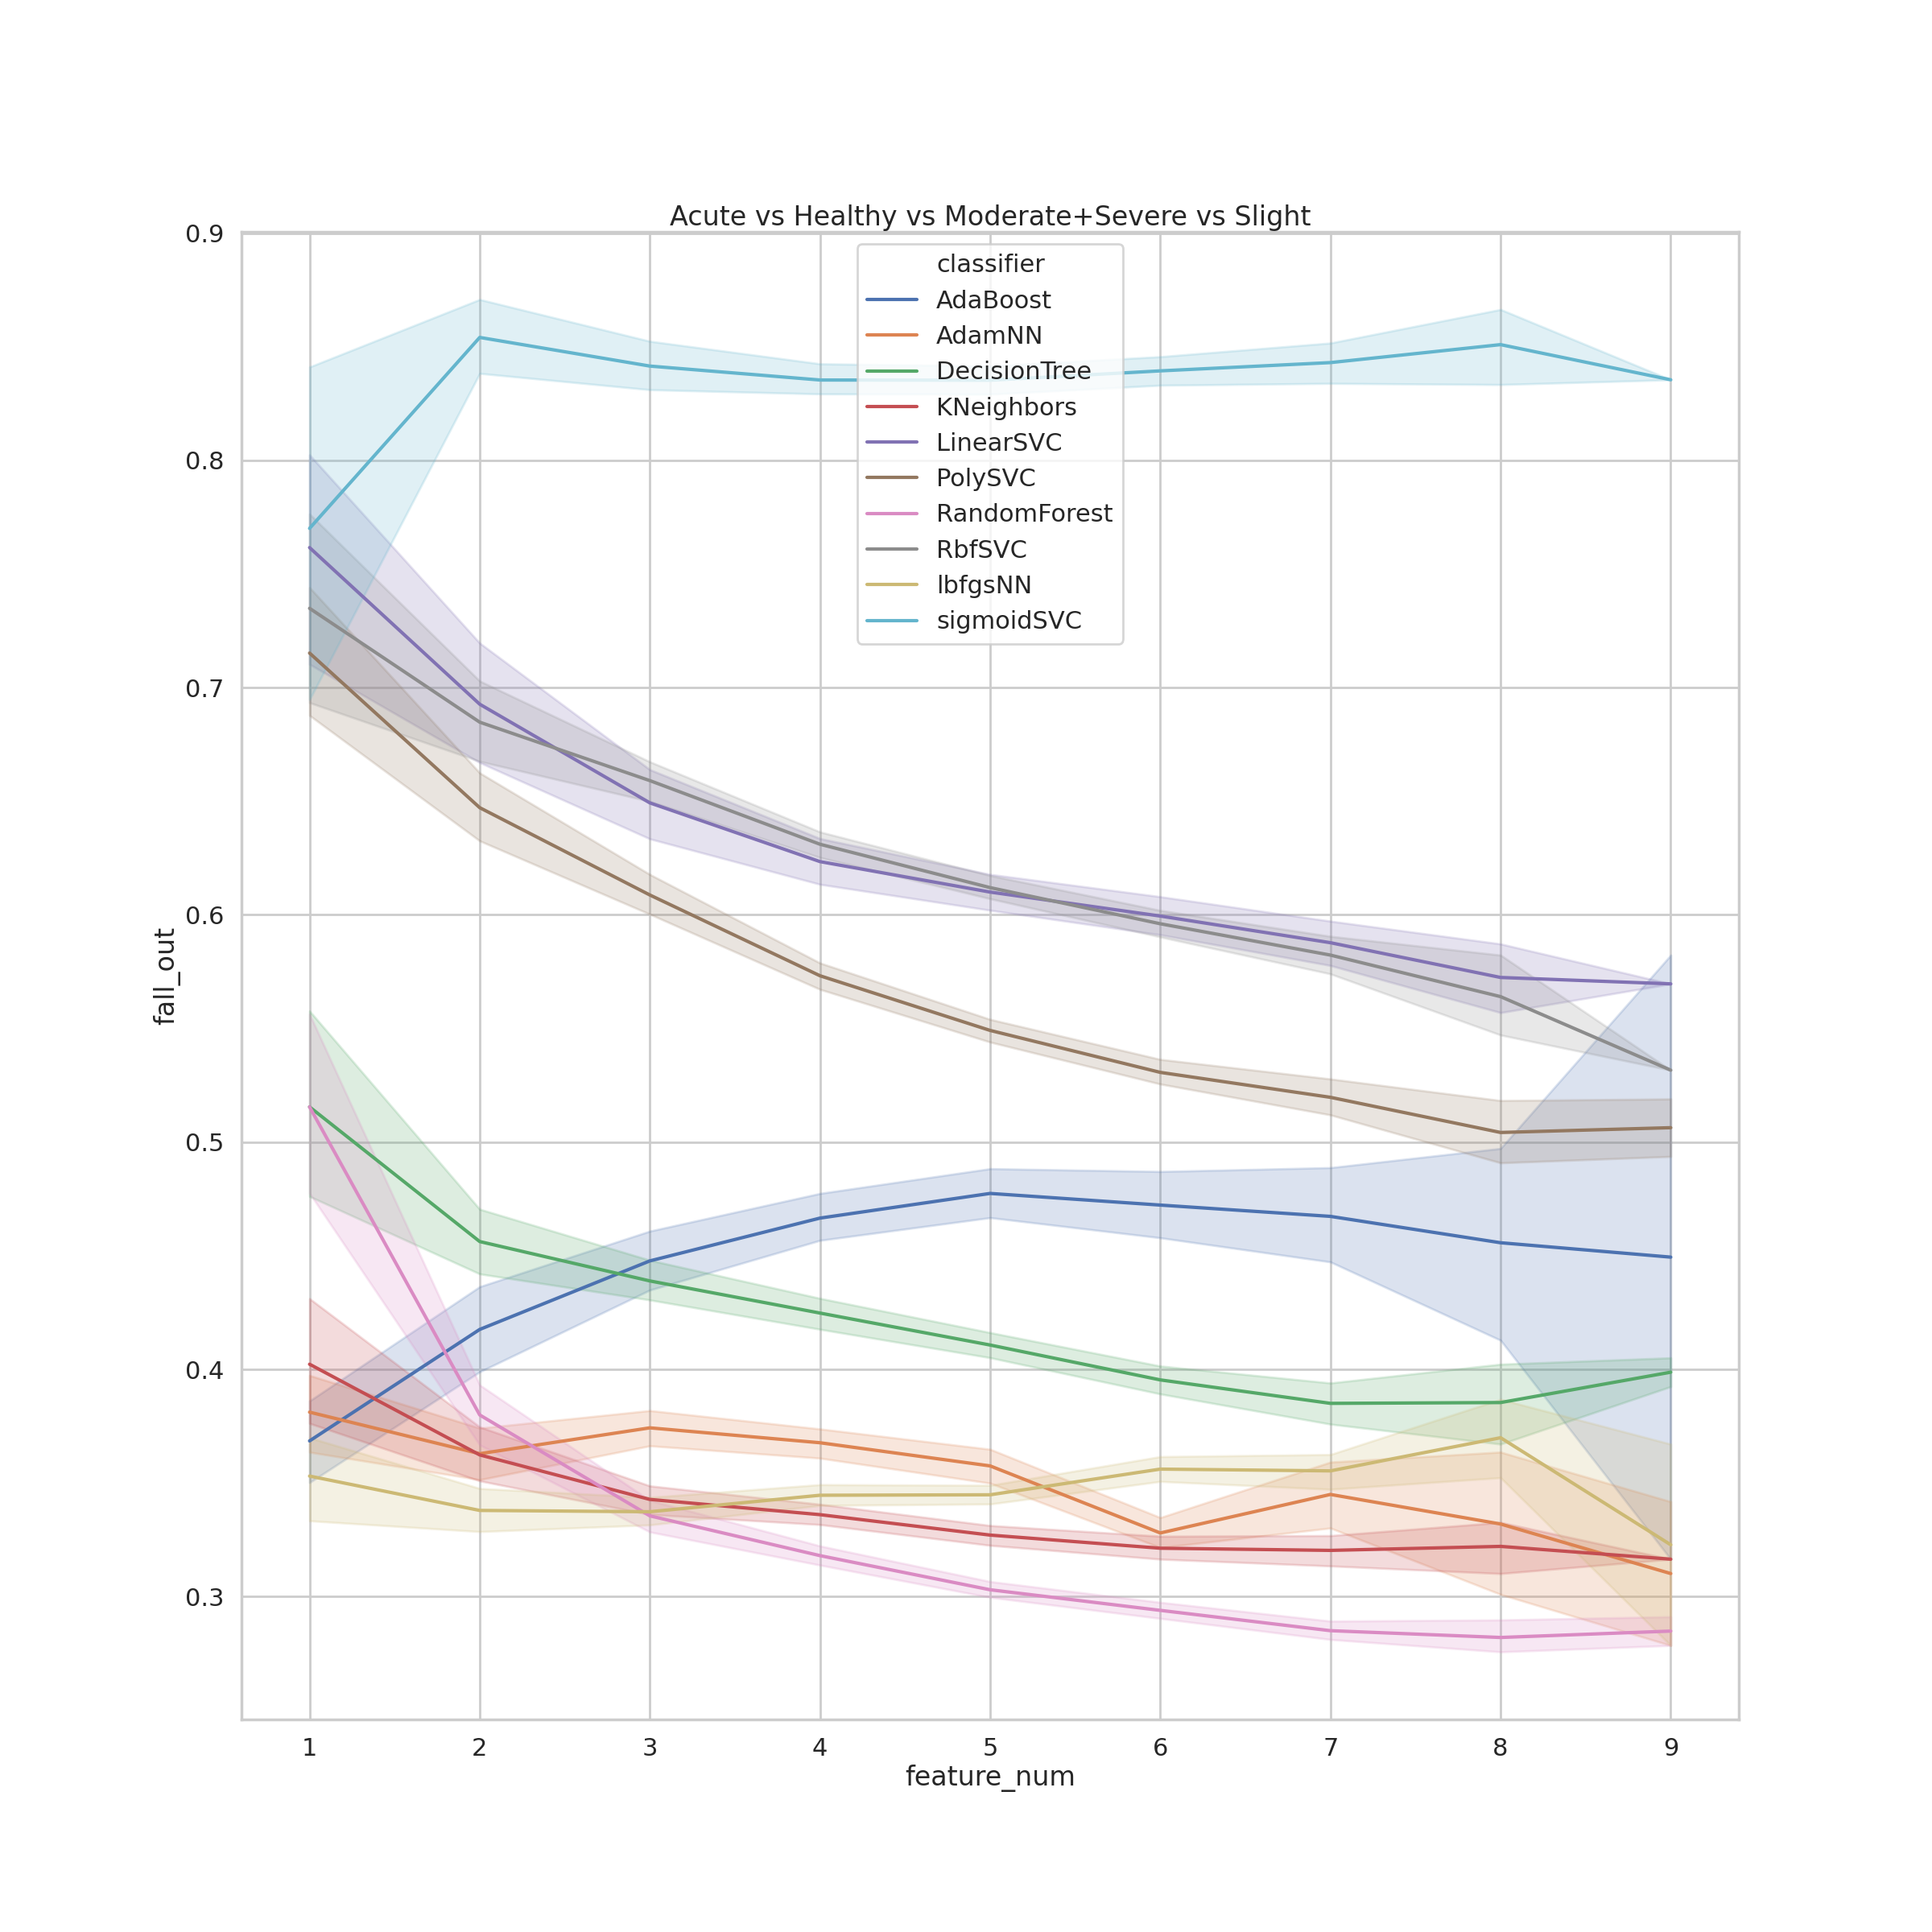
\includegraphics[width=0.3 \linewidth]{figures/Moderate-Severe/fall_out.png}
	    				\\
	    				\mbox{Accuracy} & \mbox{F1 score} & \mbox{Fall-out} \\
	    				
	    				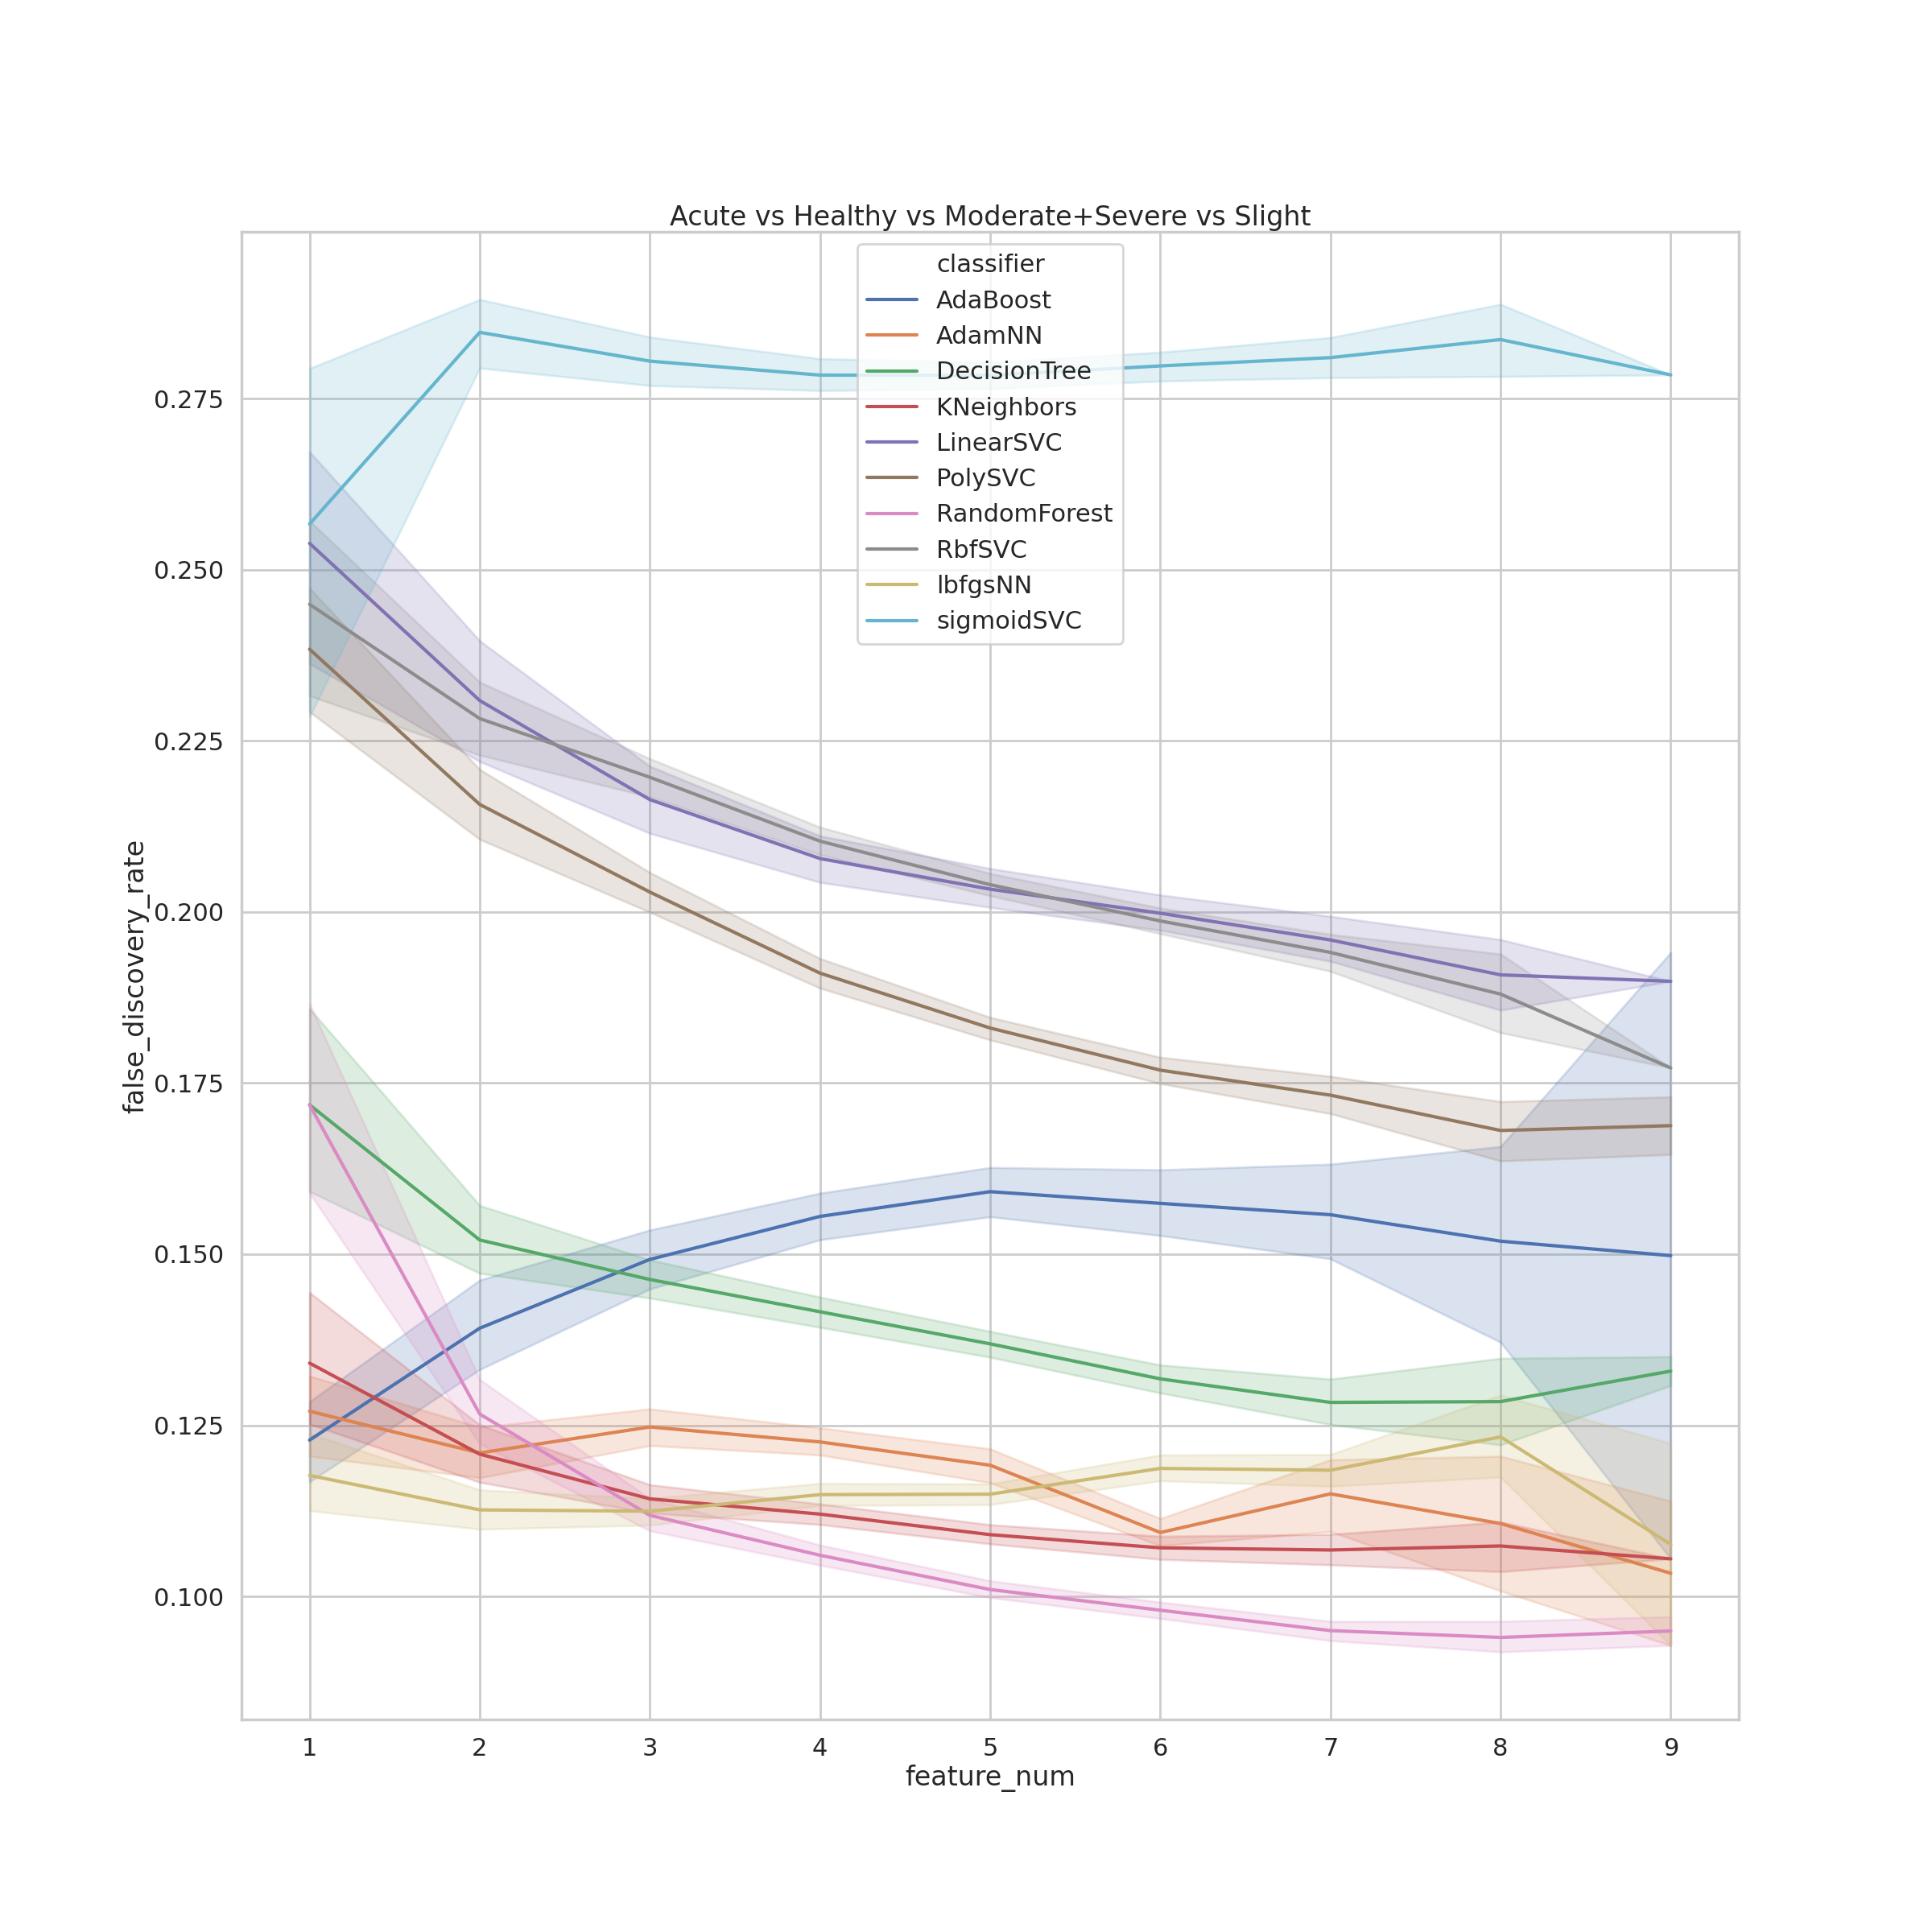
\includegraphics[width=0.3 \linewidth]{figures/Moderate-Severe/false_discovery_rate.png}
	    				&
	    				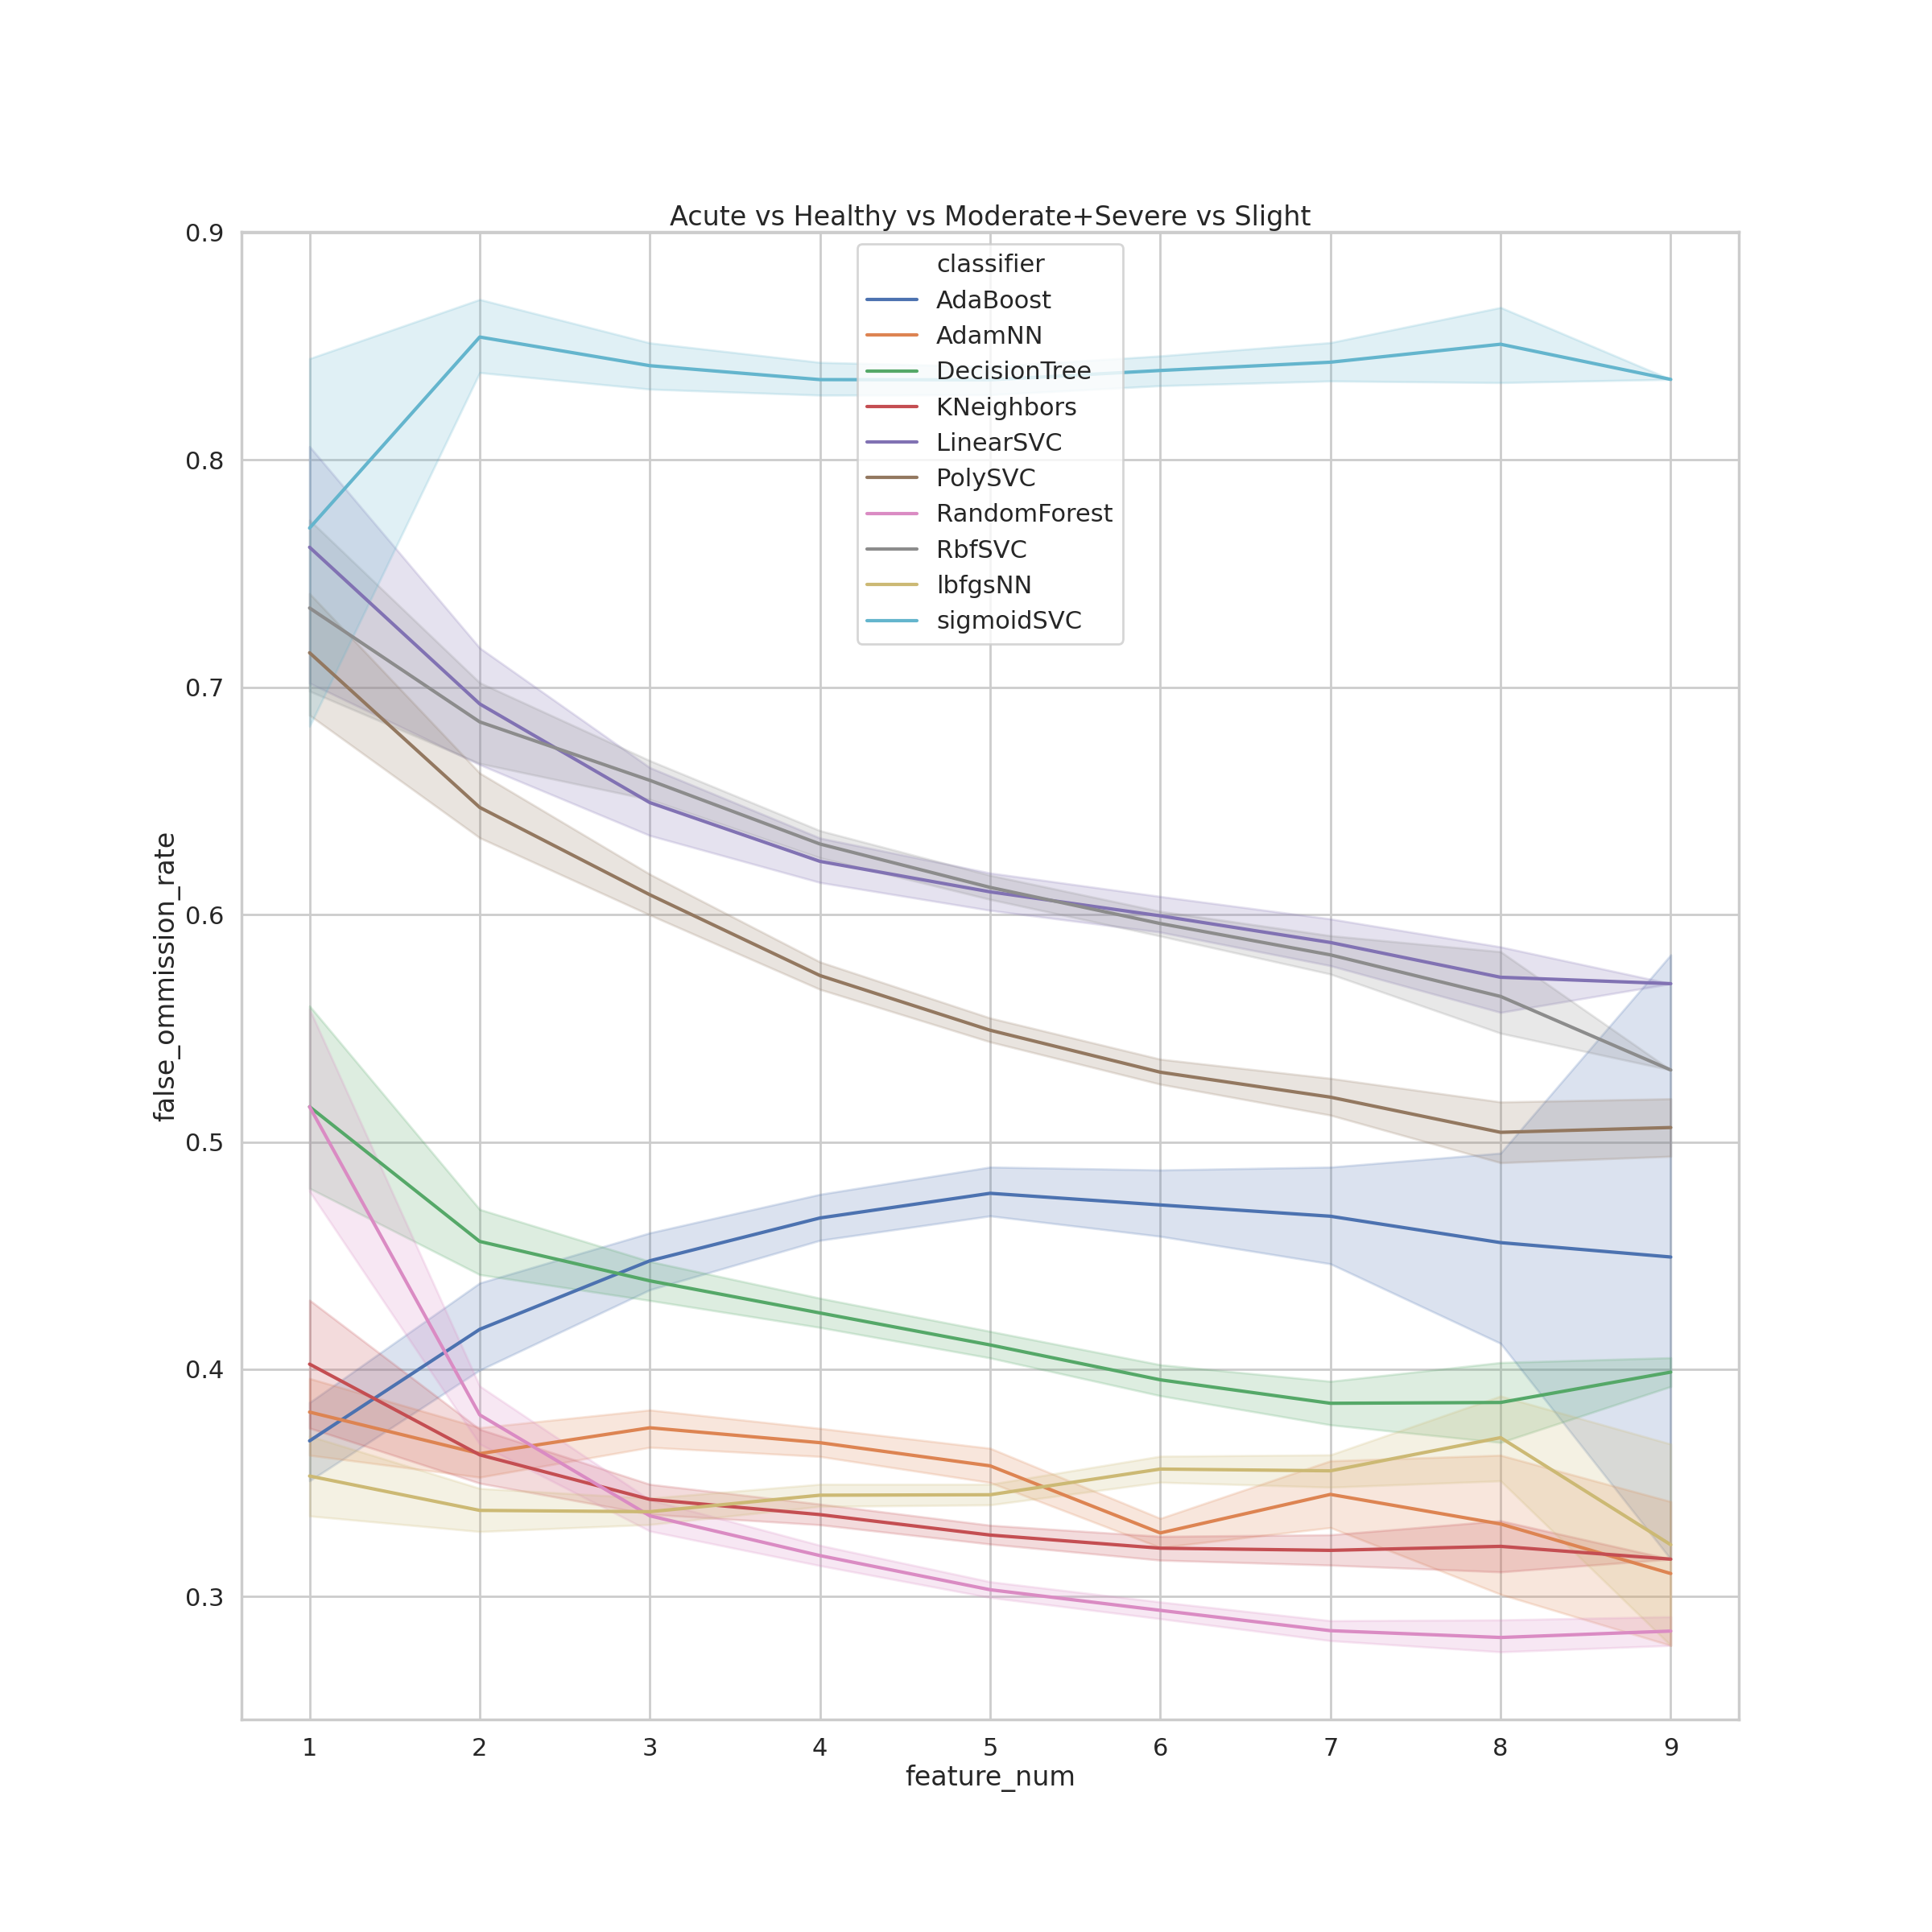
\includegraphics[width=0.3 \linewidth]{figures/Moderate-Severe/false_ommission_rate.png}
	    				&
	    				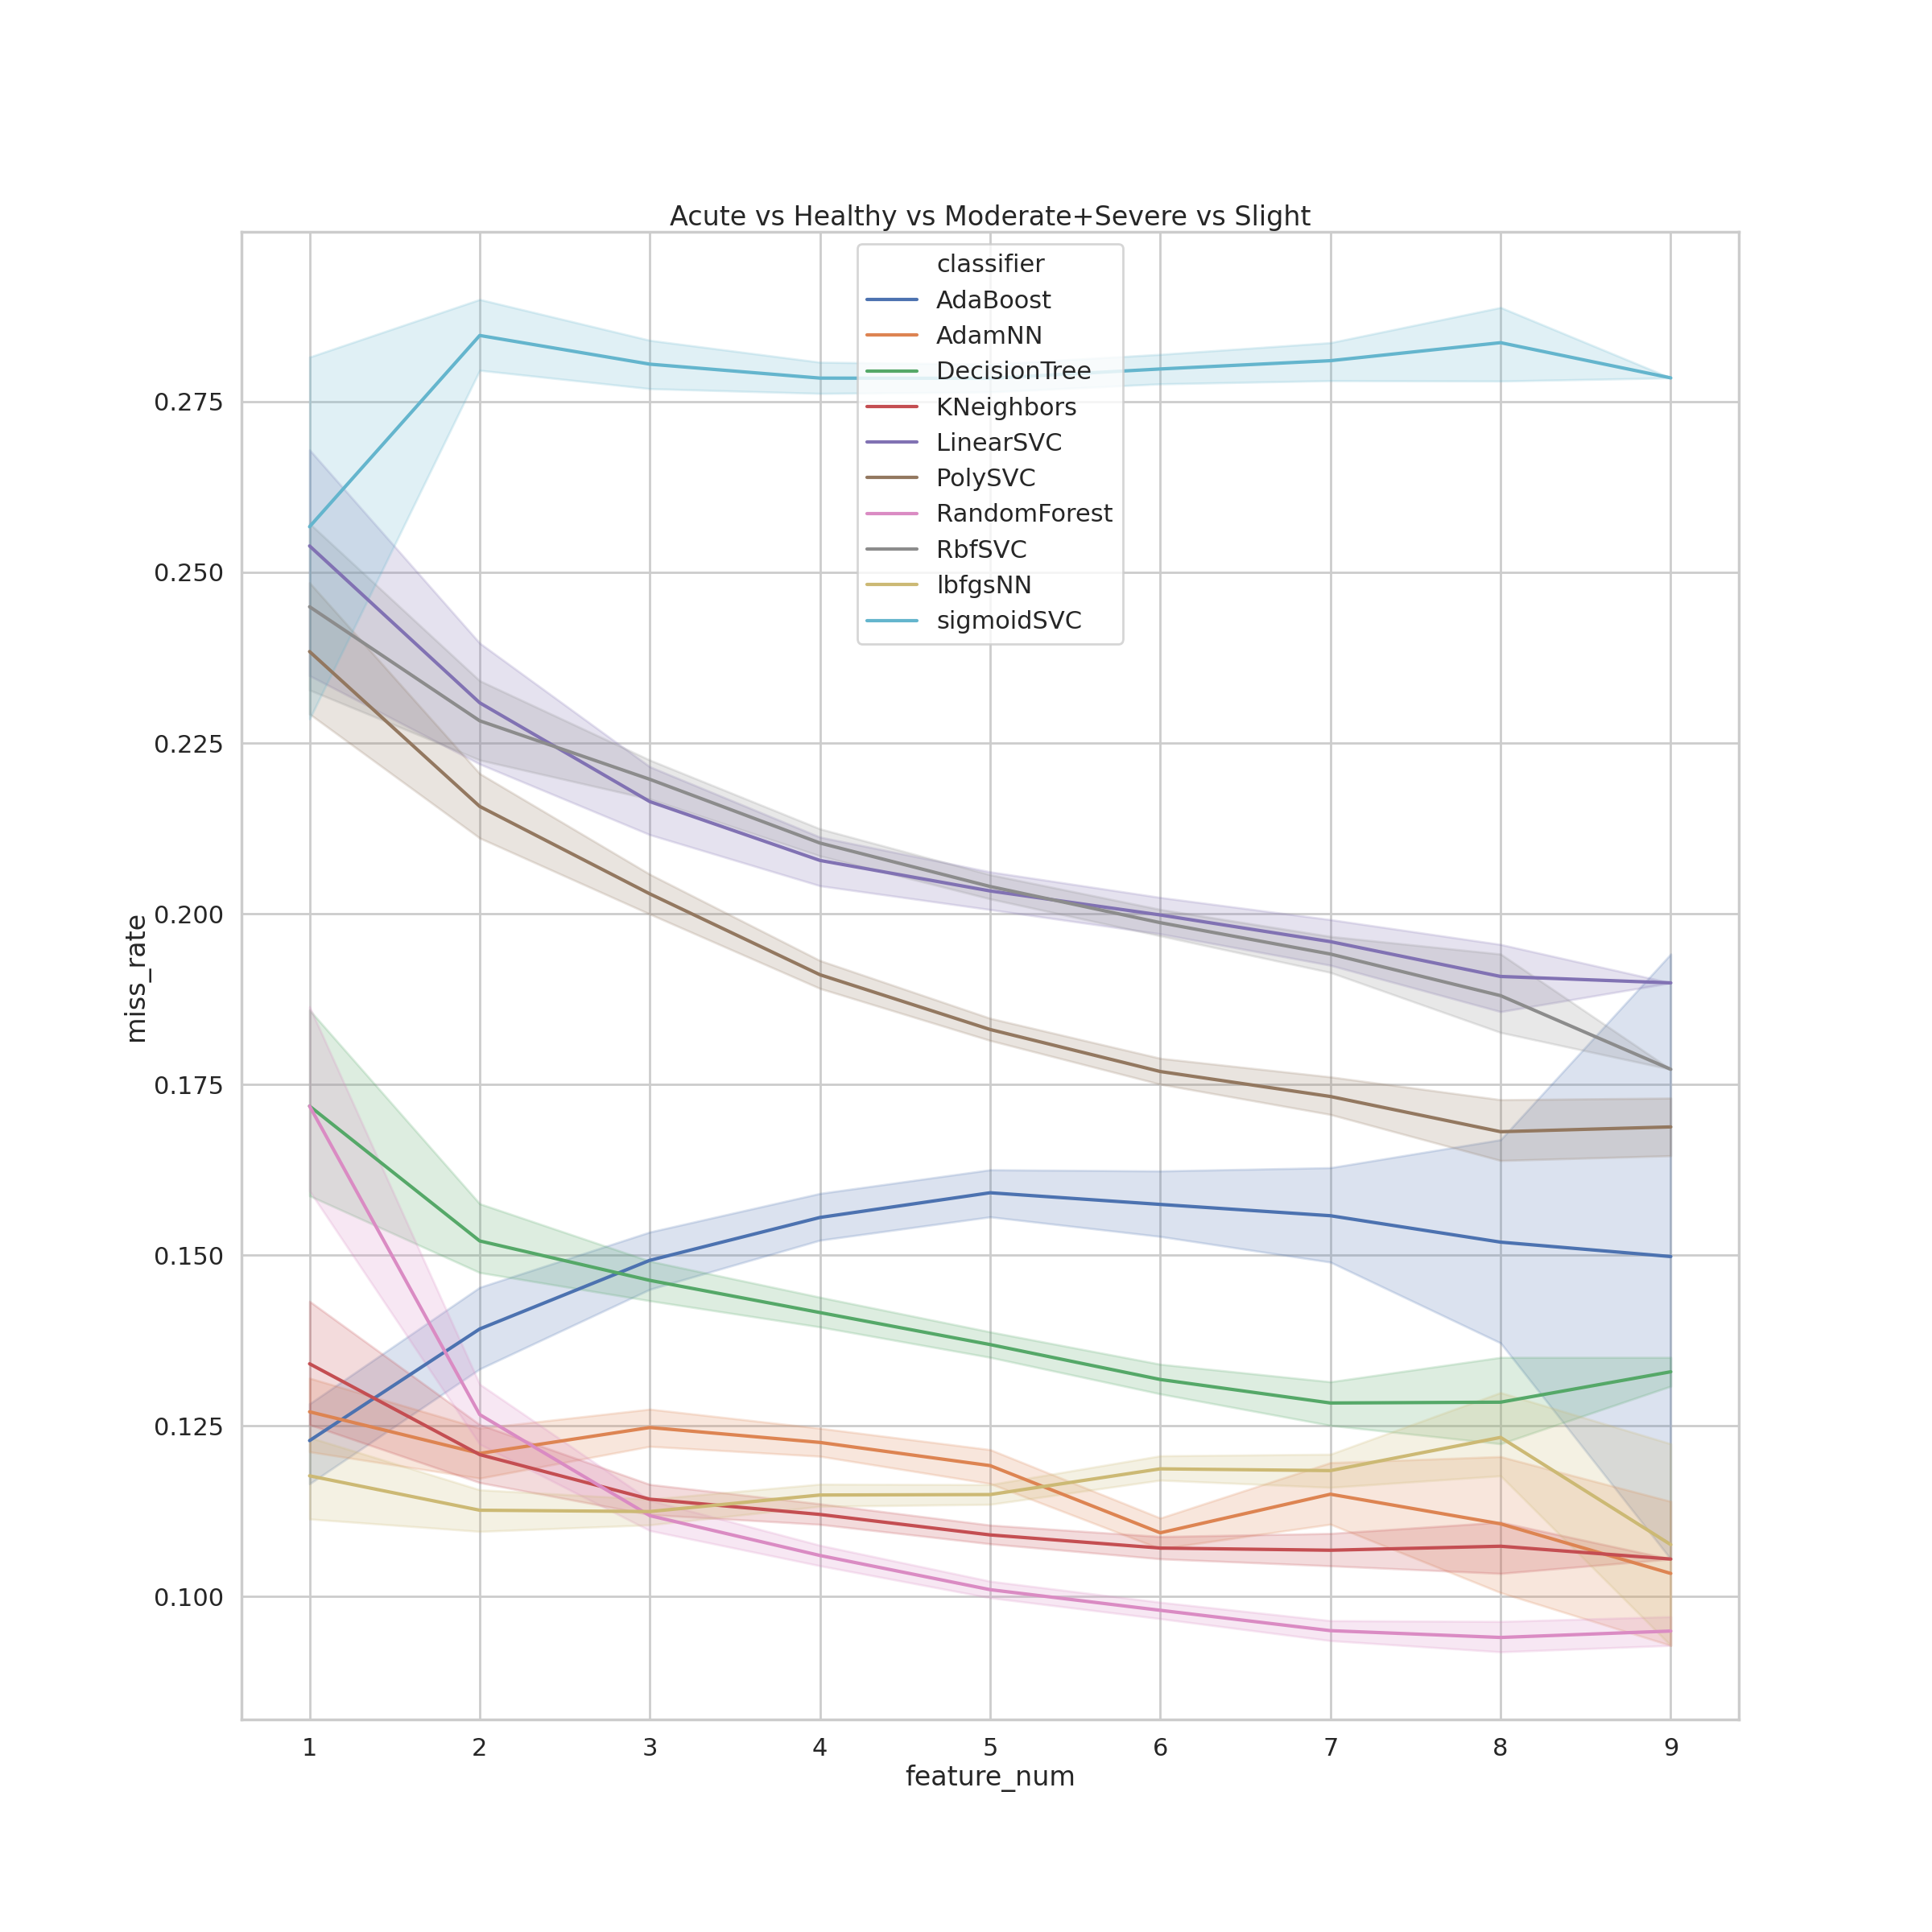
\includegraphics[width=0.3 \linewidth]{figures/Moderate-Severe/miss_rate.png}
	    				\\
	    				\mbox{False discovery rate} & \mbox{False ommision rate} & \mbox{Miss rate} \\ 
	    				
	    				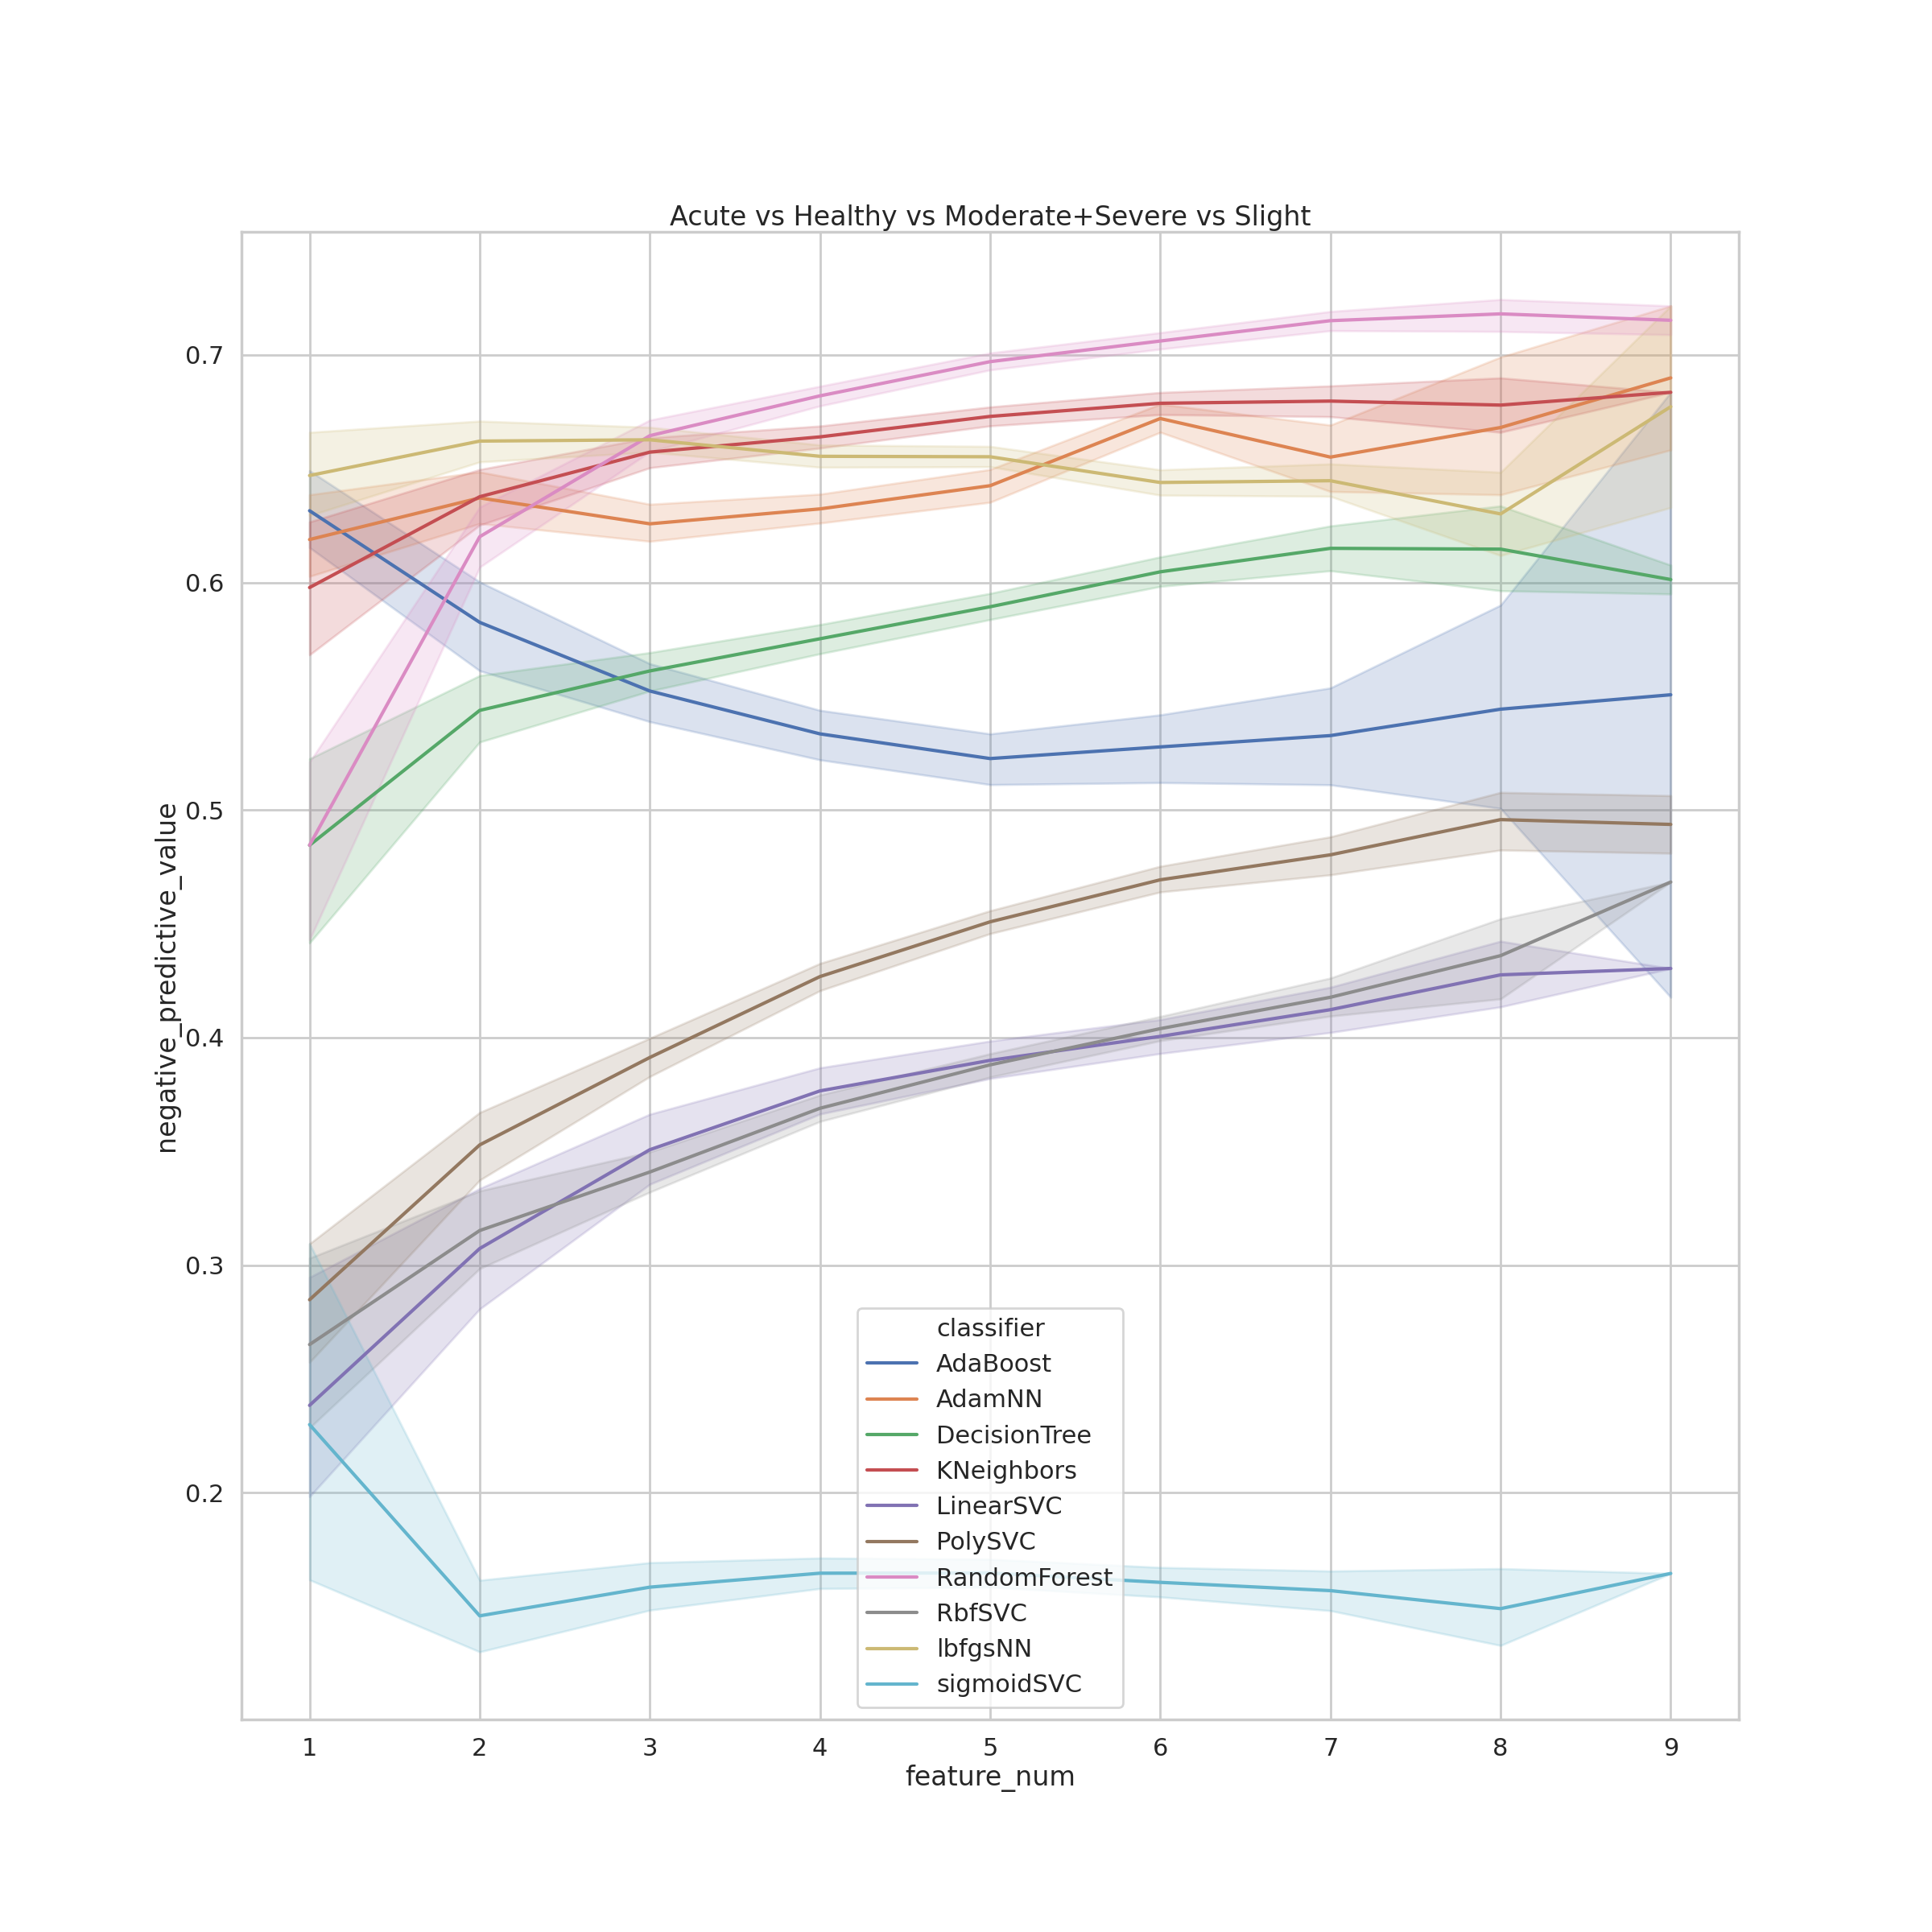
\includegraphics[width=0.3 \linewidth]{figures/Moderate-Severe/negative_predictive_value.png}
	    				&
	    				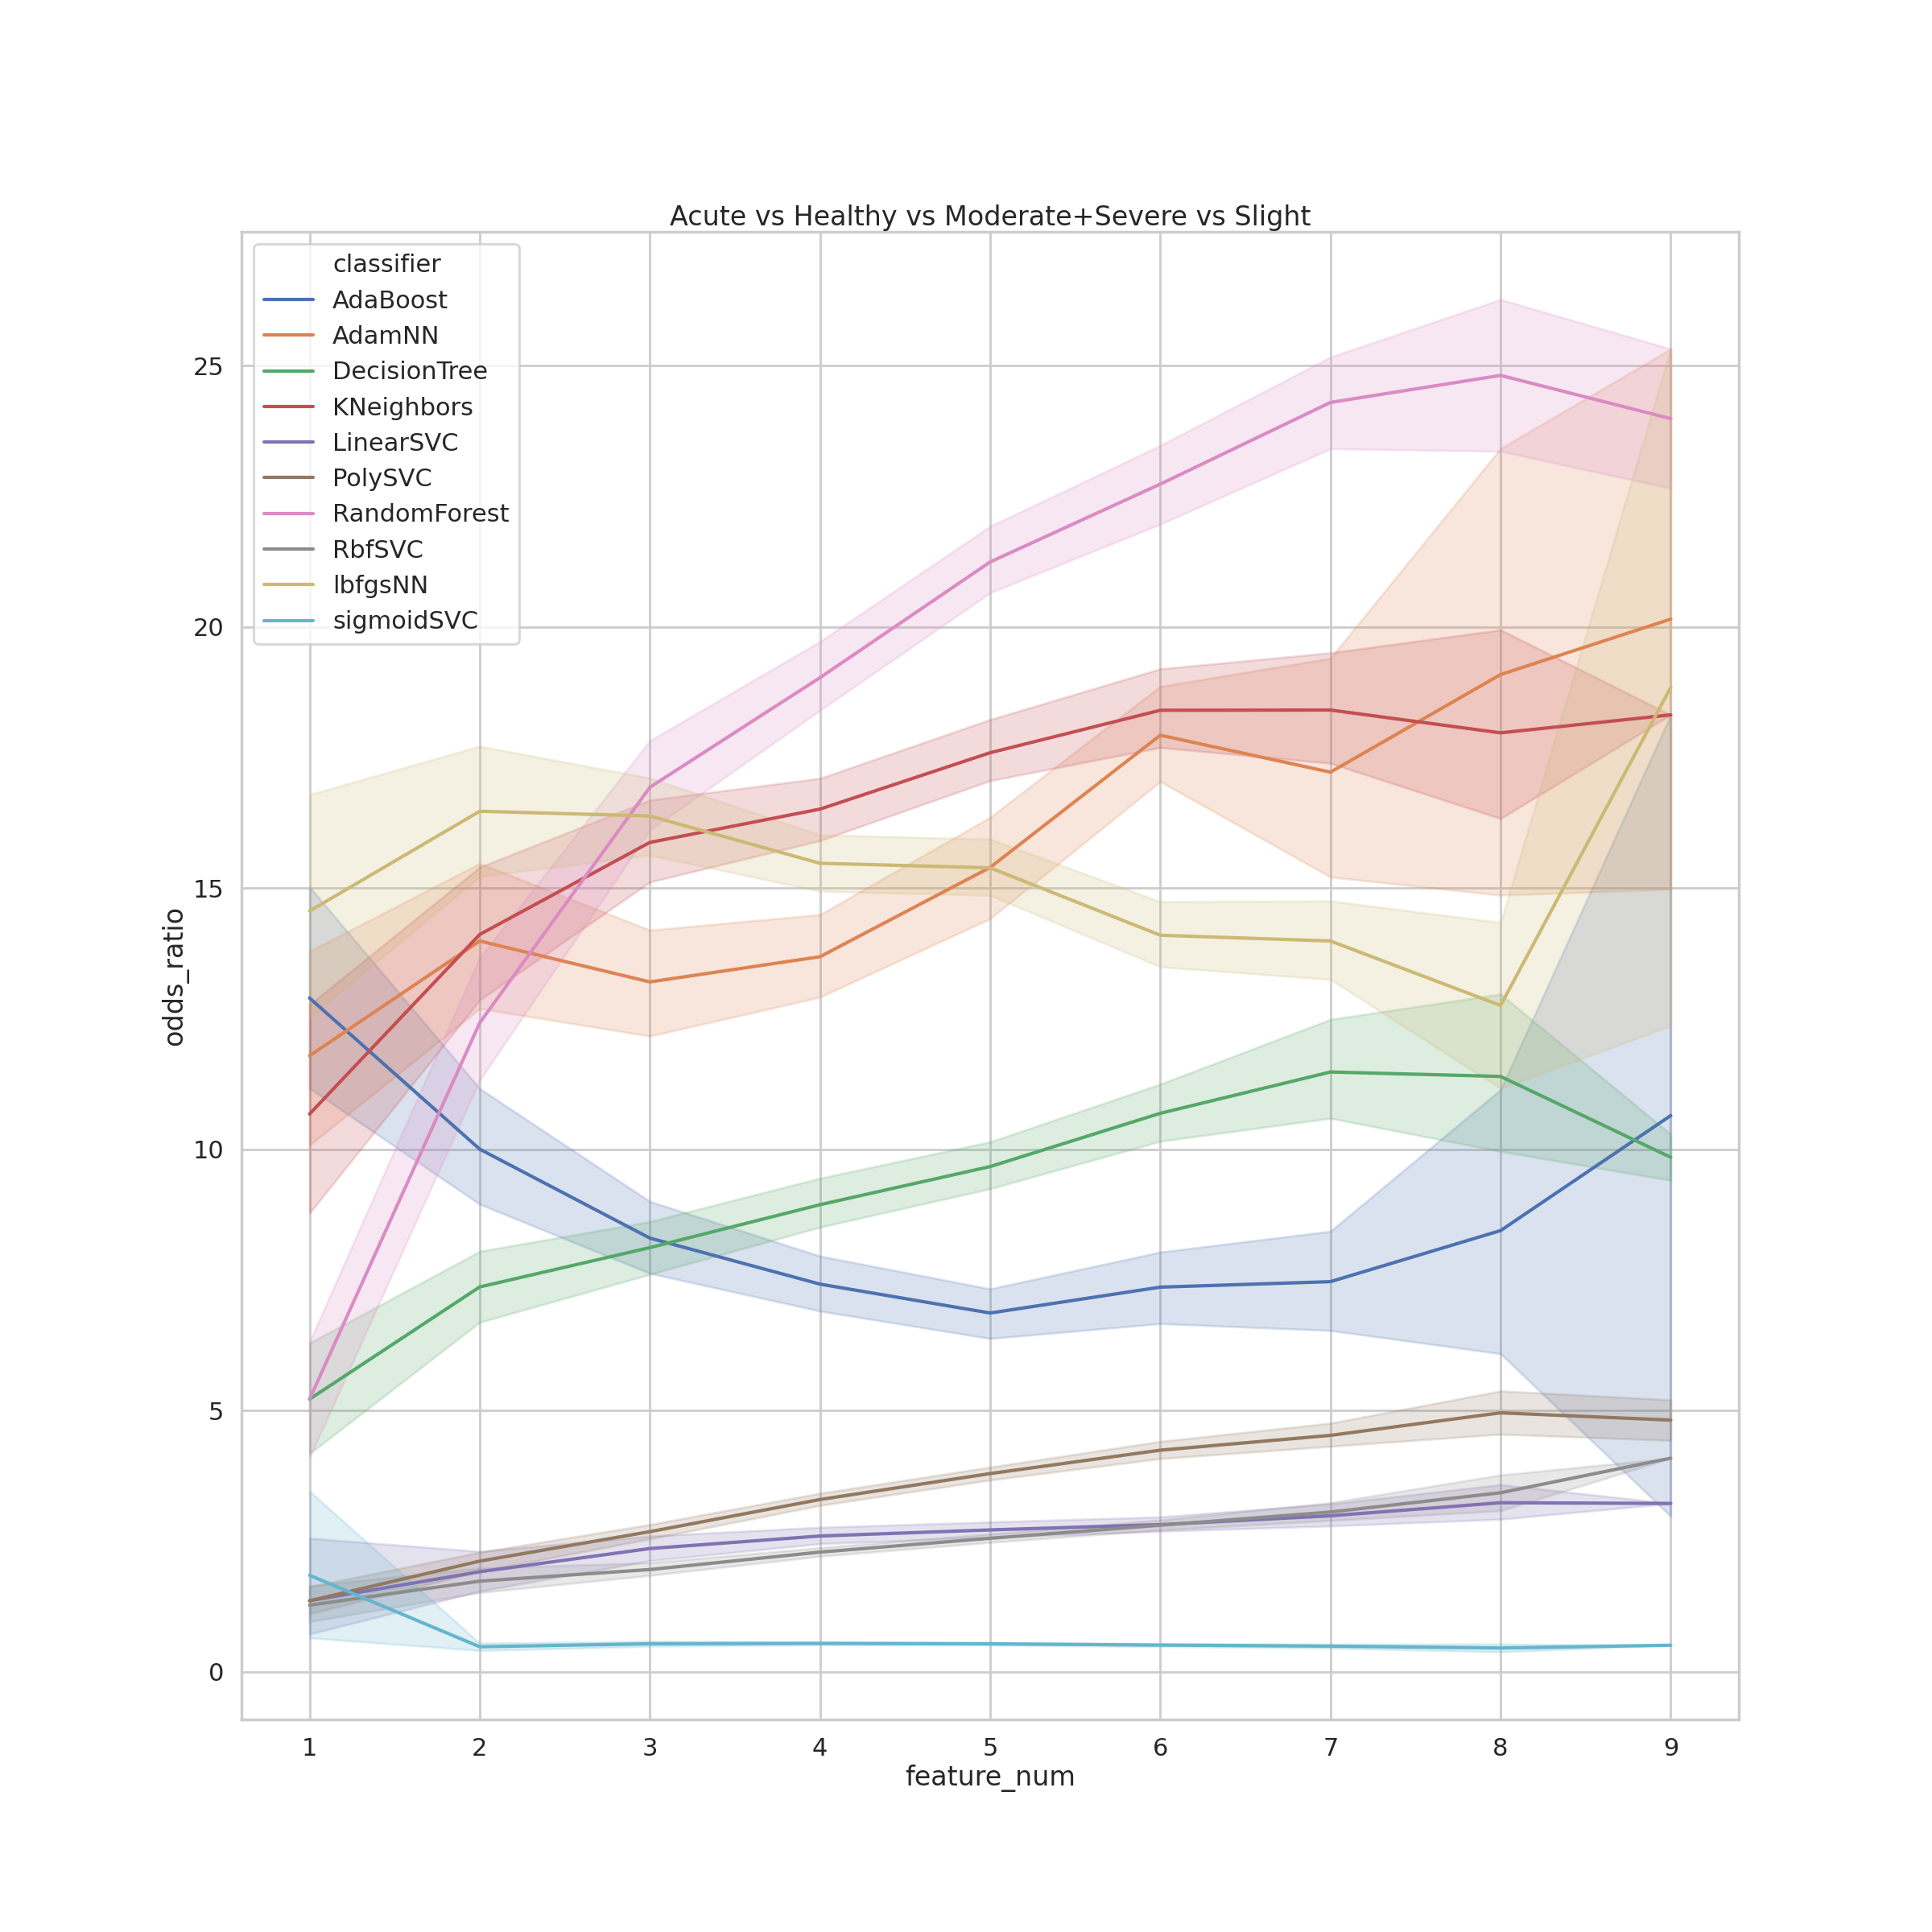
\includegraphics[width=0.3 \linewidth]{figures/Moderate-Severe/odds_ratio.png}
	    				&
	    				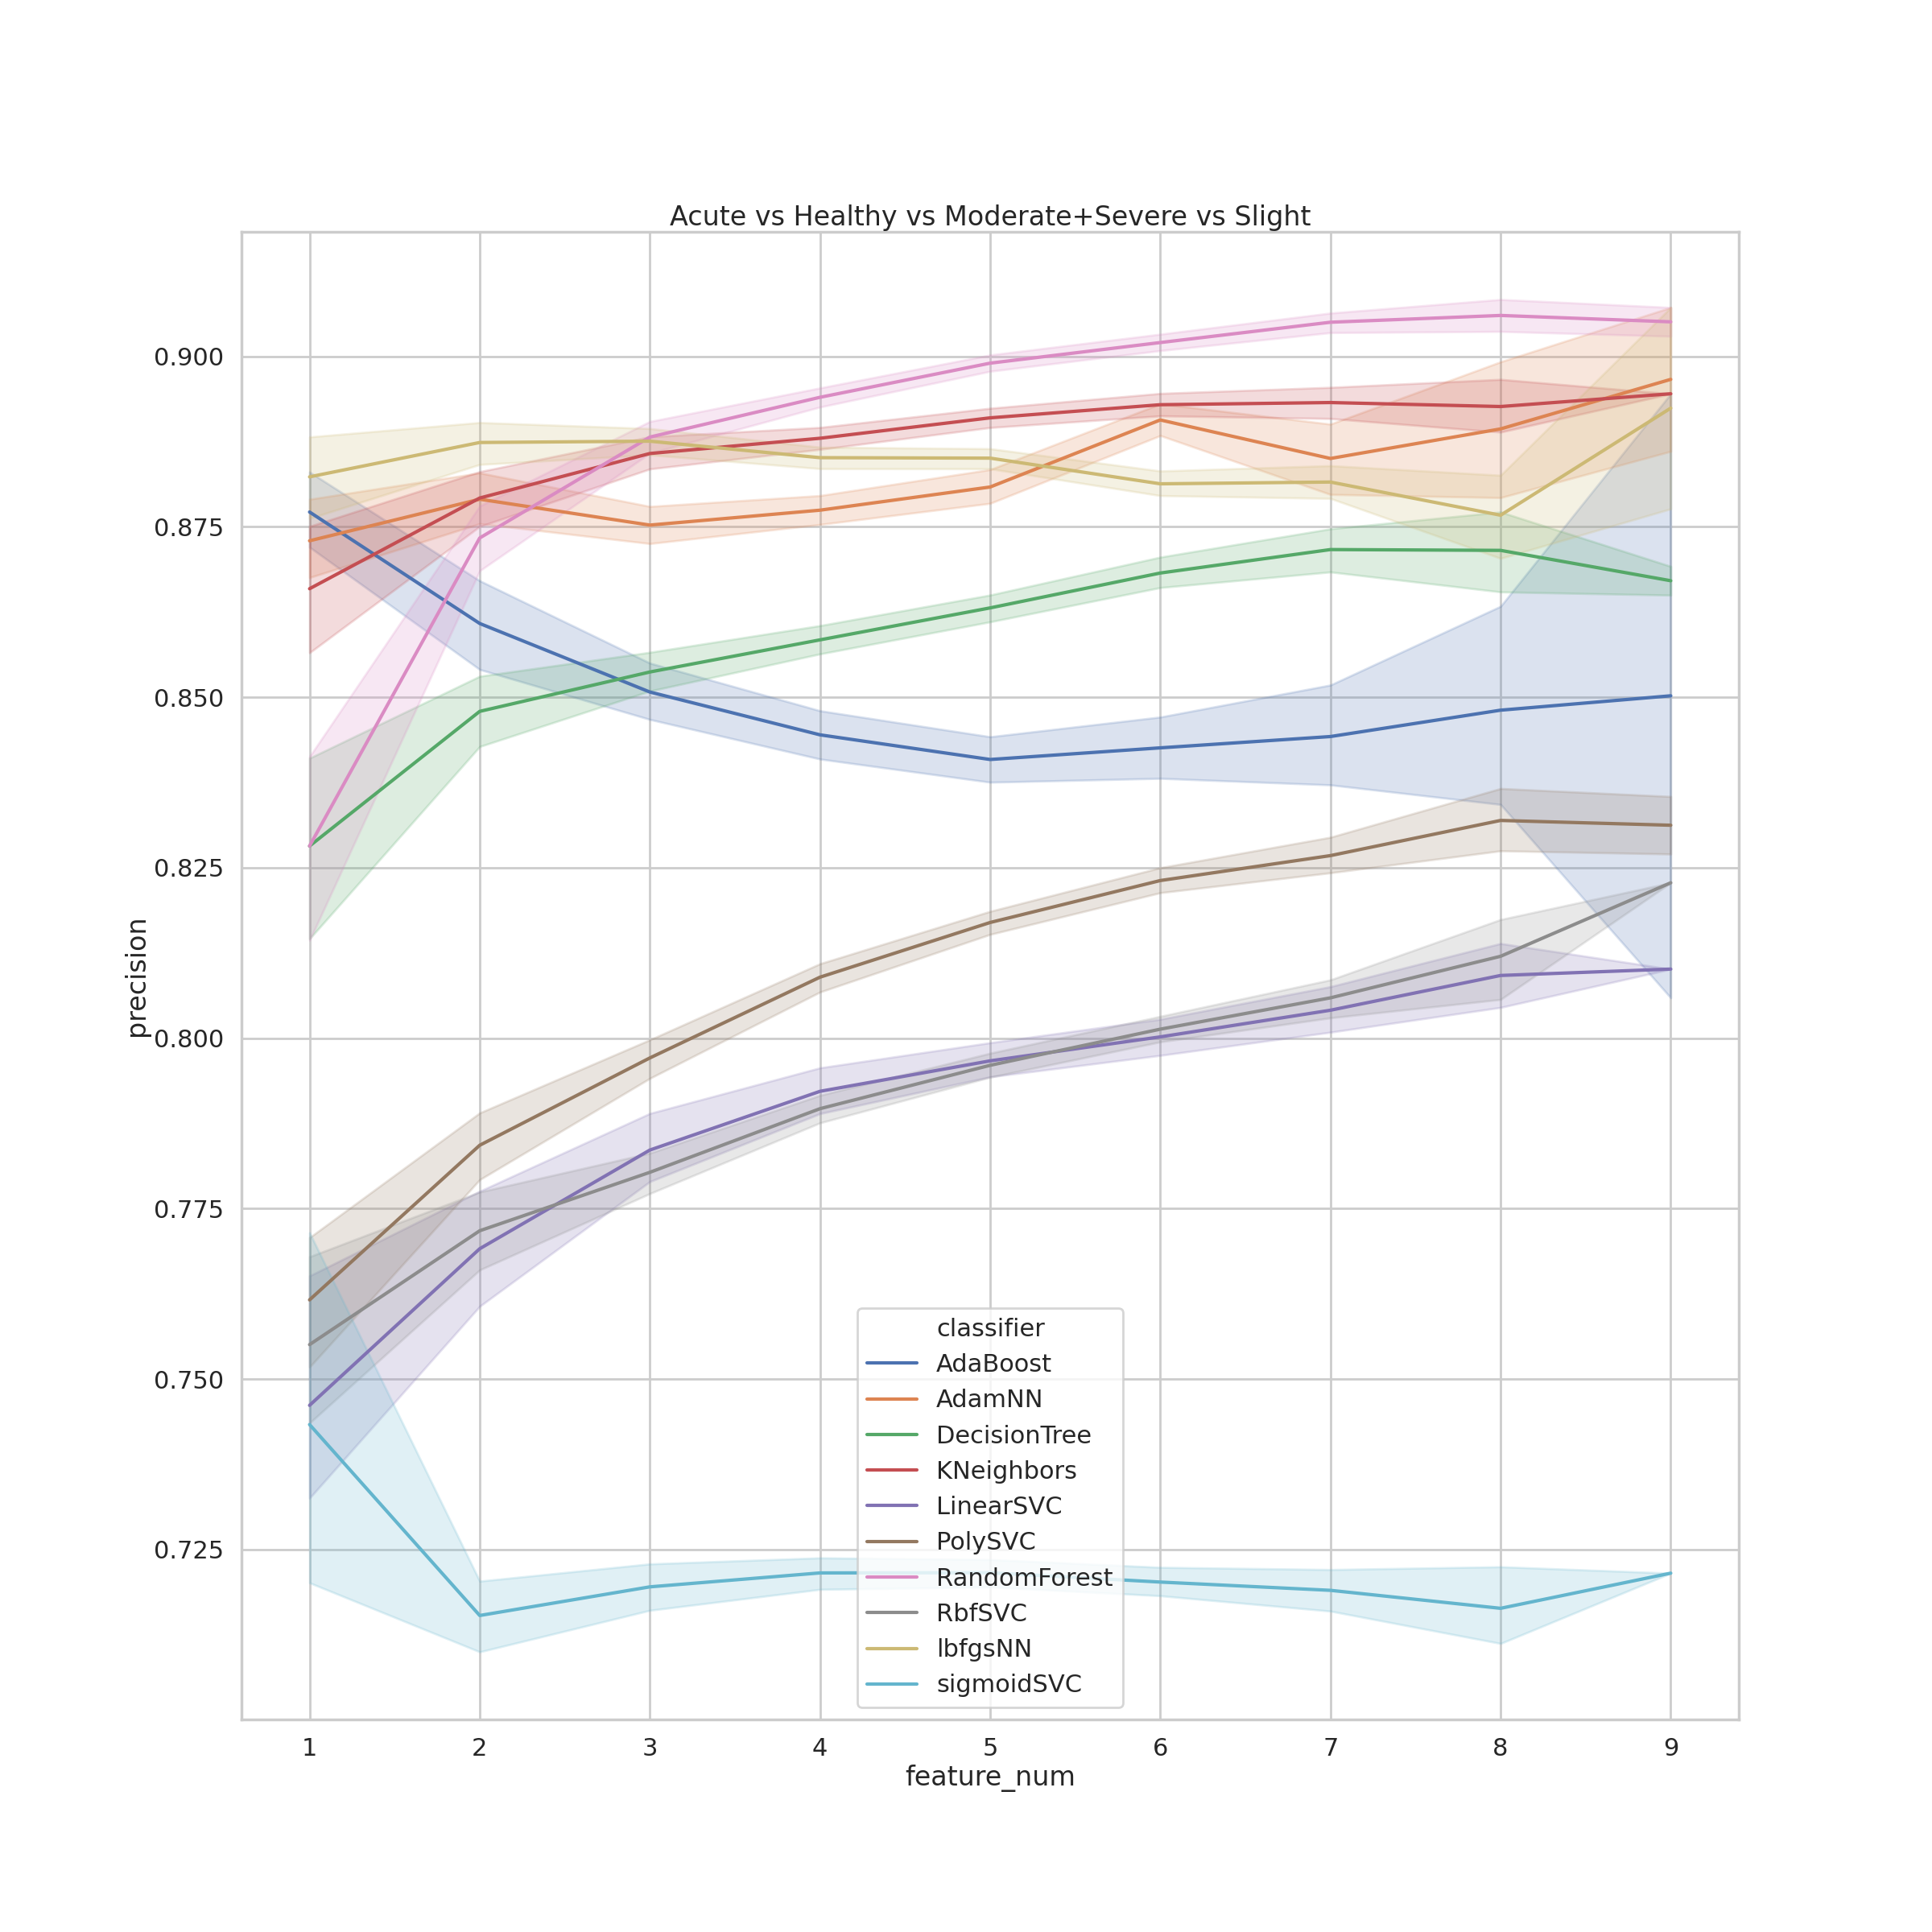
\includegraphics[width=0.3 \linewidth]{figures/Moderate-Severe/precision.png}
	    				\\
	    				\mbox{Negative predictive value} & \mbox{Odds ratio} & \mbox{Precision} \\ 
	    				
	    				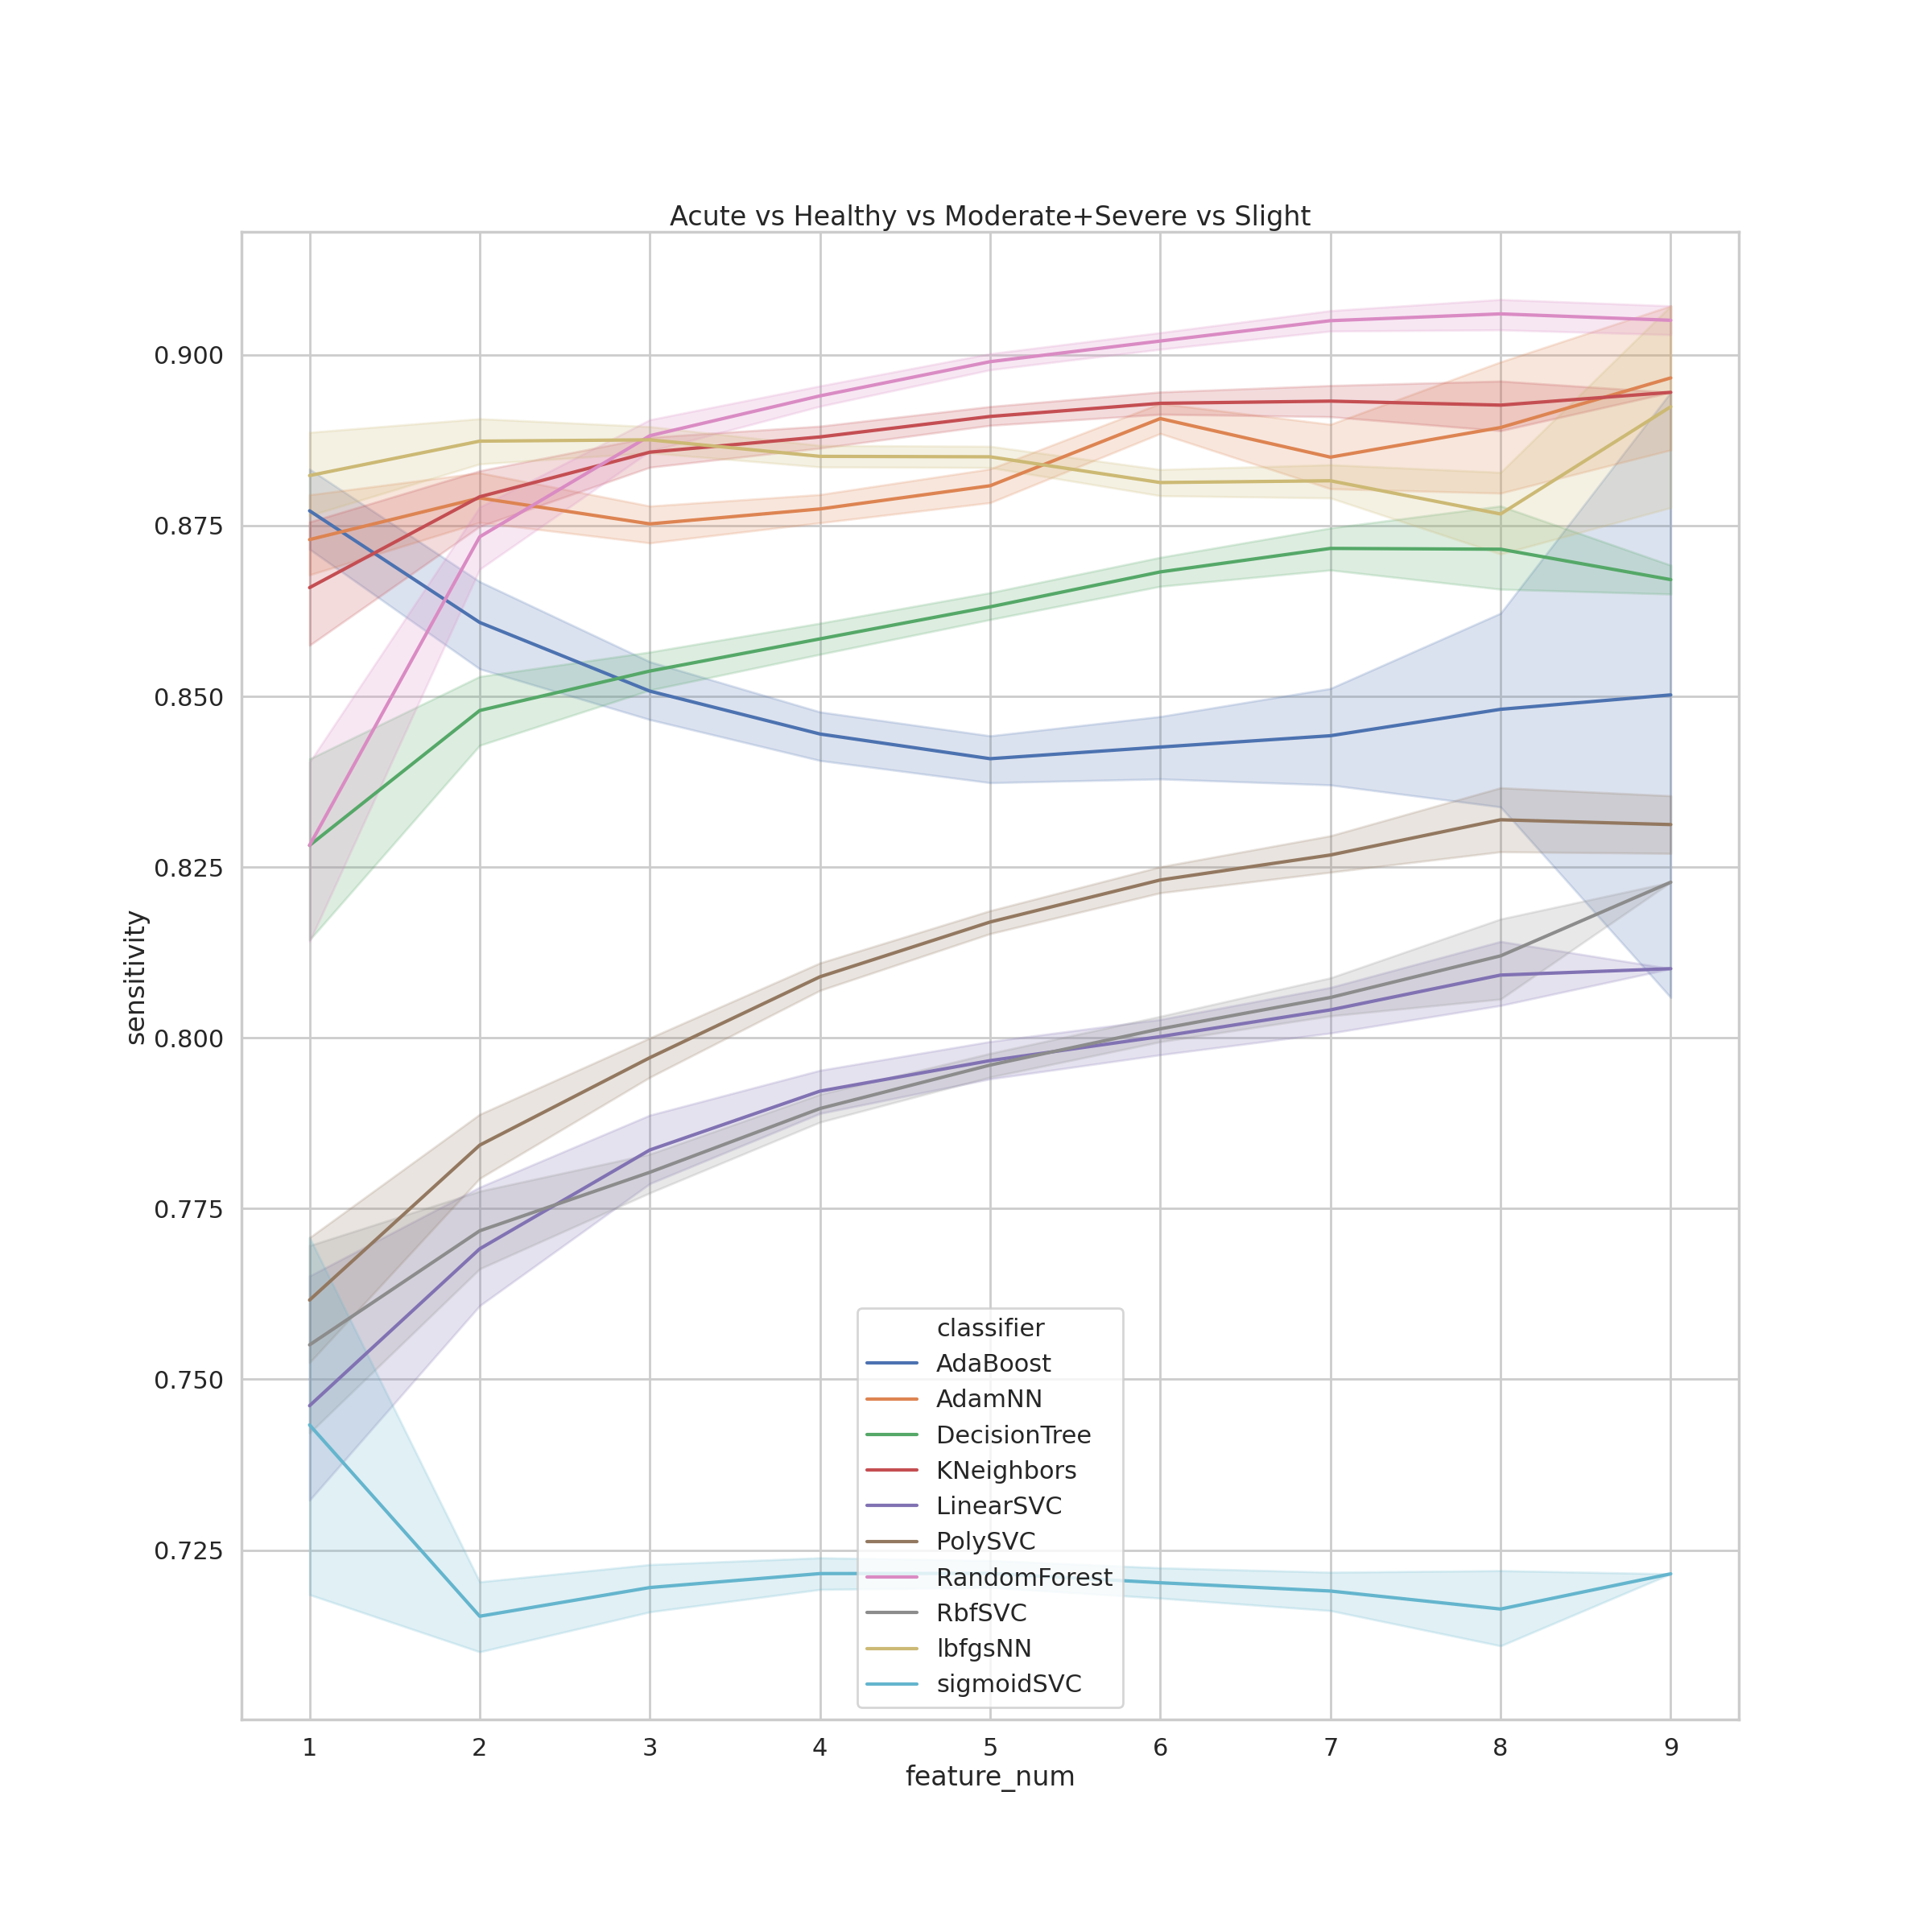
\includegraphics[width=0.3 \linewidth]{figures/Moderate-Severe/sensitivity.png}
	    				&
	    				\includegraphics[width=0.3 \linewidth]{figures/Moderate-Severe/specificity.png}
	    				&
	    				\includegraphics[width=0.3 \linewidth]{figures/Moderate-Severe/thread_score.png}
	    				\\
	    				\mbox{Sensitivity} & \mbox{Specificity} & \mbox{Thread score} \\
	    			\end{array}$
	    			\caption{Confusion Matrix Derivations from Moderate-Severe Classification}
	    			\label{fig:m-s-confusion}
    			\end{figure}
    			
    			\begin{figure}[htbp]
    				\centering
    				\includegraphics[width=0.5 \linewidth]{figures/Slight-Moderate/heatmap.png}
    				\caption{Heatmap Plot for Merged Slight-Moderate Classification with Random Forest}
    				\label{fig:m-s-heatmap}
    			\end{figure}
    		
    		\subsubsection{Merged Slight-Acute Class}
    			Figure \ref{fig:sli-a-confusion} displays the derivations of confusion matrix in merged slight-acute classification. Note that the values in figure \ref{fig:sli-a-confusion}, mean values from combination which used same number of features will be shown. As figure \ref{fig:sli-a-heatmap}, the Random Forest algorithm as the best values with all features. 
    		
    			\begin{figure}[htbp]
    				\centering
    				$\begin{array}{ccc}
	    				\includegraphics[width=0.3 \linewidth]{figures/Slight-Acute/accuracy.png}
	    				&
	    				\includegraphics[width=0.3 \linewidth]{figures/Slight-Acute/F1_score.png}
	    				&
	    				\includegraphics[width=0.3 \linewidth]{figures/Slight-Acute/fall_out.png}
	    				\\
	    				\mbox{Accuracy} & \mbox{F1 score} & \mbox{Fall-out} \\
	    				
	    				\includegraphics[width=0.3 \linewidth]{figures/Slight-Acute/false_discovery_rate.png}
	    				&
	    				\includegraphics[width=0.3 \linewidth]{figures/Slight-Acute/false_ommission_rate.png}
	    				&
	    				\includegraphics[width=0.3 \linewidth]{figures/Slight-Acute/miss_rate.png}
	    				\\
	    				\mbox{False discovery rate} & \mbox{False ommision rate} & \mbox{Miss rate} \\ 
	    				
	    				\includegraphics[width=0.3 \linewidth]{figures/Slight-Acute/negative_predictive_value.png}
	    				&
	    				\includegraphics[width=0.3 \linewidth]{figures/Slight-Acute/odds_ratio.png}
	    				&
	    				\includegraphics[width=0.3 \linewidth]{figures/Slight-Acute/precision.png}
	    				\\
	    				\mbox{Negative predictive value} & \mbox{Odds ratio} & \mbox{Precision} \\ 
	    				
	    				\includegraphics[width=0.3 \linewidth]{figures/Slight-Acute/sensitivity.png}
	    				&
	    				\includegraphics[width=0.3 \linewidth]{figures/Slight-Acute/specificity.png}
	    				&
	    				\includegraphics[width=0.3 \linewidth]{figures/Slight-Acute/thread_score.png}
	    				\\
	    				\mbox{Sensitivity} & \mbox{Specificity} & \mbox{Thread score} \\
	    			\end{array}$
	    			\caption{Confusion Matrix Derivations from Slight-Acute Classification}
	    			\label{fig:sli-a-confusion}
    			\end{figure}
    		
    			\begin{figure}[htbp]
    				\centering
    				\includegraphics[width=0.5 \linewidth]{figures/Slight-Acute/heatmap.png}
    				\caption{Heatmap Plot for Merged Slight-Acute Classification with Random Forest}
    				\label{fig:sli-a-heatmap}
    			\end{figure}
    		
    		\subsubsection{Merged Moderate-Acute Class}
    		
    		\subsubsection{Merged Severe-Acute Class}
    	
    	\subsection{Regression}
    
    \section{Discussion}
    
    \section{Acknowledgment}
    	The relative study which based on the identical data has been submitted \textit{American Society for Microbiology} as "Prediction of chronic periodontitis severity using machine learning models based on salivary bacterial copy number". 
    	
    	I thank all study subjects for their generous participation and the clinicians for their contributions leading to the succesful completion of this study. This work was partly supported by the Technological Innovation R\&D Program (C0445482), funded by the Small and Medium business Administration (SMBA, Republic of Korea). This work also partly supported by the Next-Generation Information Computing Development Program of the National Research Foundation of Korea funded by the Ministry of Science and ICT (NRF-2016M3C4A7952635). This research work was also partly supported by the National Research Foundation (NRF) of Korea grant NRF-2017M3A9B6062026, funded by the government of Republic of Korea. I would like to thank David Whee-Young Choi for constructive criticism of the manuscript. 
    
    \addcontentsline{toc}{section}{References}
    \bibliographystyle{IEEEtran}
    \bibliography{reference}
\end{document}